\documentclass[twoside]{book}

% Packages required by doxygen
\usepackage{fixltx2e}
\usepackage{calc}
\usepackage{doxygen}
\usepackage[export]{adjustbox} % also loads graphicx
\usepackage{graphicx}
\usepackage[utf8]{inputenc}
\usepackage{makeidx}
\usepackage{multicol}
\usepackage{multirow}
\PassOptionsToPackage{warn}{textcomp}
\usepackage{textcomp}
\usepackage[nointegrals]{wasysym}
\usepackage[table]{xcolor}

% Font selection
\usepackage[T1]{fontenc}
\usepackage[scaled=.90]{helvet}
\usepackage{courier}
\usepackage{amssymb}
\usepackage{sectsty}
\renewcommand{\familydefault}{\sfdefault}
\allsectionsfont{%
  \fontseries{bc}\selectfont%
  \color{darkgray}%
}
\renewcommand{\DoxyLabelFont}{%
  \fontseries{bc}\selectfont%
  \color{darkgray}%
}
\newcommand{\+}{\discretionary{\mbox{\scriptsize$\hookleftarrow$}}{}{}}

% Page & text layout
\usepackage{geometry}
\geometry{%
  a4paper,%
  top=2.5cm,%
  bottom=2.5cm,%
  left=2.5cm,%
  right=2.5cm%
}
\tolerance=750
\hfuzz=15pt
\hbadness=750
\setlength{\emergencystretch}{15pt}
\setlength{\parindent}{0cm}
\setlength{\parskip}{3ex plus 2ex minus 2ex}
\makeatletter
\renewcommand{\paragraph}{%
  \@startsection{paragraph}{4}{0ex}{-1.0ex}{1.0ex}{%
    \normalfont\normalsize\bfseries\SS@parafont%
  }%
}
\renewcommand{\subparagraph}{%
  \@startsection{subparagraph}{5}{0ex}{-1.0ex}{1.0ex}{%
    \normalfont\normalsize\bfseries\SS@subparafont%
  }%
}
\makeatother

% Headers & footers
\usepackage{fancyhdr}
\pagestyle{fancyplain}
\fancyhead[LE]{\fancyplain{}{\bfseries\thepage}}
\fancyhead[CE]{\fancyplain{}{}}
\fancyhead[RE]{\fancyplain{}{\bfseries\leftmark}}
\fancyhead[LO]{\fancyplain{}{\bfseries\rightmark}}
\fancyhead[CO]{\fancyplain{}{}}
\fancyhead[RO]{\fancyplain{}{\bfseries\thepage}}
\fancyfoot[LE]{\fancyplain{}{}}
\fancyfoot[CE]{\fancyplain{}{}}
\fancyfoot[RE]{\fancyplain{}{\bfseries\scriptsize Generated by Doxygen }}
\fancyfoot[LO]{\fancyplain{}{\bfseries\scriptsize Generated by Doxygen }}
\fancyfoot[CO]{\fancyplain{}{}}
\fancyfoot[RO]{\fancyplain{}{}}
\renewcommand{\footrulewidth}{0.4pt}
\renewcommand{\chaptermark}[1]{%
  \markboth{#1}{}%
}
\renewcommand{\sectionmark}[1]{%
  \markright{\thesection\ #1}%
}

% Indices & bibliography
\usepackage{natbib}
\usepackage[titles]{tocloft}
\setcounter{tocdepth}{3}
\setcounter{secnumdepth}{5}
\makeindex

% Hyperlinks (required, but should be loaded last)
\usepackage{ifpdf}
\ifpdf
  \usepackage[pdftex,pagebackref=true]{hyperref}
\else
  \usepackage[ps2pdf,pagebackref=true]{hyperref}
\fi
\hypersetup{%
  colorlinks=true,%
  linkcolor=blue,%
  citecolor=blue,%
  unicode%
}

% Custom commands
\newcommand{\clearemptydoublepage}{%
  \newpage{\pagestyle{empty}\cleardoublepage}%
}

\usepackage{caption}
\captionsetup{labelsep=space,justification=centering,font={bf},singlelinecheck=off,skip=4pt,position=top}

%===== C O N T E N T S =====

\begin{document}

% Titlepage & ToC
\hypersetup{pageanchor=false,
             bookmarksnumbered=true,
             pdfencoding=unicode
            }
\pagenumbering{roman}
\begin{titlepage}
\vspace*{7cm}
\begin{center}%
{\Large ilqgames }\\
\vspace*{1cm}
{\large Generated by Doxygen 1.8.11}\\
\end{center}
\end{titlepage}
\clearemptydoublepage
\tableofcontents
\clearemptydoublepage
\pagenumbering{arabic}
\hypersetup{pageanchor=true}

%--- Begin generated contents ---
\chapter{$\ast$ilqgames$\ast$}
\label{index}\hypertarget{index}{} 

Iterative Linear-\/\+Quadratic Games -\/ a new, real-\/time solver for {\itshape N}-\/player general differential games.

\subsection*{Paper}

For a full description of the algorithm itself and examples of how it can be applied in collision-\/avoidance problems, please refer to the \href{https://arxiv.org/abs/1909.04694}{\tt paper}.

If you find this repository useful, please do cite the paper\+: 
\begin{DoxyCode}
1 @misc\{fridovichkeil2019efficient,
2     title=\{Efficient Iterative Linear-Quadratic Approximations for Nonlinear Multi-Player General-Sum
       Differential Games\},
3     author=\{David Fridovich-Keil and Ellis Ratner and Lasse Peters and Anca D. Dragan and Claire J.
       Tomlin\},
4     year=\{2019\},
5     eprint=\{1909.04694\},
6     archivePrefix=\{arXiv\},
7     primaryClass=\{eess.SY\}
8 \}
\end{DoxyCode}
 Currently, the paper is under review at I\+E\+EE Robotics and Automation Letters. If you are interested in the feedback linearized version of this algorithm, please also refer to that \href{https://arxiv.org/abs/1910.00681}{\tt paper}, which is under review at the International Conference on Robotics and Automation\+: 
\begin{DoxyCode}
1 @misc\{fridovichkeil2019iterative,
2     title=\{An Iterative Quadratic Method for General-Sum Differential Games with Feedback Linearizable
       Dynamics\},
3     author=\{David Fridovich-Keil and Vicenc Rubies-Royo and Claire J. Tomlin\},
4     year=\{2019\},
5     eprint=\{1910.00681\},
6     archivePrefix=\{arXiv\},
7     primaryClass=\{eess.SY\}
8 \}
\end{DoxyCode}
 Updated links and references will be posted upon publication.

\subsection*{Primary contributor}

The primary contributor is \href{https://people.eecs.berkeley.edu/~dfk/}{\tt David Fridovich-\/\+Keil}, a recent PhD grad from Claire Tomlin\textquotesingle{}s group in the E\+E\+CS department at UC Berkeley. David is currently a postdoc at Stanford with Mac Schwager, and will start as a professor at UT Austin in fall 2021. The best way to contact David is by email, {\itshape dfk at eecs dot berkeley dot edu}, or if you have specific questions about this repository, please post an \href{https://github.com/HJReachability/ilqgames/issues}{\tt issue}.

\subsection*{Documentation}

Documentation is automatically generated by a continuous integration service with each push to the {\ttfamily master} branch, and it may be found \href{https://HJReachability.github.io/ilqgames/documentation/html/}{\tt here}. Additionally, a more high-\/level form of documentation is available in P\+DF form \href{https://github.com/HJReachability/ilqgames/blob/master/ILQGames_Documentation.pdf}{\tt here}.

\subsection*{Language}

An early version of the iterative linear-\/quadratic game algorithm was implemented in Python; it is now deprecated and stored in the {\ttfamily python/} directory. Ongoing and future development will proceed primarily in C++, although a colleague is building a version in Julia, which may eventually be merged here.

\subsection*{Dependencies}

{\itshape ilqgames} has been tested both in OS X and Ubuntu. Depending on your version of Ubuntu, you may notice a linker error related to {\ttfamily aclocal-\/\+XX}, which may be fixed by symlinking Ubuntu\textquotesingle{}s native {\ttfamily aclocal} to the desired executable {\ttfamily aclocal-\/\+XX}. Otherwise, external dependencies are standard\+:


\begin{DoxyItemize}
\item {\ttfamily glog} (Google\textquotesingle{}s logging tools)
\item {\ttfamily gflags} (Google\textquotesingle{}s command line flag tools)
\item {\ttfamily opengl}, {\ttfamily glut} (graphics tools)
\item {\ttfamily eigen3} (linear algebra library)
\end{DoxyItemize}

\subsection*{Getting started}

This repository uses the {\ttfamily cmake} build system and may be compiled following standard cmake protocols\+: 
\begin{DoxyCode}
1 mkdir build && cd build
2 cmake ..
3 make -j8
\end{DoxyCode}


Executables will be stored in the {\ttfamily bin/} directory, with the exception of {\ttfamily build/run\+\_\+tests}, which runs unit tests. To run unit tests from the build directory, simply execute\+: 
\begin{DoxyCode}
1 ./run\_tests
\end{DoxyCode}


To run a particular example from the {\ttfamily bin/} directory, e.\+g., the three-\/player intersection\+: 
\begin{DoxyCode}
1 ./three\_player\_intersection
\end{DoxyCode}


With any executable, a full explanation of command line arguments can be found by running\+: 
\begin{DoxyCode}
1 ./<name-of-executable> --help
\end{DoxyCode}


\subsection*{Extending {\itshape ilqgames}}

\subsubsection*{New examples}

All specific examples, e.\+g. the three-\/player intersection, inherit from the base class {\ttfamily Problem}. This base class provides a number of utilities, such as warm starting, and also wraps the solver. To inherit, simply write a constructor which instantiates the appropriate solver with costs, and also set the initial state, operating point, and strategies. To see an example, consult the \href{https://github.com/HJReachability/ilqgames/blob/master/src/three_player_intersection_example.cpp}{\tt Three\+Player\+Intersection\+Example} class.

\subsubsection*{R\+OS}

There is a companion R\+OS extension under development, which may be found \href{https://github.com/HJReachability/ilqgames_ros}{\tt here}. It is currently still marked private, but rest assured that the usage of the {\itshape ilqgames} toolbox in R\+OS is straightforward! If you want to implement this yourself for a custom application it is not too hard.

\subsubsection*{G\+UI}

The native {\itshape ilqgames} graphical user interface can be a very useful tool in debugging algorithm changes, new costs, etc. Currently, it supports so-\/called {\ttfamily Top\+Down\+Renderable\+Problem} games, where the state encodes x-\/y position and (potentially) heading information. To extend the G\+UI to other types of games, simply write a custom renderer, e.\+g. mirroring the {\ttfamily Top\+Down\+Renderer} class. All G\+UI functionality is based on the \href{https://github.com/ocornut/imgui}{\tt Dear\+Im\+Gui} library, a copy of which is maintained locally in the {\ttfamily external/} directory. 
\chapter{Hierarchical Index}
\section{Class Hierarchy}
This inheritance list is sorted roughly, but not completely, alphabetically\+:\begin{DoxyCompactList}
\item \contentsline{section}{ilqgames\+:\+:Control\+Sliders}{\pageref{classilqgames_1_1_control_sliders}}{}
\item \contentsline{section}{ilqgames\+:\+:Cost}{\pageref{classilqgames_1_1_cost}}{}
\begin{DoxyCompactList}
\item \contentsline{section}{ilqgames\+:\+:Final\+Time\+Cost}{\pageref{classilqgames_1_1_final_time_cost}}{}
\item \contentsline{section}{ilqgames\+:\+:Nominal\+Path\+Length\+Cost}{\pageref{classilqgames_1_1_nominal_path_length_cost}}{}
\item \contentsline{section}{ilqgames\+:\+:Route\+Progress\+Cost}{\pageref{classilqgames_1_1_route_progress_cost}}{}
\item \contentsline{section}{ilqgames\+:\+:Time\+Invariant\+Cost}{\pageref{classilqgames_1_1_time_invariant_cost}}{}
\begin{DoxyCompactList}
\item \contentsline{section}{ilqgames\+:\+:Curvature\+Cost}{\pageref{classilqgames_1_1_curvature_cost}}{}
\item \contentsline{section}{ilqgames\+:\+:Locally\+Convex\+Proximity\+Cost}{\pageref{classilqgames_1_1_locally_convex_proximity_cost}}{}
\item \contentsline{section}{ilqgames\+:\+:Orientation\+Cost}{\pageref{classilqgames_1_1_orientation_cost}}{}
\item \contentsline{section}{ilqgames\+:\+:Orientation\+Flat\+Cost}{\pageref{classilqgames_1_1_orientation_flat_cost}}{}
\item \contentsline{section}{ilqgames\+:\+:Proximity\+Barrier\+Cost}{\pageref{classilqgames_1_1_proximity_barrier_cost}}{}
\item \contentsline{section}{ilqgames\+:\+:Proximity\+Cost}{\pageref{classilqgames_1_1_proximity_cost}}{}
\item \contentsline{section}{ilqgames\+:\+:Quadratic\+Cost}{\pageref{classilqgames_1_1_quadratic_cost}}{}
\item \contentsline{section}{ilqgames\+:\+:Quadratic\+Norm\+Cost}{\pageref{classilqgames_1_1_quadratic_norm_cost}}{}
\item \contentsline{section}{ilqgames\+:\+:Quadratic\+Polyline2\+Cost}{\pageref{classilqgames_1_1_quadratic_polyline2_cost}}{}
\item \contentsline{section}{ilqgames\+:\+:Semiquadratic\+Cost}{\pageref{classilqgames_1_1_semiquadratic_cost}}{}
\item \contentsline{section}{ilqgames\+:\+:Semiquadratic\+Norm\+Cost}{\pageref{classilqgames_1_1_semiquadratic_norm_cost}}{}
\item \contentsline{section}{ilqgames\+:\+:Semiquadratic\+Polyline2\+Cost}{\pageref{classilqgames_1_1_semiquadratic_polyline2_cost}}{}
\item \contentsline{section}{ilqgames\+:\+:Weighted\+Convex\+Proximity\+Cost}{\pageref{classilqgames_1_1_weighted_convex_proximity_cost}}{}
\end{DoxyCompactList}
\end{DoxyCompactList}
\item \contentsline{section}{ilqgames\+:\+:Cost\+Inspector}{\pageref{classilqgames_1_1_cost_inspector}}{}
\item \contentsline{section}{ilqgames\+:\+:Empty}{\pageref{structilqgames_1_1_empty}}{}
\item \contentsline{section}{ilqgames\+:\+:Game\+Solver}{\pageref{classilqgames_1_1_game_solver}}{}
\begin{DoxyCompactList}
\item \contentsline{section}{ilqgames\+:\+:I\+L\+Q\+Flat\+Solver}{\pageref{classilqgames_1_1_i_l_q_flat_solver}}{}
\item \contentsline{section}{ilqgames\+:\+:I\+L\+Q\+Solver}{\pageref{classilqgames_1_1_i_l_q_solver}}{}
\end{DoxyCompactList}
\item \contentsline{section}{ilqgames\+:\+:Generalized\+Control\+Cost}{\pageref{classilqgames_1_1_generalized_control_cost}}{}
\begin{DoxyCompactList}
\item \contentsline{section}{ilqgames\+:\+:Flat\+Control\+Cost}{\pageref{classilqgames_1_1_flat_control_cost}}{}
\begin{DoxyCompactList}
\item \contentsline{section}{ilqgames\+:\+:Concatenated\+Flat\+Control\+Cost}{\pageref{classilqgames_1_1_concatenated_flat_control_cost}}{}
\begin{DoxyCompactList}
\item \contentsline{section}{ilqgames\+:\+:Quadratic\+Control\+Cost\+Flat\+Unicycle4D}{\pageref{classilqgames_1_1_quadratic_control_cost_flat_unicycle4_d}}{}
\end{DoxyCompactList}
\end{DoxyCompactList}
\end{DoxyCompactList}
\item \contentsline{section}{ilqgames\+:\+:Linear\+Dynamics\+Approximation}{\pageref{structilqgames_1_1_linear_dynamics_approximation}}{}
\item \contentsline{section}{ilqgames\+:\+:Line\+Segment2}{\pageref{classilqgames_1_1_line_segment2}}{}
\item \contentsline{section}{ilqgames\+:\+:Multi\+Player\+Integrable\+System}{\pageref{classilqgames_1_1_multi_player_integrable_system}}{}
\begin{DoxyCompactList}
\item \contentsline{section}{ilqgames\+:\+:Multi\+Player\+Dynamical\+System}{\pageref{classilqgames_1_1_multi_player_dynamical_system}}{}
\begin{DoxyCompactList}
\item \contentsline{section}{ilqgames\+:\+:Concatenated\+Dynamical\+System}{\pageref{classilqgames_1_1_concatenated_dynamical_system}}{}
\item \contentsline{section}{ilqgames\+:\+:Two\+Player\+Unicycle4D}{\pageref{classilqgames_1_1_two_player_unicycle4_d}}{}
\end{DoxyCompactList}
\item \contentsline{section}{ilqgames\+:\+:Multi\+Player\+Flat\+System}{\pageref{classilqgames_1_1_multi_player_flat_system}}{}
\begin{DoxyCompactList}
\item \contentsline{section}{ilqgames\+:\+:Concatenated\+Flat\+System}{\pageref{classilqgames_1_1_concatenated_flat_system}}{}
\end{DoxyCompactList}
\end{DoxyCompactList}
\item \contentsline{section}{ilqgames\+:\+:Operating\+Point}{\pageref{structilqgames_1_1_operating_point}}{}
\item \contentsline{section}{ilqgames\+:\+:Player\+Cost}{\pageref{classilqgames_1_1_player_cost}}{}
\item \contentsline{section}{ilqgames\+:\+:Player\+Cost\+Cache}{\pageref{classilqgames_1_1_player_cost_cache}}{}
\item \contentsline{section}{ilqgames\+:\+:Polyline2}{\pageref{classilqgames_1_1_polyline2}}{}
\item \contentsline{section}{ilqgames\+:\+:Problem}{\pageref{classilqgames_1_1_problem}}{}
\begin{DoxyCompactList}
\item \contentsline{section}{ilqgames\+:\+:Top\+Down\+Renderable\+Problem}{\pageref{classilqgames_1_1_top_down_renderable_problem}}{}
\begin{DoxyCompactList}
\item \contentsline{section}{ilqgames\+:\+:Flat\+Roundabout\+Merging\+Example}{\pageref{classilqgames_1_1_flat_roundabout_merging_example}}{}
\item \contentsline{section}{ilqgames\+:\+:Roundabout\+Merging\+Example}{\pageref{classilqgames_1_1_roundabout_merging_example}}{}
\item \contentsline{section}{ilqgames\+:\+:Three\+Player\+Flat\+Intersection\+Example}{\pageref{classilqgames_1_1_three_player_flat_intersection_example}}{}
\item \contentsline{section}{ilqgames\+:\+:Three\+Player\+Flat\+Overtaking\+Example}{\pageref{classilqgames_1_1_three_player_flat_overtaking_example}}{}
\item \contentsline{section}{ilqgames\+:\+:Three\+Player\+Intersection\+Example}{\pageref{classilqgames_1_1_three_player_intersection_example}}{}
\item \contentsline{section}{ilqgames\+:\+:Three\+Player\+Overtaking\+Example}{\pageref{classilqgames_1_1_three_player_overtaking_example}}{}
\end{DoxyCompactList}
\end{DoxyCompactList}
\item \contentsline{section}{ilqgames\+:\+:Quadratic\+Cost\+Approximation}{\pageref{structilqgames_1_1_quadratic_cost_approximation}}{}
\item \contentsline{section}{ilqgames\+:\+:Single\+Player\+Dynamical\+System}{\pageref{classilqgames_1_1_single_player_dynamical_system}}{}
\begin{DoxyCompactList}
\item \contentsline{section}{ilqgames\+:\+:Single\+Player\+Car5D}{\pageref{classilqgames_1_1_single_player_car5_d}}{}
\item \contentsline{section}{ilqgames\+:\+:Single\+Player\+Car6D}{\pageref{classilqgames_1_1_single_player_car6_d}}{}
\item \contentsline{section}{ilqgames\+:\+:Single\+Player\+Car7D}{\pageref{classilqgames_1_1_single_player_car7_d}}{}
\item \contentsline{section}{ilqgames\+:\+:Single\+Player\+Dubins\+Car}{\pageref{classilqgames_1_1_single_player_dubins_car}}{}
\item \contentsline{section}{ilqgames\+:\+:Single\+Player\+Unicycle4D}{\pageref{classilqgames_1_1_single_player_unicycle4_d}}{}
\item \contentsline{section}{ilqgames\+:\+:Single\+Player\+Unicycle5D}{\pageref{classilqgames_1_1_single_player_unicycle5_d}}{}
\end{DoxyCompactList}
\item \contentsline{section}{ilqgames\+:\+:Single\+Player\+Flat\+System}{\pageref{classilqgames_1_1_single_player_flat_system}}{}
\begin{DoxyCompactList}
\item \contentsline{section}{ilqgames\+:\+:Single\+Player\+Flat\+Car6D}{\pageref{classilqgames_1_1_single_player_flat_car6_d}}{}
\item \contentsline{section}{ilqgames\+:\+:Single\+Player\+Flat\+Unicycle4D}{\pageref{classilqgames_1_1_single_player_flat_unicycle4_d}}{}
\end{DoxyCompactList}
\item \contentsline{section}{ilqgames\+:\+:Solution\+Splicer}{\pageref{classilqgames_1_1_solution_splicer}}{}
\item \contentsline{section}{ilqgames\+:\+:Solver\+Params}{\pageref{structilqgames_1_1_solver_params}}{}
\item \contentsline{section}{ilqgames\+:\+:Strategy}{\pageref{structilqgames_1_1_strategy}}{}
\item \contentsline{section}{ilqgames\+:\+:Top\+Down\+Renderer}{\pageref{classilqgames_1_1_top_down_renderer}}{}
\item \contentsline{section}{ilqgames\+:\+:Uncopyable}{\pageref{classilqgames_1_1_uncopyable}}{}
\begin{DoxyCompactList}
\item \contentsline{section}{ilqgames\+:\+:Solver\+Log}{\pageref{classilqgames_1_1_solver_log}}{}
\end{DoxyCompactList}
\end{DoxyCompactList}

\chapter{Class Index}
\section{Class List}
Here are the classes, structs, unions and interfaces with brief descriptions\+:\begin{DoxyCompactList}
\item\contentsline{section}{\hyperlink{classilqgames_1_1_concatenated_dynamical_system}{ilqgames\+::\+Concatenated\+Dynamical\+System} }{\pageref{classilqgames_1_1_concatenated_dynamical_system}}{}
\item\contentsline{section}{\hyperlink{classilqgames_1_1_concatenated_flat_control_cost}{ilqgames\+::\+Concatenated\+Flat\+Control\+Cost} }{\pageref{classilqgames_1_1_concatenated_flat_control_cost}}{}
\item\contentsline{section}{\hyperlink{classilqgames_1_1_concatenated_flat_system}{ilqgames\+::\+Concatenated\+Flat\+System} }{\pageref{classilqgames_1_1_concatenated_flat_system}}{}
\item\contentsline{section}{\hyperlink{classilqgames_1_1_control_sliders}{ilqgames\+::\+Control\+Sliders} }{\pageref{classilqgames_1_1_control_sliders}}{}
\item\contentsline{section}{\hyperlink{classilqgames_1_1_cost}{ilqgames\+::\+Cost} }{\pageref{classilqgames_1_1_cost}}{}
\item\contentsline{section}{\hyperlink{classilqgames_1_1_cost_inspector}{ilqgames\+::\+Cost\+Inspector} }{\pageref{classilqgames_1_1_cost_inspector}}{}
\item\contentsline{section}{\hyperlink{classilqgames_1_1_curvature_cost}{ilqgames\+::\+Curvature\+Cost} }{\pageref{classilqgames_1_1_curvature_cost}}{}
\item\contentsline{section}{\hyperlink{structilqgames_1_1_empty}{ilqgames\+::\+Empty} }{\pageref{structilqgames_1_1_empty}}{}
\item\contentsline{section}{\hyperlink{classilqgames_1_1_final_time_cost}{ilqgames\+::\+Final\+Time\+Cost} }{\pageref{classilqgames_1_1_final_time_cost}}{}
\item\contentsline{section}{\hyperlink{classilqgames_1_1_flat_control_cost}{ilqgames\+::\+Flat\+Control\+Cost} }{\pageref{classilqgames_1_1_flat_control_cost}}{}
\item\contentsline{section}{\hyperlink{classilqgames_1_1_flat_roundabout_merging_example}{ilqgames\+::\+Flat\+Roundabout\+Merging\+Example} }{\pageref{classilqgames_1_1_flat_roundabout_merging_example}}{}
\item\contentsline{section}{\hyperlink{classilqgames_1_1_game_solver}{ilqgames\+::\+Game\+Solver} }{\pageref{classilqgames_1_1_game_solver}}{}
\item\contentsline{section}{\hyperlink{classilqgames_1_1_generalized_control_cost}{ilqgames\+::\+Generalized\+Control\+Cost} }{\pageref{classilqgames_1_1_generalized_control_cost}}{}
\item\contentsline{section}{\hyperlink{classilqgames_1_1_i_l_q_flat_solver}{ilqgames\+::\+I\+L\+Q\+Flat\+Solver} }{\pageref{classilqgames_1_1_i_l_q_flat_solver}}{}
\item\contentsline{section}{\hyperlink{classilqgames_1_1_i_l_q_solver}{ilqgames\+::\+I\+L\+Q\+Solver} }{\pageref{classilqgames_1_1_i_l_q_solver}}{}
\item\contentsline{section}{\hyperlink{structilqgames_1_1_linear_dynamics_approximation}{ilqgames\+::\+Linear\+Dynamics\+Approximation} }{\pageref{structilqgames_1_1_linear_dynamics_approximation}}{}
\item\contentsline{section}{\hyperlink{classilqgames_1_1_line_segment2}{ilqgames\+::\+Line\+Segment2} }{\pageref{classilqgames_1_1_line_segment2}}{}
\item\contentsline{section}{\hyperlink{classilqgames_1_1_locally_convex_proximity_cost}{ilqgames\+::\+Locally\+Convex\+Proximity\+Cost} }{\pageref{classilqgames_1_1_locally_convex_proximity_cost}}{}
\item\contentsline{section}{\hyperlink{classilqgames_1_1_loop_timer}{ilqgames\+::\+Loop\+Timer} }{\pageref{classilqgames_1_1_loop_timer}}{}
\item\contentsline{section}{\hyperlink{classilqgames_1_1_multi_player_dynamical_system}{ilqgames\+::\+Multi\+Player\+Dynamical\+System} }{\pageref{classilqgames_1_1_multi_player_dynamical_system}}{}
\item\contentsline{section}{\hyperlink{classilqgames_1_1_multi_player_flat_system}{ilqgames\+::\+Multi\+Player\+Flat\+System} }{\pageref{classilqgames_1_1_multi_player_flat_system}}{}
\item\contentsline{section}{\hyperlink{classilqgames_1_1_multi_player_integrable_system}{ilqgames\+::\+Multi\+Player\+Integrable\+System} }{\pageref{classilqgames_1_1_multi_player_integrable_system}}{}
\item\contentsline{section}{\hyperlink{classilqgames_1_1_nominal_path_length_cost}{ilqgames\+::\+Nominal\+Path\+Length\+Cost} }{\pageref{classilqgames_1_1_nominal_path_length_cost}}{}
\item\contentsline{section}{\hyperlink{structilqgames_1_1_operating_point}{ilqgames\+::\+Operating\+Point} }{\pageref{structilqgames_1_1_operating_point}}{}
\item\contentsline{section}{\hyperlink{classilqgames_1_1_orientation_cost}{ilqgames\+::\+Orientation\+Cost} }{\pageref{classilqgames_1_1_orientation_cost}}{}
\item\contentsline{section}{\hyperlink{classilqgames_1_1_orientation_flat_cost}{ilqgames\+::\+Orientation\+Flat\+Cost} }{\pageref{classilqgames_1_1_orientation_flat_cost}}{}
\item\contentsline{section}{\hyperlink{classilqgames_1_1_player_cost}{ilqgames\+::\+Player\+Cost} }{\pageref{classilqgames_1_1_player_cost}}{}
\item\contentsline{section}{\hyperlink{classilqgames_1_1_player_cost_cache}{ilqgames\+::\+Player\+Cost\+Cache} }{\pageref{classilqgames_1_1_player_cost_cache}}{}
\item\contentsline{section}{\hyperlink{classilqgames_1_1_polyline2}{ilqgames\+::\+Polyline2} }{\pageref{classilqgames_1_1_polyline2}}{}
\item\contentsline{section}{\hyperlink{classilqgames_1_1_problem}{ilqgames\+::\+Problem} }{\pageref{classilqgames_1_1_problem}}{}
\item\contentsline{section}{\hyperlink{classilqgames_1_1_proximity_barrier_cost}{ilqgames\+::\+Proximity\+Barrier\+Cost} }{\pageref{classilqgames_1_1_proximity_barrier_cost}}{}
\item\contentsline{section}{\hyperlink{classilqgames_1_1_proximity_cost}{ilqgames\+::\+Proximity\+Cost} }{\pageref{classilqgames_1_1_proximity_cost}}{}
\item\contentsline{section}{\hyperlink{classilqgames_1_1_quadratic_control_cost_flat_unicycle4_d}{ilqgames\+::\+Quadratic\+Control\+Cost\+Flat\+Unicycle4D} }{\pageref{classilqgames_1_1_quadratic_control_cost_flat_unicycle4_d}}{}
\item\contentsline{section}{\hyperlink{classilqgames_1_1_quadratic_cost}{ilqgames\+::\+Quadratic\+Cost} }{\pageref{classilqgames_1_1_quadratic_cost}}{}
\item\contentsline{section}{\hyperlink{structilqgames_1_1_quadratic_cost_approximation}{ilqgames\+::\+Quadratic\+Cost\+Approximation} }{\pageref{structilqgames_1_1_quadratic_cost_approximation}}{}
\item\contentsline{section}{\hyperlink{classilqgames_1_1_quadratic_norm_cost}{ilqgames\+::\+Quadratic\+Norm\+Cost} }{\pageref{classilqgames_1_1_quadratic_norm_cost}}{}
\item\contentsline{section}{\hyperlink{classilqgames_1_1_quadratic_polyline2_cost}{ilqgames\+::\+Quadratic\+Polyline2\+Cost} }{\pageref{classilqgames_1_1_quadratic_polyline2_cost}}{}
\item\contentsline{section}{\hyperlink{classilqgames_1_1_roundabout_merging_example}{ilqgames\+::\+Roundabout\+Merging\+Example} }{\pageref{classilqgames_1_1_roundabout_merging_example}}{}
\item\contentsline{section}{\hyperlink{classilqgames_1_1_route_progress_cost}{ilqgames\+::\+Route\+Progress\+Cost} }{\pageref{classilqgames_1_1_route_progress_cost}}{}
\item\contentsline{section}{\hyperlink{classilqgames_1_1_semiquadratic_cost}{ilqgames\+::\+Semiquadratic\+Cost} }{\pageref{classilqgames_1_1_semiquadratic_cost}}{}
\item\contentsline{section}{\hyperlink{classilqgames_1_1_semiquadratic_norm_cost}{ilqgames\+::\+Semiquadratic\+Norm\+Cost} }{\pageref{classilqgames_1_1_semiquadratic_norm_cost}}{}
\item\contentsline{section}{\hyperlink{classilqgames_1_1_semiquadratic_polyline2_cost}{ilqgames\+::\+Semiquadratic\+Polyline2\+Cost} }{\pageref{classilqgames_1_1_semiquadratic_polyline2_cost}}{}
\item\contentsline{section}{\hyperlink{classilqgames_1_1_single_player_car5_d}{ilqgames\+::\+Single\+Player\+Car5D} }{\pageref{classilqgames_1_1_single_player_car5_d}}{}
\item\contentsline{section}{\hyperlink{classilqgames_1_1_single_player_car6_d}{ilqgames\+::\+Single\+Player\+Car6D} }{\pageref{classilqgames_1_1_single_player_car6_d}}{}
\item\contentsline{section}{\hyperlink{classilqgames_1_1_single_player_car7_d}{ilqgames\+::\+Single\+Player\+Car7D} }{\pageref{classilqgames_1_1_single_player_car7_d}}{}
\item\contentsline{section}{\hyperlink{classilqgames_1_1_single_player_dubins_car}{ilqgames\+::\+Single\+Player\+Dubins\+Car} }{\pageref{classilqgames_1_1_single_player_dubins_car}}{}
\item\contentsline{section}{\hyperlink{classilqgames_1_1_single_player_dynamical_system}{ilqgames\+::\+Single\+Player\+Dynamical\+System} }{\pageref{classilqgames_1_1_single_player_dynamical_system}}{}
\item\contentsline{section}{\hyperlink{classilqgames_1_1_single_player_flat_car6_d}{ilqgames\+::\+Single\+Player\+Flat\+Car6D} }{\pageref{classilqgames_1_1_single_player_flat_car6_d}}{}
\item\contentsline{section}{\hyperlink{classilqgames_1_1_single_player_flat_system}{ilqgames\+::\+Single\+Player\+Flat\+System} }{\pageref{classilqgames_1_1_single_player_flat_system}}{}
\item\contentsline{section}{\hyperlink{classilqgames_1_1_single_player_flat_unicycle4_d}{ilqgames\+::\+Single\+Player\+Flat\+Unicycle4D} }{\pageref{classilqgames_1_1_single_player_flat_unicycle4_d}}{}
\item\contentsline{section}{\hyperlink{classilqgames_1_1_single_player_unicycle4_d}{ilqgames\+::\+Single\+Player\+Unicycle4D} }{\pageref{classilqgames_1_1_single_player_unicycle4_d}}{}
\item\contentsline{section}{\hyperlink{classilqgames_1_1_single_player_unicycle5_d}{ilqgames\+::\+Single\+Player\+Unicycle5D} }{\pageref{classilqgames_1_1_single_player_unicycle5_d}}{}
\item\contentsline{section}{\hyperlink{classilqgames_1_1_solution_splicer}{ilqgames\+::\+Solution\+Splicer} }{\pageref{classilqgames_1_1_solution_splicer}}{}
\item\contentsline{section}{\hyperlink{classilqgames_1_1_solver_log}{ilqgames\+::\+Solver\+Log} }{\pageref{classilqgames_1_1_solver_log}}{}
\item\contentsline{section}{\hyperlink{structilqgames_1_1_solver_params}{ilqgames\+::\+Solver\+Params} }{\pageref{structilqgames_1_1_solver_params}}{}
\item\contentsline{section}{\hyperlink{structilqgames_1_1_strategy}{ilqgames\+::\+Strategy} }{\pageref{structilqgames_1_1_strategy}}{}
\item\contentsline{section}{\hyperlink{classilqgames_1_1_three_player_flat_intersection_example}{ilqgames\+::\+Three\+Player\+Flat\+Intersection\+Example} }{\pageref{classilqgames_1_1_three_player_flat_intersection_example}}{}
\item\contentsline{section}{\hyperlink{classilqgames_1_1_three_player_flat_overtaking_example}{ilqgames\+::\+Three\+Player\+Flat\+Overtaking\+Example} }{\pageref{classilqgames_1_1_three_player_flat_overtaking_example}}{}
\item\contentsline{section}{\hyperlink{classilqgames_1_1_three_player_intersection_example}{ilqgames\+::\+Three\+Player\+Intersection\+Example} }{\pageref{classilqgames_1_1_three_player_intersection_example}}{}
\item\contentsline{section}{\hyperlink{classilqgames_1_1_three_player_overtaking_example}{ilqgames\+::\+Three\+Player\+Overtaking\+Example} }{\pageref{classilqgames_1_1_three_player_overtaking_example}}{}
\item\contentsline{section}{\hyperlink{classilqgames_1_1_time_invariant_cost}{ilqgames\+::\+Time\+Invariant\+Cost} }{\pageref{classilqgames_1_1_time_invariant_cost}}{}
\item\contentsline{section}{\hyperlink{classilqgames_1_1_top_down_renderable_problem}{ilqgames\+::\+Top\+Down\+Renderable\+Problem} }{\pageref{classilqgames_1_1_top_down_renderable_problem}}{}
\item\contentsline{section}{\hyperlink{classilqgames_1_1_top_down_renderer}{ilqgames\+::\+Top\+Down\+Renderer} }{\pageref{classilqgames_1_1_top_down_renderer}}{}
\item\contentsline{section}{\hyperlink{classilqgames_1_1_two_player_unicycle4_d}{ilqgames\+::\+Two\+Player\+Unicycle4D} }{\pageref{classilqgames_1_1_two_player_unicycle4_d}}{}
\item\contentsline{section}{\hyperlink{classilqgames_1_1_uncopyable}{ilqgames\+::\+Uncopyable} }{\pageref{classilqgames_1_1_uncopyable}}{}
\item\contentsline{section}{\hyperlink{classilqgames_1_1_weighted_convex_proximity_cost}{ilqgames\+::\+Weighted\+Convex\+Proximity\+Cost} }{\pageref{classilqgames_1_1_weighted_convex_proximity_cost}}{}
\end{DoxyCompactList}

\chapter{Class Documentation}
\hypertarget{classilqgames_1_1_concatenated_dynamical_system}{}\section{ilqgames\+:\+:Concatenated\+Dynamical\+System Class Reference}
\label{classilqgames_1_1_concatenated_dynamical_system}\index{ilqgames\+::\+Concatenated\+Dynamical\+System@{ilqgames\+::\+Concatenated\+Dynamical\+System}}
Inheritance diagram for ilqgames\+:\+:Concatenated\+Dynamical\+System\+:\begin{figure}[H]
\begin{center}
\leavevmode
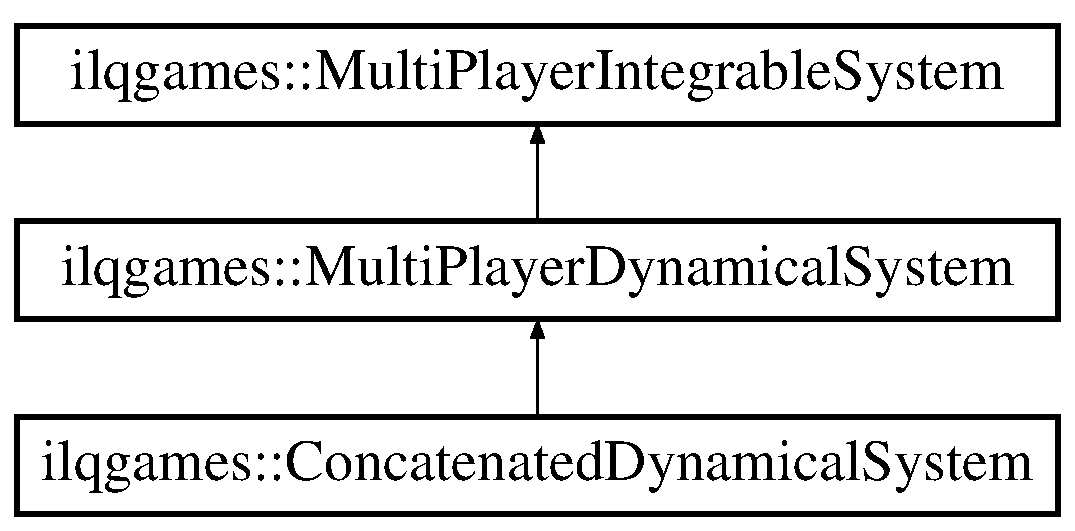
\includegraphics[height=3.000000cm]{classilqgames_1_1_concatenated_dynamical_system}
\end{center}
\end{figure}
\subsection*{Public Member Functions}
\begin{DoxyCompactItemize}
\item 
{\bfseries Concatenated\+Dynamical\+System} (const Subsystem\+List \&subsystems, Time time\+\_\+step)\hypertarget{classilqgames_1_1_concatenated_dynamical_system_afbac1f5e7a0ceaa9b59a0354e959266f}{}\label{classilqgames_1_1_concatenated_dynamical_system_afbac1f5e7a0ceaa9b59a0354e959266f}

\item 
Vector\+Xf {\bfseries Evaluate} (Time t, const Vector\+Xf \&x, const std\+::vector$<$ Vector\+Xf $>$ \&us) const \hypertarget{classilqgames_1_1_concatenated_dynamical_system_aba82e3499a437d6c27c8575f0e749298}{}\label{classilqgames_1_1_concatenated_dynamical_system_aba82e3499a437d6c27c8575f0e749298}

\item 
\hyperlink{structilqgames_1_1_linear_dynamics_approximation}{Linear\+Dynamics\+Approximation} {\bfseries Linearize} (Time t, const Vector\+Xf \&x, const std\+::vector$<$ Vector\+Xf $>$ \&us) const \hypertarget{classilqgames_1_1_concatenated_dynamical_system_a9939297ff3859abc1cf0ad6207783167}{}\label{classilqgames_1_1_concatenated_dynamical_system_a9939297ff3859abc1cf0ad6207783167}

\item 
float {\bfseries Distance\+Between} (const Vector\+Xf \&x0, const Vector\+Xf \&x1) const \hypertarget{classilqgames_1_1_concatenated_dynamical_system_a5d241472286d6f3e49b38c02e47d25f1}{}\label{classilqgames_1_1_concatenated_dynamical_system_a5d241472286d6f3e49b38c02e47d25f1}

\item 
Vector\+Xf {\bfseries Stitch} (const Vector\+Xf \&x\+\_\+ego, const Vector\+Xf \&x\+\_\+others) const \hypertarget{classilqgames_1_1_concatenated_dynamical_system_a81183125fda71b1d57a1630d27f21d98}{}\label{classilqgames_1_1_concatenated_dynamical_system_a81183125fda71b1d57a1630d27f21d98}

\item 
const Subsystem\+List \& {\bfseries Subsystems} () const \hypertarget{classilqgames_1_1_concatenated_dynamical_system_a8556844c77ee4445d47f11a327d19192}{}\label{classilqgames_1_1_concatenated_dynamical_system_a8556844c77ee4445d47f11a327d19192}

\item 
Player\+Index {\bfseries Num\+Players} () const \hypertarget{classilqgames_1_1_concatenated_dynamical_system_a81821c7e9776a45b319f7153bcd93248}{}\label{classilqgames_1_1_concatenated_dynamical_system_a81821c7e9776a45b319f7153bcd93248}

\item 
Dimension {\bfseries Subsystem\+X\+Dim} (Player\+Index player\+\_\+idx) const \hypertarget{classilqgames_1_1_concatenated_dynamical_system_a8a41a816bf3320cd6d78548beac02d80}{}\label{classilqgames_1_1_concatenated_dynamical_system_a8a41a816bf3320cd6d78548beac02d80}

\item 
Dimension {\bfseries U\+Dim} (Player\+Index player\+\_\+idx) const \hypertarget{classilqgames_1_1_concatenated_dynamical_system_a99e27c1644875b924741e037bcb54460}{}\label{classilqgames_1_1_concatenated_dynamical_system_a99e27c1644875b924741e037bcb54460}

\end{DoxyCompactItemize}
\subsection*{Additional Inherited Members}


\subsection{Detailed Description}


Definition at line 55 of file concatenated\+\_\+dynamical\+\_\+system.\+h.



The documentation for this class was generated from the following files\+:\begin{DoxyCompactItemize}
\item 
/home/travis/build/\+H\+J\+Reachability/ilqgames/include/ilqgames/dynamics/concatenated\+\_\+dynamical\+\_\+system.\+h\item 
/home/travis/build/\+H\+J\+Reachability/ilqgames/src/concatenated\+\_\+dynamical\+\_\+system.\+cpp\end{DoxyCompactItemize}

\hypertarget{classilqgames_1_1_concatenated_flat_system}{}\section{ilqgames\+:\+:Concatenated\+Flat\+System Class Reference}
\label{classilqgames_1_1_concatenated_flat_system}\index{ilqgames\+::\+Concatenated\+Flat\+System@{ilqgames\+::\+Concatenated\+Flat\+System}}
Inheritance diagram for ilqgames\+:\+:Concatenated\+Flat\+System\+:\begin{figure}[H]
\begin{center}
\leavevmode
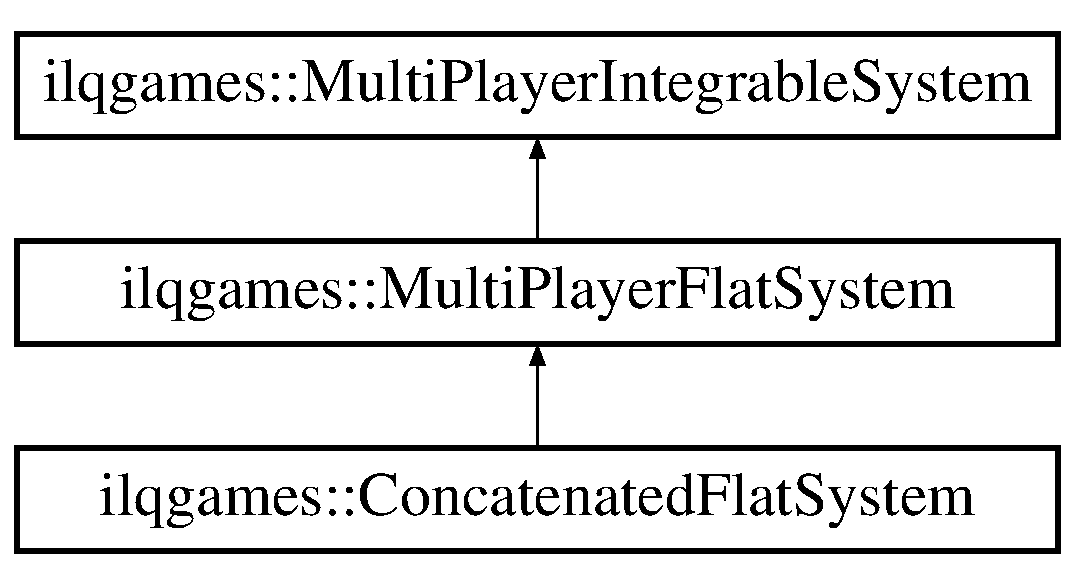
\includegraphics[height=3.000000cm]{classilqgames_1_1_concatenated_flat_system}
\end{center}
\end{figure}
\subsection*{Public Member Functions}
\begin{DoxyCompactItemize}
\item 
{\bfseries Concatenated\+Flat\+System} (const Flat\+Subsystem\+List \&subsystems)\hypertarget{classilqgames_1_1_concatenated_flat_system_ab0efbf94aae2b6a62c1ff2e42edbf590}{}\label{classilqgames_1_1_concatenated_flat_system_ab0efbf94aae2b6a62c1ff2e42edbf590}

\item 
Vector\+Xf {\bfseries Evaluate} (const Vector\+Xf \&x, const std\+::vector$<$ Vector\+Xf $>$ \&us) const \hypertarget{classilqgames_1_1_concatenated_flat_system_aa66c46c672ba365b02abb639feff4320}{}\label{classilqgames_1_1_concatenated_flat_system_aa66c46c672ba365b02abb639feff4320}

\item 
void {\bfseries Compute\+Linearized\+System} () const \hypertarget{classilqgames_1_1_concatenated_flat_system_a61ec103cf78e138c7c91b98af0d922ee}{}\label{classilqgames_1_1_concatenated_flat_system_a61ec103cf78e138c7c91b98af0d922ee}

\item 
Matrix\+Xf {\bfseries Inverse\+Decoupling\+Matrix} (const Vector\+Xf \&x) const \hypertarget{classilqgames_1_1_concatenated_flat_system_a1ddfbabea2c6a2f58d013ee4d919cb31}{}\label{classilqgames_1_1_concatenated_flat_system_a1ddfbabea2c6a2f58d013ee4d919cb31}

\item 
Vector\+Xf {\bfseries Affine\+Term} (const Vector\+Xf \&x) const \hypertarget{classilqgames_1_1_concatenated_flat_system_a4cd24cf9e78380c9752bfd398dd524c3}{}\label{classilqgames_1_1_concatenated_flat_system_a4cd24cf9e78380c9752bfd398dd524c3}

\item 
Vector\+Xf {\bfseries Linearizing\+Control} (const Vector\+Xf \&x, const Vector\+Xf \&v, Player\+Index player) const \hypertarget{classilqgames_1_1_concatenated_flat_system_a396cef9dc50fb39896f917b33681310a}{}\label{classilqgames_1_1_concatenated_flat_system_a396cef9dc50fb39896f917b33681310a}

\item 
std\+::vector$<$ Vector\+Xf $>$ {\bfseries Linearizing\+Controls} (const Vector\+Xf \&x, const std\+::vector$<$ Vector\+Xf $>$ \&vs) const \hypertarget{classilqgames_1_1_concatenated_flat_system_a1bd90fe0f1198f7934d478f0c17db1d4}{}\label{classilqgames_1_1_concatenated_flat_system_a1bd90fe0f1198f7934d478f0c17db1d4}

\item 
Vector\+Xf {\bfseries To\+Linear\+System\+State} (const Vector\+Xf \&x) const \hypertarget{classilqgames_1_1_concatenated_flat_system_a032bc555367ecd4122ec5968962cfff5}{}\label{classilqgames_1_1_concatenated_flat_system_a032bc555367ecd4122ec5968962cfff5}

\item 
Vector\+Xf {\bfseries To\+Linear\+System\+State} (const Vector\+Xf \&x, Player\+Index subsystem\+\_\+idx) const \hypertarget{classilqgames_1_1_concatenated_flat_system_ada597e4306beabae2d83f68ded70823f}{}\label{classilqgames_1_1_concatenated_flat_system_ada597e4306beabae2d83f68ded70823f}

\item 
Vector\+Xf {\bfseries From\+Linear\+System\+State} (const Vector\+Xf \&xi) const \hypertarget{classilqgames_1_1_concatenated_flat_system_aab7969ca5f64a1b670e075aabc32e621}{}\label{classilqgames_1_1_concatenated_flat_system_aab7969ca5f64a1b670e075aabc32e621}

\item 
Vector\+Xf {\bfseries From\+Linear\+System\+State} (const Vector\+Xf \&xi, Player\+Index subsystem\+\_\+idx) const \hypertarget{classilqgames_1_1_concatenated_flat_system_a330952bb97f5cef2130f2166ad6daab6}{}\label{classilqgames_1_1_concatenated_flat_system_a330952bb97f5cef2130f2166ad6daab6}

\item 
bool {\bfseries Is\+Linear\+System\+State\+Singular} (const Vector\+Xf \&xi) const \hypertarget{classilqgames_1_1_concatenated_flat_system_abc379d1ab97515b32e6b5e2e6ec5cf69}{}\label{classilqgames_1_1_concatenated_flat_system_abc379d1ab97515b32e6b5e2e6ec5cf69}

\item 
Vector\+Xf {\bfseries Subsystem\+States} (const Vector\+Xf \&x, Player\+Index subsystem\+\_\+idx) const \hypertarget{classilqgames_1_1_concatenated_flat_system_af1ee81770be11dd9f301c0b2b7f608c0}{}\label{classilqgames_1_1_concatenated_flat_system_af1ee81770be11dd9f301c0b2b7f608c0}

\item 
void {\bfseries Change\+Cost\+Coordinates} (const Vector\+Xf \&xi, std\+::vector$<$ \hyperlink{structilqgames_1_1_quadratic_cost_approximation}{Quadratic\+Cost\+Approximation} $>$ $\ast$q) const \hypertarget{classilqgames_1_1_concatenated_flat_system_a79b8c2249adef578e42cfd92224a45ee}{}\label{classilqgames_1_1_concatenated_flat_system_a79b8c2249adef578e42cfd92224a45ee}

\item 
void {\bfseries Change\+Control\+Cost\+Coordinates} (const Vector\+Xf \&xi, std\+::vector$<$ \hyperlink{structilqgames_1_1_quadratic_cost_approximation}{Quadratic\+Cost\+Approximation} $>$ $\ast$q) const \hypertarget{classilqgames_1_1_concatenated_flat_system_a41de9dc81c1e121c0967f6c6f9a1e966}{}\label{classilqgames_1_1_concatenated_flat_system_a41de9dc81c1e121c0967f6c6f9a1e966}

\item 
float {\bfseries Distance\+Between} (const Vector\+Xf \&x0, const Vector\+Xf \&x1) const \hypertarget{classilqgames_1_1_concatenated_flat_system_aa8d39832e2b73f2666415639e02ccc4e}{}\label{classilqgames_1_1_concatenated_flat_system_aa8d39832e2b73f2666415639e02ccc4e}

\item 
const Flat\+Subsystem\+List \& {\bfseries Subsystems} () const \hypertarget{classilqgames_1_1_concatenated_flat_system_a85bf62fb46eb94efe02131b6f73f0157}{}\label{classilqgames_1_1_concatenated_flat_system_a85bf62fb46eb94efe02131b6f73f0157}

\item 
Player\+Index {\bfseries Num\+Players} () const \hypertarget{classilqgames_1_1_concatenated_flat_system_a502e29574127d8dc373beeab9306edde}{}\label{classilqgames_1_1_concatenated_flat_system_a502e29574127d8dc373beeab9306edde}

\item 
Dimension {\bfseries Subsystem\+X\+Dim} (Player\+Index player\+\_\+idx) const \hypertarget{classilqgames_1_1_concatenated_flat_system_ab721151b47937d8a8f4523b2a1ef12f1}{}\label{classilqgames_1_1_concatenated_flat_system_ab721151b47937d8a8f4523b2a1ef12f1}

\item 
Dimension {\bfseries Subsystem\+Start\+Dim} (Player\+Index player\+\_\+idx) const \hypertarget{classilqgames_1_1_concatenated_flat_system_af2aa76a51e22b4fa744b1f8e425216ff}{}\label{classilqgames_1_1_concatenated_flat_system_af2aa76a51e22b4fa744b1f8e425216ff}

\item 
Dimension {\bfseries U\+Dim} (Player\+Index player\+\_\+idx) const \hypertarget{classilqgames_1_1_concatenated_flat_system_a2cb3c62d20eeac814f1b72e4d8355b80}{}\label{classilqgames_1_1_concatenated_flat_system_a2cb3c62d20eeac814f1b72e4d8355b80}

\item 
std\+::vector$<$ Dimension $>$ {\bfseries Position\+Dimensions} () const \hypertarget{classilqgames_1_1_concatenated_flat_system_a31dc8d20b0735223ce285262c17286f6}{}\label{classilqgames_1_1_concatenated_flat_system_a31dc8d20b0735223ce285262c17286f6}

\end{DoxyCompactItemize}
\subsection*{Additional Inherited Members}


\subsection{Detailed Description}


Definition at line 56 of file concatenated\+\_\+flat\+\_\+system.\+h.



The documentation for this class was generated from the following files\+:\begin{DoxyCompactItemize}
\item 
/home/travis/build/\+H\+J\+Reachability/ilqgames/include/ilqgames/dynamics/concatenated\+\_\+flat\+\_\+system.\+h\item 
/home/travis/build/\+H\+J\+Reachability/ilqgames/src/concatenated\+\_\+flat\+\_\+system.\+cpp\end{DoxyCompactItemize}

\hypertarget{classilqgames_1_1_constraint}{}\section{ilqgames\+:\+:Constraint Class Reference}
\label{classilqgames_1_1_constraint}\index{ilqgames\+::\+Constraint@{ilqgames\+::\+Constraint}}
Inheritance diagram for ilqgames\+:\+:Constraint\+:\begin{figure}[H]
\begin{center}
\leavevmode
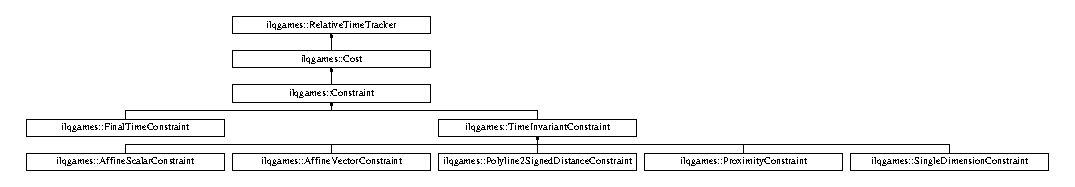
\includegraphics[height=2.755228cm]{classilqgames_1_1_constraint}
\end{center}
\end{figure}
\subsection*{Public Member Functions}
\begin{DoxyCompactItemize}
\item 
void {\bfseries Reset\+Barrier\+Weight} ()\hypertarget{classilqgames_1_1_constraint_af282fb2fae6fa61301c1f900899a388c}{}\label{classilqgames_1_1_constraint_af282fb2fae6fa61301c1f900899a388c}

\item 
void {\bfseries Scale\+Barrier\+Weight} (float scale)\hypertarget{classilqgames_1_1_constraint_a6474f6bbb0b2170254491062312e70f1}{}\label{classilqgames_1_1_constraint_a6474f6bbb0b2170254491062312e70f1}

\item 
virtual bool {\bfseries Is\+Satisfied\+Level} (Time t, const Vector\+Xf \&input, float $\ast$level) const =0\hypertarget{classilqgames_1_1_constraint_a1b2c7e1b5b29c9728502cc51a82d0edb}{}\label{classilqgames_1_1_constraint_a1b2c7e1b5b29c9728502cc51a82d0edb}

\item 
bool {\bfseries Is\+Satisfied} (Time t, const Vector\+Xf \&input) const \hypertarget{classilqgames_1_1_constraint_a2a7322945a8a57720c7fa48cf48eadb0}{}\label{classilqgames_1_1_constraint_a2a7322945a8a57720c7fa48cf48eadb0}

\item 
float {\bfseries Evaluate} (Time t, const Vector\+Xf \&input) const \hypertarget{classilqgames_1_1_constraint_aa9d8f8f9cf80d4de4e861c00d8e04df8}{}\label{classilqgames_1_1_constraint_aa9d8f8f9cf80d4de4e861c00d8e04df8}

\item 
virtual void {\bfseries Quadraticize} (Time t, const Vector\+Xf \&input, Matrix\+Xf $\ast$hess, Vector\+Xf $\ast$grad) const =0\hypertarget{classilqgames_1_1_constraint_a94538ad0da7e881d1a3bd4009c43f775}{}\label{classilqgames_1_1_constraint_a94538ad0da7e881d1a3bd4009c43f775}

\item 
const \hyperlink{classilqgames_1_1_cost}{Cost} \& {\bfseries Equivalent\+Cost} () const \hypertarget{classilqgames_1_1_constraint_a01d415fabb97d12b0c8b6f88bfc29f6f}{}\label{classilqgames_1_1_constraint_a01d415fabb97d12b0c8b6f88bfc29f6f}

\end{DoxyCompactItemize}
\subsection*{Protected Member Functions}
\begin{DoxyCompactItemize}
\item 
{\bfseries Constraint} (const std\+::string \&name=\char`\"{}\char`\"{})\hypertarget{classilqgames_1_1_constraint_a845ad9283a9921452afa22c34404302c}{}\label{classilqgames_1_1_constraint_a845ad9283a9921452afa22c34404302c}

\end{DoxyCompactItemize}
\subsection*{Protected Attributes}
\begin{DoxyCompactItemize}
\item 
std\+::unique\+\_\+ptr$<$ \hyperlink{classilqgames_1_1_cost}{Cost} $>$ {\bfseries equivalent\+\_\+cost\+\_\+}\hypertarget{classilqgames_1_1_constraint_aa33d6b05a13fe556b844656f07753e37}{}\label{classilqgames_1_1_constraint_aa33d6b05a13fe556b844656f07753e37}

\end{DoxyCompactItemize}
\subsection*{Static Protected Attributes}
\begin{DoxyCompactItemize}
\item 
static constexpr float {\bfseries k\+Initial\+Barrier\+Weight} = 1.\+0\hypertarget{classilqgames_1_1_constraint_a1c1566fc2fa74e58b54fae57c07b7af8}{}\label{classilqgames_1_1_constraint_a1c1566fc2fa74e58b54fae57c07b7af8}

\item 
static constexpr float {\bfseries k\+Initial\+Equivalent\+Cost\+Weight} = 0.\+0\hypertarget{classilqgames_1_1_constraint_a64fd12449a7f42d19c68b568140699a3}{}\label{classilqgames_1_1_constraint_a64fd12449a7f42d19c68b568140699a3}

\item 
static constexpr float {\bfseries k\+Cost\+Buffer} = 0.\+1\hypertarget{classilqgames_1_1_constraint_aaef1da643690381eca61569190863129}{}\label{classilqgames_1_1_constraint_aaef1da643690381eca61569190863129}

\end{DoxyCompactItemize}
\subsection*{Additional Inherited Members}


\subsection{Detailed Description}


Definition at line 61 of file constraint.\+h.



The documentation for this class was generated from the following files\+:\begin{DoxyCompactItemize}
\item 
/home/travis/build/\+H\+J\+Reachability/ilqgames/include/ilqgames/constraint/constraint.\+h\item 
/home/travis/build/\+H\+J\+Reachability/ilqgames/src/constraint.\+cpp\end{DoxyCompactItemize}

\hypertarget{classilqgames_1_1_control_sliders}{}\section{ilqgames\+:\+:Control\+Sliders Class Reference}
\label{classilqgames_1_1_control_sliders}\index{ilqgames\+::\+Control\+Sliders@{ilqgames\+::\+Control\+Sliders}}
\subsection*{Public Member Functions}
\begin{DoxyCompactItemize}
\item 
{\bfseries Control\+Sliders} (const std\+::vector$<$ std\+::vector$<$ std\+::shared\+\_\+ptr$<$ const \hyperlink{classilqgames_1_1_solver_log}{ilqgames\+::\+Solver\+Log} $>$$>$$>$ \&logs\+\_\+for\+\_\+each\+\_\+problem)\hypertarget{classilqgames_1_1_control_sliders_a87f44ac674d284ac368daca4c1fff949}{}\label{classilqgames_1_1_control_sliders_a87f44ac674d284ac368daca4c1fff949}

\item 
void {\bfseries Render} ()\hypertarget{classilqgames_1_1_control_sliders_a06886eb116592138d8f9340430e4d30d}{}\label{classilqgames_1_1_control_sliders_a06886eb116592138d8f9340430e4d30d}

\item 
size\+\_\+t {\bfseries Num\+Problems} () const \hypertarget{classilqgames_1_1_control_sliders_ae3752e7499e913dc3bbb46e19061cf11}{}\label{classilqgames_1_1_control_sliders_ae3752e7499e913dc3bbb46e19061cf11}

\item 
const std\+::vector$<$ std\+::vector$<$ std\+::shared\+\_\+ptr$<$ const \hyperlink{classilqgames_1_1_solver_log}{Solver\+Log} $>$ $>$ $>$ \& {\bfseries Logs\+For\+Each\+Problem} () const \hypertarget{classilqgames_1_1_control_sliders_a255c57dd31398f88b808fd9bf936b2b1}{}\label{classilqgames_1_1_control_sliders_a255c57dd31398f88b808fd9bf936b2b1}

\item 
std\+::vector$<$ std\+::shared\+\_\+ptr$<$ const \hyperlink{classilqgames_1_1_solver_log}{Solver\+Log} $>$ $>$ {\bfseries Log\+For\+Each\+Problem} () const \hypertarget{classilqgames_1_1_control_sliders_ade4d6dab5db6ca493881c769e2ce9944}{}\label{classilqgames_1_1_control_sliders_ade4d6dab5db6ca493881c769e2ce9944}

\item 
Time {\bfseries Interpolation\+Time} (size\+\_\+t problem\+\_\+idx) const \hypertarget{classilqgames_1_1_control_sliders_a7619ee44e6ce84b5df323a6493338a72}{}\label{classilqgames_1_1_control_sliders_a7619ee44e6ce84b5df323a6493338a72}

\item 
int {\bfseries Solver\+Iterate} (size\+\_\+t problem\+\_\+idx) const \hypertarget{classilqgames_1_1_control_sliders_a1963e1ac97100303f6d0ad8483e7340f}{}\label{classilqgames_1_1_control_sliders_a1963e1ac97100303f6d0ad8483e7340f}

\item 
int {\bfseries Log\+Index} (size\+\_\+t problem\+\_\+idx) const \hypertarget{classilqgames_1_1_control_sliders_ae5dd8db5d88f8d8c1d8e2a23b25e1ab5}{}\label{classilqgames_1_1_control_sliders_ae5dd8db5d88f8d8c1d8e2a23b25e1ab5}

\item 
int {\bfseries Max\+Log\+Index} () const \hypertarget{classilqgames_1_1_control_sliders_a370e35a28a451951d9cadcd58172b853}{}\label{classilqgames_1_1_control_sliders_a370e35a28a451951d9cadcd58172b853}

\end{DoxyCompactItemize}


\subsection{Detailed Description}


Definition at line 53 of file control\+\_\+sliders.\+h.



The documentation for this class was generated from the following files\+:\begin{DoxyCompactItemize}
\item 
/home/travis/build/\+H\+J\+Reachability/ilqgames/include/ilqgames/gui/control\+\_\+sliders.\+h\item 
/home/travis/build/\+H\+J\+Reachability/ilqgames/src/control\+\_\+sliders.\+cpp\end{DoxyCompactItemize}

\hypertarget{classilqgames_1_1_cost}{}\section{ilqgames\+:\+:Cost Class Reference}
\label{classilqgames_1_1_cost}\index{ilqgames\+::\+Cost@{ilqgames\+::\+Cost}}
Inheritance diagram for ilqgames\+:\+:Cost\+:\begin{figure}[H]
\begin{center}
\leavevmode
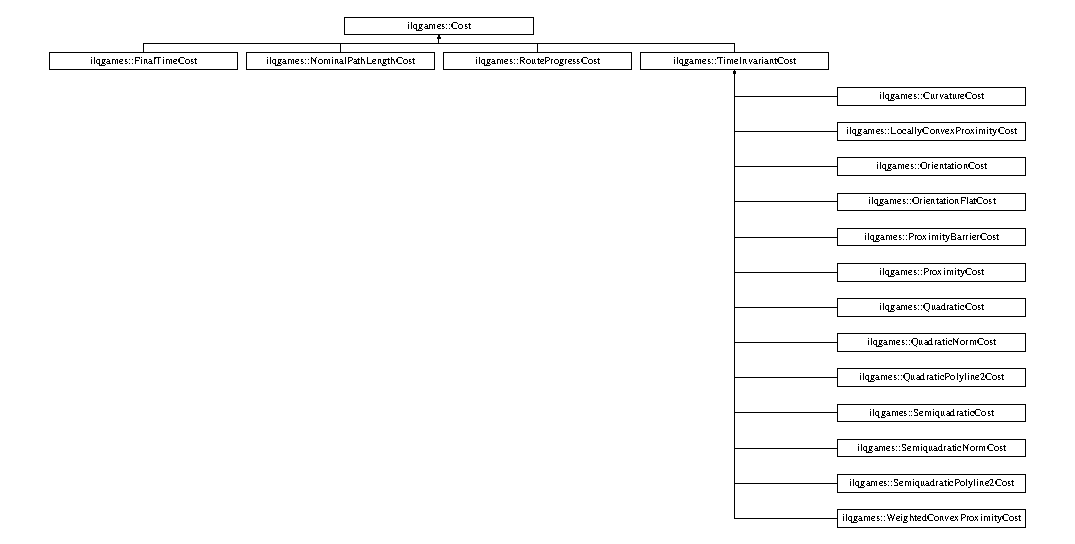
\includegraphics[height=6.857143cm]{classilqgames_1_1_cost}
\end{center}
\end{figure}
\subsection*{Public Member Functions}
\begin{DoxyCompactItemize}
\item 
virtual float {\bfseries Evaluate} (Time t, const Vector\+Xf \&input) const =0\hypertarget{classilqgames_1_1_cost_a90ad7fc2697f0d8c3392dc5a079e40f9}{}\label{classilqgames_1_1_cost_a90ad7fc2697f0d8c3392dc5a079e40f9}

\item 
virtual void {\bfseries Quadraticize} (Time t, const Vector\+Xf \&input, Matrix\+Xf $\ast$hess, Vector\+Xf $\ast$grad=nullptr) const =0\hypertarget{classilqgames_1_1_cost_ade89b117df8b8ec0e491d121f9682aef}{}\label{classilqgames_1_1_cost_ade89b117df8b8ec0e491d121f9682aef}

\item 
const std\+::string \& {\bfseries Name} () const \hypertarget{classilqgames_1_1_cost_a7e21af3d7f23aee0d913ad5e2e0292cb}{}\label{classilqgames_1_1_cost_a7e21af3d7f23aee0d913ad5e2e0292cb}

\end{DoxyCompactItemize}
\subsection*{Protected Member Functions}
\begin{DoxyCompactItemize}
\item 
{\bfseries Cost} (float weight, const std\+::string \&name=\char`\"{}\char`\"{})\hypertarget{classilqgames_1_1_cost_a9b30ac1d7733741609a3c8d6522a925b}{}\label{classilqgames_1_1_cost_a9b30ac1d7733741609a3c8d6522a925b}

\end{DoxyCompactItemize}
\subsection*{Protected Attributes}
\begin{DoxyCompactItemize}
\item 
const float {\bfseries weight\+\_\+}\hypertarget{classilqgames_1_1_cost_a9d23ad75587bd930e9d63bd53532f688}{}\label{classilqgames_1_1_cost_a9d23ad75587bd930e9d63bd53532f688}

\item 
const std\+::string {\bfseries name\+\_\+}\hypertarget{classilqgames_1_1_cost_a36d7d9ee9585912fc98fca10d9c81614}{}\label{classilqgames_1_1_cost_a36d7d9ee9585912fc98fca10d9c81614}

\end{DoxyCompactItemize}


\subsection{Detailed Description}


Definition at line 55 of file cost.\+h.



The documentation for this class was generated from the following file\+:\begin{DoxyCompactItemize}
\item 
/home/travis/build/\+H\+J\+Reachability/ilqgames/include/ilqgames/cost/cost.\+h\end{DoxyCompactItemize}

\hypertarget{classilqgames_1_1_cost_inspector}{}\section{ilqgames\+:\+:Cost\+Inspector Class Reference}
\label{classilqgames_1_1_cost_inspector}\index{ilqgames\+::\+Cost\+Inspector@{ilqgames\+::\+Cost\+Inspector}}
\subsection*{Public Member Functions}
\begin{DoxyCompactItemize}
\item 
{\bfseries Cost\+Inspector} (const std\+::shared\+\_\+ptr$<$ const \hyperlink{classilqgames_1_1_control_sliders}{Control\+Sliders} $>$ \&sliders, const std\+::vector$<$ std\+::vector$<$ \hyperlink{classilqgames_1_1_player_cost}{Player\+Cost} $>$$>$ \&player\+\_\+costs)\hypertarget{classilqgames_1_1_cost_inspector_a40b12f9b1646636615d5e0f00ebd0814}{}\label{classilqgames_1_1_cost_inspector_a40b12f9b1646636615d5e0f00ebd0814}

\item 
void {\bfseries Render} () const \hypertarget{classilqgames_1_1_cost_inspector_af6ccfb7db9e5672ee1798019b6aac177}{}\label{classilqgames_1_1_cost_inspector_af6ccfb7db9e5672ee1798019b6aac177}

\end{DoxyCompactItemize}


\subsection{Detailed Description}


Definition at line 62 of file cost\+\_\+inspector.\+h.



The documentation for this class was generated from the following files\+:\begin{DoxyCompactItemize}
\item 
/home/travis/build/\+H\+J\+Reachability/ilqgames/include/ilqgames/gui/cost\+\_\+inspector.\+h\item 
/home/travis/build/\+H\+J\+Reachability/ilqgames/src/cost\+\_\+inspector.\+cpp\end{DoxyCompactItemize}

\hypertarget{classilqgames_1_1_curvature_cost}{}\section{ilqgames\+:\+:Curvature\+Cost Class Reference}
\label{classilqgames_1_1_curvature_cost}\index{ilqgames\+::\+Curvature\+Cost@{ilqgames\+::\+Curvature\+Cost}}
Inheritance diagram for ilqgames\+:\+:Curvature\+Cost\+:\begin{figure}[H]
\begin{center}
\leavevmode
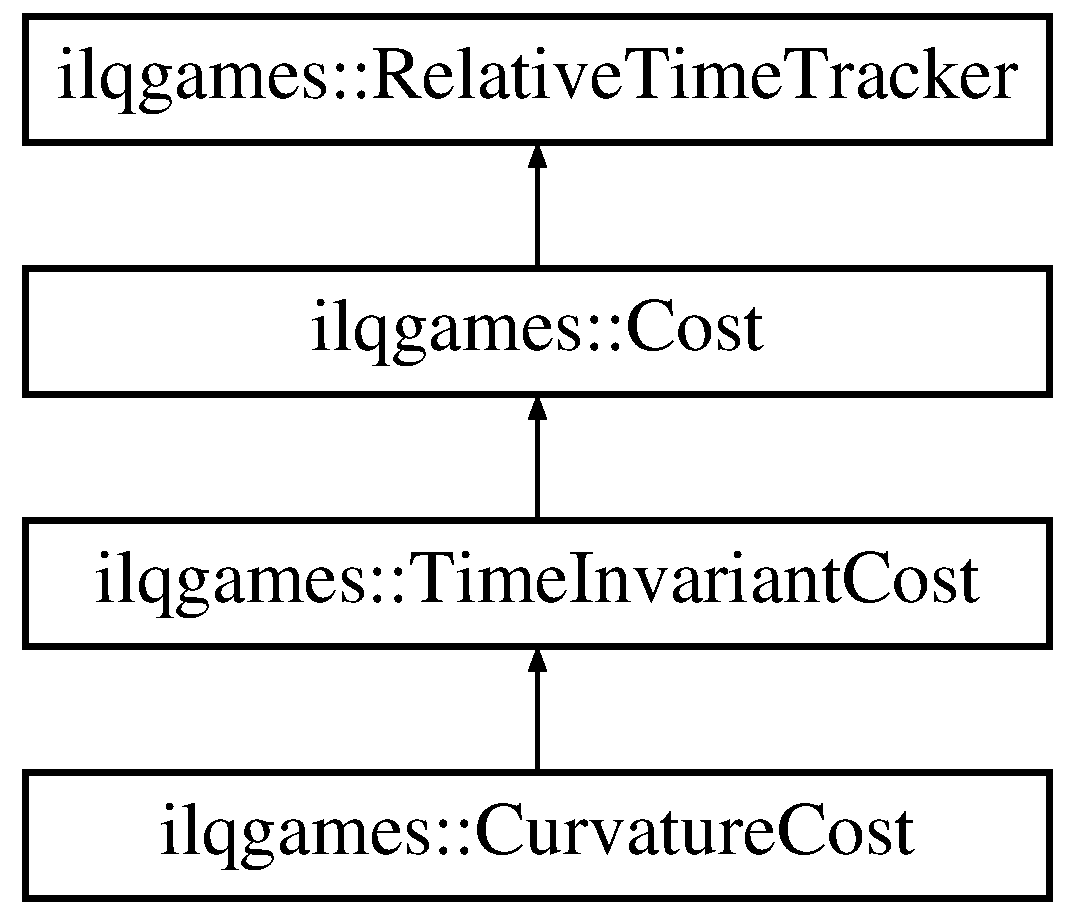
\includegraphics[height=3.000000cm]{classilqgames_1_1_curvature_cost}
\end{center}
\end{figure}
\subsection*{Public Member Functions}
\begin{DoxyCompactItemize}
\item 
{\bfseries Curvature\+Cost} (float weight, Dimension omega\+\_\+idx, Dimension v\+\_\+idx, const std\+::string \&name=\char`\"{}\char`\"{})\hypertarget{classilqgames_1_1_curvature_cost_af3cef5c86cf6412de31496c1f7cc074a}{}\label{classilqgames_1_1_curvature_cost_af3cef5c86cf6412de31496c1f7cc074a}

\item 
float {\bfseries Evaluate} (const Vector\+Xf \&input) const \hypertarget{classilqgames_1_1_curvature_cost_a112ce04ef70a60c83d80a3de01108248}{}\label{classilqgames_1_1_curvature_cost_a112ce04ef70a60c83d80a3de01108248}

\item 
void {\bfseries Quadraticize} (const Vector\+Xf \&input, Matrix\+Xf $\ast$hess, Vector\+Xf $\ast$grad) const \hypertarget{classilqgames_1_1_curvature_cost_af35cbf73cd158328d60396d7411e8516}{}\label{classilqgames_1_1_curvature_cost_af35cbf73cd158328d60396d7411e8516}

\end{DoxyCompactItemize}
\subsection*{Additional Inherited Members}


\subsection{Detailed Description}


Definition at line 53 of file curvature\+\_\+cost.\+h.



The documentation for this class was generated from the following files\+:\begin{DoxyCompactItemize}
\item 
/home/travis/build/\+H\+J\+Reachability/ilqgames/include/ilqgames/cost/curvature\+\_\+cost.\+h\item 
/home/travis/build/\+H\+J\+Reachability/ilqgames/src/curvature\+\_\+cost.\+cpp\end{DoxyCompactItemize}

\hypertarget{classilqgames_1_1_dubins_origin_example}{}\section{ilqgames\+:\+:Dubins\+Origin\+Example Class Reference}
\label{classilqgames_1_1_dubins_origin_example}\index{ilqgames\+::\+Dubins\+Origin\+Example@{ilqgames\+::\+Dubins\+Origin\+Example}}
Inheritance diagram for ilqgames\+:\+:Dubins\+Origin\+Example\+:\begin{figure}[H]
\begin{center}
\leavevmode
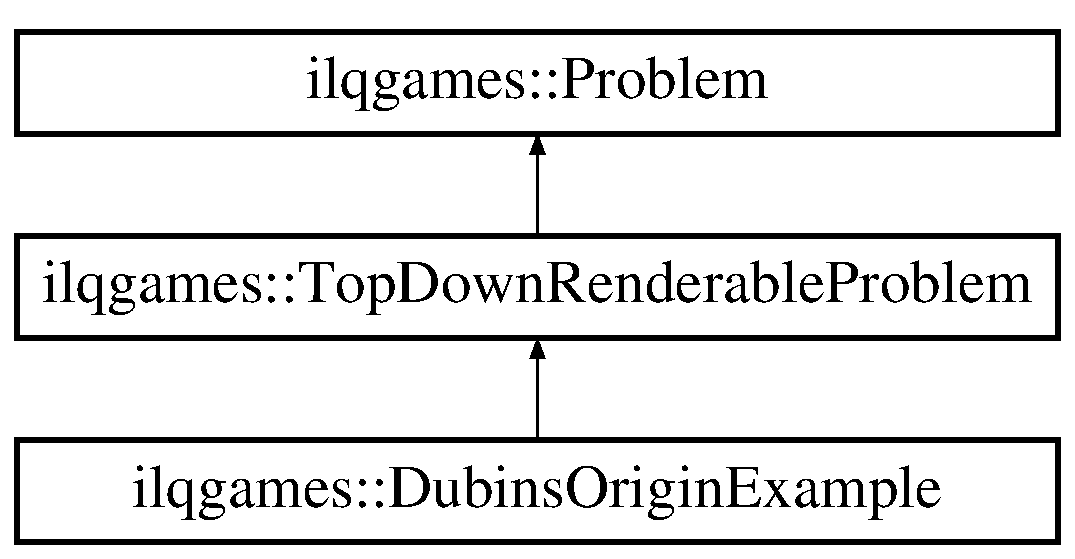
\includegraphics[height=3.000000cm]{classilqgames_1_1_dubins_origin_example}
\end{center}
\end{figure}
\subsection*{Public Member Functions}
\begin{DoxyCompactItemize}
\item 
void {\bfseries Construct\+Dynamics} ()\hypertarget{classilqgames_1_1_dubins_origin_example_a7e7c6f070e3d3d8c2146c7dd2940fa8b}{}\label{classilqgames_1_1_dubins_origin_example_a7e7c6f070e3d3d8c2146c7dd2940fa8b}

\item 
void {\bfseries Construct\+Initial\+State} ()\hypertarget{classilqgames_1_1_dubins_origin_example_abddd656d0a183f6ee064dd4a2e1274a9}{}\label{classilqgames_1_1_dubins_origin_example_abddd656d0a183f6ee064dd4a2e1274a9}

\item 
void {\bfseries Construct\+Player\+Costs} ()\hypertarget{classilqgames_1_1_dubins_origin_example_a634c9d563ae35f524ebdbac9b137a7e0}{}\label{classilqgames_1_1_dubins_origin_example_a634c9d563ae35f524ebdbac9b137a7e0}

\item 
std\+::vector$<$ float $>$ {\bfseries Xs} (const Vector\+Xf \&x) const \hypertarget{classilqgames_1_1_dubins_origin_example_a29910b6c91478b66b64765ce418f5846}{}\label{classilqgames_1_1_dubins_origin_example_a29910b6c91478b66b64765ce418f5846}

\item 
std\+::vector$<$ float $>$ {\bfseries Ys} (const Vector\+Xf \&x) const \hypertarget{classilqgames_1_1_dubins_origin_example_a993f76e0d7549d37973a258c2b78a962}{}\label{classilqgames_1_1_dubins_origin_example_a993f76e0d7549d37973a258c2b78a962}

\item 
std\+::vector$<$ float $>$ {\bfseries Thetas} (const Vector\+Xf \&x) const \hypertarget{classilqgames_1_1_dubins_origin_example_a650be123b88df2bc4fa9c137810b1d6d}{}\label{classilqgames_1_1_dubins_origin_example_a650be123b88df2bc4fa9c137810b1d6d}

\end{DoxyCompactItemize}
\subsection*{Additional Inherited Members}


\subsection{Detailed Description}


Definition at line 55 of file dubins\+\_\+origin\+\_\+example.\+h.



The documentation for this class was generated from the following files\+:\begin{DoxyCompactItemize}
\item 
/home/travis/build/\+H\+J\+Reachability/ilqgames/include/ilqgames/examples/dubins\+\_\+origin\+\_\+example.\+h\item 
/home/travis/build/\+H\+J\+Reachability/ilqgames/src/dubins\+\_\+origin\+\_\+example.\+cpp\end{DoxyCompactItemize}

\hypertarget{structilqgames_1_1_empty}{}\section{ilqgames\+:\+:Empty Struct Reference}
\label{structilqgames_1_1_empty}\index{ilqgames\+::\+Empty@{ilqgames\+::\+Empty}}


\subsection{Detailed Description}


Definition at line 109 of file types.\+h.



The documentation for this struct was generated from the following file\+:\begin{DoxyCompactItemize}
\item 
/home/travis/build/\+H\+J\+Reachability/ilqgames/include/ilqgames/utils/types.\+h\end{DoxyCompactItemize}

\hypertarget{classilqgames_1_1_extreme_value_cost}{}\section{ilqgames\+:\+:Extreme\+Value\+Cost Class Reference}
\label{classilqgames_1_1_extreme_value_cost}\index{ilqgames\+::\+Extreme\+Value\+Cost@{ilqgames\+::\+Extreme\+Value\+Cost}}
Inheritance diagram for ilqgames\+:\+:Extreme\+Value\+Cost\+:\begin{figure}[H]
\begin{center}
\leavevmode
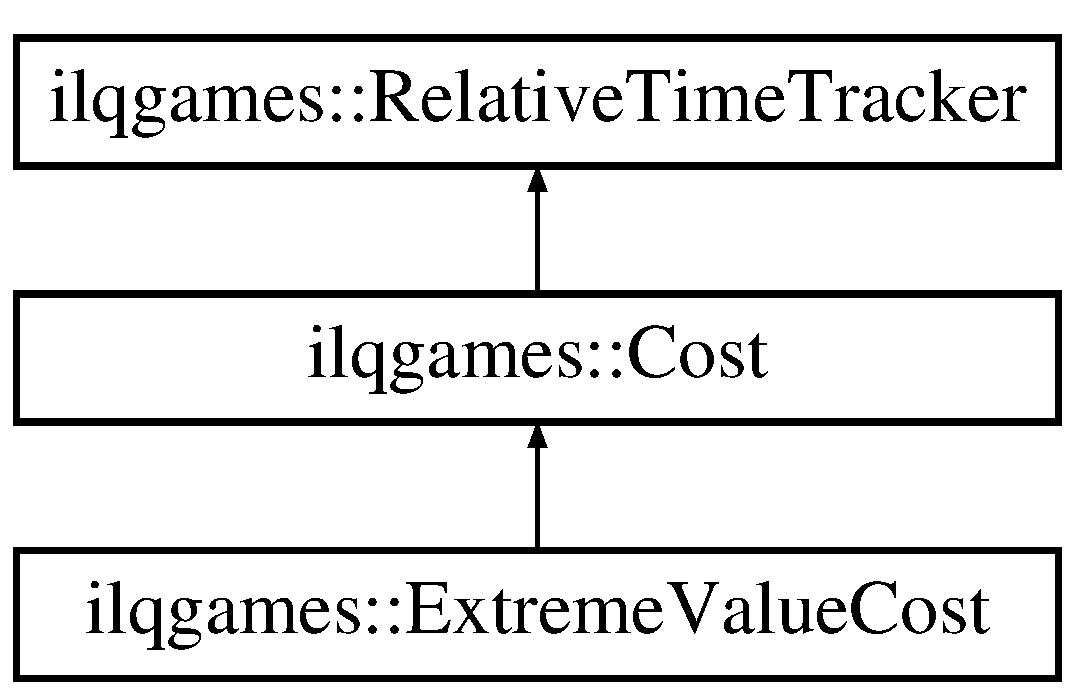
\includegraphics[height=2.000000cm]{classilqgames_1_1_extreme_value_cost}
\end{center}
\end{figure}
\subsection*{Public Member Functions}
\begin{DoxyCompactItemize}
\item 
{\bfseries Extreme\+Value\+Cost} (const std\+::vector$<$ std\+::shared\+\_\+ptr$<$ const \hyperlink{classilqgames_1_1_cost}{Cost} $>$$>$ \&costs, bool is\+\_\+min, const std\+::string \&name=\char`\"{}\char`\"{})\hypertarget{classilqgames_1_1_extreme_value_cost_abfc02bd3700be88b9ac3370d17e1aa78}{}\label{classilqgames_1_1_extreme_value_cost_abfc02bd3700be88b9ac3370d17e1aa78}

\item 
float {\bfseries Evaluate} (Time t, const Vector\+Xf \&input) const \hypertarget{classilqgames_1_1_extreme_value_cost_a90b48a84e25ad4f4c165b6badfb987ba}{}\label{classilqgames_1_1_extreme_value_cost_a90b48a84e25ad4f4c165b6badfb987ba}

\item 
void {\bfseries Quadraticize} (Time t, const Vector\+Xf \&input, Matrix\+Xf $\ast$hess, Vector\+Xf $\ast$grad) const \hypertarget{classilqgames_1_1_extreme_value_cost_ae248e63aededf45ef64481c8174abf53}{}\label{classilqgames_1_1_extreme_value_cost_ae248e63aededf45ef64481c8174abf53}

\item 
const \hyperlink{classilqgames_1_1_cost}{Cost} $\ast$ {\bfseries Extreme\+Cost} (Time t, const Vector\+Xf \&input, float $\ast$evaluated=nullptr) const \hypertarget{classilqgames_1_1_extreme_value_cost_a20c6e9104fb7a84d86828f3204e8d248}{}\label{classilqgames_1_1_extreme_value_cost_a20c6e9104fb7a84d86828f3204e8d248}

\end{DoxyCompactItemize}
\subsection*{Additional Inherited Members}


\subsection{Detailed Description}


Definition at line 54 of file extreme\+\_\+value\+\_\+cost.\+h.



The documentation for this class was generated from the following files\+:\begin{DoxyCompactItemize}
\item 
/home/travis/build/\+H\+J\+Reachability/ilqgames/include/ilqgames/cost/extreme\+\_\+value\+\_\+cost.\+h\item 
/home/travis/build/\+H\+J\+Reachability/ilqgames/src/extreme\+\_\+value\+\_\+cost.\+cpp\end{DoxyCompactItemize}

\hypertarget{classilqgames_1_1_final_time_cost}{}\section{ilqgames\+:\+:Final\+Time\+Cost Class Reference}
\label{classilqgames_1_1_final_time_cost}\index{ilqgames\+::\+Final\+Time\+Cost@{ilqgames\+::\+Final\+Time\+Cost}}
Inheritance diagram for ilqgames\+:\+:Final\+Time\+Cost\+:\begin{figure}[H]
\begin{center}
\leavevmode
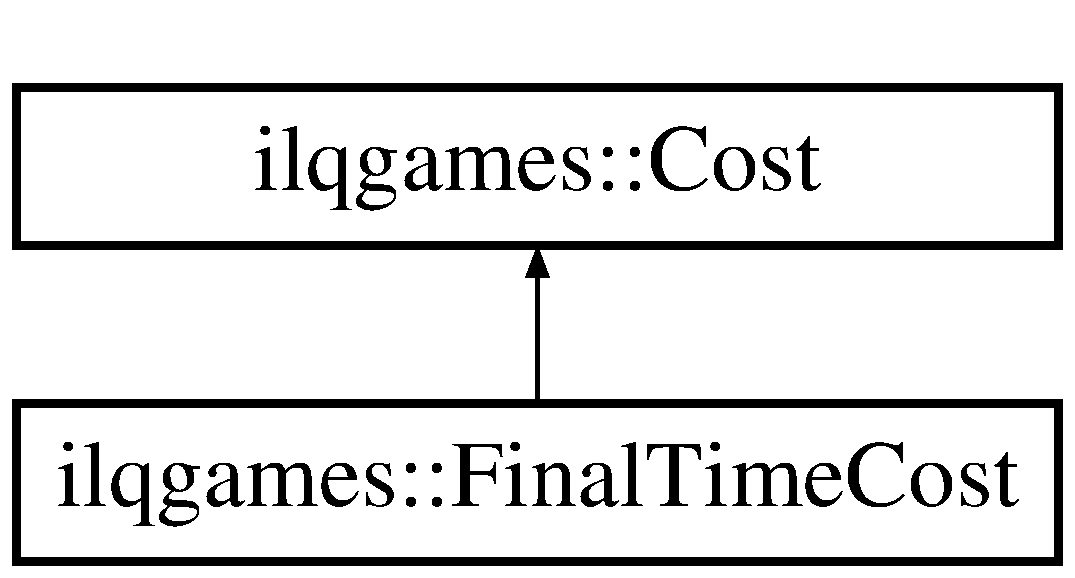
\includegraphics[height=3.000000cm]{classilqgames_1_1_final_time_cost}
\end{center}
\end{figure}
\subsection*{Public Member Functions}
\begin{DoxyCompactItemize}
\item 
{\bfseries Final\+Time\+Cost} (const std\+::shared\+\_\+ptr$<$ const \hyperlink{classilqgames_1_1_cost}{Cost} $>$ \&cost, Time threshold\+\_\+time, const std\+::string \&name=\char`\"{}\char`\"{})\hypertarget{classilqgames_1_1_final_time_cost_a6990af0593d112126a7e327769bfff26}{}\label{classilqgames_1_1_final_time_cost_a6990af0593d112126a7e327769bfff26}

\item 
float {\bfseries Evaluate} (Time t, const Vector\+Xf \&input) const \hypertarget{classilqgames_1_1_final_time_cost_a69d2a9c213b4f25fbd653c6f62790523}{}\label{classilqgames_1_1_final_time_cost_a69d2a9c213b4f25fbd653c6f62790523}

\item 
void {\bfseries Quadraticize} (Time t, const Vector\+Xf \&input, Matrix\+Xf $\ast$hess, Vector\+Xf $\ast$grad) const \hypertarget{classilqgames_1_1_final_time_cost_ab1a60891be81b98096f1009b75d2e230}{}\label{classilqgames_1_1_final_time_cost_ab1a60891be81b98096f1009b75d2e230}

\end{DoxyCompactItemize}
\subsection*{Additional Inherited Members}


\subsection{Detailed Description}


Definition at line 55 of file final\+\_\+time\+\_\+cost.\+h.



The documentation for this class was generated from the following file\+:\begin{DoxyCompactItemize}
\item 
/home/travis/build/\+H\+J\+Reachability/ilqgames/include/ilqgames/cost/final\+\_\+time\+\_\+cost.\+h\end{DoxyCompactItemize}

\hypertarget{classilqgames_1_1_flat_roundabout_merging_example}{}\section{ilqgames\+:\+:Flat\+Roundabout\+Merging\+Example Class Reference}
\label{classilqgames_1_1_flat_roundabout_merging_example}\index{ilqgames\+::\+Flat\+Roundabout\+Merging\+Example@{ilqgames\+::\+Flat\+Roundabout\+Merging\+Example}}
Inheritance diagram for ilqgames\+:\+:Flat\+Roundabout\+Merging\+Example\+:\begin{figure}[H]
\begin{center}
\leavevmode
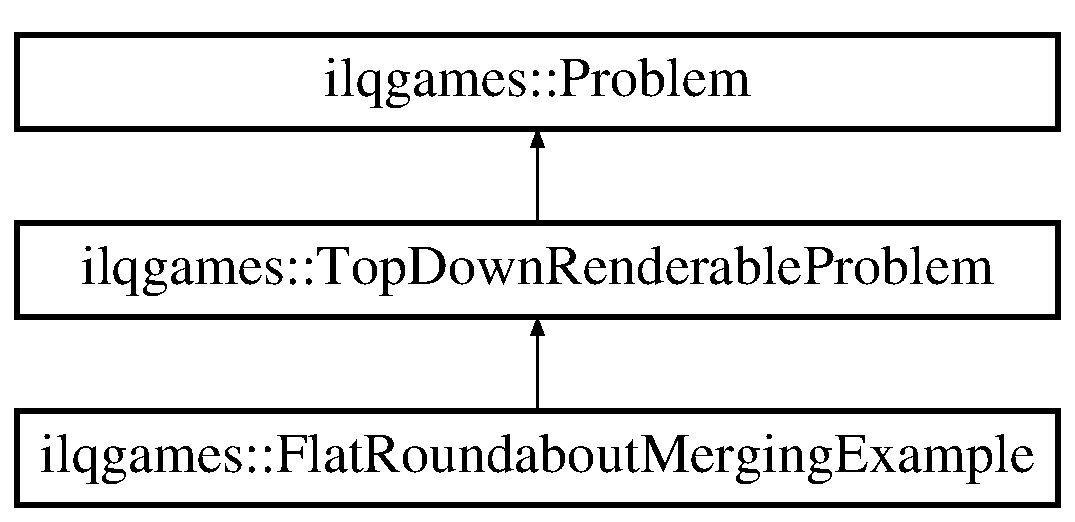
\includegraphics[height=3.000000cm]{classilqgames_1_1_flat_roundabout_merging_example}
\end{center}
\end{figure}
\subsection*{Public Member Functions}
\begin{DoxyCompactItemize}
\item 
void {\bfseries Construct\+Dynamics} ()\hypertarget{classilqgames_1_1_flat_roundabout_merging_example_a5f405d29f89975ba91cdea184e9253ee}{}\label{classilqgames_1_1_flat_roundabout_merging_example_a5f405d29f89975ba91cdea184e9253ee}

\item 
void {\bfseries Construct\+Initial\+State} ()\hypertarget{classilqgames_1_1_flat_roundabout_merging_example_adb289fa37b235aaf17229088e36bf0ea}{}\label{classilqgames_1_1_flat_roundabout_merging_example_adb289fa37b235aaf17229088e36bf0ea}

\item 
void {\bfseries Construct\+Initial\+Operating\+Point} ()\hypertarget{classilqgames_1_1_flat_roundabout_merging_example_a0d45ae5004e887af6480368134281275}{}\label{classilqgames_1_1_flat_roundabout_merging_example_a0d45ae5004e887af6480368134281275}

\item 
void {\bfseries Construct\+Player\+Costs} ()\hypertarget{classilqgames_1_1_flat_roundabout_merging_example_a4f82243cdd8b8d6dfa961cd19162c65e}{}\label{classilqgames_1_1_flat_roundabout_merging_example_a4f82243cdd8b8d6dfa961cd19162c65e}

\item 
std\+::vector$<$ float $>$ {\bfseries Xs} (const Vector\+Xf \&xi) const \hypertarget{classilqgames_1_1_flat_roundabout_merging_example_a19509a51bc48488fad8eb10c979004e7}{}\label{classilqgames_1_1_flat_roundabout_merging_example_a19509a51bc48488fad8eb10c979004e7}

\item 
std\+::vector$<$ float $>$ {\bfseries Ys} (const Vector\+Xf \&xi) const \hypertarget{classilqgames_1_1_flat_roundabout_merging_example_a0f9ec2bd40585eed90f7e6b73d31c1a1}{}\label{classilqgames_1_1_flat_roundabout_merging_example_a0f9ec2bd40585eed90f7e6b73d31c1a1}

\item 
std\+::vector$<$ float $>$ {\bfseries Thetas} (const Vector\+Xf \&xi) const \hypertarget{classilqgames_1_1_flat_roundabout_merging_example_a389cbee0a71f7149c7550a5ea39201a2}{}\label{classilqgames_1_1_flat_roundabout_merging_example_a389cbee0a71f7149c7550a5ea39201a2}

\item 
std\+::shared\+\_\+ptr$<$ const \hyperlink{classilqgames_1_1_concatenated_flat_system}{Concatenated\+Flat\+System} $>$ {\bfseries Dynamics} () const \hypertarget{classilqgames_1_1_flat_roundabout_merging_example_abb8e4df38141924f3072e9151b6b349e}{}\label{classilqgames_1_1_flat_roundabout_merging_example_abb8e4df38141924f3072e9151b6b349e}

\end{DoxyCompactItemize}
\subsection*{Additional Inherited Members}


\subsection{Detailed Description}


Definition at line 54 of file flat\+\_\+roundabout\+\_\+merging\+\_\+example.\+h.



The documentation for this class was generated from the following files\+:\begin{DoxyCompactItemize}
\item 
/home/travis/build/\+H\+J\+Reachability/ilqgames/include/ilqgames/examples/flat\+\_\+roundabout\+\_\+merging\+\_\+example.\+h\item 
/home/travis/build/\+H\+J\+Reachability/ilqgames/src/flat\+\_\+roundabout\+\_\+merging\+\_\+example.\+cpp\end{DoxyCompactItemize}

\hypertarget{classilqgames_1_1_game_solver}{}\section{ilqgames\+:\+:Game\+Solver Class Reference}
\label{classilqgames_1_1_game_solver}\index{ilqgames\+::\+Game\+Solver@{ilqgames\+::\+Game\+Solver}}
Inheritance diagram for ilqgames\+:\+:Game\+Solver\+:\begin{figure}[H]
\begin{center}
\leavevmode
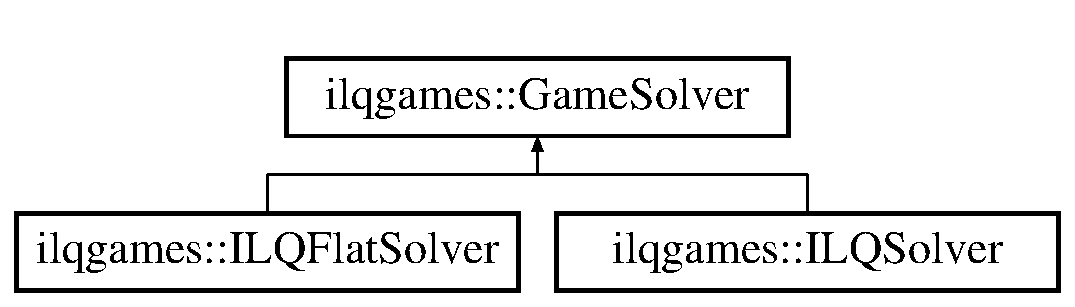
\includegraphics[height=2.000000cm]{classilqgames_1_1_game_solver}
\end{center}
\end{figure}
\subsection*{Public Member Functions}
\begin{DoxyCompactItemize}
\item 
virtual bool {\bfseries Solve} (const Vector\+Xf \&x0, const \hyperlink{structilqgames_1_1_operating_point}{Operating\+Point} \&initial\+\_\+operating\+\_\+point, const std\+::vector$<$ \hyperlink{structilqgames_1_1_strategy}{Strategy} $>$ \&initial\+\_\+strategies, \hyperlink{structilqgames_1_1_operating_point}{Operating\+Point} $\ast$final\+\_\+operating\+\_\+point, std\+::vector$<$ \hyperlink{structilqgames_1_1_strategy}{Strategy} $>$ $\ast$final\+\_\+strategies, \hyperlink{classilqgames_1_1_solver_log}{Solver\+Log} $\ast$log=nullptr, Time max\+\_\+runtime=std\+::numeric\+\_\+limits$<$ Time $>$\+::infinity())\hypertarget{classilqgames_1_1_game_solver_a24ed8caa4c9217122f7ce86f16d1bd34}{}\label{classilqgames_1_1_game_solver_a24ed8caa4c9217122f7ce86f16d1bd34}

\item 
Time {\bfseries Time\+Horizon} () const \hypertarget{classilqgames_1_1_game_solver_a9fa5328990bd8139c556c09453020e33}{}\label{classilqgames_1_1_game_solver_a9fa5328990bd8139c556c09453020e33}

\item 
size\+\_\+t {\bfseries Num\+Time\+Steps} () const \hypertarget{classilqgames_1_1_game_solver_a8234f72d8ee55b7afe4d3557e2c9e117}{}\label{classilqgames_1_1_game_solver_a8234f72d8ee55b7afe4d3557e2c9e117}

\item 
Time {\bfseries Time\+Step} () const \hypertarget{classilqgames_1_1_game_solver_a113252da6aa43d0beb9966277653af04}{}\label{classilqgames_1_1_game_solver_a113252da6aa43d0beb9966277653af04}

\item 
const std\+::vector$<$ \hyperlink{classilqgames_1_1_player_cost}{Player\+Cost} $>$ \& {\bfseries Player\+Costs} () const \hypertarget{classilqgames_1_1_game_solver_afe05eb1238b481b82747f9edf005c301}{}\label{classilqgames_1_1_game_solver_afe05eb1238b481b82747f9edf005c301}

\item 
const \hyperlink{classilqgames_1_1_multi_player_integrable_system}{Multi\+Player\+Integrable\+System} \& {\bfseries Dynamics} () const \hypertarget{classilqgames_1_1_game_solver_aa0917153345988be1661fca76a6f8500}{}\label{classilqgames_1_1_game_solver_aa0917153345988be1661fca76a6f8500}

\item 
Time {\bfseries Compute\+Time\+Stamp} (size\+\_\+t time\+\_\+index) const \hypertarget{classilqgames_1_1_game_solver_a490b20711d5d698171620f5bce607027}{}\label{classilqgames_1_1_game_solver_a490b20711d5d698171620f5bce607027}

\end{DoxyCompactItemize}
\subsection*{Protected Member Functions}
\begin{DoxyCompactItemize}
\item 
{\bfseries Game\+Solver} (const std\+::shared\+\_\+ptr$<$ const \hyperlink{classilqgames_1_1_multi_player_integrable_system}{Multi\+Player\+Integrable\+System} $>$ \&dynamics, const std\+::vector$<$ \hyperlink{classilqgames_1_1_player_cost}{Player\+Cost} $>$ \&player\+\_\+costs, Time time\+\_\+horizon, const \hyperlink{structilqgames_1_1_solver_params}{Solver\+Params} \&params=\hyperlink{structilqgames_1_1_solver_params}{Solver\+Params}())\hypertarget{classilqgames_1_1_game_solver_a89a591bb5d9fcefc28157a54b016a4d1}{}\label{classilqgames_1_1_game_solver_a89a591bb5d9fcefc28157a54b016a4d1}

\item 
virtual void {\bfseries Compute\+Linearization} (const \hyperlink{structilqgames_1_1_operating_point}{Operating\+Point} \&op, std\+::vector$<$ \hyperlink{structilqgames_1_1_linear_dynamics_approximation}{Linear\+Dynamics\+Approximation} $>$ $\ast$linearization)=0\hypertarget{classilqgames_1_1_game_solver_a4a1772a9bd07347ed28455119b2571fe}{}\label{classilqgames_1_1_game_solver_a4a1772a9bd07347ed28455119b2571fe}

\item 
virtual bool {\bfseries Modify\+L\+Q\+Strategies} (std\+::vector$<$ \hyperlink{structilqgames_1_1_strategy}{Strategy} $>$ $\ast$strategies, \hyperlink{structilqgames_1_1_operating_point}{Operating\+Point} $\ast$current\+\_\+operating\+\_\+point, bool $\ast$has\+\_\+converged, bool $\ast$was\+\_\+initial\+\_\+point\+\_\+feasible, std\+::vector$<$ float $>$ $\ast$total\+\_\+costs) const \hypertarget{classilqgames_1_1_game_solver_abb3f6d9e9facd9671d4c37f852c20aea}{}\label{classilqgames_1_1_game_solver_abb3f6d9e9facd9671d4c37f852c20aea}

\item 
virtual float {\bfseries State\+Distance} (const Vector\+Xf \&x1, const Vector\+Xf \&x2, const std\+::vector$<$ Dimension $>$ \&dims) const \hypertarget{classilqgames_1_1_game_solver_a413329f89a63805c387e35a99b53ad73}{}\label{classilqgames_1_1_game_solver_a413329f89a63805c387e35a99b53ad73}

\item 
bool {\bfseries Current\+Operating\+Point} (const \hyperlink{structilqgames_1_1_operating_point}{Operating\+Point} \&last\+\_\+operating\+\_\+point, const std\+::vector$<$ \hyperlink{structilqgames_1_1_strategy}{Strategy} $>$ \&current\+\_\+strategies, \hyperlink{structilqgames_1_1_operating_point}{Operating\+Point} $\ast$current\+\_\+operating\+\_\+point, bool $\ast$has\+\_\+converged, std\+::vector$<$ float $>$ $\ast$total\+\_\+costs, bool check\+\_\+trust\+\_\+region=true) const \hypertarget{classilqgames_1_1_game_solver_aec793cd5afb9cf01102fb2c5d852d186}{}\label{classilqgames_1_1_game_solver_aec793cd5afb9cf01102fb2c5d852d186}

\end{DoxyCompactItemize}
\subsection*{Protected Attributes}
\begin{DoxyCompactItemize}
\item 
const std\+::shared\+\_\+ptr$<$ const \hyperlink{classilqgames_1_1_multi_player_integrable_system}{Multi\+Player\+Integrable\+System} $>$ {\bfseries dynamics\+\_\+}\hypertarget{classilqgames_1_1_game_solver_addd321f0c2c7a760bccd2e4f043b3725}{}\label{classilqgames_1_1_game_solver_addd321f0c2c7a760bccd2e4f043b3725}

\item 
std\+::vector$<$ \hyperlink{classilqgames_1_1_player_cost}{Player\+Cost} $>$ {\bfseries player\+\_\+costs\+\_\+}\hypertarget{classilqgames_1_1_game_solver_aa9271829f762e9ad732921042005f856}{}\label{classilqgames_1_1_game_solver_aa9271829f762e9ad732921042005f856}

\item 
const Time {\bfseries time\+\_\+horizon\+\_\+}\hypertarget{classilqgames_1_1_game_solver_ae515fafef0ee7df96cfe1447d9f35581}{}\label{classilqgames_1_1_game_solver_ae515fafef0ee7df96cfe1447d9f35581}

\item 
const Time {\bfseries time\+\_\+step\+\_\+}\hypertarget{classilqgames_1_1_game_solver_ae1e0efeb25072ac9f21699b82071c6ab}{}\label{classilqgames_1_1_game_solver_ae1e0efeb25072ac9f21699b82071c6ab}

\item 
const size\+\_\+t {\bfseries num\+\_\+time\+\_\+steps\+\_\+}\hypertarget{classilqgames_1_1_game_solver_a8a95abeb47770462608d2f34b97c974e}{}\label{classilqgames_1_1_game_solver_a8a95abeb47770462608d2f34b97c974e}

\item 
std\+::vector$<$ \hyperlink{structilqgames_1_1_linear_dynamics_approximation}{Linear\+Dynamics\+Approximation} $>$ {\bfseries linearization\+\_\+}\hypertarget{classilqgames_1_1_game_solver_ad31cd30bf0b2fd95461672da928e91f2}{}\label{classilqgames_1_1_game_solver_ad31cd30bf0b2fd95461672da928e91f2}

\item 
std\+::vector$<$ std\+::vector$<$ \hyperlink{structilqgames_1_1_quadratic_cost_approximation}{Quadratic\+Cost\+Approximation} $>$ $>$ {\bfseries quadraticization\+\_\+}\hypertarget{classilqgames_1_1_game_solver_a039a0b26778f15ce89509452b11c5fb2}{}\label{classilqgames_1_1_game_solver_a039a0b26778f15ce89509452b11c5fb2}

\item 
std\+::unique\+\_\+ptr$<$ \hyperlink{classilqgames_1_1_l_q_solver}{L\+Q\+Solver} $>$ {\bfseries lq\+\_\+solver\+\_\+}\hypertarget{classilqgames_1_1_game_solver_a1b7e0da6a2566c0a959b7c6c9d7845be}{}\label{classilqgames_1_1_game_solver_a1b7e0da6a2566c0a959b7c6c9d7845be}

\item 
const \hyperlink{structilqgames_1_1_solver_params}{Solver\+Params} {\bfseries params\+\_\+}\hypertarget{classilqgames_1_1_game_solver_adb70fc48a6420c1b516becd5c108a92a}{}\label{classilqgames_1_1_game_solver_adb70fc48a6420c1b516becd5c108a92a}

\item 
\hyperlink{classilqgames_1_1_loop_timer}{Loop\+Timer} {\bfseries timer\+\_\+}\hypertarget{classilqgames_1_1_game_solver_ae77a0725fdd98ec49f96ebf33d966650}{}\label{classilqgames_1_1_game_solver_ae77a0725fdd98ec49f96ebf33d966650}

\end{DoxyCompactItemize}


\subsection{Detailed Description}


Definition at line 80 of file game\+\_\+solver.\+h.



The documentation for this class was generated from the following files\+:\begin{DoxyCompactItemize}
\item 
/home/travis/build/\+H\+J\+Reachability/ilqgames/include/ilqgames/solver/game\+\_\+solver.\+h\item 
/home/travis/build/\+H\+J\+Reachability/ilqgames/src/game\+\_\+solver.\+cpp\end{DoxyCompactItemize}

\hypertarget{classilqgames_1_1_i_l_q_flat_solver}{}\section{ilqgames\+:\+:I\+L\+Q\+Flat\+Solver Class Reference}
\label{classilqgames_1_1_i_l_q_flat_solver}\index{ilqgames\+::\+I\+L\+Q\+Flat\+Solver@{ilqgames\+::\+I\+L\+Q\+Flat\+Solver}}
Inheritance diagram for ilqgames\+:\+:I\+L\+Q\+Flat\+Solver\+:\begin{figure}[H]
\begin{center}
\leavevmode
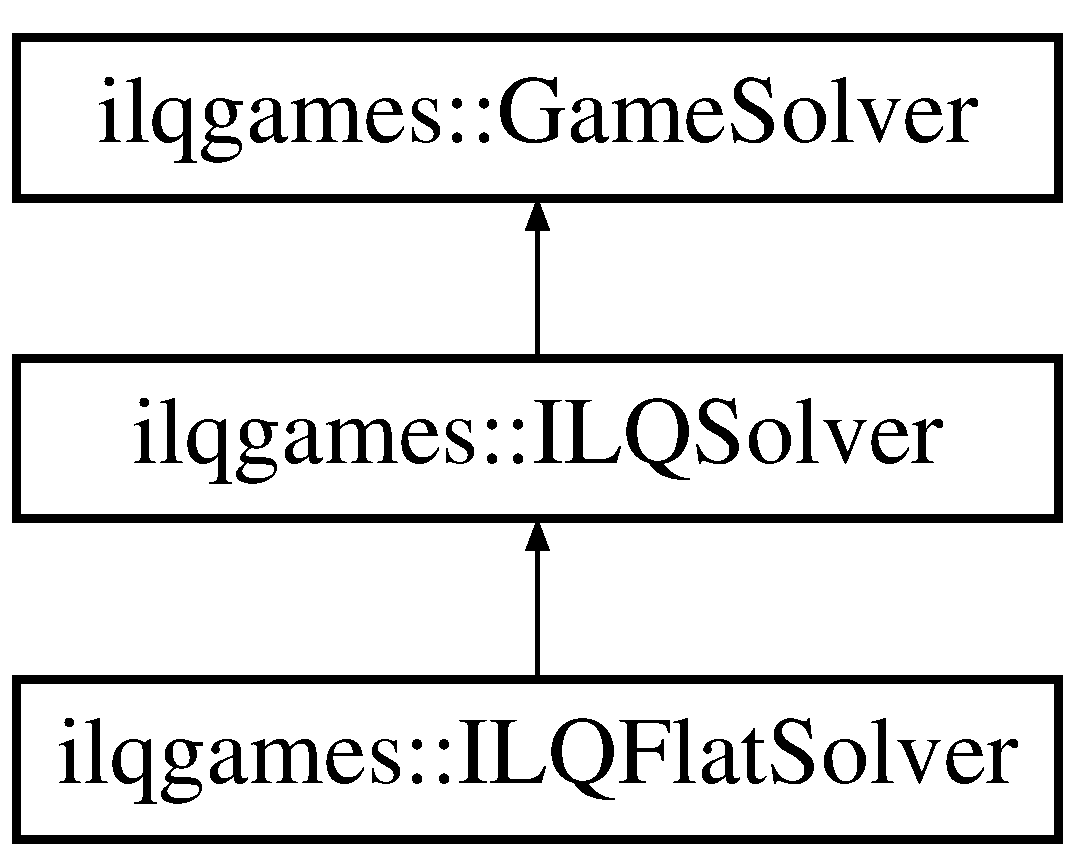
\includegraphics[height=2.000000cm]{classilqgames_1_1_i_l_q_flat_solver}
\end{center}
\end{figure}
\subsection*{Public Member Functions}
\begin{DoxyCompactItemize}
\item 
{\bfseries I\+L\+Q\+Flat\+Solver} (const std\+::shared\+\_\+ptr$<$ const \hyperlink{classilqgames_1_1_multi_player_flat_system}{Multi\+Player\+Flat\+System} $>$ \&dynamics, const std\+::vector$<$ \hyperlink{classilqgames_1_1_player_cost}{Player\+Cost} $>$ \&player\+\_\+costs, Time time\+\_\+horizon, const \hyperlink{structilqgames_1_1_solver_params}{Solver\+Params} \&params=\hyperlink{structilqgames_1_1_solver_params}{Solver\+Params}())\hypertarget{classilqgames_1_1_i_l_q_flat_solver_a66d3b8710861b90c67ea854b4722b2a2}{}\label{classilqgames_1_1_i_l_q_flat_solver_a66d3b8710861b90c67ea854b4722b2a2}

\item 
bool {\bfseries Solve} (const Vector\+Xf \&xi0, const \hyperlink{structilqgames_1_1_operating_point}{Operating\+Point} \&initial\+\_\+operating\+\_\+point, const std\+::vector$<$ \hyperlink{structilqgames_1_1_strategy}{Strategy} $>$ \&initial\+\_\+strategies, \hyperlink{structilqgames_1_1_operating_point}{Operating\+Point} $\ast$final\+\_\+operating\+\_\+point, std\+::vector$<$ \hyperlink{structilqgames_1_1_strategy}{Strategy} $>$ $\ast$final\+\_\+strategies, \hyperlink{classilqgames_1_1_solver_log}{Solver\+Log} $\ast$log=nullptr, Time max\+\_\+runtime=std\+::numeric\+\_\+limits$<$ Time $>$\+::infinity())\hypertarget{classilqgames_1_1_i_l_q_flat_solver_a1229821b72869b3031d51a1afbb34eb2}{}\label{classilqgames_1_1_i_l_q_flat_solver_a1229821b72869b3031d51a1afbb34eb2}

\end{DoxyCompactItemize}
\subsection*{Protected Member Functions}
\begin{DoxyCompactItemize}
\item 
virtual bool {\bfseries Satisfies\+Trust\+Region} (const \hyperlink{structilqgames_1_1_operating_point}{Operating\+Point} \&last\+\_\+operating\+\_\+point, const \hyperlink{structilqgames_1_1_operating_point}{Operating\+Point} \&current\+\_\+operating\+\_\+point) const \hypertarget{classilqgames_1_1_i_l_q_flat_solver_a0f9a32d7bb55ff8d44c6a34ecc2335ee}{}\label{classilqgames_1_1_i_l_q_flat_solver_a0f9a32d7bb55ff8d44c6a34ecc2335ee}

\item 
virtual bool {\bfseries Are\+Operating\+Points\+Close} (const \hyperlink{structilqgames_1_1_operating_point}{Operating\+Point} \&op1, const \hyperlink{structilqgames_1_1_operating_point}{Operating\+Point} \&op2, float threshold, const std\+::vector$<$ Dimension $>$ \&dims) const \hypertarget{classilqgames_1_1_i_l_q_flat_solver_a4b79c70958d7ac9eb19c8b95de8dc33a}{}\label{classilqgames_1_1_i_l_q_flat_solver_a4b79c70958d7ac9eb19c8b95de8dc33a}

\end{DoxyCompactItemize}
\subsection*{Additional Inherited Members}


\subsection{Detailed Description}


Definition at line 65 of file ilq\+\_\+flat\+\_\+solver.\+h.



The documentation for this class was generated from the following files\+:\begin{DoxyCompactItemize}
\item 
/home/travis/build/\+H\+J\+Reachability/ilqgames/include/ilqgames/solver/ilq\+\_\+flat\+\_\+solver.\+h\item 
/home/travis/build/\+H\+J\+Reachability/ilqgames/src/ilq\+\_\+flat\+\_\+solver.\+cpp\end{DoxyCompactItemize}

\hypertarget{classilqgames_1_1_i_l_q_solver}{}\section{ilqgames\+:\+:I\+L\+Q\+Solver Class Reference}
\label{classilqgames_1_1_i_l_q_solver}\index{ilqgames\+::\+I\+L\+Q\+Solver@{ilqgames\+::\+I\+L\+Q\+Solver}}
Inheritance diagram for ilqgames\+:\+:I\+L\+Q\+Solver\+:\begin{figure}[H]
\begin{center}
\leavevmode
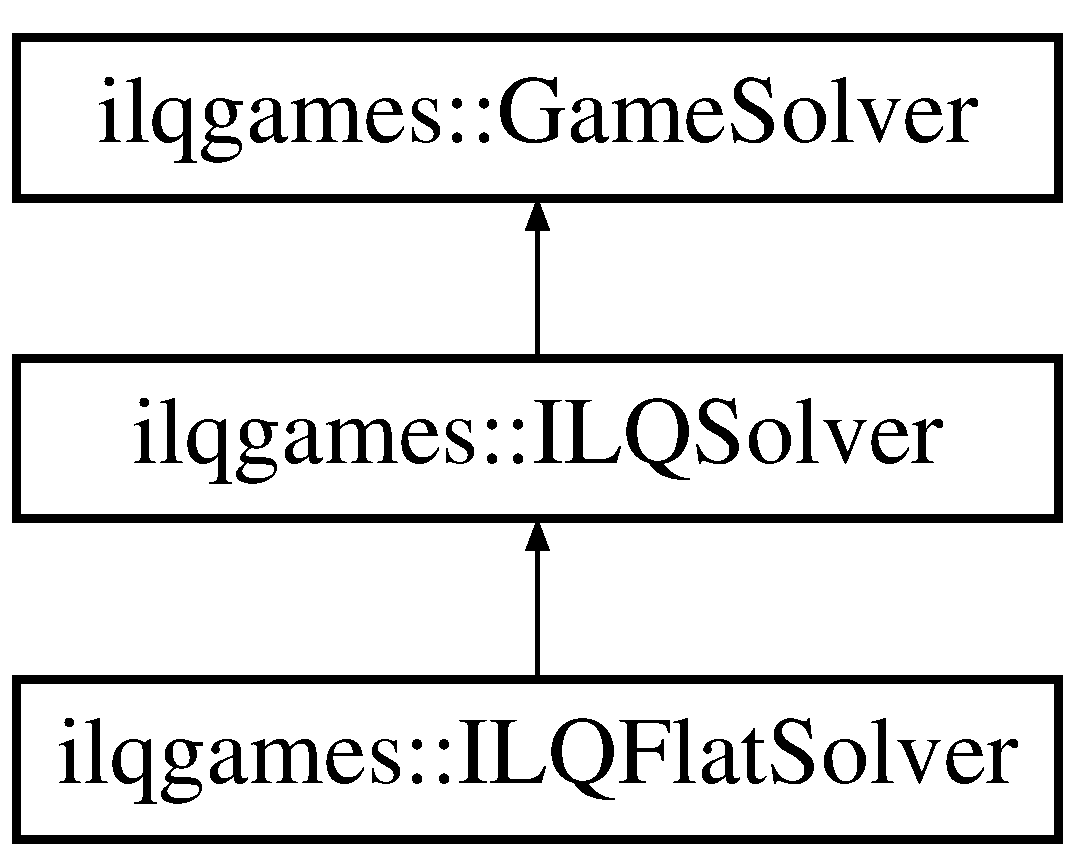
\includegraphics[height=3.000000cm]{classilqgames_1_1_i_l_q_solver}
\end{center}
\end{figure}
\subsection*{Public Member Functions}
\begin{DoxyCompactItemize}
\item 
{\bfseries I\+L\+Q\+Solver} (const std\+::shared\+\_\+ptr$<$ \hyperlink{classilqgames_1_1_problem}{Problem} $>$ \&problem, const \hyperlink{structilqgames_1_1_solver_params}{Solver\+Params} \&params=\hyperlink{structilqgames_1_1_solver_params}{Solver\+Params}())\hypertarget{classilqgames_1_1_i_l_q_solver_a873b090b6a55ce1c33f780942c51e464}{}\label{classilqgames_1_1_i_l_q_solver_a873b090b6a55ce1c33f780942c51e464}

\item 
virtual std\+::shared\+\_\+ptr$<$ \hyperlink{classilqgames_1_1_solver_log}{Solver\+Log} $>$ {\bfseries Solve} (bool $\ast$success=nullptr, Time max\+\_\+runtime=std\+::numeric\+\_\+limits$<$ Time $>$\+::infinity())\hypertarget{classilqgames_1_1_i_l_q_solver_ad86d47ce8a04ab5f8e8fcfbf3db6b02e}{}\label{classilqgames_1_1_i_l_q_solver_ad86d47ce8a04ab5f8e8fcfbf3db6b02e}

\end{DoxyCompactItemize}
\subsection*{Protected Member Functions}
\begin{DoxyCompactItemize}
\item 
bool {\bfseries Modify\+L\+Q\+Strategies} (std\+::vector$<$ \hyperlink{structilqgames_1_1_strategy}{Strategy} $>$ $\ast$strategies, \hyperlink{structilqgames_1_1_operating_point}{Operating\+Point} $\ast$current\+\_\+operating\+\_\+point, bool $\ast$is\+\_\+new\+\_\+operating\+\_\+point\+\_\+feasible)\hypertarget{classilqgames_1_1_i_l_q_solver_ada2e91b02b1e88947540dc3f9bbae7f0}{}\label{classilqgames_1_1_i_l_q_solver_ada2e91b02b1e88947540dc3f9bbae7f0}

\item 
virtual float {\bfseries State\+Distance} (const Vector\+Xf \&x1, const Vector\+Xf \&x2, const std\+::vector$<$ Dimension $>$ \&dims) const \hypertarget{classilqgames_1_1_i_l_q_solver_aee7f2cfccde0664200d62f92ed5e0606}{}\label{classilqgames_1_1_i_l_q_solver_aee7f2cfccde0664200d62f92ed5e0606}

\item 
virtual bool {\bfseries Has\+Converged} (const \hyperlink{structilqgames_1_1_operating_point}{Operating\+Point} \&last\+\_\+op, const \hyperlink{structilqgames_1_1_operating_point}{Operating\+Point} \&current\+\_\+op) const \hypertarget{classilqgames_1_1_i_l_q_solver_a16009dd589014a579b8b8ec5cbe89e87}{}\label{classilqgames_1_1_i_l_q_solver_a16009dd589014a579b8b8ec5cbe89e87}

\item 
void {\bfseries Total\+Costs} (const \hyperlink{structilqgames_1_1_operating_point}{Operating\+Point} \&current\+\_\+op, std\+::vector$<$ float $>$ $\ast$total\+\_\+costs) const \hypertarget{classilqgames_1_1_i_l_q_solver_acf0f45f07d5484a9a60b3a2e1db1647a}{}\label{classilqgames_1_1_i_l_q_solver_acf0f45f07d5484a9a60b3a2e1db1647a}

\item 
bool {\bfseries Check\+Armijo\+Condition} (const \hyperlink{structilqgames_1_1_operating_point}{Operating\+Point} \&current\+\_\+op, float current\+\_\+stepsize, float $\ast$current\+\_\+kkt\+\_\+squared\+\_\+error)\hypertarget{classilqgames_1_1_i_l_q_solver_a4e7525bb720f83e255dac165f0bbeb57}{}\label{classilqgames_1_1_i_l_q_solver_a4e7525bb720f83e255dac165f0bbeb57}

\item 
float {\bfseries K\+K\+T\+Squared\+Error} (const \hyperlink{structilqgames_1_1_operating_point}{Operating\+Point} \&current\+\_\+op)\hypertarget{classilqgames_1_1_i_l_q_solver_a9845b60307967eca6aa6897897d5ee69}{}\label{classilqgames_1_1_i_l_q_solver_a9845b60307967eca6aa6897897d5ee69}

\item 
void {\bfseries Current\+Operating\+Point} (const \hyperlink{structilqgames_1_1_operating_point}{Operating\+Point} \&last\+\_\+operating\+\_\+point, const std\+::vector$<$ \hyperlink{structilqgames_1_1_strategy}{Strategy} $>$ \&current\+\_\+strategies, \hyperlink{structilqgames_1_1_operating_point}{Operating\+Point} $\ast$current\+\_\+operating\+\_\+point, bool $\ast$satisfies\+\_\+barriers=nullptr) const \hypertarget{classilqgames_1_1_i_l_q_solver_ae5dd6b941a6caa2091547e27b7ca8869}{}\label{classilqgames_1_1_i_l_q_solver_ae5dd6b941a6caa2091547e27b7ca8869}

\end{DoxyCompactItemize}
\subsection*{Protected Attributes}
\begin{DoxyCompactItemize}
\item 
std\+::unique\+\_\+ptr$<$ \hyperlink{classilqgames_1_1_l_q_solver}{L\+Q\+Solver} $>$ {\bfseries lq\+\_\+solver\+\_\+}\hypertarget{classilqgames_1_1_i_l_q_solver_afb4b2fed2450e965d347dd6a38a33bb6}{}\label{classilqgames_1_1_i_l_q_solver_afb4b2fed2450e965d347dd6a38a33bb6}

\item 
float {\bfseries last\+\_\+kkt\+\_\+squared\+\_\+error\+\_\+}\hypertarget{classilqgames_1_1_i_l_q_solver_aad3c6e1b11d4c17ff63d87b3755c11b9}{}\label{classilqgames_1_1_i_l_q_solver_aad3c6e1b11d4c17ff63d87b3755c11b9}

\item 
std\+::unique\+\_\+ptr$<$ float $>$ {\bfseries expected\+\_\+decrease\+\_\+}\hypertarget{classilqgames_1_1_i_l_q_solver_a58f9f117f6c03931c46d4ccece3386c7}{}\label{classilqgames_1_1_i_l_q_solver_a58f9f117f6c03931c46d4ccece3386c7}

\end{DoxyCompactItemize}


\subsection{Detailed Description}


Definition at line 66 of file ilq\+\_\+solver.\+h.



The documentation for this class was generated from the following files\+:\begin{DoxyCompactItemize}
\item 
/home/travis/build/\+H\+J\+Reachability/ilqgames/include/ilqgames/solver/ilq\+\_\+solver.\+h\item 
/home/travis/build/\+H\+J\+Reachability/ilqgames/src/ilq\+\_\+solver.\+cpp\end{DoxyCompactItemize}

\hypertarget{structilqgames_1_1_linear_dynamics_approximation}{}\section{ilqgames\+:\+:Linear\+Dynamics\+Approximation Struct Reference}
\label{structilqgames_1_1_linear_dynamics_approximation}\index{ilqgames\+::\+Linear\+Dynamics\+Approximation@{ilqgames\+::\+Linear\+Dynamics\+Approximation}}
\subsection*{Public Member Functions}
\begin{DoxyCompactItemize}
\item 
{\footnotesize template$<$typename Multi\+Player\+System\+Type $>$ }\\{\bfseries Linear\+Dynamics\+Approximation} (const Multi\+Player\+System\+Type \&system)\hypertarget{structilqgames_1_1_linear_dynamics_approximation_aa9006868bfdb5e6f9160ddb5758c42aa}{}\label{structilqgames_1_1_linear_dynamics_approximation_aa9006868bfdb5e6f9160ddb5758c42aa}

\end{DoxyCompactItemize}
\subsection*{Public Attributes}
\begin{DoxyCompactItemize}
\item 
Matrix\+Xf {\bfseries A}\hypertarget{structilqgames_1_1_linear_dynamics_approximation_a2587c5e802fe56485192dadd90203a7c}{}\label{structilqgames_1_1_linear_dynamics_approximation_a2587c5e802fe56485192dadd90203a7c}

\item 
std\+::vector$<$ Matrix\+Xf $>$ {\bfseries Bs}\hypertarget{structilqgames_1_1_linear_dynamics_approximation_ac57ed8a24e467da727811fe4251e5c72}{}\label{structilqgames_1_1_linear_dynamics_approximation_ac57ed8a24e467da727811fe4251e5c72}

\end{DoxyCompactItemize}


\subsection{Detailed Description}


Definition at line 53 of file linear\+\_\+dynamics\+\_\+approximation.\+h.



The documentation for this struct was generated from the following file\+:\begin{DoxyCompactItemize}
\item 
/home/travis/build/\+H\+J\+Reachability/ilqgames/include/ilqgames/utils/linear\+\_\+dynamics\+\_\+approximation.\+h\end{DoxyCompactItemize}

\hypertarget{classilqgames_1_1_line_segment2}{}\section{ilqgames\+:\+:Line\+Segment2 Class Reference}
\label{classilqgames_1_1_line_segment2}\index{ilqgames\+::\+Line\+Segment2@{ilqgames\+::\+Line\+Segment2}}
\subsection*{Public Member Functions}
\begin{DoxyCompactItemize}
\item 
{\bfseries Line\+Segment2} (const Point2 \&point1, const Point2 \&point2)\hypertarget{classilqgames_1_1_line_segment2_a364902f44220f68ea07588641a6778fd}{}\label{classilqgames_1_1_line_segment2_a364902f44220f68ea07588641a6778fd}

\item 
float {\bfseries Length} () const \hypertarget{classilqgames_1_1_line_segment2_a4458797af59ef84bd7ef875a1db3ff14}{}\label{classilqgames_1_1_line_segment2_a4458797af59ef84bd7ef875a1db3ff14}

\item 
const Point2 \& {\bfseries First\+Point} () const \hypertarget{classilqgames_1_1_line_segment2_a1374aed3332613dd7790b4f5dfa4d710}{}\label{classilqgames_1_1_line_segment2_a1374aed3332613dd7790b4f5dfa4d710}

\item 
const Point2 \& {\bfseries Second\+Point} () const \hypertarget{classilqgames_1_1_line_segment2_a513513fbd19254698a2f87fa6f650560}{}\label{classilqgames_1_1_line_segment2_a513513fbd19254698a2f87fa6f650560}

\item 
const Point2 \& {\bfseries Unit\+Direction} () const \hypertarget{classilqgames_1_1_line_segment2_a59a4eb9563be4a49d64deee301f4be6b}{}\label{classilqgames_1_1_line_segment2_a59a4eb9563be4a49d64deee301f4be6b}

\item 
float {\bfseries Heading} () const \hypertarget{classilqgames_1_1_line_segment2_a5a11245e7e612d222795f03e68eb31c1}{}\label{classilqgames_1_1_line_segment2_a5a11245e7e612d222795f03e68eb31c1}

\item 
bool {\bfseries Side} (const Point2 \&query) const \hypertarget{classilqgames_1_1_line_segment2_a788a9936c769a6664b824614e4f7d764}{}\label{classilqgames_1_1_line_segment2_a788a9936c769a6664b824614e4f7d764}

\item 
Point2 {\bfseries Closest\+Point} (const Point2 \&query, bool $\ast$is\+\_\+endpoint=nullptr, float $\ast$signed\+\_\+squared\+\_\+distance=nullptr) const \hypertarget{classilqgames_1_1_line_segment2_a13944bbafcdae15692706c0859b5d3d5}{}\label{classilqgames_1_1_line_segment2_a13944bbafcdae15692706c0859b5d3d5}

\end{DoxyCompactItemize}


\subsection{Detailed Description}


Definition at line 52 of file line\+\_\+segment2.\+h.



The documentation for this class was generated from the following files\+:\begin{DoxyCompactItemize}
\item 
/home/travis/build/\+H\+J\+Reachability/ilqgames/include/ilqgames/geometry/line\+\_\+segment2.\+h\item 
/home/travis/build/\+H\+J\+Reachability/ilqgames/src/line\+\_\+segment2.\+cpp\end{DoxyCompactItemize}

\hypertarget{classilqgames_1_1_locally_convex_proximity_cost}{}\section{ilqgames\+:\+:Locally\+Convex\+Proximity\+Cost Class Reference}
\label{classilqgames_1_1_locally_convex_proximity_cost}\index{ilqgames\+::\+Locally\+Convex\+Proximity\+Cost@{ilqgames\+::\+Locally\+Convex\+Proximity\+Cost}}
Inheritance diagram for ilqgames\+:\+:Locally\+Convex\+Proximity\+Cost\+:\begin{figure}[H]
\begin{center}
\leavevmode
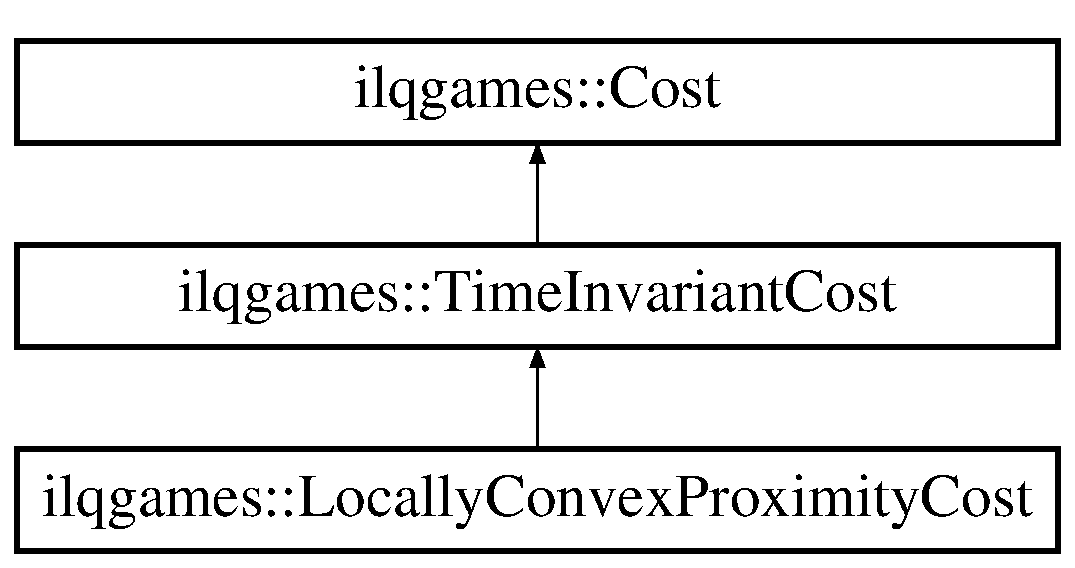
\includegraphics[height=3.000000cm]{classilqgames_1_1_locally_convex_proximity_cost}
\end{center}
\end{figure}
\subsection*{Public Member Functions}
\begin{DoxyCompactItemize}
\item 
{\bfseries Locally\+Convex\+Proximity\+Cost} (float weight, const std\+::pair$<$ Dimension, Dimension $>$ \&position\+\_\+idxs1, const std\+::pair$<$ Dimension, Dimension $>$ \&position\+\_\+idxs2, float threshold, const std\+::string \&name=\char`\"{}\char`\"{})\hypertarget{classilqgames_1_1_locally_convex_proximity_cost_aabea3cea381b56639bcb4e60df93ee48}{}\label{classilqgames_1_1_locally_convex_proximity_cost_aabea3cea381b56639bcb4e60df93ee48}

\item 
float {\bfseries Evaluate} (const Vector\+Xf \&input) const \hypertarget{classilqgames_1_1_locally_convex_proximity_cost_ae0f309dfa69dc2c46158afda394af9e3}{}\label{classilqgames_1_1_locally_convex_proximity_cost_ae0f309dfa69dc2c46158afda394af9e3}

\item 
void {\bfseries Quadraticize} (const Vector\+Xf \&input, Matrix\+Xf $\ast$hess, Vector\+Xf $\ast$grad) const \hypertarget{classilqgames_1_1_locally_convex_proximity_cost_adf826e1e1063bad897a5dcce3c3bc44c}{}\label{classilqgames_1_1_locally_convex_proximity_cost_adf826e1e1063bad897a5dcce3c3bc44c}

\end{DoxyCompactItemize}
\subsection*{Additional Inherited Members}


\subsection{Detailed Description}


Definition at line 54 of file locally\+\_\+convex\+\_\+proximity\+\_\+cost.\+h.



The documentation for this class was generated from the following files\+:\begin{DoxyCompactItemize}
\item 
/home/travis/build/\+H\+J\+Reachability/ilqgames/include/ilqgames/cost/locally\+\_\+convex\+\_\+proximity\+\_\+cost.\+h\item 
/home/travis/build/\+H\+J\+Reachability/ilqgames/src/locally\+\_\+convex\+\_\+proximity\+\_\+cost.\+cpp\end{DoxyCompactItemize}

\hypertarget{classilqgames_1_1_loop_timer}{}\section{ilqgames\+:\+:Loop\+Timer Class Reference}
\label{classilqgames_1_1_loop_timer}\index{ilqgames\+::\+Loop\+Timer@{ilqgames\+::\+Loop\+Timer}}
\subsection*{Public Member Functions}
\begin{DoxyCompactItemize}
\item 
{\bfseries Loop\+Timer} (size\+\_\+t max\+\_\+samples=10)\hypertarget{classilqgames_1_1_loop_timer_adf0fca5ddad39e3939fc178b698b3e4d}{}\label{classilqgames_1_1_loop_timer_adf0fca5ddad39e3939fc178b698b3e4d}

\item 
void {\bfseries Tic} ()\hypertarget{classilqgames_1_1_loop_timer_aa4bdb7d7b8550356ffd177890c11c8ef}{}\label{classilqgames_1_1_loop_timer_aa4bdb7d7b8550356ffd177890c11c8ef}

\item 
Time {\bfseries Toc} ()\hypertarget{classilqgames_1_1_loop_timer_a9361224acb6b77b1e6546f3e76625fe2}{}\label{classilqgames_1_1_loop_timer_a9361224acb6b77b1e6546f3e76625fe2}

\item 
Time {\bfseries Runtime\+Upper\+Bound} (float num\+\_\+stddevs=3.\+0, Time initial\+\_\+guess=0.\+02) const \hypertarget{classilqgames_1_1_loop_timer_a551691bad650b5c70efbeb08b355638f}{}\label{classilqgames_1_1_loop_timer_a551691bad650b5c70efbeb08b355638f}

\end{DoxyCompactItemize}


\subsection{Detailed Description}


Definition at line 57 of file loop\+\_\+timer.\+h.



The documentation for this class was generated from the following files\+:\begin{DoxyCompactItemize}
\item 
/home/travis/build/\+H\+J\+Reachability/ilqgames/include/ilqgames/utils/loop\+\_\+timer.\+h\item 
/home/travis/build/\+H\+J\+Reachability/ilqgames/src/loop\+\_\+timer.\+cpp\end{DoxyCompactItemize}

\hypertarget{classilqgames_1_1_l_q_feedback_solver}{}\section{ilqgames\+:\+:L\+Q\+Feedback\+Solver Class Reference}
\label{classilqgames_1_1_l_q_feedback_solver}\index{ilqgames\+::\+L\+Q\+Feedback\+Solver@{ilqgames\+::\+L\+Q\+Feedback\+Solver}}
Inheritance diagram for ilqgames\+:\+:L\+Q\+Feedback\+Solver\+:\begin{figure}[H]
\begin{center}
\leavevmode
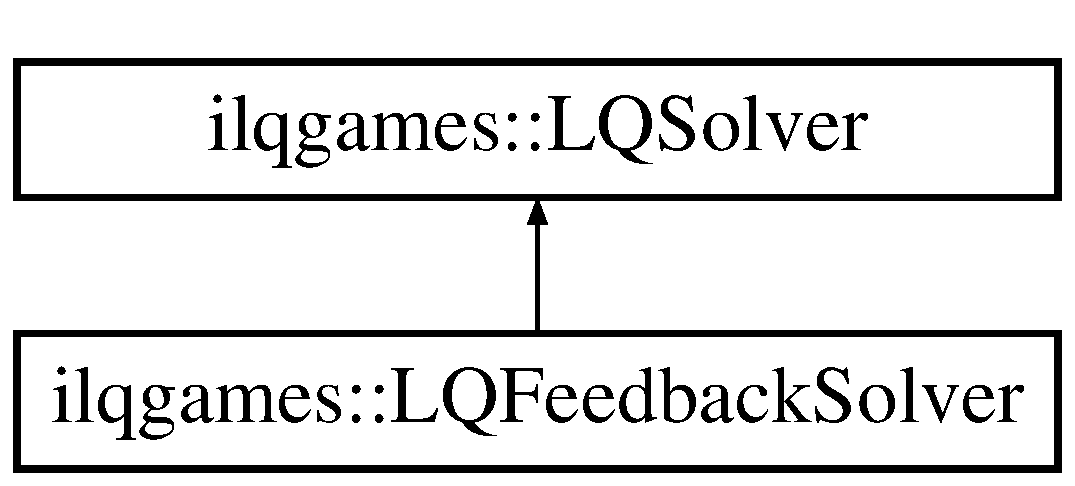
\includegraphics[height=2.000000cm]{classilqgames_1_1_l_q_feedback_solver}
\end{center}
\end{figure}
\subsection*{Public Member Functions}
\begin{DoxyCompactItemize}
\item 
{\bfseries L\+Q\+Feedback\+Solver} (const std\+::shared\+\_\+ptr$<$ const \hyperlink{classilqgames_1_1_multi_player_integrable_system}{Multi\+Player\+Integrable\+System} $>$ \&dynamics, size\+\_\+t num\+\_\+time\+\_\+steps)\hypertarget{classilqgames_1_1_l_q_feedback_solver_ac320229137060866f2020773657995ba}{}\label{classilqgames_1_1_l_q_feedback_solver_ac320229137060866f2020773657995ba}

\item 
std\+::vector$<$ \hyperlink{structilqgames_1_1_strategy}{Strategy} $>$ {\bfseries Solve} (const std\+::vector$<$ \hyperlink{structilqgames_1_1_linear_dynamics_approximation}{Linear\+Dynamics\+Approximation} $>$ \&linearization, const std\+::vector$<$ std\+::vector$<$ \hyperlink{structilqgames_1_1_quadratic_cost_approximation}{Quadratic\+Cost\+Approximation} $>$$>$ \&quadraticization, const Vector\+Xf \&x0, std\+::vector$<$ Vector\+Xf $>$ $\ast$delta\+\_\+xs=nullptr, std\+::vector$<$ std\+::vector$<$ Vector\+Xf $>$$>$ $\ast$costates=nullptr)\hypertarget{classilqgames_1_1_l_q_feedback_solver_ac48899856e1783291989e2c92d30ed36}{}\label{classilqgames_1_1_l_q_feedback_solver_ac48899856e1783291989e2c92d30ed36}

\end{DoxyCompactItemize}


\subsection{Detailed Description}


Definition at line 70 of file lq\+\_\+feedback\+\_\+solver.\+h.



The documentation for this class was generated from the following files\+:\begin{DoxyCompactItemize}
\item 
/home/travis/build/\+H\+J\+Reachability/ilqgames/include/ilqgames/solver/lq\+\_\+feedback\+\_\+solver.\+h\item 
/home/travis/build/\+H\+J\+Reachability/ilqgames/src/lq\+\_\+feedback\+\_\+solver.\+cpp\end{DoxyCompactItemize}

\hypertarget{classilqgames_1_1_l_q_open_loop_solver}{}\section{ilqgames\+:\+:L\+Q\+Open\+Loop\+Solver Class Reference}
\label{classilqgames_1_1_l_q_open_loop_solver}\index{ilqgames\+::\+L\+Q\+Open\+Loop\+Solver@{ilqgames\+::\+L\+Q\+Open\+Loop\+Solver}}
Inheritance diagram for ilqgames\+:\+:L\+Q\+Open\+Loop\+Solver\+:\begin{figure}[H]
\begin{center}
\leavevmode
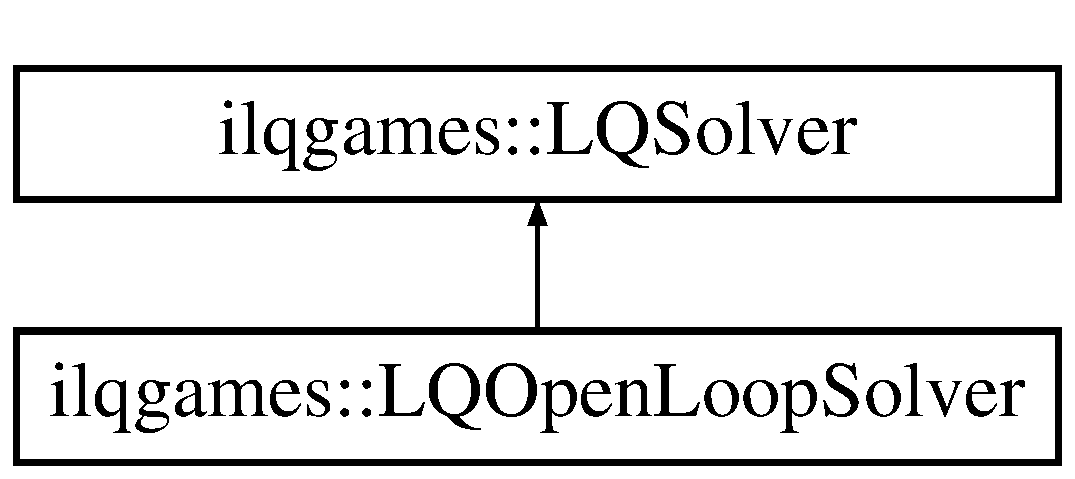
\includegraphics[height=2.000000cm]{classilqgames_1_1_l_q_open_loop_solver}
\end{center}
\end{figure}
\subsection*{Public Member Functions}
\begin{DoxyCompactItemize}
\item 
std\+::vector$<$ \hyperlink{structilqgames_1_1_strategy}{Strategy} $>$ {\bfseries Solve} (const \hyperlink{classilqgames_1_1_multi_player_integrable_system}{Multi\+Player\+Integrable\+System} \&dynamics, const std\+::vector$<$ \hyperlink{structilqgames_1_1_linear_dynamics_approximation}{Linear\+Dynamics\+Approximation} $>$ \&linearization, const std\+::vector$<$ std\+::vector$<$ \hyperlink{structilqgames_1_1_quadratic_cost_approximation}{Quadratic\+Cost\+Approximation} $>$$>$ \&quadraticization, const Vector\+Xf \&x0)\hypertarget{classilqgames_1_1_l_q_open_loop_solver_ad7d6f8df8329934d07ea7c2d1f30a4c6}{}\label{classilqgames_1_1_l_q_open_loop_solver_ad7d6f8df8329934d07ea7c2d1f30a4c6}

\end{DoxyCompactItemize}


\subsection{Detailed Description}


Definition at line 72 of file lq\+\_\+open\+\_\+loop\+\_\+solver.\+h.



The documentation for this class was generated from the following files\+:\begin{DoxyCompactItemize}
\item 
/home/travis/build/\+H\+J\+Reachability/ilqgames/include/ilqgames/solver/lq\+\_\+open\+\_\+loop\+\_\+solver.\+h\item 
/home/travis/build/\+H\+J\+Reachability/ilqgames/src/lq\+\_\+open\+\_\+loop\+\_\+solver.\+cpp\end{DoxyCompactItemize}

\hypertarget{classilqgames_1_1_l_q_solver}{}\section{ilqgames\+:\+:L\+Q\+Solver Class Reference}
\label{classilqgames_1_1_l_q_solver}\index{ilqgames\+::\+L\+Q\+Solver@{ilqgames\+::\+L\+Q\+Solver}}
Inheritance diagram for ilqgames\+:\+:L\+Q\+Solver\+:\begin{figure}[H]
\begin{center}
\leavevmode
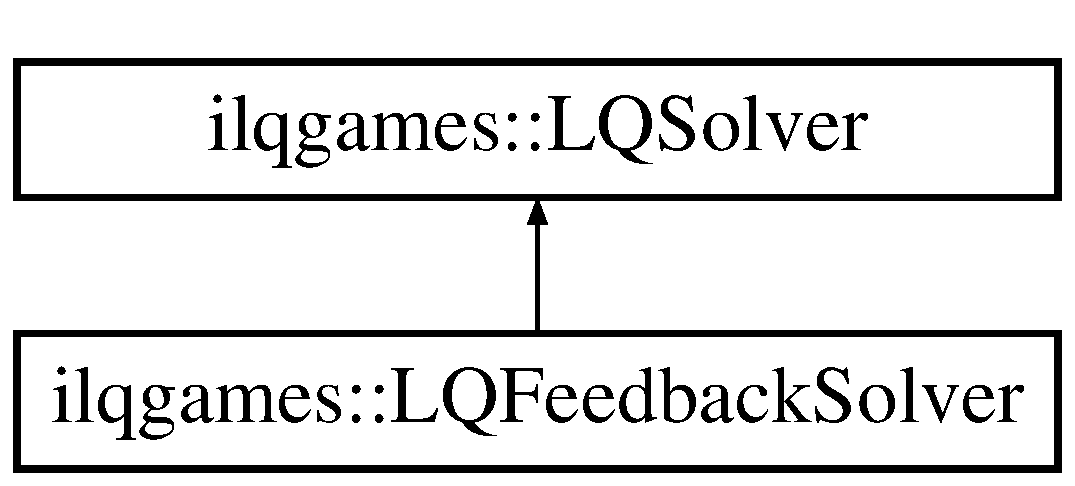
\includegraphics[height=1.996435cm]{classilqgames_1_1_l_q_solver}
\end{center}
\end{figure}
\subsection*{Public Member Functions}
\begin{DoxyCompactItemize}
\item 
virtual std\+::vector$<$ \hyperlink{structilqgames_1_1_strategy}{Strategy} $>$ {\bfseries Solve} (const std\+::vector$<$ \hyperlink{structilqgames_1_1_linear_dynamics_approximation}{Linear\+Dynamics\+Approximation} $>$ \&linearization, const std\+::vector$<$ std\+::vector$<$ \hyperlink{structilqgames_1_1_quadratic_cost_approximation}{Quadratic\+Cost\+Approximation} $>$$>$ \&quadraticization, const Vector\+Xf \&x0)=0\hypertarget{classilqgames_1_1_l_q_solver_ab40242e2a6e8f0749dfa3b9f450ebed0}{}\label{classilqgames_1_1_l_q_solver_ab40242e2a6e8f0749dfa3b9f450ebed0}

\end{DoxyCompactItemize}
\subsection*{Protected Member Functions}
\begin{DoxyCompactItemize}
\item 
{\bfseries L\+Q\+Solver} (const std\+::shared\+\_\+ptr$<$ const \hyperlink{classilqgames_1_1_multi_player_integrable_system}{Multi\+Player\+Integrable\+System} $>$ \&dynamics, size\+\_\+t num\+\_\+time\+\_\+steps)\hypertarget{classilqgames_1_1_l_q_solver_a0f96c7942e604bb26c68a48b2cb9dbc8}{}\label{classilqgames_1_1_l_q_solver_a0f96c7942e604bb26c68a48b2cb9dbc8}

\end{DoxyCompactItemize}
\subsection*{Protected Attributes}
\begin{DoxyCompactItemize}
\item 
const std\+::shared\+\_\+ptr$<$ const \hyperlink{classilqgames_1_1_multi_player_integrable_system}{Multi\+Player\+Integrable\+System} $>$ {\bfseries dynamics\+\_\+}\hypertarget{classilqgames_1_1_l_q_solver_a22c4249fdbf20669711fea2896e74fc5}{}\label{classilqgames_1_1_l_q_solver_a22c4249fdbf20669711fea2896e74fc5}

\item 
const size\+\_\+t {\bfseries num\+\_\+time\+\_\+steps\+\_\+}\hypertarget{classilqgames_1_1_l_q_solver_addcae93427e1ebc2dfa0f44d5dd88569}{}\label{classilqgames_1_1_l_q_solver_addcae93427e1ebc2dfa0f44d5dd88569}

\end{DoxyCompactItemize}


\subsection{Detailed Description}


Definition at line 57 of file lq\+\_\+solver.\+h.



The documentation for this class was generated from the following file\+:\begin{DoxyCompactItemize}
\item 
/home/travis/build/\+H\+J\+Reachability/ilqgames/include/ilqgames/solver/lq\+\_\+solver.\+h\end{DoxyCompactItemize}

\hypertarget{classilqgames_1_1_multi_player_dynamical_system}{}\section{ilqgames\+:\+:Multi\+Player\+Dynamical\+System Class Reference}
\label{classilqgames_1_1_multi_player_dynamical_system}\index{ilqgames\+::\+Multi\+Player\+Dynamical\+System@{ilqgames\+::\+Multi\+Player\+Dynamical\+System}}
Inheritance diagram for ilqgames\+:\+:Multi\+Player\+Dynamical\+System\+:\begin{figure}[H]
\begin{center}
\leavevmode
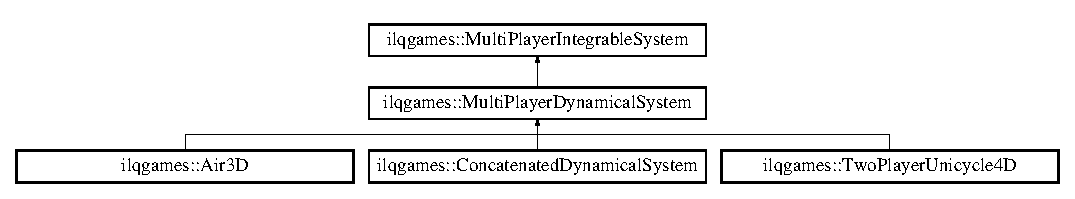
\includegraphics[height=3.000000cm]{classilqgames_1_1_multi_player_dynamical_system}
\end{center}
\end{figure}
\subsection*{Public Member Functions}
\begin{DoxyCompactItemize}
\item 
virtual Vector\+Xf {\bfseries Evaluate} (Time t, const Vector\+Xf \&x, const std\+::vector$<$ Vector\+Xf $>$ \&us) const =0\hypertarget{classilqgames_1_1_multi_player_dynamical_system_a66a5536c8b8995b26f1d5520026a6ad8}{}\label{classilqgames_1_1_multi_player_dynamical_system_a66a5536c8b8995b26f1d5520026a6ad8}

\item 
virtual \hyperlink{structilqgames_1_1_linear_dynamics_approximation}{Linear\+Dynamics\+Approximation} {\bfseries Linearize} (Time t, const Vector\+Xf \&x, const std\+::vector$<$ Vector\+Xf $>$ \&us) const =0\hypertarget{classilqgames_1_1_multi_player_dynamical_system_ace8dae90eae7aa2e0a327855f77c38d1}{}\label{classilqgames_1_1_multi_player_dynamical_system_ace8dae90eae7aa2e0a327855f77c38d1}

\item 
Vector\+Xf {\bfseries Integrate} (Time t0, Time time\+\_\+interval, const Vector\+Xf \&x0, const std\+::vector$<$ Vector\+Xf $>$ \&us) const \hypertarget{classilqgames_1_1_multi_player_dynamical_system_afddeafb94e74a19cdba2736f4a7a8050}{}\label{classilqgames_1_1_multi_player_dynamical_system_afddeafb94e74a19cdba2736f4a7a8050}

\item 
virtual Dimension {\bfseries U\+Dim} (Player\+Index player\+\_\+idx) const =0\hypertarget{classilqgames_1_1_multi_player_dynamical_system_a646bbfa93e8f222a223053a4e939aed0}{}\label{classilqgames_1_1_multi_player_dynamical_system_a646bbfa93e8f222a223053a4e939aed0}

\item 
virtual Player\+Index {\bfseries Num\+Players} () const =0\hypertarget{classilqgames_1_1_multi_player_dynamical_system_ad9ef05f4bd53279bec609525e7ac4dd7}{}\label{classilqgames_1_1_multi_player_dynamical_system_ad9ef05f4bd53279bec609525e7ac4dd7}

\end{DoxyCompactItemize}
\subsection*{Protected Member Functions}
\begin{DoxyCompactItemize}
\item 
{\bfseries Multi\+Player\+Dynamical\+System} (Dimension xdim, Time time\+\_\+step)\hypertarget{classilqgames_1_1_multi_player_dynamical_system_a11acc6ee2c06ce966f32017c5711d518}{}\label{classilqgames_1_1_multi_player_dynamical_system_a11acc6ee2c06ce966f32017c5711d518}

\end{DoxyCompactItemize}
\subsection*{Additional Inherited Members}


\subsection{Detailed Description}


Definition at line 57 of file multi\+\_\+player\+\_\+dynamical\+\_\+system.\+h.



The documentation for this class was generated from the following files\+:\begin{DoxyCompactItemize}
\item 
/home/travis/build/\+H\+J\+Reachability/ilqgames/include/ilqgames/dynamics/multi\+\_\+player\+\_\+dynamical\+\_\+system.\+h\item 
/home/travis/build/\+H\+J\+Reachability/ilqgames/src/multi\+\_\+player\+\_\+dynamical\+\_\+system.\+cpp\end{DoxyCompactItemize}

\hypertarget{classilqgames_1_1_multi_player_flat_system}{}\section{ilqgames\+:\+:Multi\+Player\+Flat\+System Class Reference}
\label{classilqgames_1_1_multi_player_flat_system}\index{ilqgames\+::\+Multi\+Player\+Flat\+System@{ilqgames\+::\+Multi\+Player\+Flat\+System}}
Inheritance diagram for ilqgames\+:\+:Multi\+Player\+Flat\+System\+:\begin{figure}[H]
\begin{center}
\leavevmode
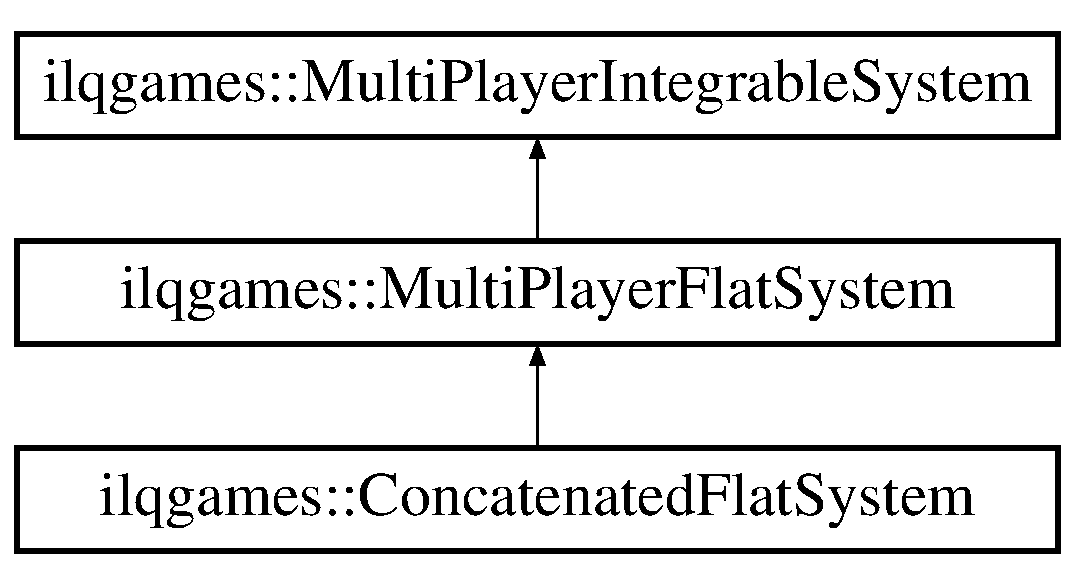
\includegraphics[height=3.000000cm]{classilqgames_1_1_multi_player_flat_system}
\end{center}
\end{figure}
\subsection*{Public Member Functions}
\begin{DoxyCompactItemize}
\item 
virtual Vector\+Xf {\bfseries Evaluate} (const Vector\+Xf \&x, const std\+::vector$<$ Vector\+Xf $>$ \&us) const =0\hypertarget{classilqgames_1_1_multi_player_flat_system_a5d05a118c1871d8d2493635fe8413652}{}\label{classilqgames_1_1_multi_player_flat_system_a5d05a118c1871d8d2493635fe8413652}

\item 
virtual Matrix\+Xf {\bfseries Inverse\+Decoupling\+Matrix} (const Vector\+Xf \&x) const =0\hypertarget{classilqgames_1_1_multi_player_flat_system_ada6148061596394fad774daa37596065}{}\label{classilqgames_1_1_multi_player_flat_system_ada6148061596394fad774daa37596065}

\item 
virtual Vector\+Xf {\bfseries Affine\+Term} (const Vector\+Xf \&x) const =0\hypertarget{classilqgames_1_1_multi_player_flat_system_a163e065f928dcf06d318c326179cfe77}{}\label{classilqgames_1_1_multi_player_flat_system_a163e065f928dcf06d318c326179cfe77}

\item 
virtual Vector\+Xf {\bfseries Linearizing\+Control} (const Vector\+Xf \&x, const Vector\+Xf \&v, Player\+Index player) const =0\hypertarget{classilqgames_1_1_multi_player_flat_system_a8208bc8f674e9336c9e02af26ab45f45}{}\label{classilqgames_1_1_multi_player_flat_system_a8208bc8f674e9336c9e02af26ab45f45}

\item 
virtual std\+::vector$<$ Vector\+Xf $>$ {\bfseries Linearizing\+Controls} (const Vector\+Xf \&x, const std\+::vector$<$ Vector\+Xf $>$ \&vs) const =0\hypertarget{classilqgames_1_1_multi_player_flat_system_adf25dd35fbef86603f2e5d0dcc733e43}{}\label{classilqgames_1_1_multi_player_flat_system_adf25dd35fbef86603f2e5d0dcc733e43}

\item 
virtual Vector\+Xf {\bfseries To\+Linear\+System\+State} (const Vector\+Xf \&x) const =0\hypertarget{classilqgames_1_1_multi_player_flat_system_a2ace258741dd490be115378fca8fb0d7}{}\label{classilqgames_1_1_multi_player_flat_system_a2ace258741dd490be115378fca8fb0d7}

\item 
virtual Vector\+Xf {\bfseries From\+Linear\+System\+State} (const Vector\+Xf \&xi) const =0\hypertarget{classilqgames_1_1_multi_player_flat_system_a0e93189c620e44698a8a873a6ce2acdc}{}\label{classilqgames_1_1_multi_player_flat_system_a0e93189c620e44698a8a873a6ce2acdc}

\item 
virtual void {\bfseries Change\+Cost\+Coordinates} (const Vector\+Xf \&xi, std\+::vector$<$ \hyperlink{structilqgames_1_1_quadratic_cost_approximation}{Quadratic\+Cost\+Approximation} $>$ $\ast$q) const =0\hypertarget{classilqgames_1_1_multi_player_flat_system_a25f774ea87c09b634ee2ab9254c847a2}{}\label{classilqgames_1_1_multi_player_flat_system_a25f774ea87c09b634ee2ab9254c847a2}

\item 
virtual void {\bfseries Change\+Control\+Cost\+Coordinates} (const Vector\+Xf \&xi, std\+::vector$<$ \hyperlink{structilqgames_1_1_quadratic_cost_approximation}{Quadratic\+Cost\+Approximation} $>$ $\ast$q) const =0\hypertarget{classilqgames_1_1_multi_player_flat_system_ac267c5a7404b415270ef296e202e9a69}{}\label{classilqgames_1_1_multi_player_flat_system_ac267c5a7404b415270ef296e202e9a69}

\item 
virtual bool {\bfseries Is\+Linear\+System\+State\+Singular} (const Vector\+Xf \&xi) const =0\hypertarget{classilqgames_1_1_multi_player_flat_system_ad6087e0a046965cafa165e0b91c522c6}{}\label{classilqgames_1_1_multi_player_flat_system_ad6087e0a046965cafa165e0b91c522c6}

\item 
Vector\+Xf {\bfseries Integrate} (Time time\+\_\+interval, const Vector\+Xf \&xi0, const std\+::vector$<$ Vector\+Xf $>$ \&vs) const \hypertarget{classilqgames_1_1_multi_player_flat_system_afb949d4a488fd42bc2e250d520ef3b1e}{}\label{classilqgames_1_1_multi_player_flat_system_afb949d4a488fd42bc2e250d520ef3b1e}

\item 
Vector\+Xf {\bfseries Integrate} (Time t0, Time time\+\_\+interval, const Vector\+Xf \&xi0, const std\+::vector$<$ Vector\+Xf $>$ \&vs) const \hypertarget{classilqgames_1_1_multi_player_flat_system_acfdf524322acc6a648bf8ace934a2786}{}\label{classilqgames_1_1_multi_player_flat_system_acfdf524322acc6a648bf8ace934a2786}

\item 
bool {\bfseries Treat\+As\+Linear} () const \hypertarget{classilqgames_1_1_multi_player_flat_system_aa84d9e22e6df454d1751eefa46db28c5}{}\label{classilqgames_1_1_multi_player_flat_system_aa84d9e22e6df454d1751eefa46db28c5}

\item 
const \hyperlink{structilqgames_1_1_linear_dynamics_approximation}{Linear\+Dynamics\+Approximation} \& {\bfseries Linearized\+System} () const \hypertarget{classilqgames_1_1_multi_player_flat_system_a7bfa1936fce9997d061c86ce37d874b6}{}\label{classilqgames_1_1_multi_player_flat_system_a7bfa1936fce9997d061c86ce37d874b6}

\item 
virtual Dimension {\bfseries U\+Dim} (Player\+Index player\+\_\+idx) const =0\hypertarget{classilqgames_1_1_multi_player_flat_system_a1cb3a0636263a35dd2b10f8b203bf29b}{}\label{classilqgames_1_1_multi_player_flat_system_a1cb3a0636263a35dd2b10f8b203bf29b}

\item 
virtual Player\+Index {\bfseries Num\+Players} () const =0\hypertarget{classilqgames_1_1_multi_player_flat_system_a5732cac3a3a64567a3d1b460d787a52d}{}\label{classilqgames_1_1_multi_player_flat_system_a5732cac3a3a64567a3d1b460d787a52d}

\end{DoxyCompactItemize}
\subsection*{Protected Member Functions}
\begin{DoxyCompactItemize}
\item 
{\bfseries Multi\+Player\+Flat\+System} (Dimension xdim, Time time\+\_\+step)\hypertarget{classilqgames_1_1_multi_player_flat_system_a73df802233de8b218744e662ab250b59}{}\label{classilqgames_1_1_multi_player_flat_system_a73df802233de8b218744e662ab250b59}

\item 
virtual void {\bfseries Compute\+Linearized\+System} () const =0\hypertarget{classilqgames_1_1_multi_player_flat_system_ab5e1b8bb3cf07f07c04d7f3884c1c015}{}\label{classilqgames_1_1_multi_player_flat_system_ab5e1b8bb3cf07f07c04d7f3884c1c015}

\end{DoxyCompactItemize}
\subsection*{Protected Attributes}
\begin{DoxyCompactItemize}
\item 
std\+::unique\+\_\+ptr$<$ const \hyperlink{structilqgames_1_1_linear_dynamics_approximation}{Linear\+Dynamics\+Approximation} $>$ {\bfseries discrete\+\_\+linear\+\_\+system\+\_\+}\hypertarget{classilqgames_1_1_multi_player_flat_system_a70c6bbb2e4cd3653594fd650fbcdad94}{}\label{classilqgames_1_1_multi_player_flat_system_a70c6bbb2e4cd3653594fd650fbcdad94}

\item 
std\+::unique\+\_\+ptr$<$ const \hyperlink{structilqgames_1_1_linear_dynamics_approximation}{Linear\+Dynamics\+Approximation} $>$ {\bfseries continuous\+\_\+linear\+\_\+system\+\_\+}\hypertarget{classilqgames_1_1_multi_player_flat_system_ab4961edf0a14f8645c79d2ad39ebd7d6}{}\label{classilqgames_1_1_multi_player_flat_system_ab4961edf0a14f8645c79d2ad39ebd7d6}

\end{DoxyCompactItemize}


\subsection{Detailed Description}


Definition at line 58 of file multi\+\_\+player\+\_\+flat\+\_\+system.\+h.



The documentation for this class was generated from the following files\+:\begin{DoxyCompactItemize}
\item 
/home/travis/build/\+H\+J\+Reachability/ilqgames/include/ilqgames/dynamics/multi\+\_\+player\+\_\+flat\+\_\+system.\+h\item 
/home/travis/build/\+H\+J\+Reachability/ilqgames/src/multi\+\_\+player\+\_\+flat\+\_\+system.\+cpp\end{DoxyCompactItemize}

\hypertarget{classilqgames_1_1_multi_player_integrable_system}{}\section{ilqgames\+:\+:Multi\+Player\+Integrable\+System Class Reference}
\label{classilqgames_1_1_multi_player_integrable_system}\index{ilqgames\+::\+Multi\+Player\+Integrable\+System@{ilqgames\+::\+Multi\+Player\+Integrable\+System}}
Inheritance diagram for ilqgames\+:\+:Multi\+Player\+Integrable\+System\+:\begin{figure}[H]
\begin{center}
\leavevmode
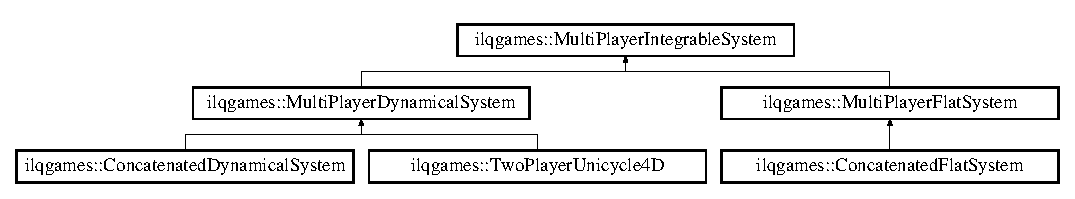
\includegraphics[height=1.673307cm]{classilqgames_1_1_multi_player_integrable_system}
\end{center}
\end{figure}
\subsection*{Public Member Functions}
\begin{DoxyCompactItemize}
\item 
virtual Vector\+Xf {\bfseries Integrate} (Time t0, Time time\+\_\+interval, const Vector\+Xf \&x0, const std\+::vector$<$ Vector\+Xf $>$ \&us) const =0\hypertarget{classilqgames_1_1_multi_player_integrable_system_a591b1d66f51b95cf6e5bd1bd3b1c6f4d}{}\label{classilqgames_1_1_multi_player_integrable_system_a591b1d66f51b95cf6e5bd1bd3b1c6f4d}

\item 
Vector\+Xf {\bfseries Integrate} (Time t0, Time t, const Vector\+Xf \&x0, const \hyperlink{structilqgames_1_1_operating_point}{Operating\+Point} \&operating\+\_\+point, const std\+::vector$<$ \hyperlink{structilqgames_1_1_strategy}{Strategy} $>$ \&strategies) const \hypertarget{classilqgames_1_1_multi_player_integrable_system_a92e9cc0b05d1402a5ccc2a45f2c16f63}{}\label{classilqgames_1_1_multi_player_integrable_system_a92e9cc0b05d1402a5ccc2a45f2c16f63}

\item 
Vector\+Xf {\bfseries Integrate} (size\+\_\+t initial\+\_\+timestep, size\+\_\+t final\+\_\+timestep, const Vector\+Xf \&x0, const \hyperlink{structilqgames_1_1_operating_point}{Operating\+Point} \&operating\+\_\+point, const std\+::vector$<$ \hyperlink{structilqgames_1_1_strategy}{Strategy} $>$ \&strategies) const \hypertarget{classilqgames_1_1_multi_player_integrable_system_a38241e3d9edb8ec9ff3c7755b755d689}{}\label{classilqgames_1_1_multi_player_integrable_system_a38241e3d9edb8ec9ff3c7755b755d689}

\item 
Vector\+Xf {\bfseries Integrate\+To\+Next\+Time\+Step} (Time t0, const Vector\+Xf \&x0, const \hyperlink{structilqgames_1_1_operating_point}{Operating\+Point} \&operating\+\_\+point, const std\+::vector$<$ \hyperlink{structilqgames_1_1_strategy}{Strategy} $>$ \&strategies) const \hypertarget{classilqgames_1_1_multi_player_integrable_system_abba5990a5ccb56588e252a05f0b84b0f}{}\label{classilqgames_1_1_multi_player_integrable_system_abba5990a5ccb56588e252a05f0b84b0f}

\item 
Vector\+Xf {\bfseries Integrate\+From\+Prior\+Time\+Step} (Time t, const Vector\+Xf \&x0, const \hyperlink{structilqgames_1_1_operating_point}{Operating\+Point} \&operating\+\_\+point, const std\+::vector$<$ \hyperlink{structilqgames_1_1_strategy}{Strategy} $>$ \&strategies) const \hypertarget{classilqgames_1_1_multi_player_integrable_system_ada6af6c39bac2fda2043302b0e6c965c}{}\label{classilqgames_1_1_multi_player_integrable_system_ada6af6c39bac2fda2043302b0e6c965c}

\item 
Vector\+Xf {\bfseries Integrate} (Time t0, Time time\+\_\+interval, const Eigen\+::\+Ref$<$ Vector\+Xf $>$ \&x0, const std\+::vector$<$ Eigen\+::\+Ref$<$ Vector\+Xf $>$$>$ \&us) const \hypertarget{classilqgames_1_1_multi_player_integrable_system_afa891d5a1184cefdc316f76528d01a0e}{}\label{classilqgames_1_1_multi_player_integrable_system_afa891d5a1184cefdc316f76528d01a0e}

\item 
virtual bool {\bfseries Treat\+As\+Linear} () const \hypertarget{classilqgames_1_1_multi_player_integrable_system_adf8ab89fd04892a1806814ef4ce89188}{}\label{classilqgames_1_1_multi_player_integrable_system_adf8ab89fd04892a1806814ef4ce89188}

\item 
virtual Vector\+Xf {\bfseries Stitch} (const Vector\+Xf \&x\+\_\+ego, const Vector\+Xf \&x\+\_\+others) const \hypertarget{classilqgames_1_1_multi_player_integrable_system_a027ab5dea23c68ea74040a50a7b16c31}{}\label{classilqgames_1_1_multi_player_integrable_system_a027ab5dea23c68ea74040a50a7b16c31}

\item 
Dimension {\bfseries X\+Dim} () const \hypertarget{classilqgames_1_1_multi_player_integrable_system_a1f3d72304e04f6906e6e1066717411a7}{}\label{classilqgames_1_1_multi_player_integrable_system_a1f3d72304e04f6906e6e1066717411a7}

\item 
Dimension {\bfseries Total\+U\+Dim} () const \hypertarget{classilqgames_1_1_multi_player_integrable_system_ac6fc71106bffdff776a55792af4560d1}{}\label{classilqgames_1_1_multi_player_integrable_system_ac6fc71106bffdff776a55792af4560d1}

\item 
virtual Dimension {\bfseries U\+Dim} (Player\+Index player\+\_\+idx) const =0\hypertarget{classilqgames_1_1_multi_player_integrable_system_a89563d59d8cda88e0825992b86c9a146}{}\label{classilqgames_1_1_multi_player_integrable_system_a89563d59d8cda88e0825992b86c9a146}

\item 
virtual Player\+Index {\bfseries Num\+Players} () const =0\hypertarget{classilqgames_1_1_multi_player_integrable_system_a894daac1bf9f941718529e5a31b81a88}{}\label{classilqgames_1_1_multi_player_integrable_system_a894daac1bf9f941718529e5a31b81a88}

\item 
virtual std\+::vector$<$ Dimension $>$ {\bfseries Position\+Dimensions} () const =0\hypertarget{classilqgames_1_1_multi_player_integrable_system_aa997a26ebcf8aaa4ec80b22fa996d574}{}\label{classilqgames_1_1_multi_player_integrable_system_aa997a26ebcf8aaa4ec80b22fa996d574}

\item 
virtual float {\bfseries Distance\+Between} (const Vector\+Xf \&x0, const Vector\+Xf \&x1) const \hypertarget{classilqgames_1_1_multi_player_integrable_system_af25dee45970bc4e53a3844084bc3fad4}{}\label{classilqgames_1_1_multi_player_integrable_system_af25dee45970bc4e53a3844084bc3fad4}

\end{DoxyCompactItemize}
\subsection*{Static Public Member Functions}
\begin{DoxyCompactItemize}
\item 
static void {\bfseries Integrate\+Using\+Euler} ()\hypertarget{classilqgames_1_1_multi_player_integrable_system_afbe59f8e51163913a0ef03b84bf6b33b}{}\label{classilqgames_1_1_multi_player_integrable_system_afbe59f8e51163913a0ef03b84bf6b33b}

\item 
static void {\bfseries Integrate\+Using\+R\+K4} ()\hypertarget{classilqgames_1_1_multi_player_integrable_system_a8623ddb41f2ea72b1838d5f8292fe091}{}\label{classilqgames_1_1_multi_player_integrable_system_a8623ddb41f2ea72b1838d5f8292fe091}

\item 
static bool {\bfseries Integration\+Uses\+Euler} ()\hypertarget{classilqgames_1_1_multi_player_integrable_system_a7d8d977e079520ad4eb6e2e38833b25c}{}\label{classilqgames_1_1_multi_player_integrable_system_a7d8d977e079520ad4eb6e2e38833b25c}

\end{DoxyCompactItemize}
\subsection*{Protected Member Functions}
\begin{DoxyCompactItemize}
\item 
{\bfseries Multi\+Player\+Integrable\+System} (Dimension xdim)\hypertarget{classilqgames_1_1_multi_player_integrable_system_a0c950b1732a06fe9b98392b3b83109f6}{}\label{classilqgames_1_1_multi_player_integrable_system_a0c950b1732a06fe9b98392b3b83109f6}

\end{DoxyCompactItemize}
\subsection*{Protected Attributes}
\begin{DoxyCompactItemize}
\item 
const Dimension {\bfseries xdim\+\_\+}\hypertarget{classilqgames_1_1_multi_player_integrable_system_ad6f5958f0f51492aa1d368765f417a19}{}\label{classilqgames_1_1_multi_player_integrable_system_ad6f5958f0f51492aa1d368765f417a19}

\end{DoxyCompactItemize}
\subsection*{Static Protected Attributes}
\begin{DoxyCompactItemize}
\item 
static bool {\bfseries integrate\+\_\+using\+\_\+euler\+\_\+} = false\hypertarget{classilqgames_1_1_multi_player_integrable_system_a45d12b2d86a80f04fac29bd88eb8179a}{}\label{classilqgames_1_1_multi_player_integrable_system_a45d12b2d86a80f04fac29bd88eb8179a}

\end{DoxyCompactItemize}


\subsection{Detailed Description}


Definition at line 55 of file multi\+\_\+player\+\_\+integrable\+\_\+system.\+h.



The documentation for this class was generated from the following files\+:\begin{DoxyCompactItemize}
\item 
/home/travis/build/\+H\+J\+Reachability/ilqgames/include/ilqgames/dynamics/multi\+\_\+player\+\_\+integrable\+\_\+system.\+h\item 
/home/travis/build/\+H\+J\+Reachability/ilqgames/src/multi\+\_\+player\+\_\+integrable\+\_\+system.\+cpp\end{DoxyCompactItemize}

\hypertarget{classilqgames_1_1_nominal_path_length_cost}{}\section{ilqgames\+:\+:Nominal\+Path\+Length\+Cost Class Reference}
\label{classilqgames_1_1_nominal_path_length_cost}\index{ilqgames\+::\+Nominal\+Path\+Length\+Cost@{ilqgames\+::\+Nominal\+Path\+Length\+Cost}}
Inheritance diagram for ilqgames\+:\+:Nominal\+Path\+Length\+Cost\+:\begin{figure}[H]
\begin{center}
\leavevmode
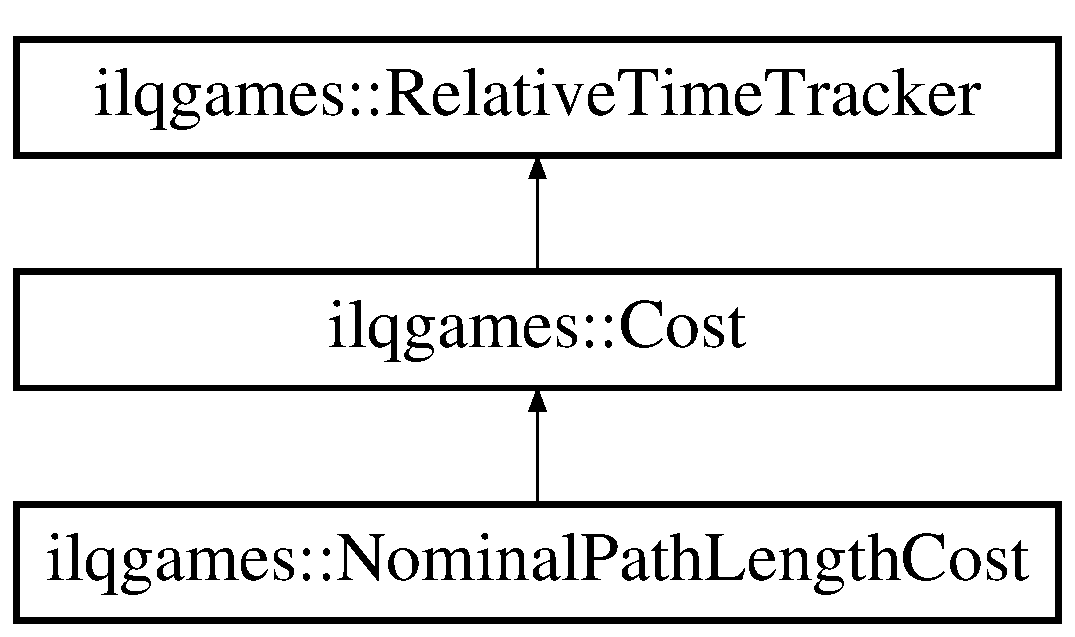
\includegraphics[height=3.000000cm]{classilqgames_1_1_nominal_path_length_cost}
\end{center}
\end{figure}
\subsection*{Public Member Functions}
\begin{DoxyCompactItemize}
\item 
{\bfseries Nominal\+Path\+Length\+Cost} (float weight, Dimension dim, float nominal\+\_\+speed, const std\+::string \&name=\char`\"{}\char`\"{})\hypertarget{classilqgames_1_1_nominal_path_length_cost_a2dbd457c7e1b6c202d7c5f3b72bcecde}{}\label{classilqgames_1_1_nominal_path_length_cost_a2dbd457c7e1b6c202d7c5f3b72bcecde}

\item 
float {\bfseries Evaluate} (Time t, const Vector\+Xf \&input) const \hypertarget{classilqgames_1_1_nominal_path_length_cost_a3a8ac79f9c35f39328a0a7829881386f}{}\label{classilqgames_1_1_nominal_path_length_cost_a3a8ac79f9c35f39328a0a7829881386f}

\item 
void {\bfseries Quadraticize} (Time t, const Vector\+Xf \&input, Matrix\+Xf $\ast$hess, Vector\+Xf $\ast$grad) const \hypertarget{classilqgames_1_1_nominal_path_length_cost_a91f8dbf5342e12dea4ff405ac65a3184}{}\label{classilqgames_1_1_nominal_path_length_cost_a91f8dbf5342e12dea4ff405ac65a3184}

\end{DoxyCompactItemize}
\subsection*{Additional Inherited Members}


\subsection{Detailed Description}


Definition at line 54 of file nominal\+\_\+path\+\_\+length\+\_\+cost.\+h.



The documentation for this class was generated from the following files\+:\begin{DoxyCompactItemize}
\item 
/home/travis/build/\+H\+J\+Reachability/ilqgames/include/ilqgames/cost/nominal\+\_\+path\+\_\+length\+\_\+cost.\+h\item 
/home/travis/build/\+H\+J\+Reachability/ilqgames/src/nominal\+\_\+path\+\_\+length\+\_\+cost.\+cpp\end{DoxyCompactItemize}

\hypertarget{classilqgames_1_1_one_player_reachability_example}{}\section{ilqgames\+:\+:One\+Player\+Reachability\+Example Class Reference}
\label{classilqgames_1_1_one_player_reachability_example}\index{ilqgames\+::\+One\+Player\+Reachability\+Example@{ilqgames\+::\+One\+Player\+Reachability\+Example}}
Inheritance diagram for ilqgames\+:\+:One\+Player\+Reachability\+Example\+:\begin{figure}[H]
\begin{center}
\leavevmode
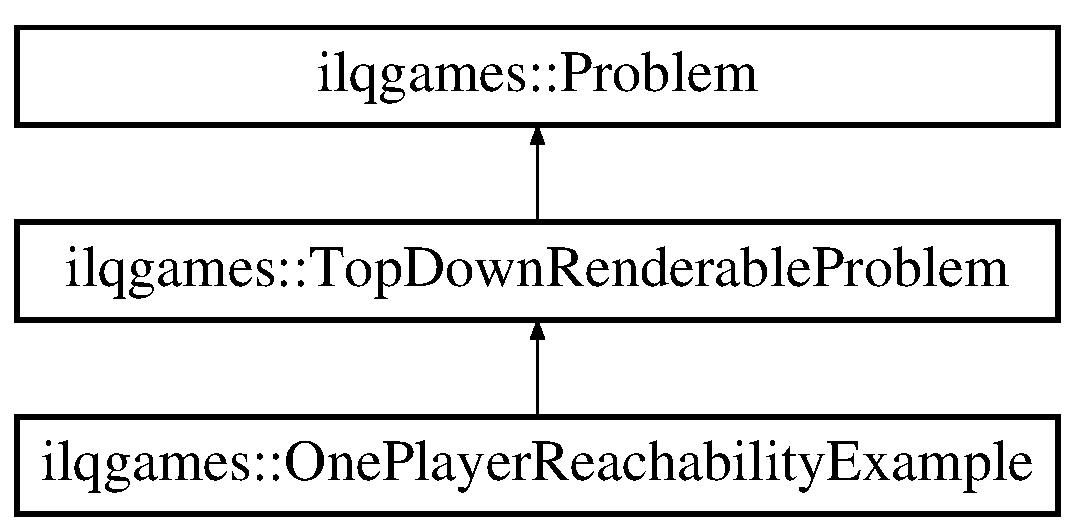
\includegraphics[height=3.000000cm]{classilqgames_1_1_one_player_reachability_example}
\end{center}
\end{figure}
\subsection*{Public Member Functions}
\begin{DoxyCompactItemize}
\item 
void {\bfseries Construct\+Dynamics} ()\hypertarget{classilqgames_1_1_one_player_reachability_example_a48964bc13dc22a0fb6c264ae8733fe56}{}\label{classilqgames_1_1_one_player_reachability_example_a48964bc13dc22a0fb6c264ae8733fe56}

\item 
void {\bfseries Construct\+Initial\+State} ()\hypertarget{classilqgames_1_1_one_player_reachability_example_adfd432f2c753649e32c91b74aacf227e}{}\label{classilqgames_1_1_one_player_reachability_example_adfd432f2c753649e32c91b74aacf227e}

\item 
void {\bfseries Construct\+Player\+Costs} ()\hypertarget{classilqgames_1_1_one_player_reachability_example_adea4adbb46e7797d26aa86f0039577e9}{}\label{classilqgames_1_1_one_player_reachability_example_adea4adbb46e7797d26aa86f0039577e9}

\item 
std\+::vector$<$ float $>$ {\bfseries Xs} (const Vector\+Xf \&x) const \hypertarget{classilqgames_1_1_one_player_reachability_example_a1209e4293042afbb8aa9b4cd6f8af7c6}{}\label{classilqgames_1_1_one_player_reachability_example_a1209e4293042afbb8aa9b4cd6f8af7c6}

\item 
std\+::vector$<$ float $>$ {\bfseries Ys} (const Vector\+Xf \&x) const \hypertarget{classilqgames_1_1_one_player_reachability_example_affa80730ce318688c06f7b54163bf80f}{}\label{classilqgames_1_1_one_player_reachability_example_affa80730ce318688c06f7b54163bf80f}

\item 
std\+::vector$<$ float $>$ {\bfseries Thetas} (const Vector\+Xf \&x) const \hypertarget{classilqgames_1_1_one_player_reachability_example_ad4a4dffe34cfff22eae36e5c3235c3ff}{}\label{classilqgames_1_1_one_player_reachability_example_ad4a4dffe34cfff22eae36e5c3235c3ff}

\end{DoxyCompactItemize}
\subsection*{Additional Inherited Members}


\subsection{Detailed Description}


Definition at line 52 of file one\+\_\+player\+\_\+reachability\+\_\+example.\+h.



The documentation for this class was generated from the following files\+:\begin{DoxyCompactItemize}
\item 
/home/travis/build/\+H\+J\+Reachability/ilqgames/include/ilqgames/examples/one\+\_\+player\+\_\+reachability\+\_\+example.\+h\item 
/home/travis/build/\+H\+J\+Reachability/ilqgames/src/one\+\_\+player\+\_\+reachability\+\_\+example.\+cpp\end{DoxyCompactItemize}

\hypertarget{structilqgames_1_1_operating_point}{}\section{ilqgames\+:\+:Operating\+Point Struct Reference}
\label{structilqgames_1_1_operating_point}\index{ilqgames\+::\+Operating\+Point@{ilqgames\+::\+Operating\+Point}}
\subsection*{Public Member Functions}
\begin{DoxyCompactItemize}
\item 
{\bfseries Operating\+Point} (size\+\_\+t num\+\_\+time\+\_\+steps, Player\+Index num\+\_\+players, Time initial\+\_\+time)\hypertarget{structilqgames_1_1_operating_point_a28dab0579fa6ece2f983c8eec32d6819}{}\label{structilqgames_1_1_operating_point_a28dab0579fa6ece2f983c8eec32d6819}

\item 
{\footnotesize template$<$typename Multi\+Player\+System\+Type $>$ }\\{\bfseries Operating\+Point} (size\+\_\+t num\+\_\+time\+\_\+steps, Player\+Index num\+\_\+players, Time initial\+\_\+time, const std\+::shared\+\_\+ptr$<$ const Multi\+Player\+System\+Type $>$ \&dynamics)\hypertarget{structilqgames_1_1_operating_point_aa7027d31067aa2a098a57b123eda53f8}{}\label{structilqgames_1_1_operating_point_aa7027d31067aa2a098a57b123eda53f8}

\item 
void {\bfseries swap} (\hyperlink{structilqgames_1_1_operating_point}{Operating\+Point} \&other)\hypertarget{structilqgames_1_1_operating_point_a373b480b0f424863bb2dfaced7cd2f6f}{}\label{structilqgames_1_1_operating_point_a373b480b0f424863bb2dfaced7cd2f6f}

\end{DoxyCompactItemize}
\subsection*{Public Attributes}
\begin{DoxyCompactItemize}
\item 
std\+::vector$<$ Vector\+Xf $>$ {\bfseries xs}\hypertarget{structilqgames_1_1_operating_point_a8d92a8f89457d4498cf0084e6752570d}{}\label{structilqgames_1_1_operating_point_a8d92a8f89457d4498cf0084e6752570d}

\item 
std\+::vector$<$ std\+::vector$<$ Vector\+Xf $>$ $>$ {\bfseries us}\hypertarget{structilqgames_1_1_operating_point_a69c62d532a1ab13a70e5dc40aede8a6a}{}\label{structilqgames_1_1_operating_point_a69c62d532a1ab13a70e5dc40aede8a6a}

\item 
Time {\bfseries t0}\hypertarget{structilqgames_1_1_operating_point_a04e5e484159428a29d8aa71cb83e5542}{}\label{structilqgames_1_1_operating_point_a04e5e484159428a29d8aa71cb83e5542}

\end{DoxyCompactItemize}


\subsection{Detailed Description}


Definition at line 55 of file operating\+\_\+point.\+h.



The documentation for this struct was generated from the following files\+:\begin{DoxyCompactItemize}
\item 
/home/travis/build/\+H\+J\+Reachability/ilqgames/include/ilqgames/utils/operating\+\_\+point.\+h\item 
/home/travis/build/\+H\+J\+Reachability/ilqgames/src/operating\+\_\+point.\+cpp\end{DoxyCompactItemize}

\hypertarget{classilqgames_1_1_orientation_cost}{}\section{ilqgames\+:\+:Orientation\+Cost Class Reference}
\label{classilqgames_1_1_orientation_cost}\index{ilqgames\+::\+Orientation\+Cost@{ilqgames\+::\+Orientation\+Cost}}
Inheritance diagram for ilqgames\+:\+:Orientation\+Cost\+:\begin{figure}[H]
\begin{center}
\leavevmode
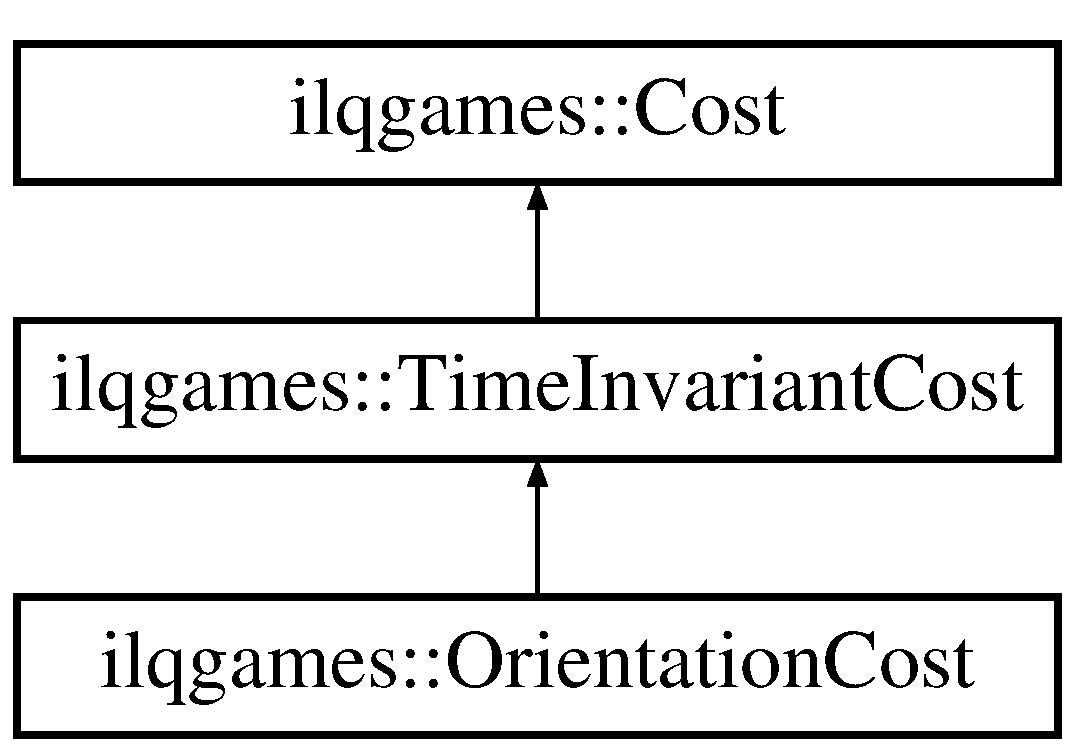
\includegraphics[height=3.000000cm]{classilqgames_1_1_orientation_cost}
\end{center}
\end{figure}
\subsection*{Public Member Functions}
\begin{DoxyCompactItemize}
\item 
{\bfseries Orientation\+Cost} (float weight, Dimension dim, float nominal=0.\+0, const std\+::string \&name=\char`\"{}\char`\"{})\hypertarget{classilqgames_1_1_orientation_cost_a9a63ce77337909590ea8fcfe164145f7}{}\label{classilqgames_1_1_orientation_cost_a9a63ce77337909590ea8fcfe164145f7}

\item 
float {\bfseries Evaluate} (const Vector\+Xf \&input) const \hypertarget{classilqgames_1_1_orientation_cost_a8003d9ccc4642698d6782901396b68d8}{}\label{classilqgames_1_1_orientation_cost_a8003d9ccc4642698d6782901396b68d8}

\item 
void {\bfseries Quadraticize} (const Vector\+Xf \&input, Matrix\+Xf $\ast$hess, Vector\+Xf $\ast$grad) const \hypertarget{classilqgames_1_1_orientation_cost_a1865ba5ee634d5dcfa52e937dcda21fd}{}\label{classilqgames_1_1_orientation_cost_a1865ba5ee634d5dcfa52e937dcda21fd}

\end{DoxyCompactItemize}
\subsection*{Additional Inherited Members}


\subsection{Detailed Description}


Definition at line 55 of file orientation\+\_\+cost.\+h.



The documentation for this class was generated from the following files\+:\begin{DoxyCompactItemize}
\item 
/home/travis/build/\+H\+J\+Reachability/ilqgames/include/ilqgames/cost/orientation\+\_\+cost.\+h\item 
/home/travis/build/\+H\+J\+Reachability/ilqgames/src/orientation\+\_\+cost.\+cpp\end{DoxyCompactItemize}

\hypertarget{classilqgames_1_1_player_cost}{}\section{ilqgames\+:\+:Player\+Cost Class Reference}
\label{classilqgames_1_1_player_cost}\index{ilqgames\+::\+Player\+Cost@{ilqgames\+::\+Player\+Cost}}
\subsection*{Public Member Functions}
\begin{DoxyCompactItemize}
\item 
{\bfseries Player\+Cost} (float state\+\_\+regularization=0.\+0, float control\+\_\+regularization=0.\+0)\hypertarget{classilqgames_1_1_player_cost_a983c96844cf283233a3c041b58453349}{}\label{classilqgames_1_1_player_cost_a983c96844cf283233a3c041b58453349}

\item 
void {\bfseries Add\+State\+Cost} (const std\+::shared\+\_\+ptr$<$ \hyperlink{classilqgames_1_1_cost}{Cost} $>$ \&cost)\hypertarget{classilqgames_1_1_player_cost_a3135d5f4c7722edc1ae385e0ecafcc87}{}\label{classilqgames_1_1_player_cost_a3135d5f4c7722edc1ae385e0ecafcc87}

\item 
void {\bfseries Add\+Control\+Cost} (Player\+Index idx, const std\+::shared\+\_\+ptr$<$ \hyperlink{classilqgames_1_1_cost}{Cost} $>$ \&cost)\hypertarget{classilqgames_1_1_player_cost_aba4df0e6414aba024c86bf77fe57f819}{}\label{classilqgames_1_1_player_cost_aba4df0e6414aba024c86bf77fe57f819}

\item 
void {\bfseries Add\+State\+Constraint} (const std\+::shared\+\_\+ptr$<$ \hyperlink{classilqgames_1_1_constraint}{Constraint} $>$ \&constraint)\hypertarget{classilqgames_1_1_player_cost_a9c1a21f669ab3f937c3be8a49bf7b5b3}{}\label{classilqgames_1_1_player_cost_a9c1a21f669ab3f937c3be8a49bf7b5b3}

\item 
void {\bfseries Add\+Control\+Constraint} (Player\+Index idx, const std\+::shared\+\_\+ptr$<$ \hyperlink{classilqgames_1_1_constraint}{Constraint} $>$ \&constraint)\hypertarget{classilqgames_1_1_player_cost_a9df6549112ab9b03bd639b4955b700da}{}\label{classilqgames_1_1_player_cost_a9df6549112ab9b03bd639b4955b700da}

\item 
float {\bfseries Evaluate} (Time t, const Vector\+Xf \&x, const std\+::vector$<$ Vector\+Xf $>$ \&us) const \hypertarget{classilqgames_1_1_player_cost_ac1ad99a1822d97a53d084fd9da162cb1}{}\label{classilqgames_1_1_player_cost_ac1ad99a1822d97a53d084fd9da162cb1}

\item 
float {\bfseries Evaluate} (const \hyperlink{structilqgames_1_1_operating_point}{Operating\+Point} \&op, Time time\+\_\+step) const \hypertarget{classilqgames_1_1_player_cost_a8c7fc17986dfb478df17cf9f8da85926}{}\label{classilqgames_1_1_player_cost_a8c7fc17986dfb478df17cf9f8da85926}

\item 
float {\bfseries Evaluate\+Offset} (Time t, Time next\+\_\+t, const Vector\+Xf \&next\+\_\+x, const std\+::vector$<$ Vector\+Xf $>$ \&us) const \hypertarget{classilqgames_1_1_player_cost_a56bf9c10b7ffa6fbdfb1a9bff1ce65c3}{}\label{classilqgames_1_1_player_cost_a56bf9c10b7ffa6fbdfb1a9bff1ce65c3}

\item 
\hyperlink{structilqgames_1_1_quadratic_cost_approximation}{Quadratic\+Cost\+Approximation} {\bfseries Quadraticize} (Time t, const Vector\+Xf \&x, const std\+::vector$<$ Vector\+Xf $>$ \&us) const \hypertarget{classilqgames_1_1_player_cost_ad3962847f8eda8bcfecf2096e6abccb6}{}\label{classilqgames_1_1_player_cost_ad3962847f8eda8bcfecf2096e6abccb6}

\item 
bool {\bfseries Check\+Constraints} (Time t, const Vector\+Xf \&x) const \hypertarget{classilqgames_1_1_player_cost_aecd3478584357f4ea5d743c14b842e71}{}\label{classilqgames_1_1_player_cost_aecd3478584357f4ea5d743c14b842e71}

\item 
void {\bfseries Scale\+Constraint\+Barrier\+Weights} (float scale=0.\+5)\hypertarget{classilqgames_1_1_player_cost_a01099622def541cf226c94140c38d485}{}\label{classilqgames_1_1_player_cost_a01099622def541cf226c94140c38d485}

\item 
void {\bfseries Reset\+Constraint\+Barrier\+Weights} ()\hypertarget{classilqgames_1_1_player_cost_add7445e01947fcaaf9d5f1e392471970}{}\label{classilqgames_1_1_player_cost_add7445e01947fcaaf9d5f1e392471970}

\item 
const std\+::vector$<$ std\+::shared\+\_\+ptr$<$ \hyperlink{classilqgames_1_1_cost}{Cost} $>$ $>$ \& {\bfseries State\+Costs} () const \hypertarget{classilqgames_1_1_player_cost_adfb1861f05ba2efa163e7a28670f0585}{}\label{classilqgames_1_1_player_cost_adfb1861f05ba2efa163e7a28670f0585}

\item 
const Cost\+Map$<$ \hyperlink{classilqgames_1_1_cost}{Cost} $>$ \& {\bfseries Control\+Costs} () const \hypertarget{classilqgames_1_1_player_cost_a4fa0717c227acf2773deda56eaf62e99}{}\label{classilqgames_1_1_player_cost_a4fa0717c227acf2773deda56eaf62e99}

\item 
const std\+::vector$<$ std\+::shared\+\_\+ptr$<$ \hyperlink{classilqgames_1_1_constraint}{Constraint} $>$ $>$ \& {\bfseries State\+Constraints} () const \hypertarget{classilqgames_1_1_player_cost_ac6ef894e71fd9524bd6aa6d3982f415a}{}\label{classilqgames_1_1_player_cost_ac6ef894e71fd9524bd6aa6d3982f415a}

\item 
const Cost\+Map$<$ \hyperlink{classilqgames_1_1_constraint}{Constraint} $>$ \& {\bfseries Control\+Constraints} () const \hypertarget{classilqgames_1_1_player_cost_acf0081bb561f71522cd9716a9e34eb60}{}\label{classilqgames_1_1_player_cost_acf0081bb561f71522cd9716a9e34eb60}

\end{DoxyCompactItemize}


\subsection{Detailed Description}


Definition at line 57 of file player\+\_\+cost.\+h.



The documentation for this class was generated from the following files\+:\begin{DoxyCompactItemize}
\item 
/home/travis/build/\+H\+J\+Reachability/ilqgames/include/ilqgames/cost/player\+\_\+cost.\+h\item 
/home/travis/build/\+H\+J\+Reachability/ilqgames/src/player\+\_\+cost.\+cpp\end{DoxyCompactItemize}

\hypertarget{classilqgames_1_1_player_cost_cache}{}\section{ilqgames\+:\+:Player\+Cost\+Cache Class Reference}
\label{classilqgames_1_1_player_cost_cache}\index{ilqgames\+::\+Player\+Cost\+Cache@{ilqgames\+::\+Player\+Cost\+Cache}}
\subsection*{Public Member Functions}
\begin{DoxyCompactItemize}
\item 
{\bfseries Player\+Cost\+Cache} (const std\+::shared\+\_\+ptr$<$ const \hyperlink{classilqgames_1_1_solver_log}{Solver\+Log} $>$ \&log, const std\+::vector$<$ \hyperlink{classilqgames_1_1_player_cost}{Player\+Cost} $>$ \&player\+\_\+costs)\hypertarget{classilqgames_1_1_player_cost_cache_adbd5ce8295698ea99050b13dbc6055e5}{}\label{classilqgames_1_1_player_cost_cache_adbd5ce8295698ea99050b13dbc6055e5}

\item 
float {\bfseries Interpolate} (size\+\_\+t iterate, Time t, Player\+Index player, const std\+::string \&name) const \hypertarget{classilqgames_1_1_player_cost_cache_a9eb65722d7e25bb7f6363219122c4333}{}\label{classilqgames_1_1_player_cost_cache_a9eb65722d7e25bb7f6363219122c4333}

\item 
const \hyperlink{classilqgames_1_1_solver_log}{Solver\+Log} \& {\bfseries Log} () const \hypertarget{classilqgames_1_1_player_cost_cache_a3817f43d253d3121696c147dd37ae20f}{}\label{classilqgames_1_1_player_cost_cache_a3817f43d253d3121696c147dd37ae20f}

\item 
size\+\_\+t {\bfseries Num\+Players} () const \hypertarget{classilqgames_1_1_player_cost_cache_ad210288d53af5528c322ab60bbb4cb82}{}\label{classilqgames_1_1_player_cost_cache_ad210288d53af5528c322ab60bbb4cb82}

\item 
size\+\_\+t {\bfseries Num\+Costs} (Player\+Index player) const \hypertarget{classilqgames_1_1_player_cost_cache_af8d8c5a7804f28f7d0265f7e0f432762}{}\label{classilqgames_1_1_player_cost_cache_af8d8c5a7804f28f7d0265f7e0f432762}

\item 
bool {\bfseries Player\+Has\+Cost} (Player\+Index player, const std\+::string \&name) const \hypertarget{classilqgames_1_1_player_cost_cache_a01b366ade3f588b5d5bc743a45f9e603}{}\label{classilqgames_1_1_player_cost_cache_a01b366ade3f588b5d5bc743a45f9e603}

\item 
const std\+::unordered\+\_\+map$<$ std\+::string, std\+::vector$<$ std\+::vector$<$ float $>$ $>$ $>$ \& {\bfseries Evaluated\+Costs} (Player\+Index player) const \hypertarget{classilqgames_1_1_player_cost_cache_a73ac0a7ad44ca59451ebafce96af788a}{}\label{classilqgames_1_1_player_cost_cache_a73ac0a7ad44ca59451ebafce96af788a}

\item 
const std\+::vector$<$ float $>$ \& {\bfseries Evaluated\+Cost} (size\+\_\+t iterate, Player\+Index player, const std\+::string \&name) const \hypertarget{classilqgames_1_1_player_cost_cache_a95f82d286ddb9c91a31ad88fd13eeabc}{}\label{classilqgames_1_1_player_cost_cache_a95f82d286ddb9c91a31ad88fd13eeabc}

\end{DoxyCompactItemize}


\subsection{Detailed Description}


Definition at line 59 of file player\+\_\+cost\+\_\+cache.\+h.



The documentation for this class was generated from the following files\+:\begin{DoxyCompactItemize}
\item 
/home/travis/build/\+H\+J\+Reachability/ilqgames/include/ilqgames/utils/player\+\_\+cost\+\_\+cache.\+h\item 
/home/travis/build/\+H\+J\+Reachability/ilqgames/src/player\+\_\+cost\+\_\+cache.\+cpp\end{DoxyCompactItemize}

\hypertarget{classilqgames_1_1_polyline2}{}\section{ilqgames\+:\+:Polyline2 Class Reference}
\label{classilqgames_1_1_polyline2}\index{ilqgames\+::\+Polyline2@{ilqgames\+::\+Polyline2}}
\subsection*{Public Member Functions}
\begin{DoxyCompactItemize}
\item 
{\bfseries Polyline2} (const Point\+List2 \&points)\hypertarget{classilqgames_1_1_polyline2_a7ea13438c7c3a9b9501311684d797055}{}\label{classilqgames_1_1_polyline2_a7ea13438c7c3a9b9501311684d797055}

\item 
void {\bfseries Add\+Point} (const Point2 \&point)\hypertarget{classilqgames_1_1_polyline2_af8accf55b36d8aaa7c1ba77f4223b7f4}{}\label{classilqgames_1_1_polyline2_af8accf55b36d8aaa7c1ba77f4223b7f4}

\item 
float {\bfseries Length} () const \hypertarget{classilqgames_1_1_polyline2_ad775da2cbcd5c0c2bcc56109b6b4925e}{}\label{classilqgames_1_1_polyline2_ad775da2cbcd5c0c2bcc56109b6b4925e}

\item 
Point2 {\bfseries Closest\+Point} (const Point2 \&query, bool $\ast$is\+\_\+vertex=nullptr, \hyperlink{classilqgames_1_1_line_segment2}{Line\+Segment2} $\ast$segment=nullptr, float $\ast$signed\+\_\+squared\+\_\+distance=nullptr, bool $\ast$is\+\_\+endpoint=nullptr) const \hypertarget{classilqgames_1_1_polyline2_adbd12b8e9e9649b5ad81a84cc7069185}{}\label{classilqgames_1_1_polyline2_adbd12b8e9e9649b5ad81a84cc7069185}

\item 
Point2 {\bfseries Point\+At} (float route\+\_\+pos, bool $\ast$is\+\_\+vertex=nullptr, \hyperlink{classilqgames_1_1_line_segment2}{Line\+Segment2} $\ast$segment=nullptr, bool $\ast$is\+\_\+endpoint=nullptr) const \hypertarget{classilqgames_1_1_polyline2_a6446ad1ee2da0167046af97f620ffe57}{}\label{classilqgames_1_1_polyline2_a6446ad1ee2da0167046af97f620ffe57}

\item 
const std\+::vector$<$ \hyperlink{classilqgames_1_1_line_segment2}{Line\+Segment2} $>$ \& {\bfseries Segments} () const \hypertarget{classilqgames_1_1_polyline2_a7b840910feca7a921e29b919bb884e42}{}\label{classilqgames_1_1_polyline2_a7b840910feca7a921e29b919bb884e42}

\end{DoxyCompactItemize}


\subsection{Detailed Description}


Definition at line 54 of file polyline2.\+h.



The documentation for this class was generated from the following files\+:\begin{DoxyCompactItemize}
\item 
/home/travis/build/\+H\+J\+Reachability/ilqgames/include/ilqgames/geometry/polyline2.\+h\item 
/home/travis/build/\+H\+J\+Reachability/ilqgames/src/polyline2.\+cpp\end{DoxyCompactItemize}

\hypertarget{classilqgames_1_1_polyline2_signed_distance_constraint}{}\section{ilqgames\+:\+:Polyline2\+Signed\+Distance\+Constraint Class Reference}
\label{classilqgames_1_1_polyline2_signed_distance_constraint}\index{ilqgames\+::\+Polyline2\+Signed\+Distance\+Constraint@{ilqgames\+::\+Polyline2\+Signed\+Distance\+Constraint}}
Inheritance diagram for ilqgames\+:\+:Polyline2\+Signed\+Distance\+Constraint\+:\begin{figure}[H]
\begin{center}
\leavevmode
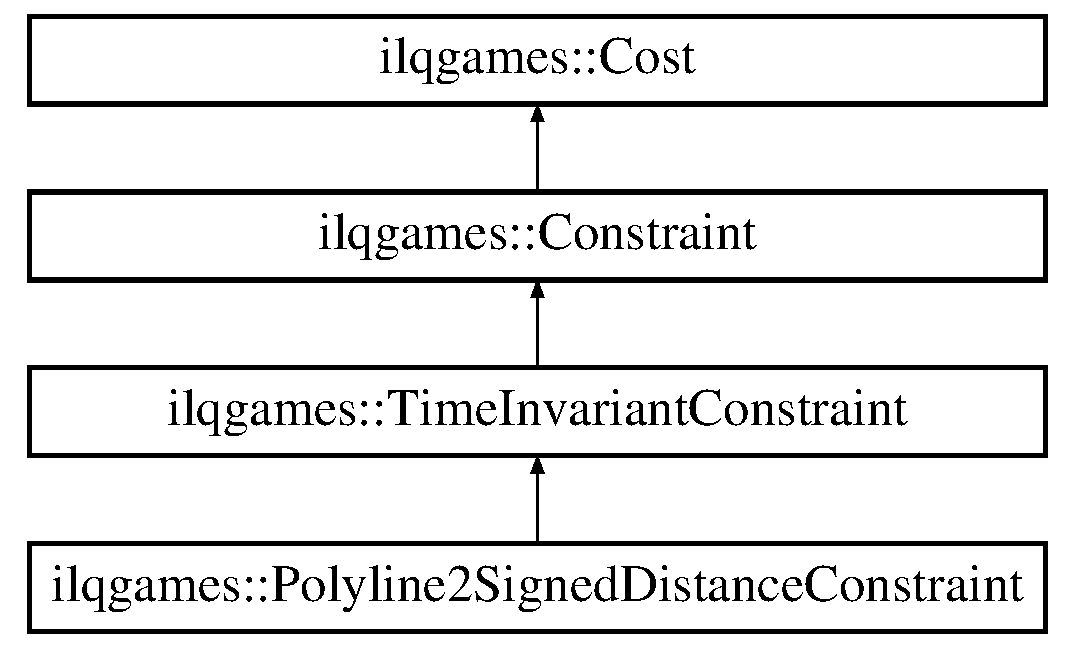
\includegraphics[height=4.000000cm]{classilqgames_1_1_polyline2_signed_distance_constraint}
\end{center}
\end{figure}
\subsection*{Public Member Functions}
\begin{DoxyCompactItemize}
\item 
{\bfseries Polyline2\+Signed\+Distance\+Constraint} (const \hyperlink{classilqgames_1_1_polyline2}{Polyline2} \&polyline, const std\+::pair$<$ Dimension, Dimension $>$ \&position\+\_\+idxs, float threshold, bool oriented\+\_\+right, const std\+::string \&name=\char`\"{}\char`\"{})\hypertarget{classilqgames_1_1_polyline2_signed_distance_constraint_acbcaeeb0b52b5de6fc25a03487677bc1}{}\label{classilqgames_1_1_polyline2_signed_distance_constraint_acbcaeeb0b52b5de6fc25a03487677bc1}

\item 
bool {\bfseries Is\+Satisfied\+Level} (const Vector\+Xf \&input, float $\ast$level) const \hypertarget{classilqgames_1_1_polyline2_signed_distance_constraint_ac30e6fad83247ddc86f3cb69a6e4d8cc}{}\label{classilqgames_1_1_polyline2_signed_distance_constraint_ac30e6fad83247ddc86f3cb69a6e4d8cc}

\item 
void {\bfseries Quadraticize} (const Vector\+Xf \&input, Matrix\+Xf $\ast$hess, Vector\+Xf $\ast$grad) const \hypertarget{classilqgames_1_1_polyline2_signed_distance_constraint_a0468a14f66cc448cc21a1351c393ec21}{}\label{classilqgames_1_1_polyline2_signed_distance_constraint_a0468a14f66cc448cc21a1351c393ec21}

\end{DoxyCompactItemize}
\subsection*{Additional Inherited Members}


\subsection{Detailed Description}


Definition at line 58 of file polyline2\+\_\+signed\+\_\+distance\+\_\+constraint.\+h.



The documentation for this class was generated from the following files\+:\begin{DoxyCompactItemize}
\item 
/home/travis/build/\+H\+J\+Reachability/ilqgames/include/ilqgames/constraint/polyline2\+\_\+signed\+\_\+distance\+\_\+constraint.\+h\item 
/home/travis/build/\+H\+J\+Reachability/ilqgames/src/polyline2\+\_\+signed\+\_\+distance\+\_\+constraint.\+cpp\end{DoxyCompactItemize}

\hypertarget{classilqgames_1_1_polyline2_signed_distance_cost}{}\section{ilqgames\+:\+:Polyline2\+Signed\+Distance\+Cost Class Reference}
\label{classilqgames_1_1_polyline2_signed_distance_cost}\index{ilqgames\+::\+Polyline2\+Signed\+Distance\+Cost@{ilqgames\+::\+Polyline2\+Signed\+Distance\+Cost}}
Inheritance diagram for ilqgames\+:\+:Polyline2\+Signed\+Distance\+Cost\+:\begin{figure}[H]
\begin{center}
\leavevmode
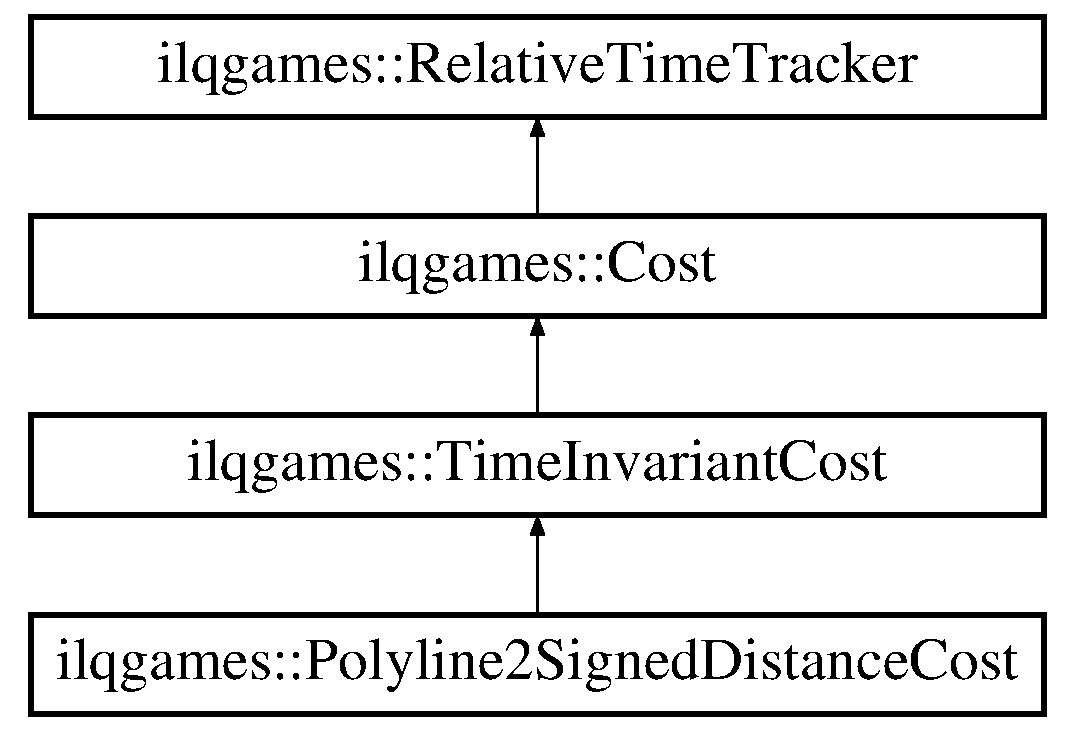
\includegraphics[height=4.000000cm]{classilqgames_1_1_polyline2_signed_distance_cost}
\end{center}
\end{figure}
\subsection*{Public Member Functions}
\begin{DoxyCompactItemize}
\item 
{\bfseries Polyline2\+Signed\+Distance\+Cost} (const \hyperlink{classilqgames_1_1_polyline2}{Polyline2} \&polyline, const std\+::pair$<$ Dimension, Dimension $>$ \&position\+\_\+idxs, const float nominal=0.\+0, bool oriented\+\_\+same\+\_\+as\+\_\+polyline=true, const std\+::string \&name=\char`\"{}\char`\"{})\hypertarget{classilqgames_1_1_polyline2_signed_distance_cost_a5eee356b43a0bbf0fdf2325e32e7f9a7}{}\label{classilqgames_1_1_polyline2_signed_distance_cost_a5eee356b43a0bbf0fdf2325e32e7f9a7}

\item 
float {\bfseries Evaluate} (const Vector\+Xf \&input) const \hypertarget{classilqgames_1_1_polyline2_signed_distance_cost_acf991d382328987f0757fa299d58f869}{}\label{classilqgames_1_1_polyline2_signed_distance_cost_acf991d382328987f0757fa299d58f869}

\item 
void {\bfseries Quadraticize} (const Vector\+Xf \&input, Matrix\+Xf $\ast$hess, Vector\+Xf $\ast$grad) const \hypertarget{classilqgames_1_1_polyline2_signed_distance_cost_a26d830bf62ef4b4e0827f8cbf779b21c}{}\label{classilqgames_1_1_polyline2_signed_distance_cost_a26d830bf62ef4b4e0827f8cbf779b21c}

\end{DoxyCompactItemize}
\subsection*{Additional Inherited Members}


\subsection{Detailed Description}


Definition at line 55 of file polyline2\+\_\+signed\+\_\+distance\+\_\+cost.\+h.



The documentation for this class was generated from the following files\+:\begin{DoxyCompactItemize}
\item 
/home/travis/build/\+H\+J\+Reachability/ilqgames/include/ilqgames/cost/polyline2\+\_\+signed\+\_\+distance\+\_\+cost.\+h\item 
/home/travis/build/\+H\+J\+Reachability/ilqgames/src/polyline2\+\_\+signed\+\_\+distance\+\_\+cost.\+cpp\end{DoxyCompactItemize}

\hypertarget{classilqgames_1_1_problem}{}\section{ilqgames\+:\+:Problem Class Reference}
\label{classilqgames_1_1_problem}\index{ilqgames\+::\+Problem@{ilqgames\+::\+Problem}}
Inheritance diagram for ilqgames\+:\+:Problem\+:\begin{figure}[H]
\begin{center}
\leavevmode
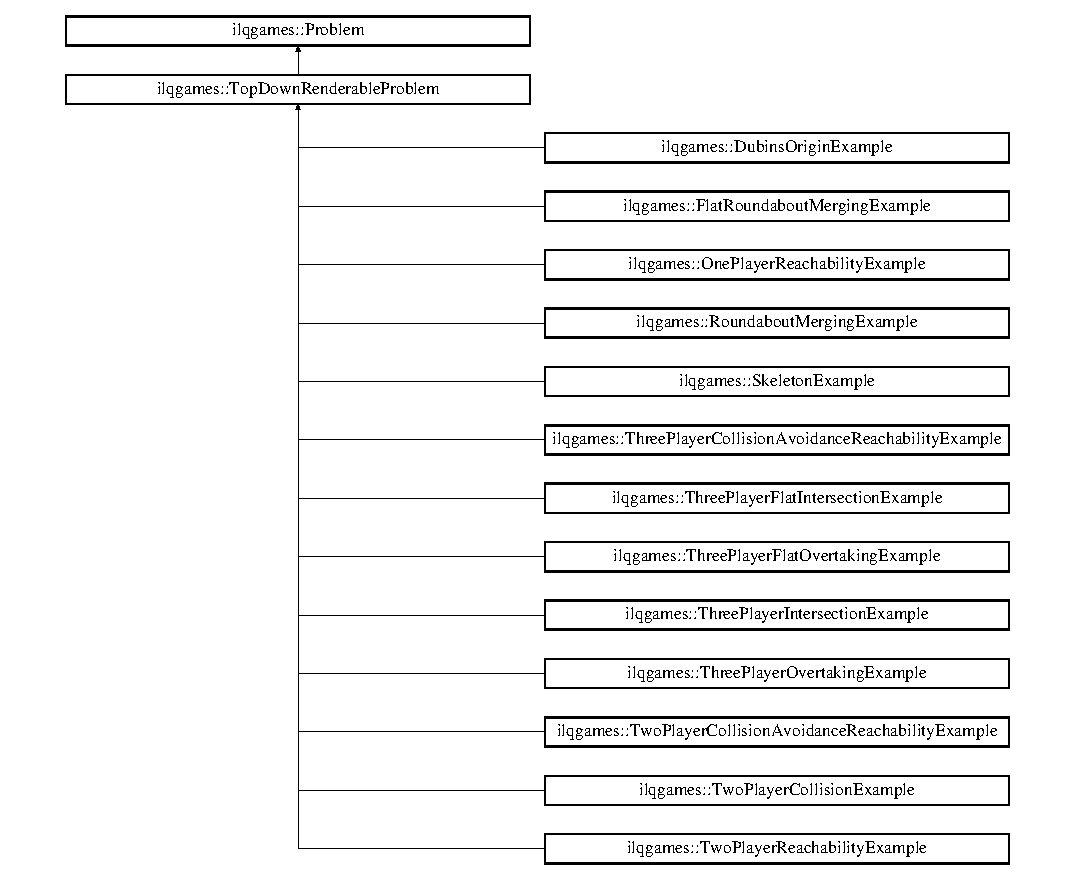
\includegraphics[height=10.623306cm]{classilqgames_1_1_problem}
\end{center}
\end{figure}
\subsection*{Public Member Functions}
\begin{DoxyCompactItemize}
\item 
std\+::shared\+\_\+ptr$<$ \hyperlink{classilqgames_1_1_solver_log}{Solver\+Log} $>$ {\bfseries Solve} (Time max\+\_\+runtime=std\+::numeric\+\_\+limits$<$ Time $>$\+::infinity())\hypertarget{classilqgames_1_1_problem_ab12b009e19551f6578af998789497927}{}\label{classilqgames_1_1_problem_ab12b009e19551f6578af998789497927}

\item 
void {\bfseries Reset\+Initial\+Time} (Time t0)\hypertarget{classilqgames_1_1_problem_a559eb8753ba5b82afeb6c69dd722a306}{}\label{classilqgames_1_1_problem_a559eb8753ba5b82afeb6c69dd722a306}

\item 
void {\bfseries Reset\+Initial\+State} (const Vector\+Xf \&x0)\hypertarget{classilqgames_1_1_problem_ac59f8a49b028baa3d72cb065d35b8193}{}\label{classilqgames_1_1_problem_ac59f8a49b028baa3d72cb065d35b8193}

\item 
virtual void {\bfseries Set\+Up\+Next\+Receding\+Horizon} (const Vector\+Xf \&x0, Time t0, Time planner\+\_\+runtime=0.\+1)\hypertarget{classilqgames_1_1_problem_adada206413bc775f078653da9c2ed033}{}\label{classilqgames_1_1_problem_adada206413bc775f078653da9c2ed033}

\item 
void {\bfseries Overwrite\+Solution} (const \hyperlink{structilqgames_1_1_operating_point}{Operating\+Point} \&operating\+\_\+point, const std\+::vector$<$ \hyperlink{structilqgames_1_1_strategy}{Strategy} $>$ \&strategies)\hypertarget{classilqgames_1_1_problem_a14744049661872191758323a4947f072}{}\label{classilqgames_1_1_problem_a14744049661872191758323a4947f072}

\item 
const \hyperlink{classilqgames_1_1_game_solver}{Game\+Solver} \& {\bfseries Solver} () const \hypertarget{classilqgames_1_1_problem_a5587e930ff86056f3ec7d2d01b43e4e5}{}\label{classilqgames_1_1_problem_a5587e930ff86056f3ec7d2d01b43e4e5}

\item 
const Vector\+Xf \& {\bfseries Initial\+State} () const \hypertarget{classilqgames_1_1_problem_a9b4d86b6f76908fdfc5ac82aae9320cb}{}\label{classilqgames_1_1_problem_a9b4d86b6f76908fdfc5ac82aae9320cb}

\item 
const \hyperlink{structilqgames_1_1_operating_point}{Operating\+Point} \& {\bfseries Current\+Operating\+Point} () const \hypertarget{classilqgames_1_1_problem_a49a937329474c57437592f09246c6517}{}\label{classilqgames_1_1_problem_a49a937329474c57437592f09246c6517}

\item 
const std\+::vector$<$ \hyperlink{structilqgames_1_1_strategy}{Strategy} $>$ \& {\bfseries Current\+Strategies} () const \hypertarget{classilqgames_1_1_problem_adb664a8d453bd4431789faf66d95a06a}{}\label{classilqgames_1_1_problem_adb664a8d453bd4431789faf66d95a06a}

\end{DoxyCompactItemize}
\subsection*{Protected Member Functions}
\begin{DoxyCompactItemize}
\item 
virtual std\+::shared\+\_\+ptr$<$ \hyperlink{classilqgames_1_1_solver_log}{Solver\+Log} $>$ {\bfseries Create\+New\+Log} () const \hypertarget{classilqgames_1_1_problem_a13d87495e055335f3da703909c435217}{}\label{classilqgames_1_1_problem_a13d87495e055335f3da703909c435217}

\end{DoxyCompactItemize}
\subsection*{Protected Attributes}
\begin{DoxyCompactItemize}
\item 
std\+::unique\+\_\+ptr$<$ \hyperlink{classilqgames_1_1_game_solver}{Game\+Solver} $>$ {\bfseries solver\+\_\+}\hypertarget{classilqgames_1_1_problem_aa14af0e2e063c99eefefd029d69dbf0d}{}\label{classilqgames_1_1_problem_aa14af0e2e063c99eefefd029d69dbf0d}

\item 
Vector\+Xf {\bfseries x0\+\_\+}\hypertarget{classilqgames_1_1_problem_a41236f0dfbc5eb6b1ddd08a5cc6555b3}{}\label{classilqgames_1_1_problem_a41236f0dfbc5eb6b1ddd08a5cc6555b3}

\item 
std\+::unique\+\_\+ptr$<$ \hyperlink{structilqgames_1_1_operating_point}{Operating\+Point} $>$ {\bfseries operating\+\_\+point\+\_\+}\hypertarget{classilqgames_1_1_problem_a2bb96299dbdc82440d6b90865ee9b2c1}{}\label{classilqgames_1_1_problem_a2bb96299dbdc82440d6b90865ee9b2c1}

\item 
std\+::unique\+\_\+ptr$<$ std\+::vector$<$ \hyperlink{structilqgames_1_1_strategy}{Strategy} $>$ $>$ {\bfseries strategies\+\_\+}\hypertarget{classilqgames_1_1_problem_a305d33a1e20a8ae63c0c581d562c7a64}{}\label{classilqgames_1_1_problem_a305d33a1e20a8ae63c0c581d562c7a64}

\end{DoxyCompactItemize}


\subsection{Detailed Description}


Definition at line 58 of file problem.\+h.



The documentation for this class was generated from the following files\+:\begin{DoxyCompactItemize}
\item 
/home/travis/build/\+H\+J\+Reachability/ilqgames/include/ilqgames/solver/problem.\+h\item 
/home/travis/build/\+H\+J\+Reachability/ilqgames/src/problem.\+cpp\end{DoxyCompactItemize}

\hypertarget{classilqgames_1_1_proximity_constraint}{}\section{ilqgames\+:\+:Proximity\+Constraint Class Reference}
\label{classilqgames_1_1_proximity_constraint}\index{ilqgames\+::\+Proximity\+Constraint@{ilqgames\+::\+Proximity\+Constraint}}
Inheritance diagram for ilqgames\+:\+:Proximity\+Constraint\+:\begin{figure}[H]
\begin{center}
\leavevmode
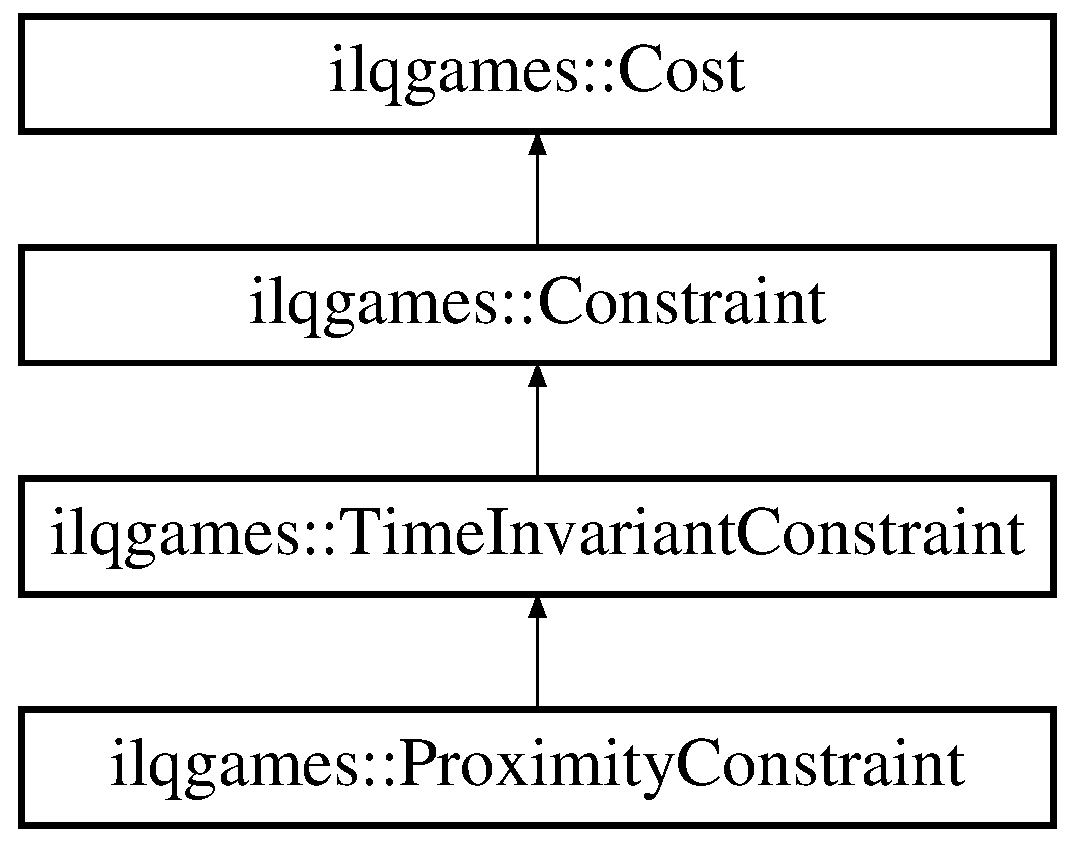
\includegraphics[height=4.000000cm]{classilqgames_1_1_proximity_constraint}
\end{center}
\end{figure}
\subsection*{Public Member Functions}
\begin{DoxyCompactItemize}
\item 
{\bfseries Proximity\+Constraint} (const std\+::pair$<$ Dimension, Dimension $>$ \&position\+\_\+idxs1, const std\+::pair$<$ Dimension, Dimension $>$ \&position\+\_\+idxs2, float threshold, bool inside=false, const std\+::string \&name=\char`\"{}\char`\"{})\hypertarget{classilqgames_1_1_proximity_constraint_a71159362756836048f230751764f1caa}{}\label{classilqgames_1_1_proximity_constraint_a71159362756836048f230751764f1caa}

\item 
bool {\bfseries Is\+Satisfied\+Level} (const Vector\+Xf \&input, float $\ast$level) const \hypertarget{classilqgames_1_1_proximity_constraint_aee644bf94f80bdb20b849828e428a062}{}\label{classilqgames_1_1_proximity_constraint_aee644bf94f80bdb20b849828e428a062}

\item 
void {\bfseries Quadraticize} (const Vector\+Xf \&input, Matrix\+Xf $\ast$hess, Vector\+Xf $\ast$grad) const \hypertarget{classilqgames_1_1_proximity_constraint_a8b9e59164c2be71572124872af9b7b79}{}\label{classilqgames_1_1_proximity_constraint_a8b9e59164c2be71572124872af9b7b79}

\end{DoxyCompactItemize}
\subsection*{Additional Inherited Members}


\subsection{Detailed Description}


Definition at line 59 of file proximity\+\_\+constraint.\+h.



The documentation for this class was generated from the following files\+:\begin{DoxyCompactItemize}
\item 
/home/travis/build/\+H\+J\+Reachability/ilqgames/include/ilqgames/constraint/proximity\+\_\+constraint.\+h\item 
/home/travis/build/\+H\+J\+Reachability/ilqgames/src/proximity\+\_\+constraint.\+cpp\end{DoxyCompactItemize}

\hypertarget{classilqgames_1_1_proximity_cost}{}\section{ilqgames\+:\+:Proximity\+Cost Class Reference}
\label{classilqgames_1_1_proximity_cost}\index{ilqgames\+::\+Proximity\+Cost@{ilqgames\+::\+Proximity\+Cost}}
Inheritance diagram for ilqgames\+:\+:Proximity\+Cost\+:\begin{figure}[H]
\begin{center}
\leavevmode
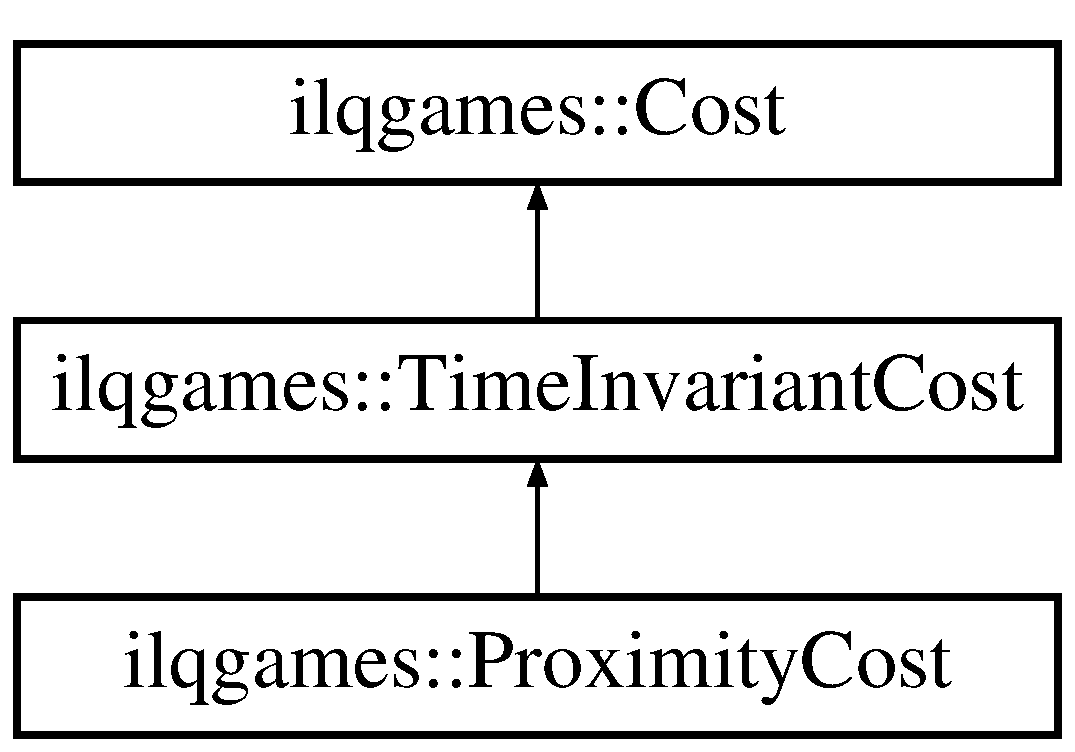
\includegraphics[height=3.000000cm]{classilqgames_1_1_proximity_cost}
\end{center}
\end{figure}
\subsection*{Public Member Functions}
\begin{DoxyCompactItemize}
\item 
{\bfseries Proximity\+Cost} (float weight, const std\+::pair$<$ Dimension, Dimension $>$ \&position\+\_\+idxs1, const std\+::pair$<$ Dimension, Dimension $>$ \&position\+\_\+idxs2, float threshold, const std\+::string \&name=\char`\"{}\char`\"{})\hypertarget{classilqgames_1_1_proximity_cost_a7b9f02baf7979aef9436f3f055fc8b81}{}\label{classilqgames_1_1_proximity_cost_a7b9f02baf7979aef9436f3f055fc8b81}

\item 
float {\bfseries Evaluate} (const Vector\+Xf \&input) const \hypertarget{classilqgames_1_1_proximity_cost_a0c5f46e7dba52dc6b1cb07c718b628ca}{}\label{classilqgames_1_1_proximity_cost_a0c5f46e7dba52dc6b1cb07c718b628ca}

\item 
void {\bfseries Quadraticize} (const Vector\+Xf \&input, Matrix\+Xf $\ast$hess, Vector\+Xf $\ast$grad=nullptr) const \hypertarget{classilqgames_1_1_proximity_cost_a3e71a4237039cc40c7a0d7fc439dc862}{}\label{classilqgames_1_1_proximity_cost_a3e71a4237039cc40c7a0d7fc439dc862}

\end{DoxyCompactItemize}
\subsection*{Additional Inherited Members}


\subsection{Detailed Description}


Definition at line 55 of file proximity\+\_\+cost.\+h.



The documentation for this class was generated from the following files\+:\begin{DoxyCompactItemize}
\item 
/home/travis/build/\+H\+J\+Reachability/ilqgames/include/ilqgames/cost/proximity\+\_\+cost.\+h\item 
/home/travis/build/\+H\+J\+Reachability/ilqgames/src/proximity\+\_\+cost.\+cpp\end{DoxyCompactItemize}

\hypertarget{classilqgames_1_1_quadratic_cost}{}\section{ilqgames\+:\+:Quadratic\+Cost Class Reference}
\label{classilqgames_1_1_quadratic_cost}\index{ilqgames\+::\+Quadratic\+Cost@{ilqgames\+::\+Quadratic\+Cost}}
Inheritance diagram for ilqgames\+:\+:Quadratic\+Cost\+:\begin{figure}[H]
\begin{center}
\leavevmode
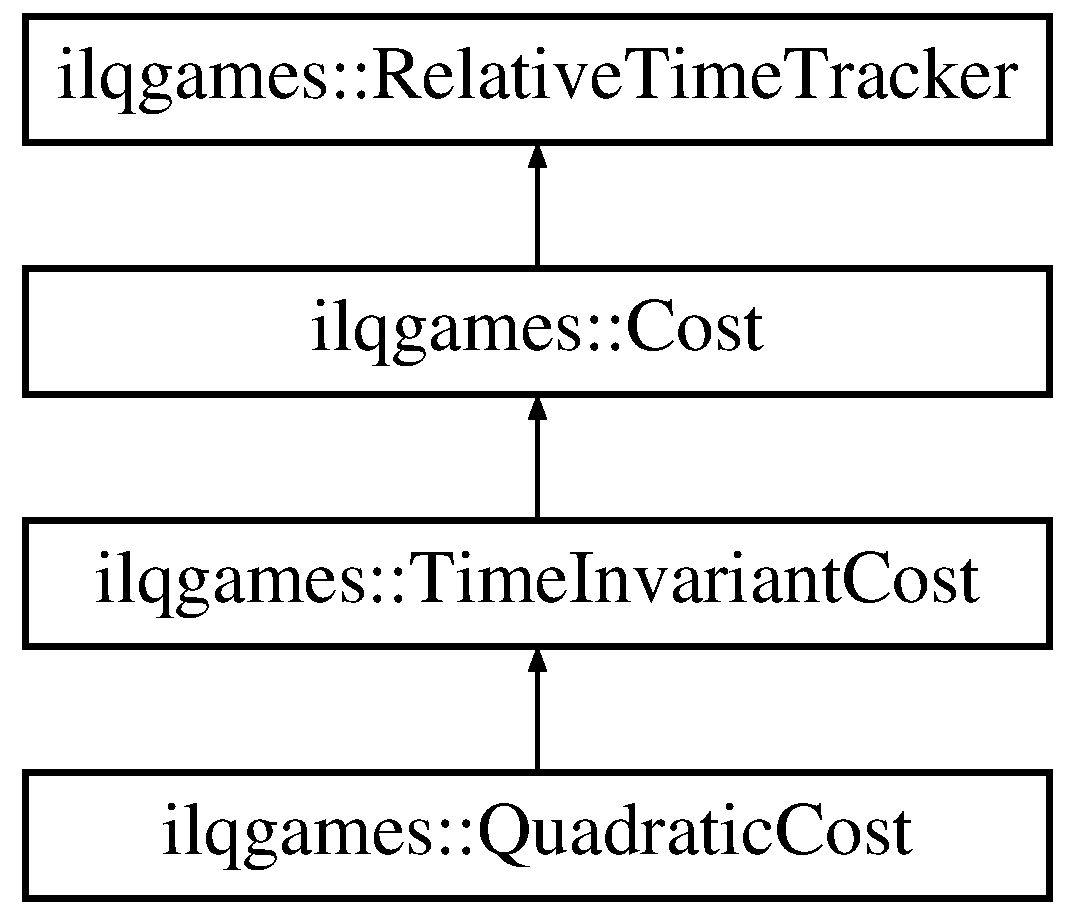
\includegraphics[height=4.000000cm]{classilqgames_1_1_quadratic_cost}
\end{center}
\end{figure}
\subsection*{Public Member Functions}
\begin{DoxyCompactItemize}
\item 
{\bfseries Quadratic\+Cost} (float weight, Dimension dim, float nominal=0.\+0, const std\+::string \&name=\char`\"{}\char`\"{})\hypertarget{classilqgames_1_1_quadratic_cost_a808c59c5dc19b77da62a8463f38cf4b1}{}\label{classilqgames_1_1_quadratic_cost_a808c59c5dc19b77da62a8463f38cf4b1}

\item 
float {\bfseries Evaluate} (const Vector\+Xf \&input) const \hypertarget{classilqgames_1_1_quadratic_cost_a2f1b56afdb011f212e7958e43f5601bc}{}\label{classilqgames_1_1_quadratic_cost_a2f1b56afdb011f212e7958e43f5601bc}

\item 
void {\bfseries Quadraticize} (const Vector\+Xf \&input, Matrix\+Xf $\ast$hess, Vector\+Xf $\ast$grad) const \hypertarget{classilqgames_1_1_quadratic_cost_aedfd8f1352bf30b1f4bf90d63dc38ce9}{}\label{classilqgames_1_1_quadratic_cost_aedfd8f1352bf30b1f4bf90d63dc38ce9}

\end{DoxyCompactItemize}
\subsection*{Additional Inherited Members}


\subsection{Detailed Description}


Definition at line 53 of file quadratic\+\_\+cost.\+h.



The documentation for this class was generated from the following files\+:\begin{DoxyCompactItemize}
\item 
/home/travis/build/\+H\+J\+Reachability/ilqgames/include/ilqgames/cost/quadratic\+\_\+cost.\+h\item 
/home/travis/build/\+H\+J\+Reachability/ilqgames/src/quadratic\+\_\+cost.\+cpp\end{DoxyCompactItemize}

\hypertarget{structilqgames_1_1_quadratic_cost_approximation}{}\section{ilqgames\+:\+:Quadratic\+Cost\+Approximation Struct Reference}
\label{structilqgames_1_1_quadratic_cost_approximation}\index{ilqgames\+::\+Quadratic\+Cost\+Approximation@{ilqgames\+::\+Quadratic\+Cost\+Approximation}}
\subsection*{Public Member Functions}
\begin{DoxyCompactItemize}
\item 
{\bfseries Quadratic\+Cost\+Approximation} (Dimension xdim, float regularization=0.\+0)\hypertarget{structilqgames_1_1_quadratic_cost_approximation_a0722ad542477052b0a489ead01165e16}{}\label{structilqgames_1_1_quadratic_cost_approximation_a0722ad542477052b0a489ead01165e16}

\end{DoxyCompactItemize}
\subsection*{Public Attributes}
\begin{DoxyCompactItemize}
\item 
\hyperlink{structilqgames_1_1_single_cost_approximation}{Single\+Cost\+Approximation} {\bfseries state}\hypertarget{structilqgames_1_1_quadratic_cost_approximation_a9a1ba94f8eb8f4c7bf22233feab63b15}{}\label{structilqgames_1_1_quadratic_cost_approximation_a9a1ba94f8eb8f4c7bf22233feab63b15}

\item 
Player\+Map$<$ \hyperlink{structilqgames_1_1_single_cost_approximation}{Single\+Cost\+Approximation} $>$ {\bfseries control}\hypertarget{structilqgames_1_1_quadratic_cost_approximation_af5713bb905716d24ebdd581d48add80a}{}\label{structilqgames_1_1_quadratic_cost_approximation_af5713bb905716d24ebdd581d48add80a}

\end{DoxyCompactItemize}


\subsection{Detailed Description}


Definition at line 78 of file quadratic\+\_\+cost\+\_\+approximation.\+h.



The documentation for this struct was generated from the following file\+:\begin{DoxyCompactItemize}
\item 
/home/travis/build/\+H\+J\+Reachability/ilqgames/include/ilqgames/utils/quadratic\+\_\+cost\+\_\+approximation.\+h\end{DoxyCompactItemize}

\hypertarget{classilqgames_1_1_quadratic_difference_cost}{}\section{ilqgames\+:\+:Quadratic\+Difference\+Cost Class Reference}
\label{classilqgames_1_1_quadratic_difference_cost}\index{ilqgames\+::\+Quadratic\+Difference\+Cost@{ilqgames\+::\+Quadratic\+Difference\+Cost}}
Inheritance diagram for ilqgames\+:\+:Quadratic\+Difference\+Cost\+:\begin{figure}[H]
\begin{center}
\leavevmode
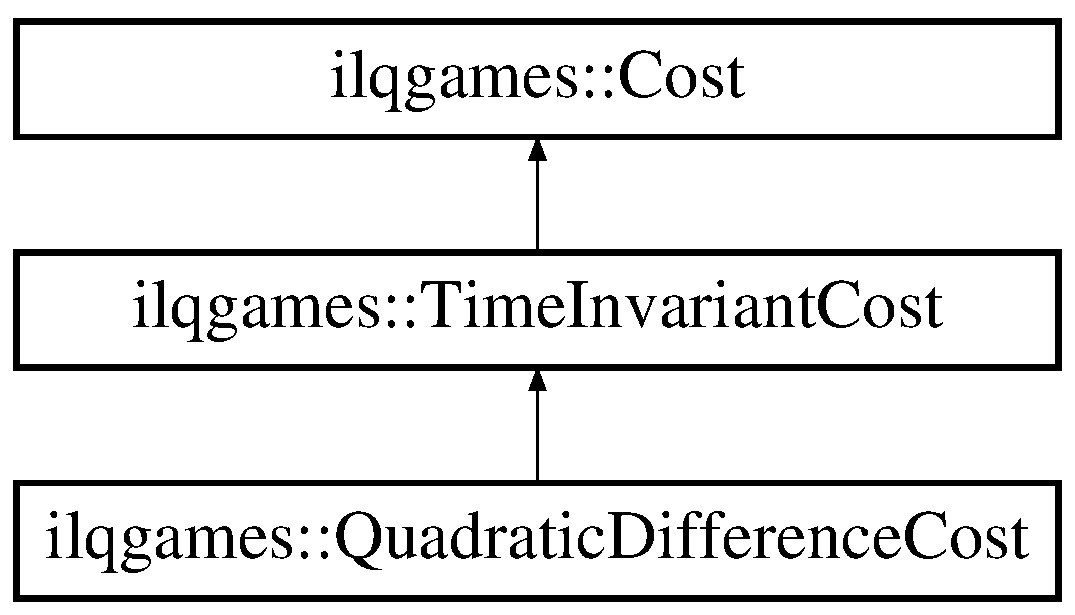
\includegraphics[height=3.000000cm]{classilqgames_1_1_quadratic_difference_cost}
\end{center}
\end{figure}
\subsection*{Public Member Functions}
\begin{DoxyCompactItemize}
\item 
{\bfseries Quadratic\+Difference\+Cost} (float weight, const std\+::vector$<$ Dimension $>$ \&dims1, const std\+::vector$<$ Dimension $>$ \&dims2, const std\+::string \&name=\char`\"{}\char`\"{})\hypertarget{classilqgames_1_1_quadratic_difference_cost_afe5dfe4c10ff8fd995f9f0313860883e}{}\label{classilqgames_1_1_quadratic_difference_cost_afe5dfe4c10ff8fd995f9f0313860883e}

\item 
float {\bfseries Evaluate} (const Vector\+Xf \&input) const \hypertarget{classilqgames_1_1_quadratic_difference_cost_adc6943c8b7dee651b61406e1276ecbca}{}\label{classilqgames_1_1_quadratic_difference_cost_adc6943c8b7dee651b61406e1276ecbca}

\item 
void {\bfseries Quadraticize} (const Vector\+Xf \&input, Matrix\+Xf $\ast$hess, Vector\+Xf $\ast$grad) const \hypertarget{classilqgames_1_1_quadratic_difference_cost_a10d67623d9b82bf350a7ff98bda102e2}{}\label{classilqgames_1_1_quadratic_difference_cost_a10d67623d9b82bf350a7ff98bda102e2}

\end{DoxyCompactItemize}
\subsection*{Additional Inherited Members}


\subsection{Detailed Description}


Definition at line 54 of file quadratic\+\_\+difference\+\_\+cost.\+h.



The documentation for this class was generated from the following files\+:\begin{DoxyCompactItemize}
\item 
/home/travis/build/\+H\+J\+Reachability/ilqgames/include/ilqgames/cost/quadratic\+\_\+difference\+\_\+cost.\+h\item 
/home/travis/build/\+H\+J\+Reachability/ilqgames/src/quadratic\+\_\+difference\+\_\+cost.\+cpp\end{DoxyCompactItemize}

\hypertarget{classilqgames_1_1_quadratic_norm_cost}{}\section{ilqgames\+:\+:Quadratic\+Norm\+Cost Class Reference}
\label{classilqgames_1_1_quadratic_norm_cost}\index{ilqgames\+::\+Quadratic\+Norm\+Cost@{ilqgames\+::\+Quadratic\+Norm\+Cost}}
Inheritance diagram for ilqgames\+:\+:Quadratic\+Norm\+Cost\+:\begin{figure}[H]
\begin{center}
\leavevmode
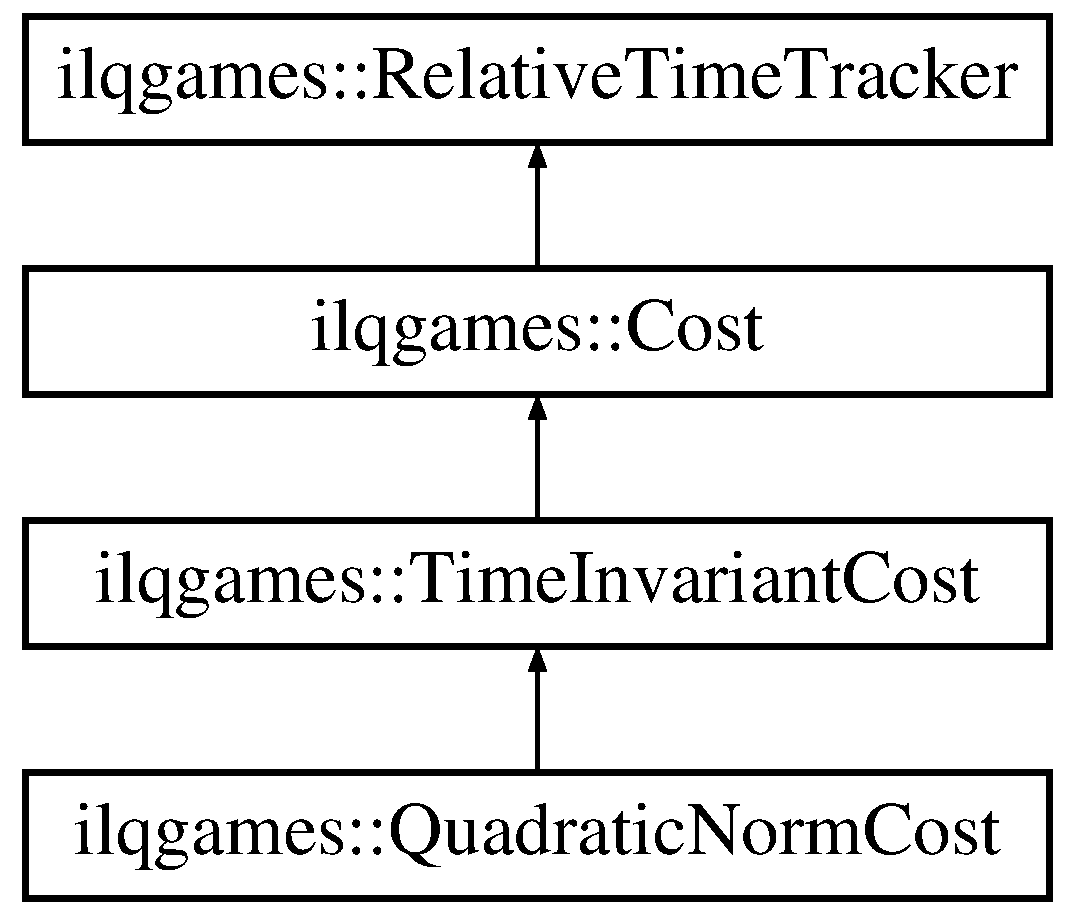
\includegraphics[height=3.000000cm]{classilqgames_1_1_quadratic_norm_cost}
\end{center}
\end{figure}
\subsection*{Public Member Functions}
\begin{DoxyCompactItemize}
\item 
{\bfseries Quadratic\+Norm\+Cost} (float weight, const std\+::pair$<$ Dimension, Dimension $>$ \&dims, float nominal=0.\+0, const std\+::string \&name=\char`\"{}\char`\"{})\hypertarget{classilqgames_1_1_quadratic_norm_cost_a3a8704f72c0d6b4d968bd4e857d53c44}{}\label{classilqgames_1_1_quadratic_norm_cost_a3a8704f72c0d6b4d968bd4e857d53c44}

\item 
float {\bfseries Evaluate} (const Vector\+Xf \&input) const \hypertarget{classilqgames_1_1_quadratic_norm_cost_a627c6954a3c91608f09d54050b0c9a0d}{}\label{classilqgames_1_1_quadratic_norm_cost_a627c6954a3c91608f09d54050b0c9a0d}

\item 
void {\bfseries Quadraticize} (const Vector\+Xf \&input, Matrix\+Xf $\ast$hess, Vector\+Xf $\ast$grad) const \hypertarget{classilqgames_1_1_quadratic_norm_cost_af497480714a9fc5480983f28521d1ad0}{}\label{classilqgames_1_1_quadratic_norm_cost_af497480714a9fc5480983f28521d1ad0}

\end{DoxyCompactItemize}
\subsection*{Additional Inherited Members}


\subsection{Detailed Description}


Definition at line 56 of file quadratic\+\_\+norm\+\_\+cost.\+h.



The documentation for this class was generated from the following files\+:\begin{DoxyCompactItemize}
\item 
/home/travis/build/\+H\+J\+Reachability/ilqgames/include/ilqgames/cost/quadratic\+\_\+norm\+\_\+cost.\+h\item 
/home/travis/build/\+H\+J\+Reachability/ilqgames/src/quadratic\+\_\+norm\+\_\+cost.\+cpp\end{DoxyCompactItemize}

\hypertarget{classilqgames_1_1_quadratic_polyline2_cost}{}\section{ilqgames\+:\+:Quadratic\+Polyline2\+Cost Class Reference}
\label{classilqgames_1_1_quadratic_polyline2_cost}\index{ilqgames\+::\+Quadratic\+Polyline2\+Cost@{ilqgames\+::\+Quadratic\+Polyline2\+Cost}}
Inheritance diagram for ilqgames\+:\+:Quadratic\+Polyline2\+Cost\+:\begin{figure}[H]
\begin{center}
\leavevmode
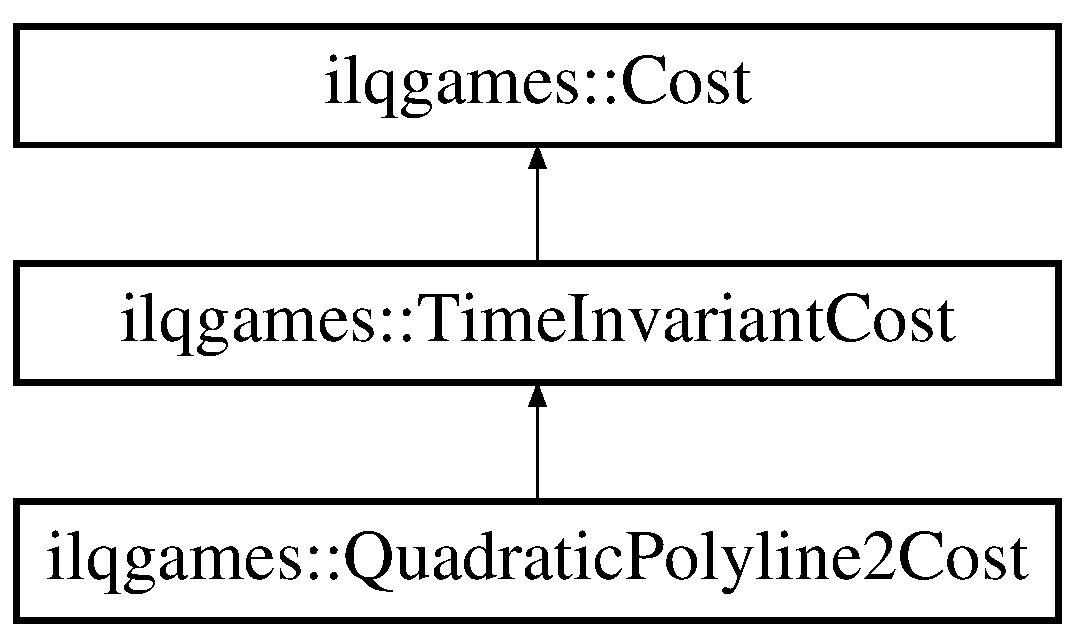
\includegraphics[height=4.000000cm]{classilqgames_1_1_quadratic_polyline2_cost}
\end{center}
\end{figure}
\subsection*{Public Member Functions}
\begin{DoxyCompactItemize}
\item 
{\bfseries Quadratic\+Polyline2\+Cost} (float weight, const \hyperlink{classilqgames_1_1_polyline2}{Polyline2} \&polyline, const std\+::pair$<$ Dimension, Dimension $>$ \&position\+\_\+idxs, const std\+::string \&name=\char`\"{}\char`\"{})\hypertarget{classilqgames_1_1_quadratic_polyline2_cost_a3385f76e02730e44a9eb5b9ddfff7797}{}\label{classilqgames_1_1_quadratic_polyline2_cost_a3385f76e02730e44a9eb5b9ddfff7797}

\item 
float {\bfseries Evaluate} (const Vector\+Xf \&input) const \hypertarget{classilqgames_1_1_quadratic_polyline2_cost_a5925c379ffbb7ce5aa10ce50f230540a}{}\label{classilqgames_1_1_quadratic_polyline2_cost_a5925c379ffbb7ce5aa10ce50f230540a}

\item 
void {\bfseries Quadraticize} (const Vector\+Xf \&input, Matrix\+Xf $\ast$hess, Vector\+Xf $\ast$grad) const \hypertarget{classilqgames_1_1_quadratic_polyline2_cost_a197ff1f9167de29c3961f9b68fe2636b}{}\label{classilqgames_1_1_quadratic_polyline2_cost_a197ff1f9167de29c3961f9b68fe2636b}

\end{DoxyCompactItemize}
\subsection*{Additional Inherited Members}


\subsection{Detailed Description}


Definition at line 55 of file quadratic\+\_\+polyline2\+\_\+cost.\+h.



The documentation for this class was generated from the following files\+:\begin{DoxyCompactItemize}
\item 
/home/travis/build/\+H\+J\+Reachability/ilqgames/include/ilqgames/cost/quadratic\+\_\+polyline2\+\_\+cost.\+h\item 
/home/travis/build/\+H\+J\+Reachability/ilqgames/src/quadratic\+\_\+polyline2\+\_\+cost.\+cpp\end{DoxyCompactItemize}

\hypertarget{classilqgames_1_1_roundabout_merging_example}{}\section{ilqgames\+:\+:Roundabout\+Merging\+Example Class Reference}
\label{classilqgames_1_1_roundabout_merging_example}\index{ilqgames\+::\+Roundabout\+Merging\+Example@{ilqgames\+::\+Roundabout\+Merging\+Example}}
Inheritance diagram for ilqgames\+:\+:Roundabout\+Merging\+Example\+:\begin{figure}[H]
\begin{center}
\leavevmode
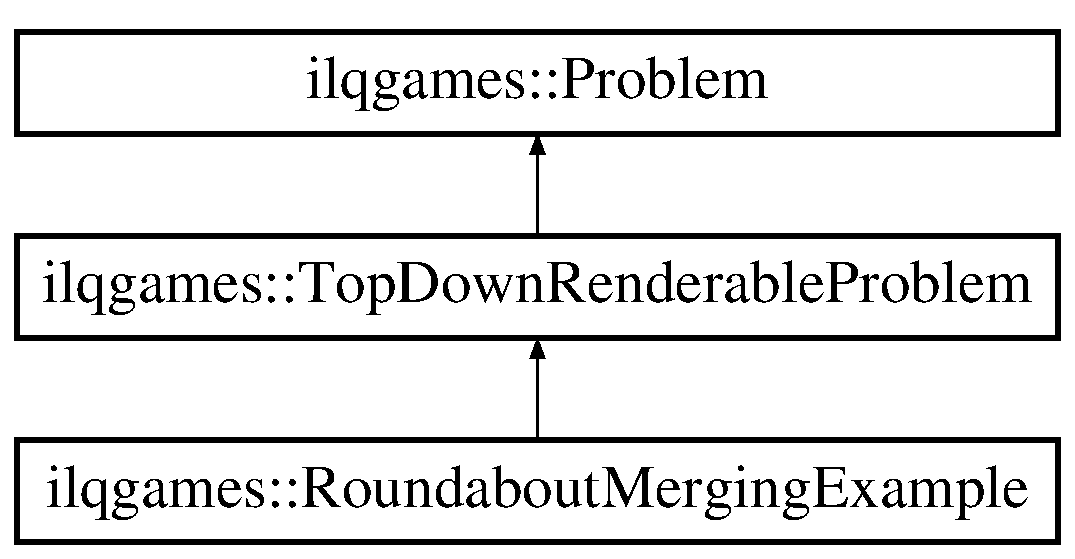
\includegraphics[height=3.000000cm]{classilqgames_1_1_roundabout_merging_example}
\end{center}
\end{figure}
\subsection*{Public Member Functions}
\begin{DoxyCompactItemize}
\item 
{\bfseries Roundabout\+Merging\+Example} (const \hyperlink{structilqgames_1_1_solver_params}{Solver\+Params} \&params)\hypertarget{classilqgames_1_1_roundabout_merging_example_a9a36e72c360e99825bccf1de9ad54cef}{}\label{classilqgames_1_1_roundabout_merging_example_a9a36e72c360e99825bccf1de9ad54cef}

\item 
std\+::vector$<$ float $>$ {\bfseries Xs} (const Vector\+Xf \&x) const \hypertarget{classilqgames_1_1_roundabout_merging_example_adbe4b0b31b690b4a6bea6a5677f2db3f}{}\label{classilqgames_1_1_roundabout_merging_example_adbe4b0b31b690b4a6bea6a5677f2db3f}

\item 
std\+::vector$<$ float $>$ {\bfseries Ys} (const Vector\+Xf \&x) const \hypertarget{classilqgames_1_1_roundabout_merging_example_ab2f826a33b86e86199327f78f7572245}{}\label{classilqgames_1_1_roundabout_merging_example_ab2f826a33b86e86199327f78f7572245}

\item 
std\+::vector$<$ float $>$ {\bfseries Thetas} (const Vector\+Xf \&x) const \hypertarget{classilqgames_1_1_roundabout_merging_example_a3f8e894816106634504dd2d2e75cc73a}{}\label{classilqgames_1_1_roundabout_merging_example_a3f8e894816106634504dd2d2e75cc73a}

\end{DoxyCompactItemize}
\subsection*{Additional Inherited Members}


\subsection{Detailed Description}


Definition at line 52 of file roundabout\+\_\+merging\+\_\+example.\+h.



The documentation for this class was generated from the following files\+:\begin{DoxyCompactItemize}
\item 
/home/travis/build/\+H\+J\+Reachability/ilqgames/include/ilqgames/examples/roundabout\+\_\+merging\+\_\+example.\+h\item 
/home/travis/build/\+H\+J\+Reachability/ilqgames/src/roundabout\+\_\+merging\+\_\+example.\+cpp\end{DoxyCompactItemize}

\hypertarget{classilqgames_1_1_route_progress_cost}{}\section{ilqgames\+:\+:Route\+Progress\+Cost Class Reference}
\label{classilqgames_1_1_route_progress_cost}\index{ilqgames\+::\+Route\+Progress\+Cost@{ilqgames\+::\+Route\+Progress\+Cost}}
Inheritance diagram for ilqgames\+:\+:Route\+Progress\+Cost\+:\begin{figure}[H]
\begin{center}
\leavevmode
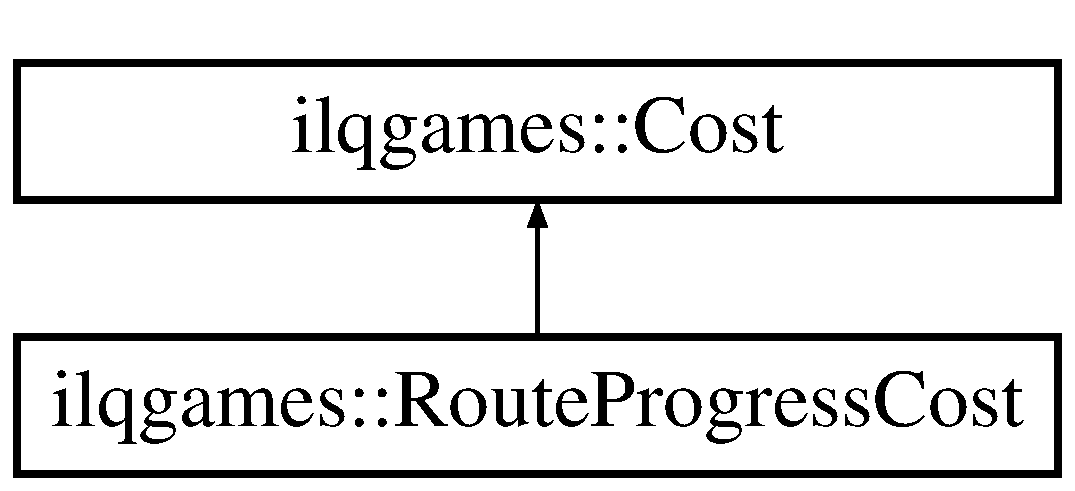
\includegraphics[height=3.000000cm]{classilqgames_1_1_route_progress_cost}
\end{center}
\end{figure}
\subsection*{Public Member Functions}
\begin{DoxyCompactItemize}
\item 
{\bfseries Route\+Progress\+Cost} (float weight, float nominal\+\_\+speed, const \hyperlink{classilqgames_1_1_polyline2}{Polyline2} \&polyline, const std\+::pair$<$ Dimension, Dimension $>$ \&position\+\_\+idxs, const std\+::string \&name=\char`\"{}\char`\"{}, float initial\+\_\+route\+\_\+pos=0.\+0)\hypertarget{classilqgames_1_1_route_progress_cost_a9bc119604ce84627367f7e943e28a90d}{}\label{classilqgames_1_1_route_progress_cost_a9bc119604ce84627367f7e943e28a90d}

\item 
float {\bfseries Evaluate} (Time t, const Vector\+Xf \&input) const \hypertarget{classilqgames_1_1_route_progress_cost_a93a76046fac60030e3f8767c0b8efea0}{}\label{classilqgames_1_1_route_progress_cost_a93a76046fac60030e3f8767c0b8efea0}

\item 
void {\bfseries Quadraticize} (Time t, const Vector\+Xf \&input, Matrix\+Xf $\ast$hess, Vector\+Xf $\ast$grad) const \hypertarget{classilqgames_1_1_route_progress_cost_a51ac030f155eafcf5c7f52ee7220ec4f}{}\label{classilqgames_1_1_route_progress_cost_a51ac030f155eafcf5c7f52ee7220ec4f}

\end{DoxyCompactItemize}
\subsection*{Additional Inherited Members}


\subsection{Detailed Description}


Definition at line 56 of file route\+\_\+progress\+\_\+cost.\+h.



The documentation for this class was generated from the following files\+:\begin{DoxyCompactItemize}
\item 
/home/travis/build/\+H\+J\+Reachability/ilqgames/include/ilqgames/cost/route\+\_\+progress\+\_\+cost.\+h\item 
/home/travis/build/\+H\+J\+Reachability/ilqgames/src/route\+\_\+progress\+\_\+cost.\+cpp\end{DoxyCompactItemize}

\hypertarget{classilqgames_1_1_semiquadratic_cost}{}\section{ilqgames\+:\+:Semiquadratic\+Cost Class Reference}
\label{classilqgames_1_1_semiquadratic_cost}\index{ilqgames\+::\+Semiquadratic\+Cost@{ilqgames\+::\+Semiquadratic\+Cost}}
Inheritance diagram for ilqgames\+:\+:Semiquadratic\+Cost\+:\begin{figure}[H]
\begin{center}
\leavevmode
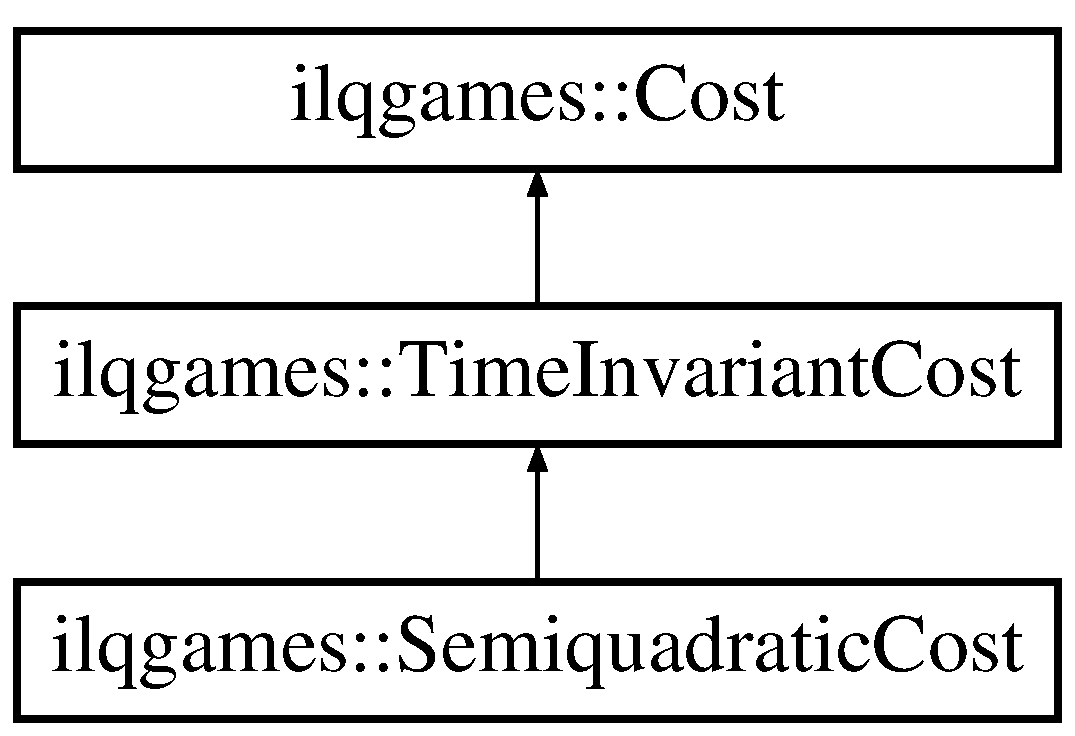
\includegraphics[height=3.000000cm]{classilqgames_1_1_semiquadratic_cost}
\end{center}
\end{figure}
\subsection*{Public Member Functions}
\begin{DoxyCompactItemize}
\item 
{\bfseries Semiquadratic\+Cost} (float weight, Dimension dim, float threshold, bool oriented\+\_\+right, const std\+::string \&name=\char`\"{}\char`\"{})\hypertarget{classilqgames_1_1_semiquadratic_cost_a007448675efe7997d373403c08eaaff1}{}\label{classilqgames_1_1_semiquadratic_cost_a007448675efe7997d373403c08eaaff1}

\item 
float {\bfseries Evaluate} (const Vector\+Xf \&input) const \hypertarget{classilqgames_1_1_semiquadratic_cost_a1c4e3c92a5f72383d72c4d8e3191c26c}{}\label{classilqgames_1_1_semiquadratic_cost_a1c4e3c92a5f72383d72c4d8e3191c26c}

\item 
void {\bfseries Quadraticize} (const Vector\+Xf \&input, Matrix\+Xf $\ast$hess, Vector\+Xf $\ast$grad) const \hypertarget{classilqgames_1_1_semiquadratic_cost_a70151cab48cd670278704948c144cda6}{}\label{classilqgames_1_1_semiquadratic_cost_a70151cab48cd670278704948c144cda6}

\end{DoxyCompactItemize}
\subsection*{Additional Inherited Members}


\subsection{Detailed Description}


Definition at line 55 of file semiquadratic\+\_\+cost.\+h.



The documentation for this class was generated from the following files\+:\begin{DoxyCompactItemize}
\item 
/home/travis/build/\+H\+J\+Reachability/ilqgames/include/ilqgames/cost/semiquadratic\+\_\+cost.\+h\item 
/home/travis/build/\+H\+J\+Reachability/ilqgames/src/semiquadratic\+\_\+cost.\+cpp\end{DoxyCompactItemize}

\hypertarget{classilqgames_1_1_semiquadratic_norm_cost}{}\section{ilqgames\+:\+:Semiquadratic\+Norm\+Cost Class Reference}
\label{classilqgames_1_1_semiquadratic_norm_cost}\index{ilqgames\+::\+Semiquadratic\+Norm\+Cost@{ilqgames\+::\+Semiquadratic\+Norm\+Cost}}
Inheritance diagram for ilqgames\+:\+:Semiquadratic\+Norm\+Cost\+:\begin{figure}[H]
\begin{center}
\leavevmode
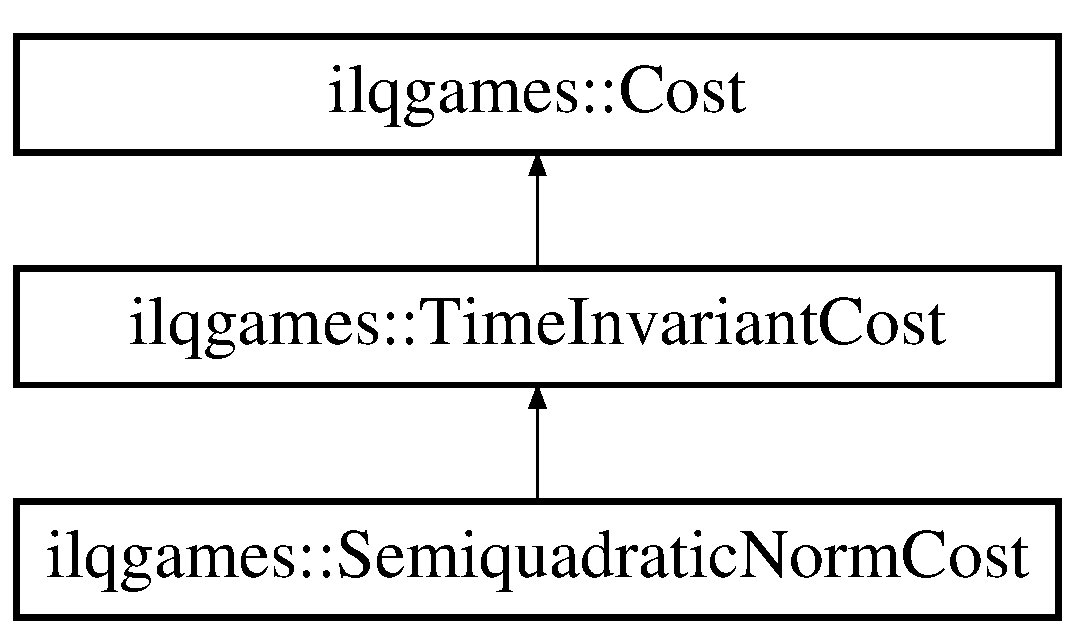
\includegraphics[height=3.000000cm]{classilqgames_1_1_semiquadratic_norm_cost}
\end{center}
\end{figure}
\subsection*{Public Member Functions}
\begin{DoxyCompactItemize}
\item 
{\bfseries Semiquadratic\+Norm\+Cost} (float weight, const std\+::pair$<$ Dimension, Dimension $>$ \&dims, float threshold, bool oriented\+\_\+right, const std\+::string \&name=\char`\"{}\char`\"{})\hypertarget{classilqgames_1_1_semiquadratic_norm_cost_a1f2f9189770f6128afe12d3a3aed0a7a}{}\label{classilqgames_1_1_semiquadratic_norm_cost_a1f2f9189770f6128afe12d3a3aed0a7a}

\item 
float {\bfseries Evaluate} (const Vector\+Xf \&input) const \hypertarget{classilqgames_1_1_semiquadratic_norm_cost_af8df2f58dc246d0d450f53f4fd9086f2}{}\label{classilqgames_1_1_semiquadratic_norm_cost_af8df2f58dc246d0d450f53f4fd9086f2}

\item 
void {\bfseries Quadraticize} (const Vector\+Xf \&input, Matrix\+Xf $\ast$hess, Vector\+Xf $\ast$grad=nullptr) const \hypertarget{classilqgames_1_1_semiquadratic_norm_cost_ad35dfe1f0729ca73bd68edd3bc23a114}{}\label{classilqgames_1_1_semiquadratic_norm_cost_ad35dfe1f0729ca73bd68edd3bc23a114}

\end{DoxyCompactItemize}
\subsection*{Additional Inherited Members}


\subsection{Detailed Description}


Definition at line 57 of file semiquadratic\+\_\+norm\+\_\+cost.\+h.



The documentation for this class was generated from the following files\+:\begin{DoxyCompactItemize}
\item 
/home/travis/build/\+H\+J\+Reachability/ilqgames/include/ilqgames/cost/semiquadratic\+\_\+norm\+\_\+cost.\+h\item 
/home/travis/build/\+H\+J\+Reachability/ilqgames/src/semiquadratic\+\_\+norm\+\_\+cost.\+cpp\end{DoxyCompactItemize}

\hypertarget{classilqgames_1_1_semiquadratic_polyline2_cost}{}\section{ilqgames\+:\+:Semiquadratic\+Polyline2\+Cost Class Reference}
\label{classilqgames_1_1_semiquadratic_polyline2_cost}\index{ilqgames\+::\+Semiquadratic\+Polyline2\+Cost@{ilqgames\+::\+Semiquadratic\+Polyline2\+Cost}}
Inheritance diagram for ilqgames\+:\+:Semiquadratic\+Polyline2\+Cost\+:\begin{figure}[H]
\begin{center}
\leavevmode
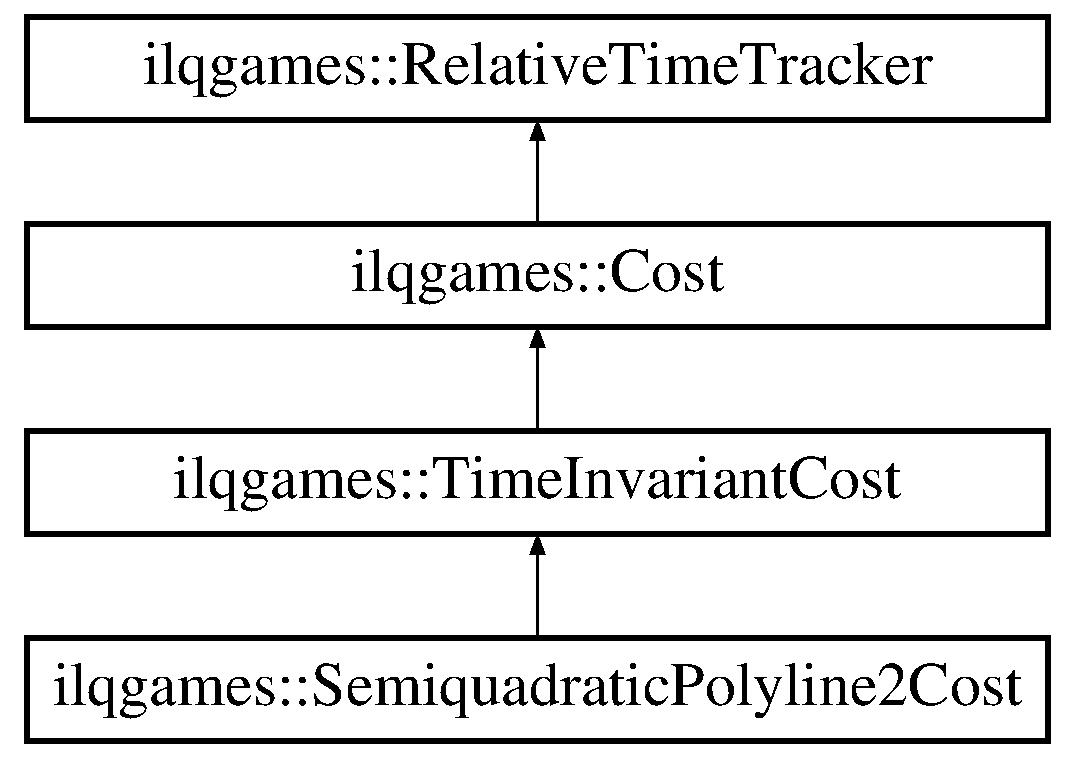
\includegraphics[height=4.000000cm]{classilqgames_1_1_semiquadratic_polyline2_cost}
\end{center}
\end{figure}
\subsection*{Public Member Functions}
\begin{DoxyCompactItemize}
\item 
{\bfseries Semiquadratic\+Polyline2\+Cost} (float weight, const \hyperlink{classilqgames_1_1_polyline2}{Polyline2} \&polyline, const std\+::pair$<$ Dimension, Dimension $>$ \&position\+\_\+idxs, float threshold, bool oriented\+\_\+right, const std\+::string \&name=\char`\"{}\char`\"{})\hypertarget{classilqgames_1_1_semiquadratic_polyline2_cost_a7e928410aef0e930024890fb519b1290}{}\label{classilqgames_1_1_semiquadratic_polyline2_cost_a7e928410aef0e930024890fb519b1290}

\item 
float {\bfseries Evaluate} (const Vector\+Xf \&input) const \hypertarget{classilqgames_1_1_semiquadratic_polyline2_cost_abe1063a923c02e53e3512b4de85539b8}{}\label{classilqgames_1_1_semiquadratic_polyline2_cost_abe1063a923c02e53e3512b4de85539b8}

\item 
void {\bfseries Quadraticize} (const Vector\+Xf \&input, Matrix\+Xf $\ast$hess, Vector\+Xf $\ast$grad) const \hypertarget{classilqgames_1_1_semiquadratic_polyline2_cost_a74b1ce98fe98f50560f21751a7c855f2}{}\label{classilqgames_1_1_semiquadratic_polyline2_cost_a74b1ce98fe98f50560f21751a7c855f2}

\end{DoxyCompactItemize}
\subsection*{Additional Inherited Members}


\subsection{Detailed Description}


Definition at line 55 of file semiquadratic\+\_\+polyline2\+\_\+cost.\+h.



The documentation for this class was generated from the following files\+:\begin{DoxyCompactItemize}
\item 
/home/travis/build/\+H\+J\+Reachability/ilqgames/include/ilqgames/cost/semiquadratic\+\_\+polyline2\+\_\+cost.\+h\item 
/home/travis/build/\+H\+J\+Reachability/ilqgames/src/semiquadratic\+\_\+polyline2\+\_\+cost.\+cpp\end{DoxyCompactItemize}

\hypertarget{classilqgames_1_1_signed_distance_cost}{}\section{ilqgames\+:\+:Signed\+Distance\+Cost Class Reference}
\label{classilqgames_1_1_signed_distance_cost}\index{ilqgames\+::\+Signed\+Distance\+Cost@{ilqgames\+::\+Signed\+Distance\+Cost}}
Inheritance diagram for ilqgames\+:\+:Signed\+Distance\+Cost\+:\begin{figure}[H]
\begin{center}
\leavevmode
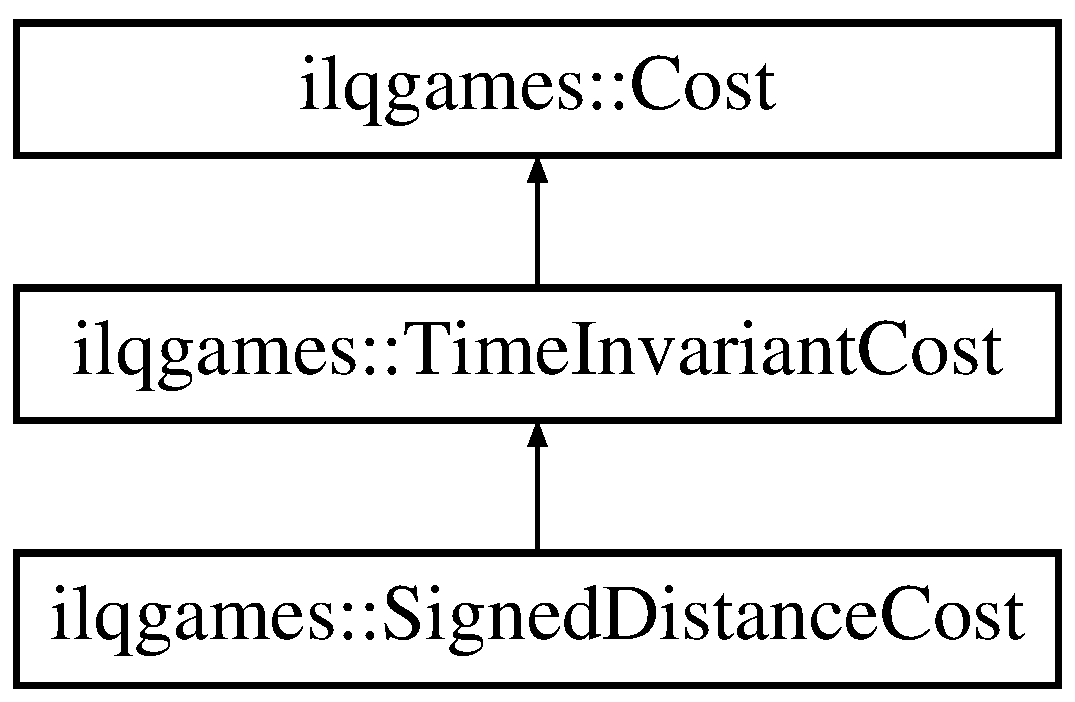
\includegraphics[height=3.000000cm]{classilqgames_1_1_signed_distance_cost}
\end{center}
\end{figure}
\subsection*{Public Member Functions}
\begin{DoxyCompactItemize}
\item 
{\bfseries Signed\+Distance\+Cost} (const std\+::pair$<$ Dimension, Dimension $>$ \&dims1, const std\+::pair$<$ Dimension, Dimension $>$ \&dims2, float nominal=0.\+0, bool less\+\_\+is\+\_\+positive=true, const std\+::string \&name=\char`\"{}\char`\"{})\hypertarget{classilqgames_1_1_signed_distance_cost_acaf7384522a5bbb6a282b93ed0c7a096}{}\label{classilqgames_1_1_signed_distance_cost_acaf7384522a5bbb6a282b93ed0c7a096}

\item 
float {\bfseries Evaluate} (const Vector\+Xf \&input) const \hypertarget{classilqgames_1_1_signed_distance_cost_a9694c04cf297f78923eefa0b6d472595}{}\label{classilqgames_1_1_signed_distance_cost_a9694c04cf297f78923eefa0b6d472595}

\item 
void {\bfseries Quadraticize} (const Vector\+Xf \&input, Matrix\+Xf $\ast$hess, Vector\+Xf $\ast$grad) const \hypertarget{classilqgames_1_1_signed_distance_cost_a655aa06d6933385c802895025ab94162}{}\label{classilqgames_1_1_signed_distance_cost_a655aa06d6933385c802895025ab94162}

\end{DoxyCompactItemize}
\subsection*{Additional Inherited Members}


\subsection{Detailed Description}


Definition at line 53 of file signed\+\_\+distance\+\_\+cost.\+h.



The documentation for this class was generated from the following files\+:\begin{DoxyCompactItemize}
\item 
/home/travis/build/\+H\+J\+Reachability/ilqgames/include/ilqgames/cost/signed\+\_\+distance\+\_\+cost.\+h\item 
/home/travis/build/\+H\+J\+Reachability/ilqgames/src/signed\+\_\+distance\+\_\+cost.\+cpp\end{DoxyCompactItemize}

\hypertarget{structilqgames_1_1_single_cost_approximation}{}\section{ilqgames\+:\+:Single\+Cost\+Approximation Struct Reference}
\label{structilqgames_1_1_single_cost_approximation}\index{ilqgames\+::\+Single\+Cost\+Approximation@{ilqgames\+::\+Single\+Cost\+Approximation}}
\subsection*{Public Member Functions}
\begin{DoxyCompactItemize}
\item 
{\bfseries Single\+Cost\+Approximation} (const Matrix\+Xf \&hessian, const Vector\+Xf \&gradient)\hypertarget{structilqgames_1_1_single_cost_approximation_a33cb225c90ccecd41aeb0bb21e6f8205}{}\label{structilqgames_1_1_single_cost_approximation_a33cb225c90ccecd41aeb0bb21e6f8205}

\item 
{\bfseries Single\+Cost\+Approximation} (Dimension dim, float regularization=0.\+0)\hypertarget{structilqgames_1_1_single_cost_approximation_af0031622bb059b5728e48d28310563d5}{}\label{structilqgames_1_1_single_cost_approximation_af0031622bb059b5728e48d28310563d5}

\end{DoxyCompactItemize}
\subsection*{Public Attributes}
\begin{DoxyCompactItemize}
\item 
Matrix\+Xf {\bfseries hess}\hypertarget{structilqgames_1_1_single_cost_approximation_aa450efcc9c0b0c13fa59f4d8b237b5a5}{}\label{structilqgames_1_1_single_cost_approximation_aa450efcc9c0b0c13fa59f4d8b237b5a5}

\item 
Vector\+Xf {\bfseries grad}\hypertarget{structilqgames_1_1_single_cost_approximation_adc376709ff1a00a82eb713e9c56fb4e8}{}\label{structilqgames_1_1_single_cost_approximation_adc376709ff1a00a82eb713e9c56fb4e8}

\end{DoxyCompactItemize}


\subsection{Detailed Description}


Definition at line 61 of file quadratic\+\_\+cost\+\_\+approximation.\+h.



The documentation for this struct was generated from the following file\+:\begin{DoxyCompactItemize}
\item 
/home/travis/build/\+H\+J\+Reachability/ilqgames/include/ilqgames/utils/quadratic\+\_\+cost\+\_\+approximation.\+h\end{DoxyCompactItemize}

\hypertarget{classilqgames_1_1_single_dimension_constraint}{}\section{ilqgames\+:\+:Single\+Dimension\+Constraint Class Reference}
\label{classilqgames_1_1_single_dimension_constraint}\index{ilqgames\+::\+Single\+Dimension\+Constraint@{ilqgames\+::\+Single\+Dimension\+Constraint}}
Inheritance diagram for ilqgames\+:\+:Single\+Dimension\+Constraint\+:\begin{figure}[H]
\begin{center}
\leavevmode
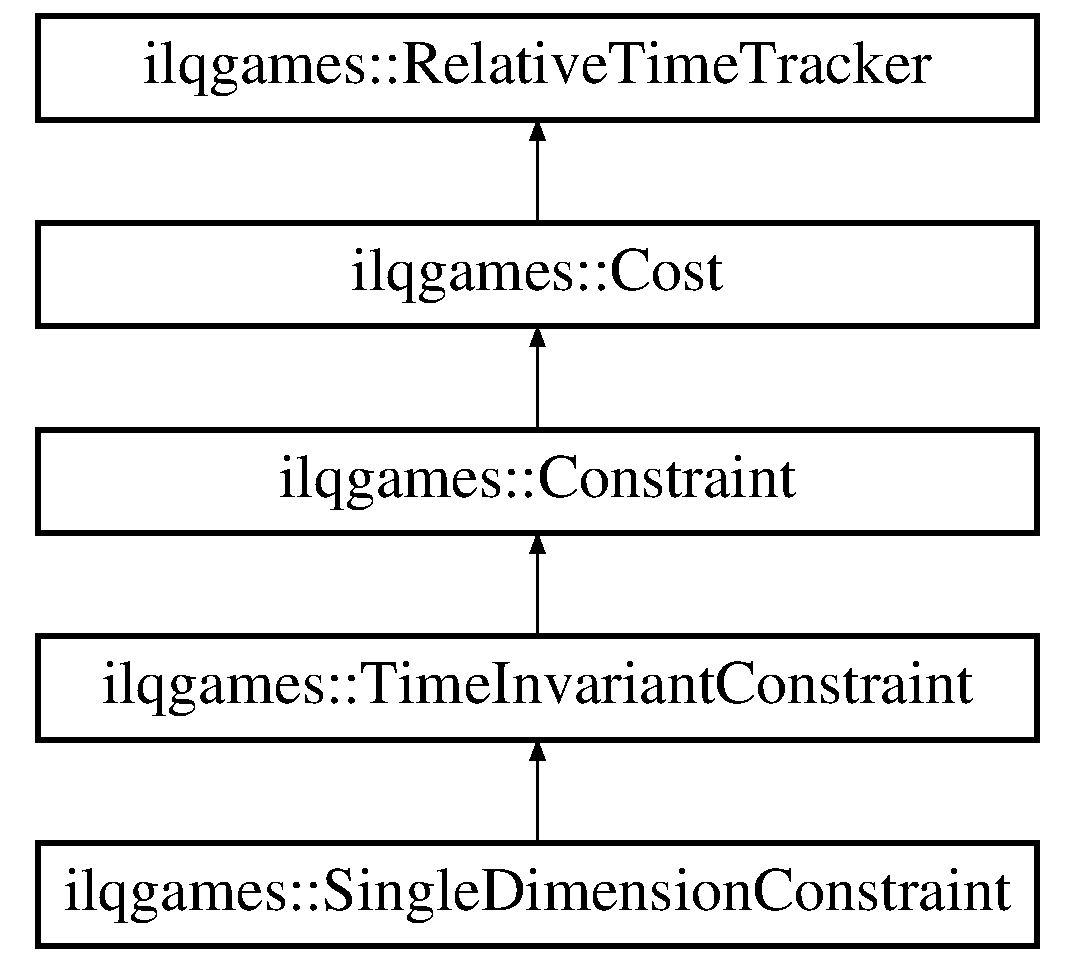
\includegraphics[height=4.000000cm]{classilqgames_1_1_single_dimension_constraint}
\end{center}
\end{figure}
\subsection*{Public Member Functions}
\begin{DoxyCompactItemize}
\item 
{\bfseries Single\+Dimension\+Constraint} (Dimension dimension, float threshold, bool oriented\+\_\+right, const std\+::string \&name=\char`\"{}\char`\"{})\hypertarget{classilqgames_1_1_single_dimension_constraint_ac9f91e5938602c15b23b48756866b84e}{}\label{classilqgames_1_1_single_dimension_constraint_ac9f91e5938602c15b23b48756866b84e}

\item 
bool {\bfseries Is\+Satisfied} (const Vector\+Xf \&input, float $\ast$level=nullptr) const \hypertarget{classilqgames_1_1_single_dimension_constraint_a17cf10a6380cd6bf93523e3da37b1701}{}\label{classilqgames_1_1_single_dimension_constraint_a17cf10a6380cd6bf93523e3da37b1701}

\item 
void {\bfseries Quadraticize} (const Vector\+Xf \&input, Matrix\+Xf $\ast$hess, Vector\+Xf $\ast$grad) const \hypertarget{classilqgames_1_1_single_dimension_constraint_a4079f6f9af8858c0520d60133a5ef3fb}{}\label{classilqgames_1_1_single_dimension_constraint_a4079f6f9af8858c0520d60133a5ef3fb}

\end{DoxyCompactItemize}
\subsection*{Additional Inherited Members}


\subsection{Detailed Description}


Definition at line 56 of file single\+\_\+dimension\+\_\+constraint.\+h.



The documentation for this class was generated from the following files\+:\begin{DoxyCompactItemize}
\item 
/home/travis/build/\+H\+J\+Reachability/ilqgames/include/ilqgames/constraint/single\+\_\+dimension\+\_\+constraint.\+h\item 
/home/travis/build/\+H\+J\+Reachability/ilqgames/src/single\+\_\+dimension\+\_\+constraint.\+cpp\end{DoxyCompactItemize}

\hypertarget{classilqgames_1_1_single_player_car5_d}{}\section{ilqgames\+:\+:Single\+Player\+Car5D Class Reference}
\label{classilqgames_1_1_single_player_car5_d}\index{ilqgames\+::\+Single\+Player\+Car5D@{ilqgames\+::\+Single\+Player\+Car5D}}
Inheritance diagram for ilqgames\+:\+:Single\+Player\+Car5D\+:\begin{figure}[H]
\begin{center}
\leavevmode
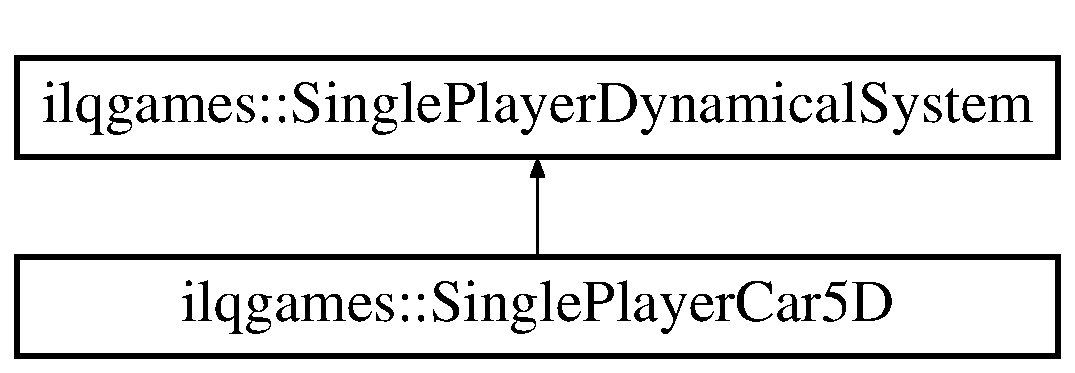
\includegraphics[height=2.000000cm]{classilqgames_1_1_single_player_car5_d}
\end{center}
\end{figure}
\subsection*{Public Member Functions}
\begin{DoxyCompactItemize}
\item 
{\bfseries Single\+Player\+Car5D} (float inter\+\_\+axle\+\_\+distance)\hypertarget{classilqgames_1_1_single_player_car5_d_aa2d4167f0643ec567c9b972027ef4097}{}\label{classilqgames_1_1_single_player_car5_d_aa2d4167f0643ec567c9b972027ef4097}

\item 
Vector\+Xf {\bfseries Evaluate} (Time t, const Vector\+Xf \&x, const Vector\+Xf \&u) const \hypertarget{classilqgames_1_1_single_player_car5_d_aec8946c18a72299e3b6fd01cb7eda35b}{}\label{classilqgames_1_1_single_player_car5_d_aec8946c18a72299e3b6fd01cb7eda35b}

\item 
void {\bfseries Linearize} (Time t, Time time\+\_\+step, const Vector\+Xf \&x, const Vector\+Xf \&u, Eigen\+::\+Ref$<$ Matrix\+Xf $>$ A, Eigen\+::\+Ref$<$ Matrix\+Xf $>$ B) const \hypertarget{classilqgames_1_1_single_player_car5_d_a9059f7965c8909944968d5445aee26b4}{}\label{classilqgames_1_1_single_player_car5_d_a9059f7965c8909944968d5445aee26b4}

\item 
float {\bfseries Distance\+Between} (const Vector\+Xf \&x0, const Vector\+Xf \&x1) const \hypertarget{classilqgames_1_1_single_player_car5_d_a1926a9e26bbca135158bf6e2f30c0fff}{}\label{classilqgames_1_1_single_player_car5_d_a1926a9e26bbca135158bf6e2f30c0fff}

\item 
std\+::vector$<$ Dimension $>$ {\bfseries Position\+Dimensions} () const \hypertarget{classilqgames_1_1_single_player_car5_d_aeb5fabf794950ec8e55e37d685c20027}{}\label{classilqgames_1_1_single_player_car5_d_aeb5fabf794950ec8e55e37d685c20027}

\end{DoxyCompactItemize}
\subsection*{Static Public Attributes}
\begin{DoxyCompactItemize}
\item 
static const Dimension {\bfseries k\+Num\+X\+Dims} = 5\hypertarget{classilqgames_1_1_single_player_car5_d_ae04424bf5f58c4ac50d930463de7651e}{}\label{classilqgames_1_1_single_player_car5_d_ae04424bf5f58c4ac50d930463de7651e}

\item 
static const Dimension {\bfseries k\+Px\+Idx} = 0\hypertarget{classilqgames_1_1_single_player_car5_d_af631fa1ae88fccb70c162f5d53bbc7d1}{}\label{classilqgames_1_1_single_player_car5_d_af631fa1ae88fccb70c162f5d53bbc7d1}

\item 
static const Dimension {\bfseries k\+Py\+Idx} = 1\hypertarget{classilqgames_1_1_single_player_car5_d_a89bcf731951ba546415bc3fce0cb6610}{}\label{classilqgames_1_1_single_player_car5_d_a89bcf731951ba546415bc3fce0cb6610}

\item 
static const Dimension {\bfseries k\+Theta\+Idx} = 2\hypertarget{classilqgames_1_1_single_player_car5_d_ac8a6c8c70cb00fc92a2d55aaebb64e30}{}\label{classilqgames_1_1_single_player_car5_d_ac8a6c8c70cb00fc92a2d55aaebb64e30}

\item 
static const Dimension {\bfseries k\+Phi\+Idx} = 3\hypertarget{classilqgames_1_1_single_player_car5_d_acfb3ccd7eacfe1940d8701a9f0e377a9}{}\label{classilqgames_1_1_single_player_car5_d_acfb3ccd7eacfe1940d8701a9f0e377a9}

\item 
static const Dimension {\bfseries k\+V\+Idx} = 4\hypertarget{classilqgames_1_1_single_player_car5_d_add1a5eda6959262886b179f563e86220}{}\label{classilqgames_1_1_single_player_car5_d_add1a5eda6959262886b179f563e86220}

\item 
static const Dimension {\bfseries k\+Num\+U\+Dims} = 2\hypertarget{classilqgames_1_1_single_player_car5_d_a1ec05771f187067850d48008c4ddd177}{}\label{classilqgames_1_1_single_player_car5_d_a1ec05771f187067850d48008c4ddd177}

\item 
static const Dimension {\bfseries k\+Omega\+Idx} = 0\hypertarget{classilqgames_1_1_single_player_car5_d_a631c9ad5ab268bb1b4e1c9e47b0ecfea}{}\label{classilqgames_1_1_single_player_car5_d_a631c9ad5ab268bb1b4e1c9e47b0ecfea}

\item 
static const Dimension {\bfseries k\+A\+Idx} = 1\hypertarget{classilqgames_1_1_single_player_car5_d_afa3f09428338b06f881a540a8fa9dd06}{}\label{classilqgames_1_1_single_player_car5_d_afa3f09428338b06f881a540a8fa9dd06}

\end{DoxyCompactItemize}
\subsection*{Additional Inherited Members}


\subsection{Detailed Description}


Definition at line 60 of file single\+\_\+player\+\_\+car\+\_\+5d.\+h.



The documentation for this class was generated from the following files\+:\begin{DoxyCompactItemize}
\item 
/home/travis/build/\+H\+J\+Reachability/ilqgames/include/ilqgames/dynamics/single\+\_\+player\+\_\+car\+\_\+5d.\+h\item 
/home/travis/build/\+H\+J\+Reachability/ilqgames/src/single\+\_\+player\+\_\+car\+\_\+5d.\+cpp\end{DoxyCompactItemize}

\hypertarget{classilqgames_1_1_single_player_car6_d}{}\section{ilqgames\+:\+:Single\+Player\+Car6D Class Reference}
\label{classilqgames_1_1_single_player_car6_d}\index{ilqgames\+::\+Single\+Player\+Car6D@{ilqgames\+::\+Single\+Player\+Car6D}}
Inheritance diagram for ilqgames\+:\+:Single\+Player\+Car6D\+:\begin{figure}[H]
\begin{center}
\leavevmode
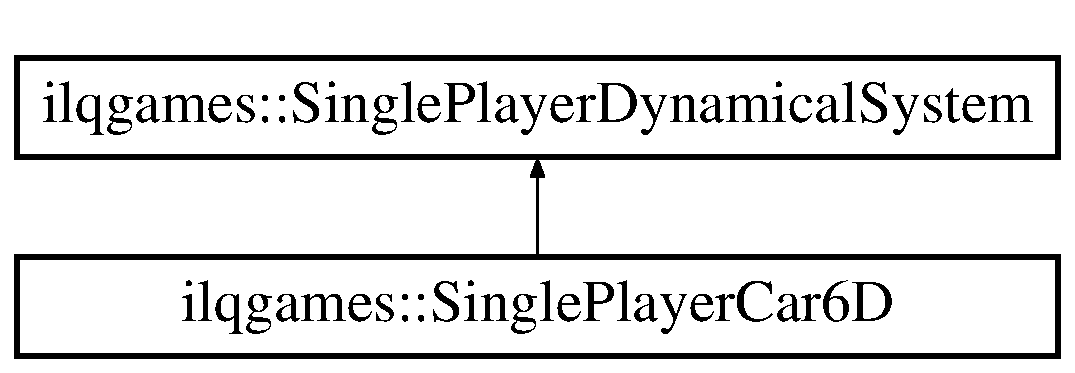
\includegraphics[height=2.000000cm]{classilqgames_1_1_single_player_car6_d}
\end{center}
\end{figure}
\subsection*{Public Member Functions}
\begin{DoxyCompactItemize}
\item 
{\bfseries Single\+Player\+Car6D} (float inter\+\_\+axle\+\_\+distance)\hypertarget{classilqgames_1_1_single_player_car6_d_a1447d0191222caa085c9136e776b75a2}{}\label{classilqgames_1_1_single_player_car6_d_a1447d0191222caa085c9136e776b75a2}

\item 
Vector\+Xf {\bfseries Evaluate} (Time t, const Vector\+Xf \&x, const Vector\+Xf \&u) const \hypertarget{classilqgames_1_1_single_player_car6_d_a60e07c8bde8c99b24f674b78b61c1f82}{}\label{classilqgames_1_1_single_player_car6_d_a60e07c8bde8c99b24f674b78b61c1f82}

\item 
void {\bfseries Linearize} (Time t, const Vector\+Xf \&x, const Vector\+Xf \&u, Eigen\+::\+Ref$<$ Matrix\+Xf $>$ A, Eigen\+::\+Ref$<$ Matrix\+Xf $>$ B) const \hypertarget{classilqgames_1_1_single_player_car6_d_ab0c9fb5d14a4545db7692a54e5320007}{}\label{classilqgames_1_1_single_player_car6_d_ab0c9fb5d14a4545db7692a54e5320007}

\item 
float {\bfseries Distance\+Between} (const Vector\+Xf \&x0, const Vector\+Xf \&x1) const \hypertarget{classilqgames_1_1_single_player_car6_d_a4874842c55f3591e26707e1440466ff6}{}\label{classilqgames_1_1_single_player_car6_d_a4874842c55f3591e26707e1440466ff6}

\item 
std\+::vector$<$ Dimension $>$ {\bfseries Position\+Dimensions} () const \hypertarget{classilqgames_1_1_single_player_car6_d_abd33eafcc1243df1bac72006fc8fd0f5}{}\label{classilqgames_1_1_single_player_car6_d_abd33eafcc1243df1bac72006fc8fd0f5}

\end{DoxyCompactItemize}
\subsection*{Static Public Attributes}
\begin{DoxyCompactItemize}
\item 
static const Dimension {\bfseries k\+Num\+X\+Dims} = 6\hypertarget{classilqgames_1_1_single_player_car6_d_ab65826aa1e17810e7e84d4a0aa65938c}{}\label{classilqgames_1_1_single_player_car6_d_ab65826aa1e17810e7e84d4a0aa65938c}

\item 
static const Dimension {\bfseries k\+Px\+Idx} = 0\hypertarget{classilqgames_1_1_single_player_car6_d_ab825013346aa8aa9974dd7f5cc676381}{}\label{classilqgames_1_1_single_player_car6_d_ab825013346aa8aa9974dd7f5cc676381}

\item 
static const Dimension {\bfseries k\+Py\+Idx} = 1\hypertarget{classilqgames_1_1_single_player_car6_d_aa372e45ff22be1c2b05d7f20c8e383a7}{}\label{classilqgames_1_1_single_player_car6_d_aa372e45ff22be1c2b05d7f20c8e383a7}

\item 
static const Dimension {\bfseries k\+Theta\+Idx} = 2\hypertarget{classilqgames_1_1_single_player_car6_d_a2abea98223a93c58c29faad32ac38255}{}\label{classilqgames_1_1_single_player_car6_d_a2abea98223a93c58c29faad32ac38255}

\item 
static const Dimension {\bfseries k\+Phi\+Idx} = 3\hypertarget{classilqgames_1_1_single_player_car6_d_a4c771b9f2bde8507ef3579b476650e33}{}\label{classilqgames_1_1_single_player_car6_d_a4c771b9f2bde8507ef3579b476650e33}

\item 
static const Dimension {\bfseries k\+V\+Idx} = 4\hypertarget{classilqgames_1_1_single_player_car6_d_aa34edbf40b6d9de9339a3e4bc33bb830}{}\label{classilqgames_1_1_single_player_car6_d_aa34edbf40b6d9de9339a3e4bc33bb830}

\item 
static const Dimension {\bfseries k\+A\+Idx} = 5\hypertarget{classilqgames_1_1_single_player_car6_d_a7ae828d7bb2d60516a7c3671edcbffac}{}\label{classilqgames_1_1_single_player_car6_d_a7ae828d7bb2d60516a7c3671edcbffac}

\item 
static const Dimension {\bfseries k\+Num\+U\+Dims} = 2\hypertarget{classilqgames_1_1_single_player_car6_d_a45cfff4d14fa369911175ee0b90b5511}{}\label{classilqgames_1_1_single_player_car6_d_a45cfff4d14fa369911175ee0b90b5511}

\item 
static const Dimension {\bfseries k\+Omega\+Idx} = 0\hypertarget{classilqgames_1_1_single_player_car6_d_af76abcc4941bee9a03a2a48f02549682}{}\label{classilqgames_1_1_single_player_car6_d_af76abcc4941bee9a03a2a48f02549682}

\item 
static const Dimension {\bfseries k\+Jerk\+Idx} = 1\hypertarget{classilqgames_1_1_single_player_car6_d_a619427a67ea75bbba027a90f00a8cede}{}\label{classilqgames_1_1_single_player_car6_d_a619427a67ea75bbba027a90f00a8cede}

\end{DoxyCompactItemize}
\subsection*{Additional Inherited Members}


\subsection{Detailed Description}


Definition at line 61 of file single\+\_\+player\+\_\+car\+\_\+6d.\+h.



The documentation for this class was generated from the following files\+:\begin{DoxyCompactItemize}
\item 
/home/travis/build/\+H\+J\+Reachability/ilqgames/include/ilqgames/dynamics/single\+\_\+player\+\_\+car\+\_\+6d.\+h\item 
/home/travis/build/\+H\+J\+Reachability/ilqgames/src/single\+\_\+player\+\_\+car\+\_\+6d.\+cpp\end{DoxyCompactItemize}

\hypertarget{classilqgames_1_1_single_player_car7_d}{}\section{ilqgames\+:\+:Single\+Player\+Car7D Class Reference}
\label{classilqgames_1_1_single_player_car7_d}\index{ilqgames\+::\+Single\+Player\+Car7D@{ilqgames\+::\+Single\+Player\+Car7D}}
Inheritance diagram for ilqgames\+:\+:Single\+Player\+Car7D\+:\begin{figure}[H]
\begin{center}
\leavevmode
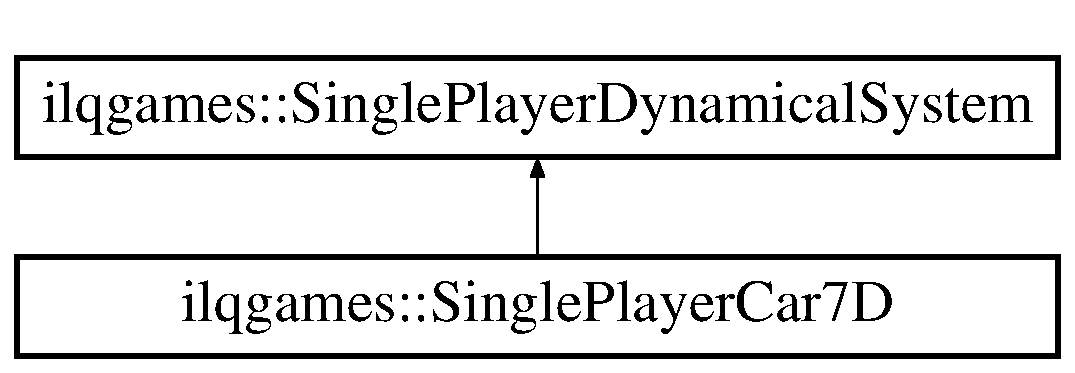
\includegraphics[height=2.000000cm]{classilqgames_1_1_single_player_car7_d}
\end{center}
\end{figure}
\subsection*{Public Member Functions}
\begin{DoxyCompactItemize}
\item 
{\bfseries Single\+Player\+Car7D} (float inter\+\_\+axle\+\_\+distance)\hypertarget{classilqgames_1_1_single_player_car7_d_a31ca08f1230c5c180d8b1f55230f4c49}{}\label{classilqgames_1_1_single_player_car7_d_a31ca08f1230c5c180d8b1f55230f4c49}

\item 
Vector\+Xf {\bfseries Evaluate} (Time t, const Vector\+Xf \&x, const Vector\+Xf \&u) const \hypertarget{classilqgames_1_1_single_player_car7_d_a84d452cb5dd31f143d75def83a14f4c3}{}\label{classilqgames_1_1_single_player_car7_d_a84d452cb5dd31f143d75def83a14f4c3}

\item 
void {\bfseries Linearize} (Time t, Time time\+\_\+step, const Vector\+Xf \&x, const Vector\+Xf \&u, Eigen\+::\+Ref$<$ Matrix\+Xf $>$ A, Eigen\+::\+Ref$<$ Matrix\+Xf $>$ B) const \hypertarget{classilqgames_1_1_single_player_car7_d_a206924124fe73eefa173f4e9c52a1c6d}{}\label{classilqgames_1_1_single_player_car7_d_a206924124fe73eefa173f4e9c52a1c6d}

\item 
float {\bfseries Distance\+Between} (const Vector\+Xf \&x0, const Vector\+Xf \&x1) const \hypertarget{classilqgames_1_1_single_player_car7_d_a409dce5e2bb27fabd19057fb5084187f}{}\label{classilqgames_1_1_single_player_car7_d_a409dce5e2bb27fabd19057fb5084187f}

\end{DoxyCompactItemize}
\subsection*{Static Public Attributes}
\begin{DoxyCompactItemize}
\item 
static const Dimension {\bfseries k\+Num\+X\+Dims} = 7\hypertarget{classilqgames_1_1_single_player_car7_d_a1f847cd0b3ddd30ff4bc3c8d862bdfe4}{}\label{classilqgames_1_1_single_player_car7_d_a1f847cd0b3ddd30ff4bc3c8d862bdfe4}

\item 
static const Dimension {\bfseries k\+Px\+Idx} = 0\hypertarget{classilqgames_1_1_single_player_car7_d_aa5aa5a86d38a9e27bf11b7b388fbd5c5}{}\label{classilqgames_1_1_single_player_car7_d_aa5aa5a86d38a9e27bf11b7b388fbd5c5}

\item 
static const Dimension {\bfseries k\+Py\+Idx} = 1\hypertarget{classilqgames_1_1_single_player_car7_d_aa845e784cdd13b3195b9c3d32496980e}{}\label{classilqgames_1_1_single_player_car7_d_aa845e784cdd13b3195b9c3d32496980e}

\item 
static const Dimension {\bfseries k\+Theta\+Idx} = 2\hypertarget{classilqgames_1_1_single_player_car7_d_a95a8d6508be2af252e337a3474c6b215}{}\label{classilqgames_1_1_single_player_car7_d_a95a8d6508be2af252e337a3474c6b215}

\item 
static const Dimension {\bfseries k\+Phi\+Idx} = 3\hypertarget{classilqgames_1_1_single_player_car7_d_a8ed59f5a4f1c39b5d7695c6fe44ecf50}{}\label{classilqgames_1_1_single_player_car7_d_a8ed59f5a4f1c39b5d7695c6fe44ecf50}

\item 
static const Dimension {\bfseries k\+V\+Idx} = 4\hypertarget{classilqgames_1_1_single_player_car7_d_aa0f9cc445052fcca2e233cf6f9d50070}{}\label{classilqgames_1_1_single_player_car7_d_aa0f9cc445052fcca2e233cf6f9d50070}

\item 
static const Dimension {\bfseries k\+Kappa\+Idx} = 5\hypertarget{classilqgames_1_1_single_player_car7_d_aca71669442d0e7b2a57b87e11c5ec438}{}\label{classilqgames_1_1_single_player_car7_d_aca71669442d0e7b2a57b87e11c5ec438}

\item 
static const Dimension {\bfseries k\+S\+Idx} = 6\hypertarget{classilqgames_1_1_single_player_car7_d_a593134a90cf4e3ac7ec105b6774e66c1}{}\label{classilqgames_1_1_single_player_car7_d_a593134a90cf4e3ac7ec105b6774e66c1}

\item 
static const Dimension {\bfseries k\+Num\+U\+Dims} = 2\hypertarget{classilqgames_1_1_single_player_car7_d_a82513dac7d45b3881512cf06b8abda84}{}\label{classilqgames_1_1_single_player_car7_d_a82513dac7d45b3881512cf06b8abda84}

\item 
static const Dimension {\bfseries k\+Omega\+Idx} = 0\hypertarget{classilqgames_1_1_single_player_car7_d_a0a795d59a3fd1e741ebc6c5bbc092ac9}{}\label{classilqgames_1_1_single_player_car7_d_a0a795d59a3fd1e741ebc6c5bbc092ac9}

\item 
static const Dimension {\bfseries k\+A\+Idx} = 1\hypertarget{classilqgames_1_1_single_player_car7_d_a93cc9c23a5f4c18ddd397a5fe29060af}{}\label{classilqgames_1_1_single_player_car7_d_a93cc9c23a5f4c18ddd397a5fe29060af}

\end{DoxyCompactItemize}
\subsection*{Additional Inherited Members}


\subsection{Detailed Description}


Definition at line 63 of file single\+\_\+player\+\_\+car\+\_\+7d.\+h.



The documentation for this class was generated from the following files\+:\begin{DoxyCompactItemize}
\item 
/home/travis/build/\+H\+J\+Reachability/ilqgames/include/ilqgames/dynamics/single\+\_\+player\+\_\+car\+\_\+7d.\+h\item 
/home/travis/build/\+H\+J\+Reachability/ilqgames/src/single\+\_\+player\+\_\+car\+\_\+7d.\+cpp\end{DoxyCompactItemize}

\hypertarget{classilqgames_1_1_single_player_delayed_dubins_car}{}\section{ilqgames\+:\+:Single\+Player\+Delayed\+Dubins\+Car Class Reference}
\label{classilqgames_1_1_single_player_delayed_dubins_car}\index{ilqgames\+::\+Single\+Player\+Delayed\+Dubins\+Car@{ilqgames\+::\+Single\+Player\+Delayed\+Dubins\+Car}}
Inheritance diagram for ilqgames\+:\+:Single\+Player\+Delayed\+Dubins\+Car\+:\begin{figure}[H]
\begin{center}
\leavevmode
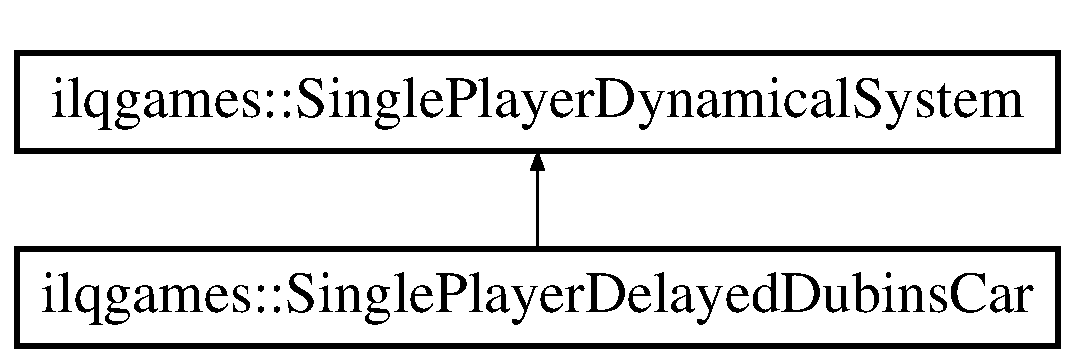
\includegraphics[height=2.000000cm]{classilqgames_1_1_single_player_delayed_dubins_car}
\end{center}
\end{figure}
\subsection*{Public Member Functions}
\begin{DoxyCompactItemize}
\item 
{\bfseries Single\+Player\+Delayed\+Dubins\+Car} (float v)\hypertarget{classilqgames_1_1_single_player_delayed_dubins_car_aa6ba6ca3a5e0b6c80d9199e2c12ced47}{}\label{classilqgames_1_1_single_player_delayed_dubins_car_aa6ba6ca3a5e0b6c80d9199e2c12ced47}

\item 
Vector\+Xf {\bfseries Evaluate} (Time t, const Vector\+Xf \&x, const Vector\+Xf \&u) const \hypertarget{classilqgames_1_1_single_player_delayed_dubins_car_a6540f0ba900dfd2e49e920a066646a39}{}\label{classilqgames_1_1_single_player_delayed_dubins_car_a6540f0ba900dfd2e49e920a066646a39}

\item 
void {\bfseries Linearize} (Time t, const Vector\+Xf \&x, const Vector\+Xf \&u, Eigen\+::\+Ref$<$ Matrix\+Xf $>$ A, Eigen\+::\+Ref$<$ Matrix\+Xf $>$ B) const \hypertarget{classilqgames_1_1_single_player_delayed_dubins_car_a312c7025e8cdfb8baf7bc448c96d2047}{}\label{classilqgames_1_1_single_player_delayed_dubins_car_a312c7025e8cdfb8baf7bc448c96d2047}

\item 
std\+::vector$<$ Dimension $>$ {\bfseries Position\+Dimensions} () const \hypertarget{classilqgames_1_1_single_player_delayed_dubins_car_aa6e368f3b2235bda5adbe5b0e5337c2e}{}\label{classilqgames_1_1_single_player_delayed_dubins_car_aa6e368f3b2235bda5adbe5b0e5337c2e}

\end{DoxyCompactItemize}
\subsection*{Static Public Attributes}
\begin{DoxyCompactItemize}
\item 
static const Dimension {\bfseries k\+Num\+X\+Dims} = 4\hypertarget{classilqgames_1_1_single_player_delayed_dubins_car_acc716afb8d6612fa8096fa22704344a9}{}\label{classilqgames_1_1_single_player_delayed_dubins_car_acc716afb8d6612fa8096fa22704344a9}

\item 
static const Dimension {\bfseries k\+Px\+Idx} = 0\hypertarget{classilqgames_1_1_single_player_delayed_dubins_car_a3b3c8adfc51dd087e3215a651fb89c24}{}\label{classilqgames_1_1_single_player_delayed_dubins_car_a3b3c8adfc51dd087e3215a651fb89c24}

\item 
static const Dimension {\bfseries k\+Py\+Idx} = 1\hypertarget{classilqgames_1_1_single_player_delayed_dubins_car_a7291db6867fbb9b1a196d5867a80b296}{}\label{classilqgames_1_1_single_player_delayed_dubins_car_a7291db6867fbb9b1a196d5867a80b296}

\item 
static const Dimension {\bfseries k\+Theta\+Idx} = 2\hypertarget{classilqgames_1_1_single_player_delayed_dubins_car_a87bd0d8387583200c69f0fe9be22f07c}{}\label{classilqgames_1_1_single_player_delayed_dubins_car_a87bd0d8387583200c69f0fe9be22f07c}

\item 
static const Dimension {\bfseries k\+Omega\+Idx} = 3\hypertarget{classilqgames_1_1_single_player_delayed_dubins_car_aafea6f56b9f6797b8ec35c1a3413ac60}{}\label{classilqgames_1_1_single_player_delayed_dubins_car_aafea6f56b9f6797b8ec35c1a3413ac60}

\item 
static const Dimension {\bfseries k\+Num\+U\+Dims} = 1\hypertarget{classilqgames_1_1_single_player_delayed_dubins_car_af9e824e416779d95c089ab751112b713}{}\label{classilqgames_1_1_single_player_delayed_dubins_car_af9e824e416779d95c089ab751112b713}

\item 
static const Dimension {\bfseries k\+Alpha\+Idx} = 0\hypertarget{classilqgames_1_1_single_player_delayed_dubins_car_a7702cfc6fb5d78abdfe99ed549482998}{}\label{classilqgames_1_1_single_player_delayed_dubins_car_a7702cfc6fb5d78abdfe99ed549482998}

\end{DoxyCompactItemize}
\subsection*{Additional Inherited Members}


\subsection{Detailed Description}


Definition at line 59 of file single\+\_\+player\+\_\+delayed\+\_\+dubins\+\_\+car.\+h.



The documentation for this class was generated from the following files\+:\begin{DoxyCompactItemize}
\item 
/home/travis/build/\+H\+J\+Reachability/ilqgames/include/ilqgames/dynamics/single\+\_\+player\+\_\+delayed\+\_\+dubins\+\_\+car.\+h\item 
/home/travis/build/\+H\+J\+Reachability/ilqgames/src/single\+\_\+player\+\_\+delayed\+\_\+dubins\+\_\+car.\+cpp\end{DoxyCompactItemize}

\hypertarget{classilqgames_1_1_single_player_dubins_car}{}\section{ilqgames\+:\+:Single\+Player\+Dubins\+Car Class Reference}
\label{classilqgames_1_1_single_player_dubins_car}\index{ilqgames\+::\+Single\+Player\+Dubins\+Car@{ilqgames\+::\+Single\+Player\+Dubins\+Car}}
Inheritance diagram for ilqgames\+:\+:Single\+Player\+Dubins\+Car\+:\begin{figure}[H]
\begin{center}
\leavevmode
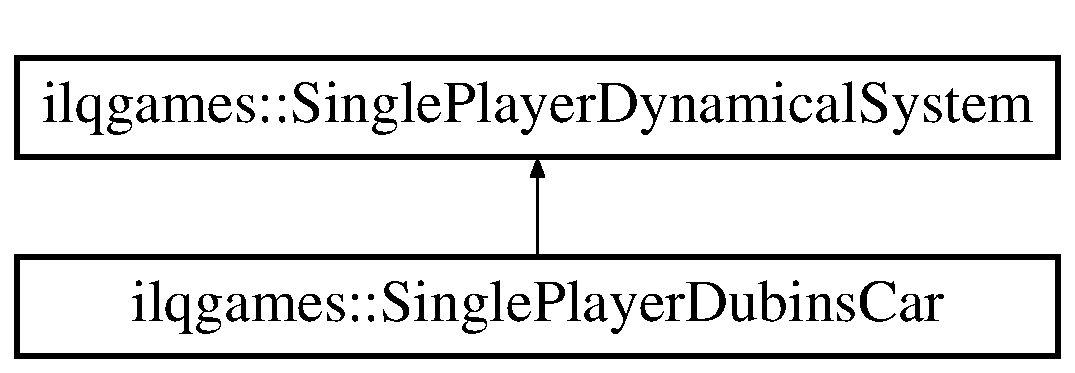
\includegraphics[height=2.000000cm]{classilqgames_1_1_single_player_dubins_car}
\end{center}
\end{figure}
\subsection*{Public Member Functions}
\begin{DoxyCompactItemize}
\item 
{\bfseries Single\+Player\+Dubins\+Car} (float v)\hypertarget{classilqgames_1_1_single_player_dubins_car_aa035123822485f51501c6f0f21a59c34}{}\label{classilqgames_1_1_single_player_dubins_car_aa035123822485f51501c6f0f21a59c34}

\item 
Vector\+Xf {\bfseries Evaluate} (Time t, const Vector\+Xf \&x, const Vector\+Xf \&u) const \hypertarget{classilqgames_1_1_single_player_dubins_car_a8f44090ac61f4543043fd9351b9192bb}{}\label{classilqgames_1_1_single_player_dubins_car_a8f44090ac61f4543043fd9351b9192bb}

\item 
void {\bfseries Linearize} (Time t, Time time\+\_\+step, const Vector\+Xf \&x, const Vector\+Xf \&u, Eigen\+::\+Ref$<$ Matrix\+Xf $>$ A, Eigen\+::\+Ref$<$ Matrix\+Xf $>$ B) const \hypertarget{classilqgames_1_1_single_player_dubins_car_a24b3cd9d9d9764099b48f216a8133214}{}\label{classilqgames_1_1_single_player_dubins_car_a24b3cd9d9d9764099b48f216a8133214}

\end{DoxyCompactItemize}
\subsection*{Static Public Attributes}
\begin{DoxyCompactItemize}
\item 
static const Dimension {\bfseries k\+Num\+X\+Dims} = 3\hypertarget{classilqgames_1_1_single_player_dubins_car_a8c5f6a8a06b4bdefbd9a56c7a5bbd193}{}\label{classilqgames_1_1_single_player_dubins_car_a8c5f6a8a06b4bdefbd9a56c7a5bbd193}

\item 
static const Dimension {\bfseries k\+Px\+Idx} = 0\hypertarget{classilqgames_1_1_single_player_dubins_car_aa804a3752e51f8bb5b72fd9aeb8be36f}{}\label{classilqgames_1_1_single_player_dubins_car_aa804a3752e51f8bb5b72fd9aeb8be36f}

\item 
static const Dimension {\bfseries k\+Py\+Idx} = 1\hypertarget{classilqgames_1_1_single_player_dubins_car_aa1d26063db82735de0b9cace00b7b53a}{}\label{classilqgames_1_1_single_player_dubins_car_aa1d26063db82735de0b9cace00b7b53a}

\item 
static const Dimension {\bfseries k\+Theta\+Idx} = 2\hypertarget{classilqgames_1_1_single_player_dubins_car_a4a7244d2b430f62e6c993e01a0a54a44}{}\label{classilqgames_1_1_single_player_dubins_car_a4a7244d2b430f62e6c993e01a0a54a44}

\item 
static const Dimension {\bfseries k\+Num\+U\+Dims} = 1\hypertarget{classilqgames_1_1_single_player_dubins_car_a2751da81d773417cb83d66ade7f55224}{}\label{classilqgames_1_1_single_player_dubins_car_a2751da81d773417cb83d66ade7f55224}

\item 
static const Dimension {\bfseries k\+Omega\+Idx} = 0\hypertarget{classilqgames_1_1_single_player_dubins_car_aa25171fab5c33ce524c67bf891916dde}{}\label{classilqgames_1_1_single_player_dubins_car_aa25171fab5c33ce524c67bf891916dde}

\end{DoxyCompactItemize}
\subsection*{Additional Inherited Members}


\subsection{Detailed Description}


Definition at line 58 of file single\+\_\+player\+\_\+dubins\+\_\+car.\+h.



The documentation for this class was generated from the following files\+:\begin{DoxyCompactItemize}
\item 
/home/travis/build/\+H\+J\+Reachability/ilqgames/include/ilqgames/dynamics/single\+\_\+player\+\_\+dubins\+\_\+car.\+h\item 
/home/travis/build/\+H\+J\+Reachability/ilqgames/src/single\+\_\+player\+\_\+dubins\+\_\+car.\+cpp\end{DoxyCompactItemize}

\hypertarget{classilqgames_1_1_single_player_dynamical_system}{}\section{ilqgames\+:\+:Single\+Player\+Dynamical\+System Class Reference}
\label{classilqgames_1_1_single_player_dynamical_system}\index{ilqgames\+::\+Single\+Player\+Dynamical\+System@{ilqgames\+::\+Single\+Player\+Dynamical\+System}}
Inheritance diagram for ilqgames\+:\+:Single\+Player\+Dynamical\+System\+:\begin{figure}[H]
\begin{center}
\leavevmode
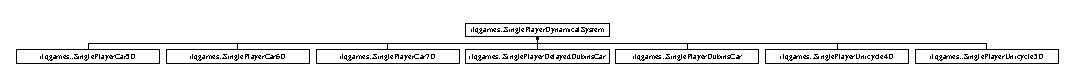
\includegraphics[height=9.000000cm]{classilqgames_1_1_single_player_dynamical_system}
\end{center}
\end{figure}
\subsection*{Public Member Functions}
\begin{DoxyCompactItemize}
\item 
virtual Vector\+Xf {\bfseries Evaluate} (Time t, const Vector\+Xf \&x, const Vector\+Xf \&u) const =0\hypertarget{classilqgames_1_1_single_player_dynamical_system_a6a6fdd6eaf0fd0171d8f87a1648e3320}{}\label{classilqgames_1_1_single_player_dynamical_system_a6a6fdd6eaf0fd0171d8f87a1648e3320}

\item 
virtual void {\bfseries Linearize} (Time t, Time time\+\_\+step, const Vector\+Xf \&x, const Vector\+Xf \&u, Eigen\+::\+Ref$<$ Matrix\+Xf $>$ A, Eigen\+::\+Ref$<$ Matrix\+Xf $>$ B) const =0\hypertarget{classilqgames_1_1_single_player_dynamical_system_a910d13c85415769ba434e6b423390fc9}{}\label{classilqgames_1_1_single_player_dynamical_system_a910d13c85415769ba434e6b423390fc9}

\item 
virtual float {\bfseries Distance\+Between} (const Vector\+Xf \&x0, const Vector\+Xf \&x1) const \hypertarget{classilqgames_1_1_single_player_dynamical_system_a2487c7603c1dc998799c0227d00904f3}{}\label{classilqgames_1_1_single_player_dynamical_system_a2487c7603c1dc998799c0227d00904f3}

\item 
Dimension {\bfseries X\+Dim} () const \hypertarget{classilqgames_1_1_single_player_dynamical_system_a54b50acd4d8eb613c5f1042e38a5f6fd}{}\label{classilqgames_1_1_single_player_dynamical_system_a54b50acd4d8eb613c5f1042e38a5f6fd}

\item 
Dimension {\bfseries U\+Dim} () const \hypertarget{classilqgames_1_1_single_player_dynamical_system_a24d4db1d3ad5450108eb22c412e606c1}{}\label{classilqgames_1_1_single_player_dynamical_system_a24d4db1d3ad5450108eb22c412e606c1}

\item 
virtual std\+::vector$<$ Dimension $>$ {\bfseries Position\+Dimensions} () const =0\hypertarget{classilqgames_1_1_single_player_dynamical_system_add0f6580940de79a76544496ec70d34a}{}\label{classilqgames_1_1_single_player_dynamical_system_add0f6580940de79a76544496ec70d34a}

\end{DoxyCompactItemize}
\subsection*{Protected Member Functions}
\begin{DoxyCompactItemize}
\item 
{\bfseries Single\+Player\+Dynamical\+System} (Dimension xdim, Dimension udim)\hypertarget{classilqgames_1_1_single_player_dynamical_system_aa83761473fdd007d641ff7a29e7c4fe1}{}\label{classilqgames_1_1_single_player_dynamical_system_aa83761473fdd007d641ff7a29e7c4fe1}

\end{DoxyCompactItemize}
\subsection*{Protected Attributes}
\begin{DoxyCompactItemize}
\item 
const Dimension {\bfseries xdim\+\_\+}\hypertarget{classilqgames_1_1_single_player_dynamical_system_a556a93c620d076cf36acd55aff69a02f}{}\label{classilqgames_1_1_single_player_dynamical_system_a556a93c620d076cf36acd55aff69a02f}

\item 
const Dimension {\bfseries udim\+\_\+}\hypertarget{classilqgames_1_1_single_player_dynamical_system_ad7058a359156f603a03323a3abf3de39}{}\label{classilqgames_1_1_single_player_dynamical_system_ad7058a359156f603a03323a3abf3de39}

\end{DoxyCompactItemize}


\subsection{Detailed Description}


Definition at line 51 of file single\+\_\+player\+\_\+dynamical\+\_\+system.\+h.



The documentation for this class was generated from the following file\+:\begin{DoxyCompactItemize}
\item 
/home/travis/build/\+H\+J\+Reachability/ilqgames/include/ilqgames/dynamics/single\+\_\+player\+\_\+dynamical\+\_\+system.\+h\end{DoxyCompactItemize}

\hypertarget{classilqgames_1_1_single_player_flat_car6_d}{}\section{ilqgames\+:\+:Single\+Player\+Flat\+Car6D Class Reference}
\label{classilqgames_1_1_single_player_flat_car6_d}\index{ilqgames\+::\+Single\+Player\+Flat\+Car6D@{ilqgames\+::\+Single\+Player\+Flat\+Car6D}}
Inheritance diagram for ilqgames\+:\+:Single\+Player\+Flat\+Car6D\+:\begin{figure}[H]
\begin{center}
\leavevmode
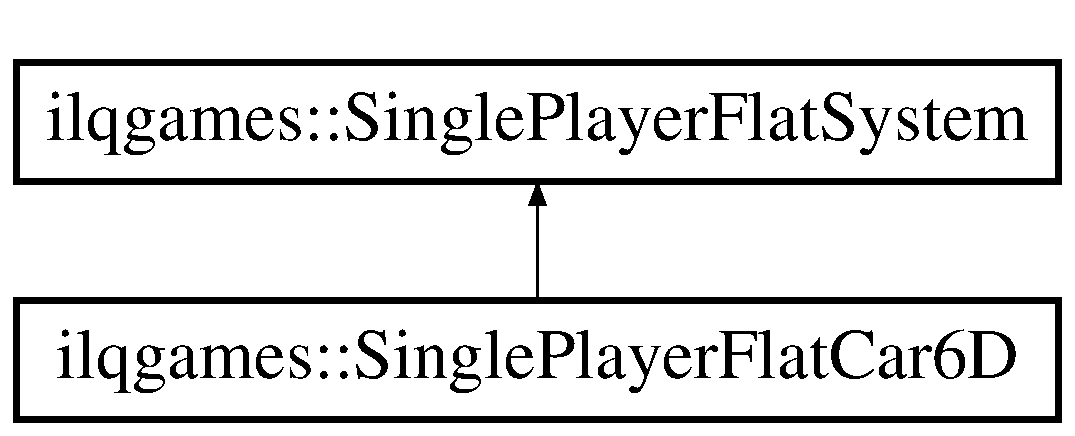
\includegraphics[height=2.000000cm]{classilqgames_1_1_single_player_flat_car6_d}
\end{center}
\end{figure}
\subsection*{Public Member Functions}
\begin{DoxyCompactItemize}
\item 
{\bfseries Single\+Player\+Flat\+Car6D} (float inter\+\_\+axle\+\_\+distance)\hypertarget{classilqgames_1_1_single_player_flat_car6_d_a9fb4fd8e7be90858f22bc536a7bd3222}{}\label{classilqgames_1_1_single_player_flat_car6_d_a9fb4fd8e7be90858f22bc536a7bd3222}

\item 
Vector\+Xf {\bfseries Evaluate} (const Vector\+Xf \&x, const Vector\+Xf \&u) const \hypertarget{classilqgames_1_1_single_player_flat_car6_d_ab1e6af4ef47c00b30ec12420e9691b52}{}\label{classilqgames_1_1_single_player_flat_car6_d_ab1e6af4ef47c00b30ec12420e9691b52}

\item 
void {\bfseries Linearized\+System} (Time time\+\_\+step, Eigen\+::\+Ref$<$ Matrix\+Xf $>$ A, Eigen\+::\+Ref$<$ Matrix\+Xf $>$ B) const \hypertarget{classilqgames_1_1_single_player_flat_car6_d_a2575a1cd3ded4ccd4aea97062a31ba21}{}\label{classilqgames_1_1_single_player_flat_car6_d_a2575a1cd3ded4ccd4aea97062a31ba21}

\item 
Matrix\+Xf {\bfseries Inverse\+Decoupling\+Matrix} (const Vector\+Xf \&x) const \hypertarget{classilqgames_1_1_single_player_flat_car6_d_a236f5a1d6fd3d2d1cb11f4b468efc981}{}\label{classilqgames_1_1_single_player_flat_car6_d_a236f5a1d6fd3d2d1cb11f4b468efc981}

\item 
Vector\+Xf {\bfseries Affine\+Term} (const Vector\+Xf \&x) const \hypertarget{classilqgames_1_1_single_player_flat_car6_d_a662f412d3214b61a99583f2a21647423}{}\label{classilqgames_1_1_single_player_flat_car6_d_a662f412d3214b61a99583f2a21647423}

\item 
Vector\+Xf {\bfseries To\+Linear\+System\+State} (const Vector\+Xf \&x) const \hypertarget{classilqgames_1_1_single_player_flat_car6_d_a514b9407d2e5d7697d366716d11b7d46}{}\label{classilqgames_1_1_single_player_flat_car6_d_a514b9407d2e5d7697d366716d11b7d46}

\item 
Vector\+Xf {\bfseries From\+Linear\+System\+State} (const Vector\+Xf \&xi) const \hypertarget{classilqgames_1_1_single_player_flat_car6_d_a3526acc25cf14c614fdf5b3d8590f269}{}\label{classilqgames_1_1_single_player_flat_car6_d_a3526acc25cf14c614fdf5b3d8590f269}

\item 
void {\bfseries Partial} (const Vector\+Xf \&xi, std\+::vector$<$ Vector\+Xf $>$ $\ast$grads, std\+::vector$<$ Matrix\+Xf $>$ $\ast$hesses) const \hypertarget{classilqgames_1_1_single_player_flat_car6_d_a0b6f26a37091274148c0ff247d13a84b}{}\label{classilqgames_1_1_single_player_flat_car6_d_a0b6f26a37091274148c0ff247d13a84b}

\item 
bool {\bfseries Is\+Linear\+System\+State\+Singular} (const Vector\+Xf \&xi) const \hypertarget{classilqgames_1_1_single_player_flat_car6_d_a7e885c06c72f40ca7a2174cc61850fc3}{}\label{classilqgames_1_1_single_player_flat_car6_d_a7e885c06c72f40ca7a2174cc61850fc3}

\item 
float {\bfseries Distance\+Between} (const Vector\+Xf \&x0, const Vector\+Xf \&x1) const \hypertarget{classilqgames_1_1_single_player_flat_car6_d_afe249fbf6ebdb0449e4d11fd521c10e6}{}\label{classilqgames_1_1_single_player_flat_car6_d_afe249fbf6ebdb0449e4d11fd521c10e6}

\end{DoxyCompactItemize}
\subsection*{Static Public Attributes}
\begin{DoxyCompactItemize}
\item 
static const Dimension {\bfseries k\+Num\+X\+Dims} = 6\hypertarget{classilqgames_1_1_single_player_flat_car6_d_a8f02f15691cbf97bd4b4844d46b2bdf1}{}\label{classilqgames_1_1_single_player_flat_car6_d_a8f02f15691cbf97bd4b4844d46b2bdf1}

\item 
static const Dimension {\bfseries k\+Px\+Idx} = 0\hypertarget{classilqgames_1_1_single_player_flat_car6_d_a553da23880cb7737b5baf536fa137194}{}\label{classilqgames_1_1_single_player_flat_car6_d_a553da23880cb7737b5baf536fa137194}

\item 
static const Dimension {\bfseries k\+Py\+Idx} = 1\hypertarget{classilqgames_1_1_single_player_flat_car6_d_a4676c4f73974f6d74012924856d5de18}{}\label{classilqgames_1_1_single_player_flat_car6_d_a4676c4f73974f6d74012924856d5de18}

\item 
static const Dimension {\bfseries k\+Theta\+Idx} = 2\hypertarget{classilqgames_1_1_single_player_flat_car6_d_aa052602925ac53632106e479566ecb71}{}\label{classilqgames_1_1_single_player_flat_car6_d_aa052602925ac53632106e479566ecb71}

\item 
static const Dimension {\bfseries k\+Phi\+Idx} = 3\hypertarget{classilqgames_1_1_single_player_flat_car6_d_a48dcdb2ec02da3a047b12c5f92d6e05b}{}\label{classilqgames_1_1_single_player_flat_car6_d_a48dcdb2ec02da3a047b12c5f92d6e05b}

\item 
static const Dimension {\bfseries k\+V\+Idx} = 4\hypertarget{classilqgames_1_1_single_player_flat_car6_d_a2c87c3ebe3b7b1fa5f251ff32426e100}{}\label{classilqgames_1_1_single_player_flat_car6_d_a2c87c3ebe3b7b1fa5f251ff32426e100}

\item 
static const Dimension {\bfseries k\+A\+Idx} = 5\hypertarget{classilqgames_1_1_single_player_flat_car6_d_a084b5c8aef49d893ab959a4044fe8c4a}{}\label{classilqgames_1_1_single_player_flat_car6_d_a084b5c8aef49d893ab959a4044fe8c4a}

\item 
static const Dimension {\bfseries k\+Vx\+Idx} = 2\hypertarget{classilqgames_1_1_single_player_flat_car6_d_aa4cad5ddae903c9c507211215e77e8e9}{}\label{classilqgames_1_1_single_player_flat_car6_d_aa4cad5ddae903c9c507211215e77e8e9}

\item 
static const Dimension {\bfseries k\+Vy\+Idx} = 3\hypertarget{classilqgames_1_1_single_player_flat_car6_d_aa20d5310f3056be34cedbb3372fd36a4}{}\label{classilqgames_1_1_single_player_flat_car6_d_aa20d5310f3056be34cedbb3372fd36a4}

\item 
static const Dimension {\bfseries k\+Ax\+Idx} = 4\hypertarget{classilqgames_1_1_single_player_flat_car6_d_a92b405276235bd2f1206a4740660c394}{}\label{classilqgames_1_1_single_player_flat_car6_d_a92b405276235bd2f1206a4740660c394}

\item 
static const Dimension {\bfseries k\+Ay\+Idx} = 5\hypertarget{classilqgames_1_1_single_player_flat_car6_d_a641b93b0a83a4794f8b44f7f387258c1}{}\label{classilqgames_1_1_single_player_flat_car6_d_a641b93b0a83a4794f8b44f7f387258c1}

\item 
static const Dimension {\bfseries k\+Num\+U\+Dims} = 2\hypertarget{classilqgames_1_1_single_player_flat_car6_d_ae8329151026fbee7ed9c59e4a4fd4507}{}\label{classilqgames_1_1_single_player_flat_car6_d_ae8329151026fbee7ed9c59e4a4fd4507}

\item 
static const Dimension {\bfseries k\+Omega\+Idx} = 0\hypertarget{classilqgames_1_1_single_player_flat_car6_d_a9775a4b9e7ee526146b5cfb6631268d8}{}\label{classilqgames_1_1_single_player_flat_car6_d_a9775a4b9e7ee526146b5cfb6631268d8}

\item 
static const Dimension {\bfseries k\+Jerk\+Idx} = 1\hypertarget{classilqgames_1_1_single_player_flat_car6_d_acd36e1fdc5fa7758ef19493cb6766b9c}{}\label{classilqgames_1_1_single_player_flat_car6_d_acd36e1fdc5fa7758ef19493cb6766b9c}

\end{DoxyCompactItemize}
\subsection*{Additional Inherited Members}


\subsection{Detailed Description}


Definition at line 63 of file single\+\_\+player\+\_\+flat\+\_\+car\+\_\+6d.\+h.



The documentation for this class was generated from the following files\+:\begin{DoxyCompactItemize}
\item 
/home/travis/build/\+H\+J\+Reachability/ilqgames/include/ilqgames/dynamics/single\+\_\+player\+\_\+flat\+\_\+car\+\_\+6d.\+h\item 
/home/travis/build/\+H\+J\+Reachability/ilqgames/src/single\+\_\+player\+\_\+flat\+\_\+car\+\_\+6d.\+cpp\end{DoxyCompactItemize}

\hypertarget{classilqgames_1_1_single_player_flat_system}{}\section{ilqgames\+:\+:Single\+Player\+Flat\+System Class Reference}
\label{classilqgames_1_1_single_player_flat_system}\index{ilqgames\+::\+Single\+Player\+Flat\+System@{ilqgames\+::\+Single\+Player\+Flat\+System}}
Inheritance diagram for ilqgames\+:\+:Single\+Player\+Flat\+System\+:\begin{figure}[H]
\begin{center}
\leavevmode
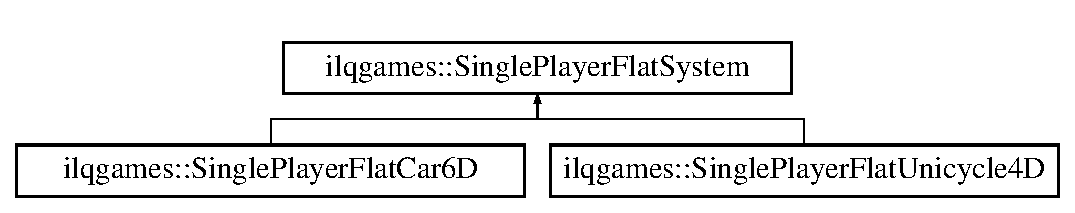
\includegraphics[height=2.000000cm]{classilqgames_1_1_single_player_flat_system}
\end{center}
\end{figure}
\subsection*{Public Member Functions}
\begin{DoxyCompactItemize}
\item 
virtual Vector\+Xf {\bfseries Evaluate} (const Vector\+Xf \&x, const Vector\+Xf \&u) const =0\hypertarget{classilqgames_1_1_single_player_flat_system_a20c9491dcf6871772de086a11d30d5d7}{}\label{classilqgames_1_1_single_player_flat_system_a20c9491dcf6871772de086a11d30d5d7}

\item 
virtual void {\bfseries Linearized\+System} (Eigen\+::\+Ref$<$ Matrix\+Xf $>$ A, Eigen\+::\+Ref$<$ Matrix\+Xf $>$ B) const =0\hypertarget{classilqgames_1_1_single_player_flat_system_a3ee4cb1e9bdcff112bb89875420e88c3}{}\label{classilqgames_1_1_single_player_flat_system_a3ee4cb1e9bdcff112bb89875420e88c3}

\item 
virtual Matrix\+Xf {\bfseries Inverse\+Decoupling\+Matrix} (const Vector\+Xf \&x) const =0\hypertarget{classilqgames_1_1_single_player_flat_system_a3683c7873c019f02d8bfcaa0de1afa16}{}\label{classilqgames_1_1_single_player_flat_system_a3683c7873c019f02d8bfcaa0de1afa16}

\item 
virtual Vector\+Xf {\bfseries Affine\+Term} (const Vector\+Xf \&x) const =0\hypertarget{classilqgames_1_1_single_player_flat_system_a4ce7b06850b71df461800dccf9683a20}{}\label{classilqgames_1_1_single_player_flat_system_a4ce7b06850b71df461800dccf9683a20}

\item 
Vector\+Xf {\bfseries Linearizing\+Control} (const Vector\+Xf \&x, const Vector\+Xf \&v) const \hypertarget{classilqgames_1_1_single_player_flat_system_a4ca811c59babd68b0fdf9d9ed0298431}{}\label{classilqgames_1_1_single_player_flat_system_a4ca811c59babd68b0fdf9d9ed0298431}

\item 
virtual Vector\+Xf {\bfseries To\+Linear\+System\+State} (const Vector\+Xf \&x) const =0\hypertarget{classilqgames_1_1_single_player_flat_system_a594d67986244e731fb70ded660575020}{}\label{classilqgames_1_1_single_player_flat_system_a594d67986244e731fb70ded660575020}

\item 
virtual Vector\+Xf {\bfseries From\+Linear\+System\+State} (const Vector\+Xf \&xi) const =0\hypertarget{classilqgames_1_1_single_player_flat_system_a235d40a141ea4ae6ce39523aa0187d3e}{}\label{classilqgames_1_1_single_player_flat_system_a235d40a141ea4ae6ce39523aa0187d3e}

\item 
virtual bool {\bfseries Is\+Linear\+System\+State\+Singular} (const Vector\+Xf \&xi) const =0\hypertarget{classilqgames_1_1_single_player_flat_system_a7c4f5712a49f29f7e2e5b0bebc645f87}{}\label{classilqgames_1_1_single_player_flat_system_a7c4f5712a49f29f7e2e5b0bebc645f87}

\item 
virtual void {\bfseries Partial} (const Vector\+Xf \&xi, std\+::vector$<$ Vector\+Xf $>$ $\ast$grads, std\+::vector$<$ Matrix\+Xf $>$ $\ast$hesses) const =0\hypertarget{classilqgames_1_1_single_player_flat_system_ac13f3f047b18f757fa0237b79024c22a}{}\label{classilqgames_1_1_single_player_flat_system_ac13f3f047b18f757fa0237b79024c22a}

\item 
virtual float {\bfseries Distance\+Between} (const Vector\+Xf \&x0, const Vector\+Xf \&x1) const \hypertarget{classilqgames_1_1_single_player_flat_system_a887a8c265b40218d02efaf876e6a8843}{}\label{classilqgames_1_1_single_player_flat_system_a887a8c265b40218d02efaf876e6a8843}

\item 
Dimension {\bfseries X\+Dim} () const \hypertarget{classilqgames_1_1_single_player_flat_system_ada9537087ddb5460fed6eff12e6b280b}{}\label{classilqgames_1_1_single_player_flat_system_ada9537087ddb5460fed6eff12e6b280b}

\item 
Dimension {\bfseries U\+Dim} () const \hypertarget{classilqgames_1_1_single_player_flat_system_a47c268e369f91c0b9609af7949c085bb}{}\label{classilqgames_1_1_single_player_flat_system_a47c268e369f91c0b9609af7949c085bb}

\item 
virtual std\+::vector$<$ Dimension $>$ {\bfseries Position\+Dimensions} () const =0\hypertarget{classilqgames_1_1_single_player_flat_system_aab04053f573b24de4332b7e3d6325ec1}{}\label{classilqgames_1_1_single_player_flat_system_aab04053f573b24de4332b7e3d6325ec1}

\end{DoxyCompactItemize}
\subsection*{Protected Member Functions}
\begin{DoxyCompactItemize}
\item 
{\bfseries Single\+Player\+Flat\+System} (Dimension xdim, Dimension udim)\hypertarget{classilqgames_1_1_single_player_flat_system_a4ab18a6147857ce85583ea41c1959a54}{}\label{classilqgames_1_1_single_player_flat_system_a4ab18a6147857ce85583ea41c1959a54}

\end{DoxyCompactItemize}
\subsection*{Protected Attributes}
\begin{DoxyCompactItemize}
\item 
const Dimension {\bfseries xdim\+\_\+}\hypertarget{classilqgames_1_1_single_player_flat_system_aa658a8f808613f170ace84b6aca63a05}{}\label{classilqgames_1_1_single_player_flat_system_aa658a8f808613f170ace84b6aca63a05}

\item 
const Dimension {\bfseries udim\+\_\+}\hypertarget{classilqgames_1_1_single_player_flat_system_a24a3044071823bdd4af74d8d5b89d3d7}{}\label{classilqgames_1_1_single_player_flat_system_a24a3044071823bdd4af74d8d5b89d3d7}

\end{DoxyCompactItemize}


\subsection{Detailed Description}


Definition at line 51 of file single\+\_\+player\+\_\+flat\+\_\+system.\+h.



The documentation for this class was generated from the following file\+:\begin{DoxyCompactItemize}
\item 
/home/travis/build/\+H\+J\+Reachability/ilqgames/include/ilqgames/dynamics/single\+\_\+player\+\_\+flat\+\_\+system.\+h\end{DoxyCompactItemize}

\hypertarget{classilqgames_1_1_single_player_flat_unicycle4_d}{}\section{ilqgames\+:\+:Single\+Player\+Flat\+Unicycle4D Class Reference}
\label{classilqgames_1_1_single_player_flat_unicycle4_d}\index{ilqgames\+::\+Single\+Player\+Flat\+Unicycle4D@{ilqgames\+::\+Single\+Player\+Flat\+Unicycle4D}}
Inheritance diagram for ilqgames\+:\+:Single\+Player\+Flat\+Unicycle4D\+:\begin{figure}[H]
\begin{center}
\leavevmode
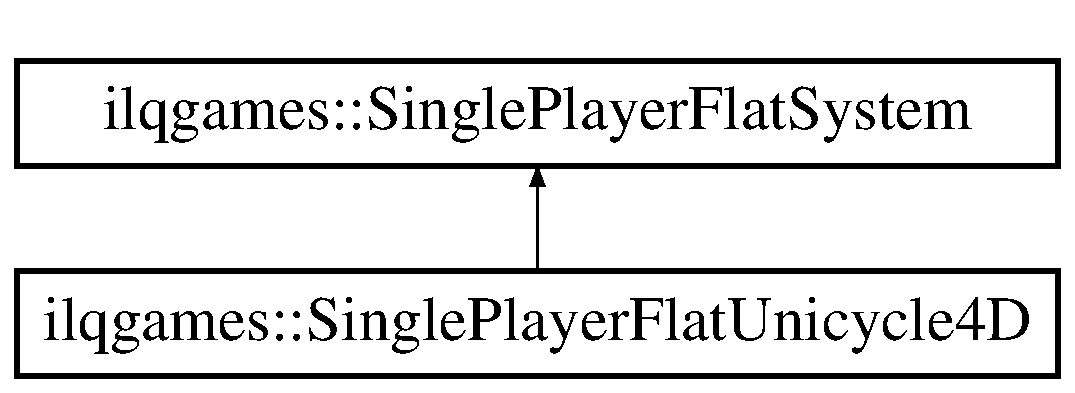
\includegraphics[height=2.000000cm]{classilqgames_1_1_single_player_flat_unicycle4_d}
\end{center}
\end{figure}
\subsection*{Public Member Functions}
\begin{DoxyCompactItemize}
\item 
Vector\+Xf {\bfseries Evaluate} (const Vector\+Xf \&x, const Vector\+Xf \&u) const \hypertarget{classilqgames_1_1_single_player_flat_unicycle4_d_a8cb7d02af4f2ca075a63c0277cbf1212}{}\label{classilqgames_1_1_single_player_flat_unicycle4_d_a8cb7d02af4f2ca075a63c0277cbf1212}

\item 
void {\bfseries Linearized\+System} (Eigen\+::\+Ref$<$ Matrix\+Xf $>$ A, Eigen\+::\+Ref$<$ Matrix\+Xf $>$ B) const \hypertarget{classilqgames_1_1_single_player_flat_unicycle4_d_a5c6ce1a0c4ed45269091a12d52bbbeab}{}\label{classilqgames_1_1_single_player_flat_unicycle4_d_a5c6ce1a0c4ed45269091a12d52bbbeab}

\item 
Matrix\+Xf {\bfseries Inverse\+Decoupling\+Matrix} (const Vector\+Xf \&x) const \hypertarget{classilqgames_1_1_single_player_flat_unicycle4_d_af5755f84b20abfed167035aa5380b19b}{}\label{classilqgames_1_1_single_player_flat_unicycle4_d_af5755f84b20abfed167035aa5380b19b}

\item 
Vector\+Xf {\bfseries Affine\+Term} (const Vector\+Xf \&x) const \hypertarget{classilqgames_1_1_single_player_flat_unicycle4_d_af7b121d4b464c453c125023f705557cf}{}\label{classilqgames_1_1_single_player_flat_unicycle4_d_af7b121d4b464c453c125023f705557cf}

\item 
Vector\+Xf {\bfseries To\+Linear\+System\+State} (const Vector\+Xf \&x) const \hypertarget{classilqgames_1_1_single_player_flat_unicycle4_d_abde027a03cb3886b23b89afd8dc789ed}{}\label{classilqgames_1_1_single_player_flat_unicycle4_d_abde027a03cb3886b23b89afd8dc789ed}

\item 
Vector\+Xf {\bfseries From\+Linear\+System\+State} (const Vector\+Xf \&xi) const \hypertarget{classilqgames_1_1_single_player_flat_unicycle4_d_ac0e69071e7afb0cbad008e032445abf7}{}\label{classilqgames_1_1_single_player_flat_unicycle4_d_ac0e69071e7afb0cbad008e032445abf7}

\item 
void {\bfseries Partial} (const Vector\+Xf \&xi, std\+::vector$<$ Vector\+Xf $>$ $\ast$grads, std\+::vector$<$ Matrix\+Xf $>$ $\ast$hesses) const \hypertarget{classilqgames_1_1_single_player_flat_unicycle4_d_a78781989d6608ca5004d67bfa14e643c}{}\label{classilqgames_1_1_single_player_flat_unicycle4_d_a78781989d6608ca5004d67bfa14e643c}

\item 
bool {\bfseries Is\+Linear\+System\+State\+Singular} (const Vector\+Xf \&xi) const \hypertarget{classilqgames_1_1_single_player_flat_unicycle4_d_aed29c096ed0b7d5a90bdda3663d27f48}{}\label{classilqgames_1_1_single_player_flat_unicycle4_d_aed29c096ed0b7d5a90bdda3663d27f48}

\item 
float {\bfseries Distance\+Between} (const Vector\+Xf \&x0, const Vector\+Xf \&x1) const \hypertarget{classilqgames_1_1_single_player_flat_unicycle4_d_a1ee1aefcf9dac3271e19759da30efada}{}\label{classilqgames_1_1_single_player_flat_unicycle4_d_a1ee1aefcf9dac3271e19759da30efada}

\item 
std\+::vector$<$ Dimension $>$ {\bfseries Position\+Dimensions} () const \hypertarget{classilqgames_1_1_single_player_flat_unicycle4_d_a949baca03af5ac51b8929f004b9fa60e}{}\label{classilqgames_1_1_single_player_flat_unicycle4_d_a949baca03af5ac51b8929f004b9fa60e}

\end{DoxyCompactItemize}
\subsection*{Static Public Attributes}
\begin{DoxyCompactItemize}
\item 
static const Dimension {\bfseries k\+Num\+X\+Dims} = 4\hypertarget{classilqgames_1_1_single_player_flat_unicycle4_d_a041e0a16201ec6acf1a5fdb864dd337f}{}\label{classilqgames_1_1_single_player_flat_unicycle4_d_a041e0a16201ec6acf1a5fdb864dd337f}

\item 
static const Dimension {\bfseries k\+Px\+Idx} = 0\hypertarget{classilqgames_1_1_single_player_flat_unicycle4_d_a811a52c424ad4ac644f515afddcf8a44}{}\label{classilqgames_1_1_single_player_flat_unicycle4_d_a811a52c424ad4ac644f515afddcf8a44}

\item 
static const Dimension {\bfseries k\+Py\+Idx} = 1\hypertarget{classilqgames_1_1_single_player_flat_unicycle4_d_abf9a17bc148226848151e65312ddc06c}{}\label{classilqgames_1_1_single_player_flat_unicycle4_d_abf9a17bc148226848151e65312ddc06c}

\item 
static const Dimension {\bfseries k\+Theta\+Idx} = 2\hypertarget{classilqgames_1_1_single_player_flat_unicycle4_d_a8574888ffd9f38ff34be962c44943c0f}{}\label{classilqgames_1_1_single_player_flat_unicycle4_d_a8574888ffd9f38ff34be962c44943c0f}

\item 
static const Dimension {\bfseries k\+V\+Idx} = 3\hypertarget{classilqgames_1_1_single_player_flat_unicycle4_d_acd6bca017ce205bce9aeb5665ed1aae0}{}\label{classilqgames_1_1_single_player_flat_unicycle4_d_acd6bca017ce205bce9aeb5665ed1aae0}

\item 
static const Dimension {\bfseries k\+Vx\+Idx} = 2\hypertarget{classilqgames_1_1_single_player_flat_unicycle4_d_a375c36dbc8e52637437fe99b5a9b2466}{}\label{classilqgames_1_1_single_player_flat_unicycle4_d_a375c36dbc8e52637437fe99b5a9b2466}

\item 
static const Dimension {\bfseries k\+Vy\+Idx} = 3\hypertarget{classilqgames_1_1_single_player_flat_unicycle4_d_a68b5611a53dd719e5eb978bee530ede6}{}\label{classilqgames_1_1_single_player_flat_unicycle4_d_a68b5611a53dd719e5eb978bee530ede6}

\item 
static const Dimension {\bfseries k\+Num\+U\+Dims} = 2\hypertarget{classilqgames_1_1_single_player_flat_unicycle4_d_a78e81e4a6c7dcd325b1e10f16408927e}{}\label{classilqgames_1_1_single_player_flat_unicycle4_d_a78e81e4a6c7dcd325b1e10f16408927e}

\item 
static const Dimension {\bfseries k\+Omega\+Idx} = 0\hypertarget{classilqgames_1_1_single_player_flat_unicycle4_d_aeb2485251d0e23f2d09e34bc75bf19aa}{}\label{classilqgames_1_1_single_player_flat_unicycle4_d_aeb2485251d0e23f2d09e34bc75bf19aa}

\item 
static const Dimension {\bfseries k\+A\+Idx} = 1\hypertarget{classilqgames_1_1_single_player_flat_unicycle4_d_a23e2e7c24651bc528073b81d42ef6a6f}{}\label{classilqgames_1_1_single_player_flat_unicycle4_d_a23e2e7c24651bc528073b81d42ef6a6f}

\end{DoxyCompactItemize}
\subsection*{Additional Inherited Members}


\subsection{Detailed Description}


Definition at line 62 of file single\+\_\+player\+\_\+flat\+\_\+unicycle\+\_\+4d.\+h.



The documentation for this class was generated from the following files\+:\begin{DoxyCompactItemize}
\item 
/home/travis/build/\+H\+J\+Reachability/ilqgames/include/ilqgames/dynamics/single\+\_\+player\+\_\+flat\+\_\+unicycle\+\_\+4d.\+h\item 
/home/travis/build/\+H\+J\+Reachability/ilqgames/src/single\+\_\+player\+\_\+flat\+\_\+unicycle\+\_\+4d.\+cpp\end{DoxyCompactItemize}

\hypertarget{classilqgames_1_1_single_player_unicycle4_d}{}\section{ilqgames\+:\+:Single\+Player\+Unicycle4D Class Reference}
\label{classilqgames_1_1_single_player_unicycle4_d}\index{ilqgames\+::\+Single\+Player\+Unicycle4D@{ilqgames\+::\+Single\+Player\+Unicycle4D}}
Inheritance diagram for ilqgames\+:\+:Single\+Player\+Unicycle4D\+:\begin{figure}[H]
\begin{center}
\leavevmode
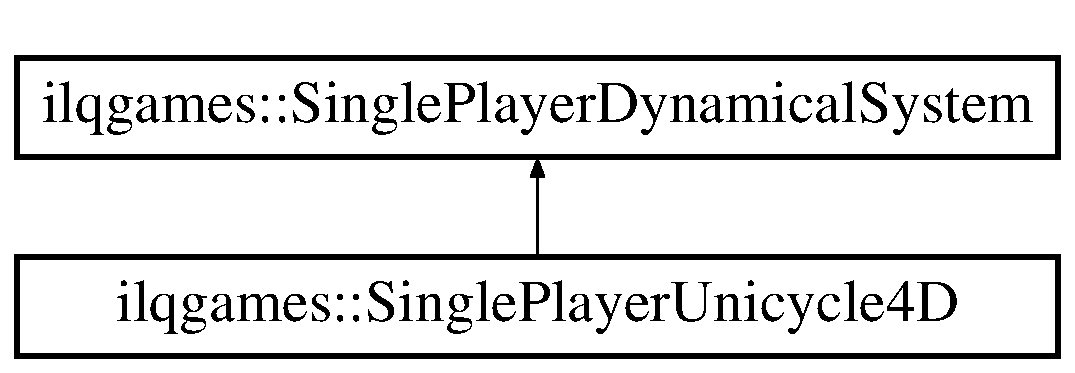
\includegraphics[height=2.000000cm]{classilqgames_1_1_single_player_unicycle4_d}
\end{center}
\end{figure}
\subsection*{Public Member Functions}
\begin{DoxyCompactItemize}
\item 
Vector\+Xf {\bfseries Evaluate} (Time t, const Vector\+Xf \&x, const Vector\+Xf \&u) const \hypertarget{classilqgames_1_1_single_player_unicycle4_d_a2d09bc46b962db25724fe381d44ecd5f}{}\label{classilqgames_1_1_single_player_unicycle4_d_a2d09bc46b962db25724fe381d44ecd5f}

\item 
void {\bfseries Linearize} (Time t, Time time\+\_\+step, const Vector\+Xf \&x, const Vector\+Xf \&u, Eigen\+::\+Ref$<$ Matrix\+Xf $>$ A, Eigen\+::\+Ref$<$ Matrix\+Xf $>$ B) const \hypertarget{classilqgames_1_1_single_player_unicycle4_d_a1b433ba55fba0620c251215e5927fe06}{}\label{classilqgames_1_1_single_player_unicycle4_d_a1b433ba55fba0620c251215e5927fe06}

\item 
float {\bfseries Distance\+Between} (const Vector\+Xf \&x0, const Vector\+Xf \&x1) const \hypertarget{classilqgames_1_1_single_player_unicycle4_d_a8e07e462f3b1efe63ae0f14ee286d657}{}\label{classilqgames_1_1_single_player_unicycle4_d_a8e07e462f3b1efe63ae0f14ee286d657}

\end{DoxyCompactItemize}
\subsection*{Static Public Attributes}
\begin{DoxyCompactItemize}
\item 
static const Dimension {\bfseries k\+Num\+X\+Dims} = 4\hypertarget{classilqgames_1_1_single_player_unicycle4_d_a5019976f8b6289615dfd81efdb61d015}{}\label{classilqgames_1_1_single_player_unicycle4_d_a5019976f8b6289615dfd81efdb61d015}

\item 
static const Dimension {\bfseries k\+Px\+Idx} = 0\hypertarget{classilqgames_1_1_single_player_unicycle4_d_a774ee86e4ac149f1f19f203189b88986}{}\label{classilqgames_1_1_single_player_unicycle4_d_a774ee86e4ac149f1f19f203189b88986}

\item 
static const Dimension {\bfseries k\+Py\+Idx} = 1\hypertarget{classilqgames_1_1_single_player_unicycle4_d_a2b5756708b8cd83784344c628418f08b}{}\label{classilqgames_1_1_single_player_unicycle4_d_a2b5756708b8cd83784344c628418f08b}

\item 
static const Dimension {\bfseries k\+Theta\+Idx} = 2\hypertarget{classilqgames_1_1_single_player_unicycle4_d_a9ef68c36855069eac6d1b70757b6e6ed}{}\label{classilqgames_1_1_single_player_unicycle4_d_a9ef68c36855069eac6d1b70757b6e6ed}

\item 
static const Dimension {\bfseries k\+V\+Idx} = 3\hypertarget{classilqgames_1_1_single_player_unicycle4_d_ab4ac2e584d119a1420fc9f7cb41242c6}{}\label{classilqgames_1_1_single_player_unicycle4_d_ab4ac2e584d119a1420fc9f7cb41242c6}

\item 
static const Dimension {\bfseries k\+Num\+U\+Dims} = 2\hypertarget{classilqgames_1_1_single_player_unicycle4_d_a8583fdc41b62a15f01f5b32b299f66fd}{}\label{classilqgames_1_1_single_player_unicycle4_d_a8583fdc41b62a15f01f5b32b299f66fd}

\item 
static const Dimension {\bfseries k\+Omega\+Idx} = 0\hypertarget{classilqgames_1_1_single_player_unicycle4_d_a6fa1e105146a0bc44eef48315cb2736c}{}\label{classilqgames_1_1_single_player_unicycle4_d_a6fa1e105146a0bc44eef48315cb2736c}

\item 
static const Dimension {\bfseries k\+A\+Idx} = 1\hypertarget{classilqgames_1_1_single_player_unicycle4_d_a0bdb794bca743c36ea5efb93778727b0}{}\label{classilqgames_1_1_single_player_unicycle4_d_a0bdb794bca743c36ea5efb93778727b0}

\end{DoxyCompactItemize}
\subsection*{Additional Inherited Members}


\subsection{Detailed Description}


Definition at line 56 of file single\+\_\+player\+\_\+unicycle\+\_\+4d.\+h.



The documentation for this class was generated from the following files\+:\begin{DoxyCompactItemize}
\item 
/home/travis/build/\+H\+J\+Reachability/ilqgames/include/ilqgames/dynamics/single\+\_\+player\+\_\+unicycle\+\_\+4d.\+h\item 
/home/travis/build/\+H\+J\+Reachability/ilqgames/src/single\+\_\+player\+\_\+unicycle\+\_\+4d.\+cpp\end{DoxyCompactItemize}

\hypertarget{classilqgames_1_1_single_player_unicycle5_d}{}\section{ilqgames\+:\+:Single\+Player\+Unicycle5D Class Reference}
\label{classilqgames_1_1_single_player_unicycle5_d}\index{ilqgames\+::\+Single\+Player\+Unicycle5D@{ilqgames\+::\+Single\+Player\+Unicycle5D}}
Inheritance diagram for ilqgames\+:\+:Single\+Player\+Unicycle5D\+:\begin{figure}[H]
\begin{center}
\leavevmode
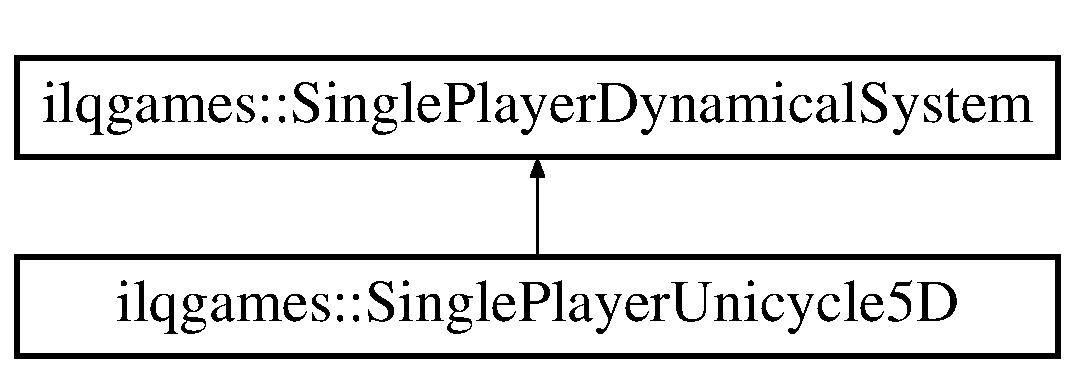
\includegraphics[height=2.000000cm]{classilqgames_1_1_single_player_unicycle5_d}
\end{center}
\end{figure}
\subsection*{Public Member Functions}
\begin{DoxyCompactItemize}
\item 
Vector\+Xf {\bfseries Evaluate} (Time t, const Vector\+Xf \&x, const Vector\+Xf \&u) const \hypertarget{classilqgames_1_1_single_player_unicycle5_d_a51f0dd94b0872632256ab0e31b760569}{}\label{classilqgames_1_1_single_player_unicycle5_d_a51f0dd94b0872632256ab0e31b760569}

\item 
void {\bfseries Linearize} (Time t, Time time\+\_\+step, const Vector\+Xf \&x, const Vector\+Xf \&u, Eigen\+::\+Ref$<$ Matrix\+Xf $>$ A, Eigen\+::\+Ref$<$ Matrix\+Xf $>$ B) const \hypertarget{classilqgames_1_1_single_player_unicycle5_d_abdfb1b8da8b6a60deacd6de1e2370264}{}\label{classilqgames_1_1_single_player_unicycle5_d_abdfb1b8da8b6a60deacd6de1e2370264}

\item 
float {\bfseries Distance\+Between} (const Vector\+Xf \&x0, const Vector\+Xf \&x1) const \hypertarget{classilqgames_1_1_single_player_unicycle5_d_ac20c427901e0e594d63155d0d7944b70}{}\label{classilqgames_1_1_single_player_unicycle5_d_ac20c427901e0e594d63155d0d7944b70}

\item 
std\+::vector$<$ Dimension $>$ {\bfseries Position\+Dimensions} () const \hypertarget{classilqgames_1_1_single_player_unicycle5_d_a0245cb33ac6ed95ce5331692c36e2a0d}{}\label{classilqgames_1_1_single_player_unicycle5_d_a0245cb33ac6ed95ce5331692c36e2a0d}

\end{DoxyCompactItemize}
\subsection*{Static Public Attributes}
\begin{DoxyCompactItemize}
\item 
static const Dimension {\bfseries k\+Num\+X\+Dims} = 5\hypertarget{classilqgames_1_1_single_player_unicycle5_d_a3de1934452ce10f5ff42ac82e754c911}{}\label{classilqgames_1_1_single_player_unicycle5_d_a3de1934452ce10f5ff42ac82e754c911}

\item 
static const Dimension {\bfseries k\+Px\+Idx} = 0\hypertarget{classilqgames_1_1_single_player_unicycle5_d_ad68ceaae295286eeb35f23f884b1cb4e}{}\label{classilqgames_1_1_single_player_unicycle5_d_ad68ceaae295286eeb35f23f884b1cb4e}

\item 
static const Dimension {\bfseries k\+Py\+Idx} = 1\hypertarget{classilqgames_1_1_single_player_unicycle5_d_aeb6d5a175a13af9b269bb429c2927c6b}{}\label{classilqgames_1_1_single_player_unicycle5_d_aeb6d5a175a13af9b269bb429c2927c6b}

\item 
static const Dimension {\bfseries k\+Theta\+Idx} = 2\hypertarget{classilqgames_1_1_single_player_unicycle5_d_a3420df6edf301a824f7eec4018d096a2}{}\label{classilqgames_1_1_single_player_unicycle5_d_a3420df6edf301a824f7eec4018d096a2}

\item 
static const Dimension {\bfseries k\+V\+Idx} = 3\hypertarget{classilqgames_1_1_single_player_unicycle5_d_a0a6cce244a9b0878bbf1cebdf93ae66a}{}\label{classilqgames_1_1_single_player_unicycle5_d_a0a6cce244a9b0878bbf1cebdf93ae66a}

\item 
static const Dimension {\bfseries k\+S\+Idx} = 4\hypertarget{classilqgames_1_1_single_player_unicycle5_d_ae695d4c4fdd88f13cd7aa7979b369f49}{}\label{classilqgames_1_1_single_player_unicycle5_d_ae695d4c4fdd88f13cd7aa7979b369f49}

\item 
static const Dimension {\bfseries k\+Num\+U\+Dims} = 2\hypertarget{classilqgames_1_1_single_player_unicycle5_d_a85a388fcb63f56b0bf28f715e93654cc}{}\label{classilqgames_1_1_single_player_unicycle5_d_a85a388fcb63f56b0bf28f715e93654cc}

\item 
static const Dimension {\bfseries k\+Omega\+Idx} = 0\hypertarget{classilqgames_1_1_single_player_unicycle5_d_accce3e20936b7b721735a917d20131a1}{}\label{classilqgames_1_1_single_player_unicycle5_d_accce3e20936b7b721735a917d20131a1}

\item 
static const Dimension {\bfseries k\+A\+Idx} = 1\hypertarget{classilqgames_1_1_single_player_unicycle5_d_a04d209e6ee6b880bcccc34c637df34cd}{}\label{classilqgames_1_1_single_player_unicycle5_d_a04d209e6ee6b880bcccc34c637df34cd}

\end{DoxyCompactItemize}
\subsection*{Additional Inherited Members}


\subsection{Detailed Description}


Definition at line 57 of file single\+\_\+player\+\_\+unicycle\+\_\+5d.\+h.



The documentation for this class was generated from the following files\+:\begin{DoxyCompactItemize}
\item 
/home/travis/build/\+H\+J\+Reachability/ilqgames/include/ilqgames/dynamics/single\+\_\+player\+\_\+unicycle\+\_\+5d.\+h\item 
/home/travis/build/\+H\+J\+Reachability/ilqgames/src/single\+\_\+player\+\_\+unicycle\+\_\+5d.\+cpp\end{DoxyCompactItemize}

\hypertarget{classilqgames_1_1_skeleton_example}{}\section{ilqgames\+:\+:Skeleton\+Example Class Reference}
\label{classilqgames_1_1_skeleton_example}\index{ilqgames\+::\+Skeleton\+Example@{ilqgames\+::\+Skeleton\+Example}}
Inheritance diagram for ilqgames\+:\+:Skeleton\+Example\+:\begin{figure}[H]
\begin{center}
\leavevmode
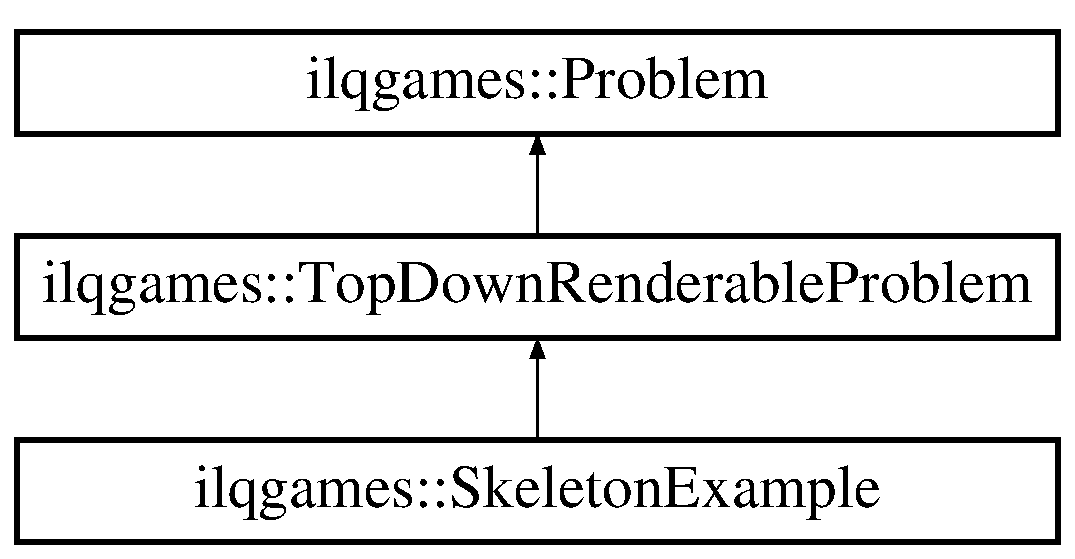
\includegraphics[height=3.000000cm]{classilqgames_1_1_skeleton_example}
\end{center}
\end{figure}
\subsection*{Public Member Functions}
\begin{DoxyCompactItemize}
\item 
{\bfseries Skeleton\+Example} (const \hyperlink{structilqgames_1_1_solver_params}{Solver\+Params} \&params)\hypertarget{classilqgames_1_1_skeleton_example_ad1700a16c9e56f80ca2e5ada926ccf72}{}\label{classilqgames_1_1_skeleton_example_ad1700a16c9e56f80ca2e5ada926ccf72}

\item 
std\+::vector$<$ float $>$ {\bfseries Xs} (const Vector\+Xf \&x) const \hypertarget{classilqgames_1_1_skeleton_example_ae0e9ad0a27e485e28e9ca3728df72470}{}\label{classilqgames_1_1_skeleton_example_ae0e9ad0a27e485e28e9ca3728df72470}

\item 
std\+::vector$<$ float $>$ {\bfseries Ys} (const Vector\+Xf \&x) const \hypertarget{classilqgames_1_1_skeleton_example_a09b34bb53952b9d151d61e94e8471fe4}{}\label{classilqgames_1_1_skeleton_example_a09b34bb53952b9d151d61e94e8471fe4}

\item 
std\+::vector$<$ float $>$ {\bfseries Thetas} (const Vector\+Xf \&x) const \hypertarget{classilqgames_1_1_skeleton_example_a3f62282748531798d1f821d8e937f2c6}{}\label{classilqgames_1_1_skeleton_example_a3f62282748531798d1f821d8e937f2c6}

\end{DoxyCompactItemize}
\subsection*{Additional Inherited Members}


\subsection{Detailed Description}


Definition at line 54 of file skeleton\+\_\+example.\+h.



The documentation for this class was generated from the following files\+:\begin{DoxyCompactItemize}
\item 
/home/travis/build/\+H\+J\+Reachability/ilqgames/include/ilqgames/examples/skeleton\+\_\+example.\+h\item 
/home/travis/build/\+H\+J\+Reachability/ilqgames/src/skeleton\+\_\+example.\+cpp\end{DoxyCompactItemize}

\hypertarget{classilqgames_1_1_solution_splicer}{}\section{ilqgames\+:\+:Solution\+Splicer Class Reference}
\label{classilqgames_1_1_solution_splicer}\index{ilqgames\+::\+Solution\+Splicer@{ilqgames\+::\+Solution\+Splicer}}
\subsection*{Public Member Functions}
\begin{DoxyCompactItemize}
\item 
{\bfseries Solution\+Splicer} (const \hyperlink{classilqgames_1_1_solver_log}{Solver\+Log} \&log)\hypertarget{classilqgames_1_1_solution_splicer_add264f103d0c16f989549ba4d030d13e}{}\label{classilqgames_1_1_solution_splicer_add264f103d0c16f989549ba4d030d13e}

\item 
void {\bfseries Splice} (const \hyperlink{classilqgames_1_1_solver_log}{Solver\+Log} \&log)\hypertarget{classilqgames_1_1_solution_splicer_aa6bd79330a78aa8627b08a0c855dc55b}{}\label{classilqgames_1_1_solution_splicer_aa6bd79330a78aa8627b08a0c855dc55b}

\item 
bool {\bfseries Contains\+Time} (Time t) const \hypertarget{classilqgames_1_1_solution_splicer_afdf52bb769bf720a8ee684013e89244f}{}\label{classilqgames_1_1_solution_splicer_afdf52bb769bf720a8ee684013e89244f}

\item 
const std\+::vector$<$ \hyperlink{structilqgames_1_1_strategy}{Strategy} $>$ \& {\bfseries Current\+Strategies} () const \hypertarget{classilqgames_1_1_solution_splicer_ab513525045570c0156ce8855fbe49871}{}\label{classilqgames_1_1_solution_splicer_ab513525045570c0156ce8855fbe49871}

\item 
const \hyperlink{structilqgames_1_1_operating_point}{Operating\+Point} \& {\bfseries Current\+Operating\+Point} () const \hypertarget{classilqgames_1_1_solution_splicer_aa9986a86a6dead3dbe781c6dfa5d6745}{}\label{classilqgames_1_1_solution_splicer_aa9986a86a6dead3dbe781c6dfa5d6745}

\end{DoxyCompactItemize}


\subsection{Detailed Description}


Definition at line 57 of file solution\+\_\+splicer.\+h.



The documentation for this class was generated from the following files\+:\begin{DoxyCompactItemize}
\item 
/home/travis/build/\+H\+J\+Reachability/ilqgames/include/ilqgames/solver/solution\+\_\+splicer.\+h\item 
/home/travis/build/\+H\+J\+Reachability/ilqgames/src/solution\+\_\+splicer.\+cpp\end{DoxyCompactItemize}

\hypertarget{classilqgames_1_1_solver_log}{}\section{ilqgames\+:\+:Solver\+Log Class Reference}
\label{classilqgames_1_1_solver_log}\index{ilqgames\+::\+Solver\+Log@{ilqgames\+::\+Solver\+Log}}
Inheritance diagram for ilqgames\+:\+:Solver\+Log\+:\begin{figure}[H]
\begin{center}
\leavevmode
\includegraphics[height=2.000000cm]{classilqgames_1_1_solver_log}
\end{center}
\end{figure}
\subsection*{Public Member Functions}
\begin{DoxyCompactItemize}
\item 
void {\bfseries Add\+Solver\+Iterate} (const \hyperlink{structilqgames_1_1_operating_point}{Operating\+Point} \&operating\+\_\+point, const std\+::vector$<$ \hyperlink{structilqgames_1_1_strategy}{Strategy} $>$ \&strategies, const std\+::vector$<$ float $>$ \&total\+\_\+costs, Time cumulative\+\_\+runtime, bool was\+\_\+converged)\hypertarget{classilqgames_1_1_solver_log_abbd4f1c7a064c3ae772633762d60a11e}{}\label{classilqgames_1_1_solver_log_abbd4f1c7a064c3ae772633762d60a11e}

\item 
void {\bfseries Add\+Log} (const \hyperlink{classilqgames_1_1_solver_log}{Solver\+Log} \&log)\hypertarget{classilqgames_1_1_solver_log_ae0b4da5de15e8a03a0c64e79db9fb60d}{}\label{classilqgames_1_1_solver_log_ae0b4da5de15e8a03a0c64e79db9fb60d}

\item 
void {\bfseries Clear\+All\+But\+First\+Iterate} ()\hypertarget{classilqgames_1_1_solver_log_aeb7c725598ed426c4428bd51ceaa0931}{}\label{classilqgames_1_1_solver_log_aeb7c725598ed426c4428bd51ceaa0931}

\item 
bool {\bfseries Was\+Converged} () const \hypertarget{classilqgames_1_1_solver_log_a1555d4b57427b3449c28e87a4b999905}{}\label{classilqgames_1_1_solver_log_a1555d4b57427b3449c28e87a4b999905}

\item 
bool {\bfseries Was\+Converged} (size\+\_\+t idx) const \hypertarget{classilqgames_1_1_solver_log_ace7a4654de1ca7e4250ebe3a93adad28}{}\label{classilqgames_1_1_solver_log_ace7a4654de1ca7e4250ebe3a93adad28}

\item 
Time {\bfseries Initial\+Time} () const \hypertarget{classilqgames_1_1_solver_log_aaaf83583b07bc9b9974ff0a21b11129b}{}\label{classilqgames_1_1_solver_log_aaaf83583b07bc9b9974ff0a21b11129b}

\item 
Time {\bfseries Final\+Time} () const \hypertarget{classilqgames_1_1_solver_log_a7d4f0d183aaa7f5a0a0818a301f4994f}{}\label{classilqgames_1_1_solver_log_a7d4f0d183aaa7f5a0a0818a301f4994f}

\item 
Player\+Index {\bfseries Num\+Players} () const \hypertarget{classilqgames_1_1_solver_log_af2b335909e75f63a910f4f734890d4d7}{}\label{classilqgames_1_1_solver_log_af2b335909e75f63a910f4f734890d4d7}

\item 
size\+\_\+t {\bfseries Num\+Iterates} () const \hypertarget{classilqgames_1_1_solver_log_a205590ee3aadd88aaf11ef6b5bb774dc}{}\label{classilqgames_1_1_solver_log_a205590ee3aadd88aaf11ef6b5bb774dc}

\item 
std\+::vector$<$ float $>$ {\bfseries Total\+Costs} () const \hypertarget{classilqgames_1_1_solver_log_a175236dc1d4d3028511b0c82500095c5}{}\label{classilqgames_1_1_solver_log_a175236dc1d4d3028511b0c82500095c5}

\item 
const std\+::vector$<$ \hyperlink{structilqgames_1_1_strategy}{Strategy} $>$ \& {\bfseries Initial\+Strategies} () const \hypertarget{classilqgames_1_1_solver_log_a2ac6ab2634e314d3eb7cc556850d7636}{}\label{classilqgames_1_1_solver_log_a2ac6ab2634e314d3eb7cc556850d7636}

\item 
const \hyperlink{structilqgames_1_1_operating_point}{Operating\+Point} \& {\bfseries Initial\+Operating\+Point} () const \hypertarget{classilqgames_1_1_solver_log_adf4581a26df80a6b69458f2d4f84deac}{}\label{classilqgames_1_1_solver_log_adf4581a26df80a6b69458f2d4f84deac}

\item 
const std\+::vector$<$ \hyperlink{structilqgames_1_1_strategy}{Strategy} $>$ \& {\bfseries Final\+Strategies} () const \hypertarget{classilqgames_1_1_solver_log_a3e998ebe01b5437dbea33c1e32739cbe}{}\label{classilqgames_1_1_solver_log_a3e998ebe01b5437dbea33c1e32739cbe}

\item 
const \hyperlink{structilqgames_1_1_operating_point}{Operating\+Point} \& {\bfseries Final\+Operating\+Point} () const \hypertarget{classilqgames_1_1_solver_log_ac02232ae7fa57715bc0b1795f4dd059f}{}\label{classilqgames_1_1_solver_log_ac02232ae7fa57715bc0b1795f4dd059f}

\item 
Vector\+Xf {\bfseries Interpolate\+State} (size\+\_\+t iterate, Time t) const \hypertarget{classilqgames_1_1_solver_log_a86b8dd605c03955a6fbafa2dc0b2a341}{}\label{classilqgames_1_1_solver_log_a86b8dd605c03955a6fbafa2dc0b2a341}

\item 
float {\bfseries Interpolate\+State} (size\+\_\+t iterate, Time t, Dimension dim) const \hypertarget{classilqgames_1_1_solver_log_ac81714a5caf9e2f497ed04b58e333757}{}\label{classilqgames_1_1_solver_log_ac81714a5caf9e2f497ed04b58e333757}

\item 
Vector\+Xf {\bfseries Interpolate\+Control} (size\+\_\+t iterate, Time t, Player\+Index player) const \hypertarget{classilqgames_1_1_solver_log_ac7d6053a5764889fca2ec5cf5a462988}{}\label{classilqgames_1_1_solver_log_ac7d6053a5764889fca2ec5cf5a462988}

\item 
float {\bfseries Interpolate\+Control} (size\+\_\+t iterate, Time t, Player\+Index player, Dimension dim) const \hypertarget{classilqgames_1_1_solver_log_af8fd1063450f96fa3e5029bc07b5b39b}{}\label{classilqgames_1_1_solver_log_af8fd1063450f96fa3e5029bc07b5b39b}

\item 
std\+::vector$<$ Matrix\+Xf $>$ {\bfseries Ps} (size\+\_\+t iterate, size\+\_\+t time\+\_\+index) const \hypertarget{classilqgames_1_1_solver_log_a5429c067fefb9d902be11cb881247a81}{}\label{classilqgames_1_1_solver_log_a5429c067fefb9d902be11cb881247a81}

\item 
std\+::vector$<$ Vector\+Xf $>$ {\bfseries alphas} (size\+\_\+t iterate, size\+\_\+t time\+\_\+index) const \hypertarget{classilqgames_1_1_solver_log_ae4725b1be8df5cb17312e8bb27bf1954}{}\label{classilqgames_1_1_solver_log_ae4725b1be8df5cb17312e8bb27bf1954}

\item 
Matrix\+Xf {\bfseries P} (size\+\_\+t iterate, size\+\_\+t time\+\_\+index, Player\+Index player) const \hypertarget{classilqgames_1_1_solver_log_a0bf49939b8e4b940067bf2157c621c93}{}\label{classilqgames_1_1_solver_log_a0bf49939b8e4b940067bf2157c621c93}

\item 
Vector\+Xf {\bfseries alpha} (size\+\_\+t iterate, size\+\_\+t time\+\_\+index, Player\+Index player) const \hypertarget{classilqgames_1_1_solver_log_a0234745c13f7426545dcf37ef759f7e3}{}\label{classilqgames_1_1_solver_log_a0234745c13f7426545dcf37ef759f7e3}

\item 
Vector\+Xf {\bfseries State} (size\+\_\+t iterate, size\+\_\+t time\+\_\+index) const \hypertarget{classilqgames_1_1_solver_log_a54b12edccfcfca015670cd6405b1b527}{}\label{classilqgames_1_1_solver_log_a54b12edccfcfca015670cd6405b1b527}

\item 
float {\bfseries State} (size\+\_\+t iterate, size\+\_\+t time\+\_\+index, Dimension dim) const \hypertarget{classilqgames_1_1_solver_log_a448f9cd63c6b6e889cb8791bc1902305}{}\label{classilqgames_1_1_solver_log_a448f9cd63c6b6e889cb8791bc1902305}

\item 
Vector\+Xf {\bfseries Control} (size\+\_\+t iterate, size\+\_\+t time\+\_\+index, Player\+Index player) const \hypertarget{classilqgames_1_1_solver_log_a7bfdf2a7a7ced357eafcd36e009425d3}{}\label{classilqgames_1_1_solver_log_a7bfdf2a7a7ced357eafcd36e009425d3}

\item 
float {\bfseries Control} (size\+\_\+t iterate, size\+\_\+t time\+\_\+index, Player\+Index player, Dimension dim) const \hypertarget{classilqgames_1_1_solver_log_a73a740dd13e6f8c3c8359294e7662687}{}\label{classilqgames_1_1_solver_log_a73a740dd13e6f8c3c8359294e7662687}

\item 
std\+::vector$<$ Matrix\+Xf $>$ {\bfseries Ps} (size\+\_\+t iterate, Time t) const \hypertarget{classilqgames_1_1_solver_log_ae958cea078e821259eed40c26904bfbf}{}\label{classilqgames_1_1_solver_log_ae958cea078e821259eed40c26904bfbf}

\item 
std\+::vector$<$ Vector\+Xf $>$ {\bfseries alphas} (size\+\_\+t iterate, Time t) const \hypertarget{classilqgames_1_1_solver_log_a995476b2148f34878345d42ab9fbbc53}{}\label{classilqgames_1_1_solver_log_a995476b2148f34878345d42ab9fbbc53}

\item 
Matrix\+Xf {\bfseries P} (size\+\_\+t iterate, Time t, Player\+Index player) const \hypertarget{classilqgames_1_1_solver_log_a9074054ada0fbcc9b59b073d65252dd7}{}\label{classilqgames_1_1_solver_log_a9074054ada0fbcc9b59b073d65252dd7}

\item 
Vector\+Xf {\bfseries alpha} (size\+\_\+t iterate, Time t, Player\+Index player) const \hypertarget{classilqgames_1_1_solver_log_ac621cbe5639cf7ed168677404311efed}{}\label{classilqgames_1_1_solver_log_ac621cbe5639cf7ed168677404311efed}

\item 
size\+\_\+t {\bfseries Time\+To\+Index} (Time t) const \hypertarget{classilqgames_1_1_solver_log_ac4e09ac795276835d047795ff4ebffc7}{}\label{classilqgames_1_1_solver_log_ac4e09ac795276835d047795ff4ebffc7}

\item 
Time {\bfseries Index\+To\+Time} (size\+\_\+t idx) const \hypertarget{classilqgames_1_1_solver_log_a5ab947d807b26ae2f10663e34af24f23}{}\label{classilqgames_1_1_solver_log_a5ab947d807b26ae2f10663e34af24f23}

\item 
bool {\bfseries Save} (bool only\+\_\+last\+\_\+trajectory=false, const std\+::string \&experiment\+\_\+name=Default\+Experiment\+Name()) const \hypertarget{classilqgames_1_1_solver_log_a28367e891af240b563417a8bd6c8127e}{}\label{classilqgames_1_1_solver_log_a28367e891af240b563417a8bd6c8127e}

\end{DoxyCompactItemize}


\subsection{Detailed Description}


Definition at line 59 of file solver\+\_\+log.\+h.



The documentation for this class was generated from the following files\+:\begin{DoxyCompactItemize}
\item 
/home/travis/build/\+H\+J\+Reachability/ilqgames/include/ilqgames/utils/solver\+\_\+log.\+h\item 
/home/travis/build/\+H\+J\+Reachability/ilqgames/src/solver\+\_\+log.\+cpp\end{DoxyCompactItemize}

\hypertarget{structilqgames_1_1_solver_params}{}\section{ilqgames\+:\+:Solver\+Params Struct Reference}
\label{structilqgames_1_1_solver_params}\index{ilqgames\+::\+Solver\+Params@{ilqgames\+::\+Solver\+Params}}
\subsection*{Public Attributes}
\begin{DoxyCompactItemize}
\item 
float {\bfseries convergence\+\_\+tolerance} = 1e-\/1\hypertarget{structilqgames_1_1_solver_params_afe3985198f617a446e43e3d3a3c6ed2e}{}\label{structilqgames_1_1_solver_params_afe3985198f617a446e43e3d3a3c6ed2e}

\item 
size\+\_\+t {\bfseries max\+\_\+solver\+\_\+iters} = 1000\hypertarget{structilqgames_1_1_solver_params_a525076d6ad3f90a2fc5c410d88dc090f}{}\label{structilqgames_1_1_solver_params_a525076d6ad3f90a2fc5c410d88dc090f}

\item 
bool {\bfseries linesearch} = true\hypertarget{structilqgames_1_1_solver_params_af5c0bdc01591507e9a83f686a5be8e49}{}\label{structilqgames_1_1_solver_params_af5c0bdc01591507e9a83f686a5be8e49}

\item 
float {\bfseries initial\+\_\+alpha\+\_\+scaling} = 0.\+5\hypertarget{structilqgames_1_1_solver_params_ac4b00024e1a74f611a0aeacbcdf91719}{}\label{structilqgames_1_1_solver_params_ac4b00024e1a74f611a0aeacbcdf91719}

\item 
float {\bfseries geometric\+\_\+alpha\+\_\+scaling} = 0.\+5\hypertarget{structilqgames_1_1_solver_params_a36f6667fd24a5c763c6e03f67acbbcb8}{}\label{structilqgames_1_1_solver_params_a36f6667fd24a5c763c6e03f67acbbcb8}

\item 
size\+\_\+t {\bfseries max\+\_\+backtracking\+\_\+steps} = 10\hypertarget{structilqgames_1_1_solver_params_ad130123c76a7b90d41cf836e275dfef0}{}\label{structilqgames_1_1_solver_params_ad130123c76a7b90d41cf836e275dfef0}

\item 
float {\bfseries trust\+\_\+region\+\_\+size} = 10.\+0\hypertarget{structilqgames_1_1_solver_params_af6f8750a857ace4ecb52e85fb7d04021}{}\label{structilqgames_1_1_solver_params_af6f8750a857ace4ecb52e85fb7d04021}

\item 
std\+::vector$<$ Dimension $>$ {\bfseries trust\+\_\+region\+\_\+dimensions}\hypertarget{structilqgames_1_1_solver_params_a5d2025c32b094329c126777e53122a08}{}\label{structilqgames_1_1_solver_params_a5d2025c32b094329c126777e53122a08}

\end{DoxyCompactItemize}


\subsection{Detailed Description}


Definition at line 50 of file solver\+\_\+params.\+h.



The documentation for this struct was generated from the following file\+:\begin{DoxyCompactItemize}
\item 
/home/travis/build/\+H\+J\+Reachability/ilqgames/include/ilqgames/solver/solver\+\_\+params.\+h\end{DoxyCompactItemize}

\hypertarget{structilqgames_1_1_strategy}{}\section{ilqgames\+:\+:Strategy Struct Reference}
\label{structilqgames_1_1_strategy}\index{ilqgames\+::\+Strategy@{ilqgames\+::\+Strategy}}
\subsection*{Public Member Functions}
\begin{DoxyCompactItemize}
\item 
{\bfseries Strategy} (size\+\_\+t horizon, Dimension xdim, Dimension udim)\hypertarget{structilqgames_1_1_strategy_a60de8ff226997a36f83ffd157c868456}{}\label{structilqgames_1_1_strategy_a60de8ff226997a36f83ffd157c868456}

\item 
Vector\+Xf {\bfseries operator()} (size\+\_\+t time\+\_\+index, const Vector\+Xf \&delta\+\_\+x, const Vector\+Xf \&u\+\_\+ref) const \hypertarget{structilqgames_1_1_strategy_ab2c02755490cfb3d88a062d6b0412306}{}\label{structilqgames_1_1_strategy_ab2c02755490cfb3d88a062d6b0412306}

\end{DoxyCompactItemize}
\subsection*{Public Attributes}
\begin{DoxyCompactItemize}
\item 
std\+::vector$<$ Matrix\+Xf $>$ {\bfseries Ps}\hypertarget{structilqgames_1_1_strategy_a388b037f047ca7ae2070dec436100331}{}\label{structilqgames_1_1_strategy_a388b037f047ca7ae2070dec436100331}

\item 
std\+::vector$<$ Vector\+Xf $>$ {\bfseries alphas}\hypertarget{structilqgames_1_1_strategy_a23297cf741c8faf93010f24dca1ce582}{}\label{structilqgames_1_1_strategy_a23297cf741c8faf93010f24dca1ce582}

\end{DoxyCompactItemize}


\subsection{Detailed Description}


Definition at line 58 of file strategy.\+h.



The documentation for this struct was generated from the following file\+:\begin{DoxyCompactItemize}
\item 
/home/travis/build/\+H\+J\+Reachability/ilqgames/include/ilqgames/utils/strategy.\+h\end{DoxyCompactItemize}

\hypertarget{classilqgames_1_1_three_player_collision_avoidance_reachability_example}{}\section{ilqgames\+:\+:Three\+Player\+Collision\+Avoidance\+Reachability\+Example Class Reference}
\label{classilqgames_1_1_three_player_collision_avoidance_reachability_example}\index{ilqgames\+::\+Three\+Player\+Collision\+Avoidance\+Reachability\+Example@{ilqgames\+::\+Three\+Player\+Collision\+Avoidance\+Reachability\+Example}}
Inheritance diagram for ilqgames\+:\+:Three\+Player\+Collision\+Avoidance\+Reachability\+Example\+:\begin{figure}[H]
\begin{center}
\leavevmode
\includegraphics[height=3.000000cm]{classilqgames_1_1_three_player_collision_avoidance_reachability_example}
\end{center}
\end{figure}
\subsection*{Public Member Functions}
\begin{DoxyCompactItemize}
\item 
{\bfseries Three\+Player\+Collision\+Avoidance\+Reachability\+Example} (const \hyperlink{structilqgames_1_1_solver_params}{Solver\+Params} \&params)\hypertarget{classilqgames_1_1_three_player_collision_avoidance_reachability_example_a02ba0e88f32c81504311c8ef887b6d6b}{}\label{classilqgames_1_1_three_player_collision_avoidance_reachability_example_a02ba0e88f32c81504311c8ef887b6d6b}

\item 
std\+::vector$<$ float $>$ {\bfseries Xs} (const Vector\+Xf \&x) const \hypertarget{classilqgames_1_1_three_player_collision_avoidance_reachability_example_a2a84d8d679c389a2518e8a5831c77efe}{}\label{classilqgames_1_1_three_player_collision_avoidance_reachability_example_a2a84d8d679c389a2518e8a5831c77efe}

\item 
std\+::vector$<$ float $>$ {\bfseries Ys} (const Vector\+Xf \&x) const \hypertarget{classilqgames_1_1_three_player_collision_avoidance_reachability_example_af7e78eadcbfd56ae24a9ee7e89081f8c}{}\label{classilqgames_1_1_three_player_collision_avoidance_reachability_example_af7e78eadcbfd56ae24a9ee7e89081f8c}

\item 
std\+::vector$<$ float $>$ {\bfseries Thetas} (const Vector\+Xf \&x) const \hypertarget{classilqgames_1_1_three_player_collision_avoidance_reachability_example_a1563fa42643df8d229827c2055255070}{}\label{classilqgames_1_1_three_player_collision_avoidance_reachability_example_a1563fa42643df8d229827c2055255070}

\end{DoxyCompactItemize}
\subsection*{Additional Inherited Members}


\subsection{Detailed Description}


Definition at line 51 of file three\+\_\+player\+\_\+collision\+\_\+avoidance\+\_\+reachability\+\_\+example.\+h.



The documentation for this class was generated from the following files\+:\begin{DoxyCompactItemize}
\item 
/home/travis/build/\+H\+J\+Reachability/ilqgames/include/ilqgames/examples/three\+\_\+player\+\_\+collision\+\_\+avoidance\+\_\+reachability\+\_\+example.\+h\item 
/home/travis/build/\+H\+J\+Reachability/ilqgames/src/three\+\_\+player\+\_\+collision\+\_\+avoidance\+\_\+reachability\+\_\+example.\+cpp\end{DoxyCompactItemize}

\hypertarget{classilqgames_1_1_three_player_flat_intersection_example}{}\section{ilqgames\+:\+:Three\+Player\+Flat\+Intersection\+Example Class Reference}
\label{classilqgames_1_1_three_player_flat_intersection_example}\index{ilqgames\+::\+Three\+Player\+Flat\+Intersection\+Example@{ilqgames\+::\+Three\+Player\+Flat\+Intersection\+Example}}
Inheritance diagram for ilqgames\+:\+:Three\+Player\+Flat\+Intersection\+Example\+:\begin{figure}[H]
\begin{center}
\leavevmode
\includegraphics[height=3.000000cm]{classilqgames_1_1_three_player_flat_intersection_example}
\end{center}
\end{figure}
\subsection*{Public Member Functions}
\begin{DoxyCompactItemize}
\item 
{\bfseries Three\+Player\+Flat\+Intersection\+Example} (const \hyperlink{structilqgames_1_1_solver_params}{Solver\+Params} \&params)\hypertarget{classilqgames_1_1_three_player_flat_intersection_example_aa6a3e8264c12f5c0e424a2a801371a4e}{}\label{classilqgames_1_1_three_player_flat_intersection_example_aa6a3e8264c12f5c0e424a2a801371a4e}

\item 
std\+::vector$<$ float $>$ {\bfseries Xs} (const Vector\+Xf \&xi) const \hypertarget{classilqgames_1_1_three_player_flat_intersection_example_ad4c92ff703b198cf937df281f09d176a}{}\label{classilqgames_1_1_three_player_flat_intersection_example_ad4c92ff703b198cf937df281f09d176a}

\item 
std\+::vector$<$ float $>$ {\bfseries Ys} (const Vector\+Xf \&xi) const \hypertarget{classilqgames_1_1_three_player_flat_intersection_example_a5f60f5d993fec248893fcbda45aad15a}{}\label{classilqgames_1_1_three_player_flat_intersection_example_a5f60f5d993fec248893fcbda45aad15a}

\item 
std\+::vector$<$ float $>$ {\bfseries Thetas} (const Vector\+Xf \&xi) const \hypertarget{classilqgames_1_1_three_player_flat_intersection_example_aaffec79328bcd92dc2d5c8bd0aada196}{}\label{classilqgames_1_1_three_player_flat_intersection_example_aaffec79328bcd92dc2d5c8bd0aada196}

\item 
std\+::shared\+\_\+ptr$<$ const \hyperlink{classilqgames_1_1_multi_player_flat_system}{Multi\+Player\+Flat\+System} $>$ {\bfseries Dynamics} () const \hypertarget{classilqgames_1_1_three_player_flat_intersection_example_a2a4043278484419adf07ed5268453df3}{}\label{classilqgames_1_1_three_player_flat_intersection_example_a2a4043278484419adf07ed5268453df3}

\end{DoxyCompactItemize}
\subsection*{Additional Inherited Members}


\subsection{Detailed Description}


Definition at line 53 of file three\+\_\+player\+\_\+flat\+\_\+intersection\+\_\+example.\+h.



The documentation for this class was generated from the following files\+:\begin{DoxyCompactItemize}
\item 
/home/travis/build/\+H\+J\+Reachability/ilqgames/include/ilqgames/examples/three\+\_\+player\+\_\+flat\+\_\+intersection\+\_\+example.\+h\item 
/home/travis/build/\+H\+J\+Reachability/ilqgames/src/three\+\_\+player\+\_\+flat\+\_\+intersection\+\_\+example.\+cpp\end{DoxyCompactItemize}

\hypertarget{classilqgames_1_1_three_player_flat_overtaking_example}{}\section{ilqgames\+:\+:Three\+Player\+Flat\+Overtaking\+Example Class Reference}
\label{classilqgames_1_1_three_player_flat_overtaking_example}\index{ilqgames\+::\+Three\+Player\+Flat\+Overtaking\+Example@{ilqgames\+::\+Three\+Player\+Flat\+Overtaking\+Example}}
Inheritance diagram for ilqgames\+:\+:Three\+Player\+Flat\+Overtaking\+Example\+:\begin{figure}[H]
\begin{center}
\leavevmode
\includegraphics[height=3.000000cm]{classilqgames_1_1_three_player_flat_overtaking_example}
\end{center}
\end{figure}
\subsection*{Public Member Functions}
\begin{DoxyCompactItemize}
\item 
{\bfseries Three\+Player\+Flat\+Overtaking\+Example} (const \hyperlink{structilqgames_1_1_solver_params}{Solver\+Params} \&params)\hypertarget{classilqgames_1_1_three_player_flat_overtaking_example_a00b990b6c29657cb1516fd8132884036}{}\label{classilqgames_1_1_three_player_flat_overtaking_example_a00b990b6c29657cb1516fd8132884036}

\item 
std\+::vector$<$ float $>$ {\bfseries Xs} (const Vector\+Xf \&xi) const \hypertarget{classilqgames_1_1_three_player_flat_overtaking_example_a47a85425d31dd4a5e4d4534b9ff50c83}{}\label{classilqgames_1_1_three_player_flat_overtaking_example_a47a85425d31dd4a5e4d4534b9ff50c83}

\item 
std\+::vector$<$ float $>$ {\bfseries Ys} (const Vector\+Xf \&xi) const \hypertarget{classilqgames_1_1_three_player_flat_overtaking_example_ad4c1ae9db31f1f25c71187692d94b05d}{}\label{classilqgames_1_1_three_player_flat_overtaking_example_ad4c1ae9db31f1f25c71187692d94b05d}

\item 
std\+::vector$<$ float $>$ {\bfseries Thetas} (const Vector\+Xf \&xi) const \hypertarget{classilqgames_1_1_three_player_flat_overtaking_example_a92be7f8ef2b6ee6e6ac4339a32a30991}{}\label{classilqgames_1_1_three_player_flat_overtaking_example_a92be7f8ef2b6ee6e6ac4339a32a30991}

\item 
std\+::shared\+\_\+ptr$<$ const \hyperlink{classilqgames_1_1_multi_player_flat_system}{Multi\+Player\+Flat\+System} $>$ {\bfseries Dynamics} () const \hypertarget{classilqgames_1_1_three_player_flat_overtaking_example_a33fb0ea831db32f859718c7a54d80c6f}{}\label{classilqgames_1_1_three_player_flat_overtaking_example_a33fb0ea831db32f859718c7a54d80c6f}

\end{DoxyCompactItemize}
\subsection*{Additional Inherited Members}


\subsection{Detailed Description}


Definition at line 53 of file three\+\_\+player\+\_\+flat\+\_\+overtaking\+\_\+example.\+h.



The documentation for this class was generated from the following files\+:\begin{DoxyCompactItemize}
\item 
/home/travis/build/\+H\+J\+Reachability/ilqgames/include/ilqgames/examples/three\+\_\+player\+\_\+flat\+\_\+overtaking\+\_\+example.\+h\item 
/home/travis/build/\+H\+J\+Reachability/ilqgames/src/three\+\_\+player\+\_\+flat\+\_\+overtaking\+\_\+example.\+cpp\end{DoxyCompactItemize}

\hypertarget{classilqgames_1_1_three_player_intersection_example}{}\section{ilqgames\+:\+:Three\+Player\+Intersection\+Example Class Reference}
\label{classilqgames_1_1_three_player_intersection_example}\index{ilqgames\+::\+Three\+Player\+Intersection\+Example@{ilqgames\+::\+Three\+Player\+Intersection\+Example}}
Inheritance diagram for ilqgames\+:\+:Three\+Player\+Intersection\+Example\+:\begin{figure}[H]
\begin{center}
\leavevmode
\includegraphics[height=3.000000cm]{classilqgames_1_1_three_player_intersection_example}
\end{center}
\end{figure}
\subsection*{Public Member Functions}
\begin{DoxyCompactItemize}
\item 
{\bfseries Three\+Player\+Intersection\+Example} (const \hyperlink{structilqgames_1_1_solver_params}{Solver\+Params} \&params)\hypertarget{classilqgames_1_1_three_player_intersection_example_af9f970a8a99ed255a81a12fbcb4328af}{}\label{classilqgames_1_1_three_player_intersection_example_af9f970a8a99ed255a81a12fbcb4328af}

\item 
std\+::vector$<$ float $>$ {\bfseries Xs} (const Vector\+Xf \&x) const \hypertarget{classilqgames_1_1_three_player_intersection_example_ae81326cb33320fb55eac09dc009cdc26}{}\label{classilqgames_1_1_three_player_intersection_example_ae81326cb33320fb55eac09dc009cdc26}

\item 
std\+::vector$<$ float $>$ {\bfseries Ys} (const Vector\+Xf \&x) const \hypertarget{classilqgames_1_1_three_player_intersection_example_aeb38711ec9f6dd776ba359485f7e981a}{}\label{classilqgames_1_1_three_player_intersection_example_aeb38711ec9f6dd776ba359485f7e981a}

\item 
std\+::vector$<$ float $>$ {\bfseries Thetas} (const Vector\+Xf \&x) const \hypertarget{classilqgames_1_1_three_player_intersection_example_a74b3ff1cc6bbb27ea3e673792f623a61}{}\label{classilqgames_1_1_three_player_intersection_example_a74b3ff1cc6bbb27ea3e673792f623a61}

\end{DoxyCompactItemize}
\subsection*{Additional Inherited Members}


\subsection{Detailed Description}


Definition at line 52 of file three\+\_\+player\+\_\+intersection\+\_\+example.\+h.



The documentation for this class was generated from the following files\+:\begin{DoxyCompactItemize}
\item 
/home/travis/build/\+H\+J\+Reachability/ilqgames/include/ilqgames/examples/three\+\_\+player\+\_\+intersection\+\_\+example.\+h\item 
/home/travis/build/\+H\+J\+Reachability/ilqgames/src/three\+\_\+player\+\_\+intersection\+\_\+example.\+cpp\end{DoxyCompactItemize}

\hypertarget{classilqgames_1_1_three_player_overtaking_example}{}\section{ilqgames\+:\+:Three\+Player\+Overtaking\+Example Class Reference}
\label{classilqgames_1_1_three_player_overtaking_example}\index{ilqgames\+::\+Three\+Player\+Overtaking\+Example@{ilqgames\+::\+Three\+Player\+Overtaking\+Example}}
Inheritance diagram for ilqgames\+:\+:Three\+Player\+Overtaking\+Example\+:\begin{figure}[H]
\begin{center}
\leavevmode
\includegraphics[height=3.000000cm]{classilqgames_1_1_three_player_overtaking_example}
\end{center}
\end{figure}
\subsection*{Public Member Functions}
\begin{DoxyCompactItemize}
\item 
void {\bfseries Construct\+Dynamics} ()\hypertarget{classilqgames_1_1_three_player_overtaking_example_a0fa53d844b59aff3f1bf9f0091b97877}{}\label{classilqgames_1_1_three_player_overtaking_example_a0fa53d844b59aff3f1bf9f0091b97877}

\item 
void {\bfseries Construct\+Initial\+State} ()\hypertarget{classilqgames_1_1_three_player_overtaking_example_a63c729f7c8cd4e2818640c5e446927ef}{}\label{classilqgames_1_1_three_player_overtaking_example_a63c729f7c8cd4e2818640c5e446927ef}

\item 
void {\bfseries Construct\+Player\+Costs} ()\hypertarget{classilqgames_1_1_three_player_overtaking_example_a2799c3b06d3706a4ba9afcb7e67ff215}{}\label{classilqgames_1_1_three_player_overtaking_example_a2799c3b06d3706a4ba9afcb7e67ff215}

\item 
std\+::vector$<$ float $>$ {\bfseries Xs} (const Vector\+Xf \&x) const \hypertarget{classilqgames_1_1_three_player_overtaking_example_ae5d9261dd67bbb2091f767c0f733b52f}{}\label{classilqgames_1_1_three_player_overtaking_example_ae5d9261dd67bbb2091f767c0f733b52f}

\item 
std\+::vector$<$ float $>$ {\bfseries Ys} (const Vector\+Xf \&x) const \hypertarget{classilqgames_1_1_three_player_overtaking_example_a679b545d0d4ee9941fd1ed784702bbd2}{}\label{classilqgames_1_1_three_player_overtaking_example_a679b545d0d4ee9941fd1ed784702bbd2}

\item 
std\+::vector$<$ float $>$ {\bfseries Thetas} (const Vector\+Xf \&x) const \hypertarget{classilqgames_1_1_three_player_overtaking_example_ae93b1b20f879c3ee8c948baeacdca418}{}\label{classilqgames_1_1_three_player_overtaking_example_ae93b1b20f879c3ee8c948baeacdca418}

\end{DoxyCompactItemize}
\subsection*{Additional Inherited Members}


\subsection{Detailed Description}


Definition at line 52 of file three\+\_\+player\+\_\+overtaking\+\_\+example.\+h.



The documentation for this class was generated from the following files\+:\begin{DoxyCompactItemize}
\item 
/home/travis/build/\+H\+J\+Reachability/ilqgames/include/ilqgames/examples/three\+\_\+player\+\_\+overtaking\+\_\+example.\+h\item 
/home/travis/build/\+H\+J\+Reachability/ilqgames/src/three\+\_\+player\+\_\+overtaking\+\_\+example.\+cpp\end{DoxyCompactItemize}

\hypertarget{classilqgames_1_1_time_invariant_constraint}{}\section{ilqgames\+:\+:Time\+Invariant\+Constraint Class Reference}
\label{classilqgames_1_1_time_invariant_constraint}\index{ilqgames\+::\+Time\+Invariant\+Constraint@{ilqgames\+::\+Time\+Invariant\+Constraint}}
Inheritance diagram for ilqgames\+:\+:Time\+Invariant\+Constraint\+:\begin{figure}[H]
\begin{center}
\leavevmode
\includegraphics[height=2.755228cm]{classilqgames_1_1_time_invariant_constraint}
\end{center}
\end{figure}
\subsection*{Public Member Functions}
\begin{DoxyCompactItemize}
\item 
bool {\bfseries Is\+Satisfied\+Level} (Time t, const Vector\+Xf \&input, float $\ast$level) const \hypertarget{classilqgames_1_1_time_invariant_constraint_ab0efa7c3412a2340dcc277db4a869a35}{}\label{classilqgames_1_1_time_invariant_constraint_ab0efa7c3412a2340dcc277db4a869a35}

\item 
virtual bool {\bfseries Is\+Satisfied\+Level} (const Vector\+Xf \&input, float $\ast$level) const =0\hypertarget{classilqgames_1_1_time_invariant_constraint_a8e1a57ae94dc3a9f51c28f146e6c502d}{}\label{classilqgames_1_1_time_invariant_constraint_a8e1a57ae94dc3a9f51c28f146e6c502d}

\item 
float {\bfseries Evaluate} (const Vector\+Xf \&input) const \hypertarget{classilqgames_1_1_time_invariant_constraint_a2e1b3d7fbe55250677bfe61c394dd06f}{}\label{classilqgames_1_1_time_invariant_constraint_a2e1b3d7fbe55250677bfe61c394dd06f}

\item 
void {\bfseries Quadraticize} (Time t, const Vector\+Xf \&input, Matrix\+Xf $\ast$hess, Vector\+Xf $\ast$grad) const \hypertarget{classilqgames_1_1_time_invariant_constraint_ae8244c5a37225511e93a920126df8b7d}{}\label{classilqgames_1_1_time_invariant_constraint_ae8244c5a37225511e93a920126df8b7d}

\item 
virtual void {\bfseries Quadraticize} (const Vector\+Xf \&input, Matrix\+Xf $\ast$hess, Vector\+Xf $\ast$grad) const =0\hypertarget{classilqgames_1_1_time_invariant_constraint_a8ed31ed76064bf2a3a47e9f16be79d88}{}\label{classilqgames_1_1_time_invariant_constraint_a8ed31ed76064bf2a3a47e9f16be79d88}

\end{DoxyCompactItemize}
\subsection*{Protected Member Functions}
\begin{DoxyCompactItemize}
\item 
{\bfseries Time\+Invariant\+Constraint} (const std\+::string \&name=\char`\"{}\char`\"{})\hypertarget{classilqgames_1_1_time_invariant_constraint_a3e98eea0993ef95728ca804617b52d41}{}\label{classilqgames_1_1_time_invariant_constraint_a3e98eea0993ef95728ca804617b52d41}

\end{DoxyCompactItemize}
\subsection*{Additional Inherited Members}


\subsection{Detailed Description}


Definition at line 54 of file time\+\_\+invariant\+\_\+constraint.\+h.



The documentation for this class was generated from the following file\+:\begin{DoxyCompactItemize}
\item 
/home/travis/build/\+H\+J\+Reachability/ilqgames/include/ilqgames/constraint/time\+\_\+invariant\+\_\+constraint.\+h\end{DoxyCompactItemize}

\hypertarget{classilqgames_1_1_time_invariant_cost}{}\section{ilqgames\+:\+:Time\+Invariant\+Cost Class Reference}
\label{classilqgames_1_1_time_invariant_cost}\index{ilqgames\+::\+Time\+Invariant\+Cost@{ilqgames\+::\+Time\+Invariant\+Cost}}
Inheritance diagram for ilqgames\+:\+:Time\+Invariant\+Cost\+:\begin{figure}[H]
\begin{center}
\leavevmode
\includegraphics[height=12.000000cm]{classilqgames_1_1_time_invariant_cost}
\end{center}
\end{figure}
\subsection*{Public Member Functions}
\begin{DoxyCompactItemize}
\item 
virtual float {\bfseries Evaluate} (const Vector\+Xf \&input) const =0\hypertarget{classilqgames_1_1_time_invariant_cost_a61c214ac9833c3f42b51167bdec1cbc7}{}\label{classilqgames_1_1_time_invariant_cost_a61c214ac9833c3f42b51167bdec1cbc7}

\item 
float {\bfseries Evaluate} (Time t, const Vector\+Xf \&input) const \hypertarget{classilqgames_1_1_time_invariant_cost_a1e59c75a8765e4d89243c20838cc2bed}{}\label{classilqgames_1_1_time_invariant_cost_a1e59c75a8765e4d89243c20838cc2bed}

\item 
virtual void {\bfseries Quadraticize} (const Vector\+Xf \&input, Matrix\+Xf $\ast$hess, Vector\+Xf $\ast$grad) const =0\hypertarget{classilqgames_1_1_time_invariant_cost_abe3173385a2f31fa556c1553075eb18f}{}\label{classilqgames_1_1_time_invariant_cost_abe3173385a2f31fa556c1553075eb18f}

\item 
void {\bfseries Quadraticize} (Time t, const Vector\+Xf \&input, Matrix\+Xf $\ast$hess, Vector\+Xf $\ast$grad) const \hypertarget{classilqgames_1_1_time_invariant_cost_a185aa5080bcdaa68804810d1a046ebcd}{}\label{classilqgames_1_1_time_invariant_cost_a185aa5080bcdaa68804810d1a046ebcd}

\end{DoxyCompactItemize}
\subsection*{Protected Member Functions}
\begin{DoxyCompactItemize}
\item 
{\bfseries Time\+Invariant\+Cost} (float weight, const std\+::string \&name)\hypertarget{classilqgames_1_1_time_invariant_cost_a284519a634c47b5954f64349db1ede2e}{}\label{classilqgames_1_1_time_invariant_cost_a284519a634c47b5954f64349db1ede2e}

\end{DoxyCompactItemize}
\subsection*{Additional Inherited Members}


\subsection{Detailed Description}


Definition at line 53 of file time\+\_\+invariant\+\_\+cost.\+h.



The documentation for this class was generated from the following file\+:\begin{DoxyCompactItemize}
\item 
/home/travis/build/\+H\+J\+Reachability/ilqgames/include/ilqgames/cost/time\+\_\+invariant\+\_\+cost.\+h\end{DoxyCompactItemize}

\hypertarget{classilqgames_1_1_top_down_renderable_problem}{}\section{ilqgames\+:\+:Top\+Down\+Renderable\+Problem Class Reference}
\label{classilqgames_1_1_top_down_renderable_problem}\index{ilqgames\+::\+Top\+Down\+Renderable\+Problem@{ilqgames\+::\+Top\+Down\+Renderable\+Problem}}
Inheritance diagram for ilqgames\+:\+:Top\+Down\+Renderable\+Problem\+:\begin{figure}[H]
\begin{center}
\leavevmode
\includegraphics[height=12.000000cm]{classilqgames_1_1_top_down_renderable_problem}
\end{center}
\end{figure}
\subsection*{Public Member Functions}
\begin{DoxyCompactItemize}
\item 
virtual std\+::vector$<$ float $>$ {\bfseries Xs} (const Vector\+Xf \&x) const =0\hypertarget{classilqgames_1_1_top_down_renderable_problem_aecfc819c7a5f9f2a641fcfea8a96ce3b}{}\label{classilqgames_1_1_top_down_renderable_problem_aecfc819c7a5f9f2a641fcfea8a96ce3b}

\item 
virtual std\+::vector$<$ float $>$ {\bfseries Ys} (const Vector\+Xf \&x) const =0\hypertarget{classilqgames_1_1_top_down_renderable_problem_a702009371be24e0143afb1dbc80f46c4}{}\label{classilqgames_1_1_top_down_renderable_problem_a702009371be24e0143afb1dbc80f46c4}

\item 
virtual std\+::vector$<$ float $>$ {\bfseries Thetas} (const Vector\+Xf \&x) const =0\hypertarget{classilqgames_1_1_top_down_renderable_problem_a9f128739ad2503ae4e18b4ccfc0c8f33}{}\label{classilqgames_1_1_top_down_renderable_problem_a9f128739ad2503ae4e18b4ccfc0c8f33}

\end{DoxyCompactItemize}
\subsection*{Additional Inherited Members}


\subsection{Detailed Description}


Definition at line 51 of file top\+\_\+down\+\_\+renderable\+\_\+problem.\+h.



The documentation for this class was generated from the following file\+:\begin{DoxyCompactItemize}
\item 
/home/travis/build/\+H\+J\+Reachability/ilqgames/include/ilqgames/solver/top\+\_\+down\+\_\+renderable\+\_\+problem.\+h\end{DoxyCompactItemize}

\hypertarget{classilqgames_1_1_top_down_renderer}{}\section{ilqgames\+:\+:Top\+Down\+Renderer Class Reference}
\label{classilqgames_1_1_top_down_renderer}\index{ilqgames\+::\+Top\+Down\+Renderer@{ilqgames\+::\+Top\+Down\+Renderer}}
\subsection*{Public Member Functions}
\begin{DoxyCompactItemize}
\item 
{\bfseries Top\+Down\+Renderer} (const std\+::shared\+\_\+ptr$<$ const \hyperlink{classilqgames_1_1_control_sliders}{Control\+Sliders} $>$ \&sliders, const std\+::vector$<$ std\+::shared\+\_\+ptr$<$ const \hyperlink{classilqgames_1_1_solver_log}{Solver\+Log} $>$$>$ \&logs, const std\+::shared\+\_\+ptr$<$ const \hyperlink{classilqgames_1_1_top_down_renderable_problem}{Top\+Down\+Renderable\+Problem} $>$ \&problem)\hypertarget{classilqgames_1_1_top_down_renderer_a189aee6171b80a800f84b130e14e3f0c}{}\label{classilqgames_1_1_top_down_renderer_a189aee6171b80a800f84b130e14e3f0c}

\item 
void {\bfseries Render} ()\hypertarget{classilqgames_1_1_top_down_renderer_af50dc993130fbca96d4269e307bf2dae}{}\label{classilqgames_1_1_top_down_renderer_af50dc993130fbca96d4269e307bf2dae}

\end{DoxyCompactItemize}


\subsection{Detailed Description}


Definition at line 58 of file top\+\_\+down\+\_\+renderer.\+h.



The documentation for this class was generated from the following files\+:\begin{DoxyCompactItemize}
\item 
/home/travis/build/\+H\+J\+Reachability/ilqgames/include/ilqgames/gui/top\+\_\+down\+\_\+renderer.\+h\item 
/home/travis/build/\+H\+J\+Reachability/ilqgames/src/top\+\_\+down\+\_\+renderer.\+cpp\end{DoxyCompactItemize}

\hypertarget{classilqgames_1_1_two_player_collision_avoidance_reachability_example}{}\section{ilqgames\+:\+:Two\+Player\+Collision\+Avoidance\+Reachability\+Example Class Reference}
\label{classilqgames_1_1_two_player_collision_avoidance_reachability_example}\index{ilqgames\+::\+Two\+Player\+Collision\+Avoidance\+Reachability\+Example@{ilqgames\+::\+Two\+Player\+Collision\+Avoidance\+Reachability\+Example}}
Inheritance diagram for ilqgames\+:\+:Two\+Player\+Collision\+Avoidance\+Reachability\+Example\+:\begin{figure}[H]
\begin{center}
\leavevmode
\includegraphics[height=3.000000cm]{classilqgames_1_1_two_player_collision_avoidance_reachability_example}
\end{center}
\end{figure}
\subsection*{Public Member Functions}
\begin{DoxyCompactItemize}
\item 
void {\bfseries Construct\+Dynamics} ()\hypertarget{classilqgames_1_1_two_player_collision_avoidance_reachability_example_a7ccf519320700f7a951423af95219ba5}{}\label{classilqgames_1_1_two_player_collision_avoidance_reachability_example_a7ccf519320700f7a951423af95219ba5}

\item 
void {\bfseries Construct\+Initial\+State} ()\hypertarget{classilqgames_1_1_two_player_collision_avoidance_reachability_example_ae3c02e9679b3120ee9673a9499d4af7f}{}\label{classilqgames_1_1_two_player_collision_avoidance_reachability_example_ae3c02e9679b3120ee9673a9499d4af7f}

\item 
void {\bfseries Construct\+Player\+Costs} ()\hypertarget{classilqgames_1_1_two_player_collision_avoidance_reachability_example_aefda5173db25fbf78028fb64c2b17fc5}{}\label{classilqgames_1_1_two_player_collision_avoidance_reachability_example_aefda5173db25fbf78028fb64c2b17fc5}

\item 
std\+::vector$<$ float $>$ {\bfseries Xs} (const Vector\+Xf \&x) const \hypertarget{classilqgames_1_1_two_player_collision_avoidance_reachability_example_a2dbaaca879881d680bc97e343ee740c8}{}\label{classilqgames_1_1_two_player_collision_avoidance_reachability_example_a2dbaaca879881d680bc97e343ee740c8}

\item 
std\+::vector$<$ float $>$ {\bfseries Ys} (const Vector\+Xf \&x) const \hypertarget{classilqgames_1_1_two_player_collision_avoidance_reachability_example_a3c38c51507c4dd283f46c5d2f6bac904}{}\label{classilqgames_1_1_two_player_collision_avoidance_reachability_example_a3c38c51507c4dd283f46c5d2f6bac904}

\item 
std\+::vector$<$ float $>$ {\bfseries Thetas} (const Vector\+Xf \&x) const \hypertarget{classilqgames_1_1_two_player_collision_avoidance_reachability_example_a752e409bb07ebaf78da1a4f9afe7ca81}{}\label{classilqgames_1_1_two_player_collision_avoidance_reachability_example_a752e409bb07ebaf78da1a4f9afe7ca81}

\end{DoxyCompactItemize}
\subsection*{Additional Inherited Members}


\subsection{Detailed Description}


Definition at line 51 of file two\+\_\+player\+\_\+collision\+\_\+avoidance\+\_\+reachability\+\_\+example.\+h.



The documentation for this class was generated from the following files\+:\begin{DoxyCompactItemize}
\item 
/home/travis/build/\+H\+J\+Reachability/ilqgames/include/ilqgames/examples/two\+\_\+player\+\_\+collision\+\_\+avoidance\+\_\+reachability\+\_\+example.\+h\item 
/home/travis/build/\+H\+J\+Reachability/ilqgames/src/two\+\_\+player\+\_\+collision\+\_\+avoidance\+\_\+reachability\+\_\+example.\+cpp\end{DoxyCompactItemize}

\hypertarget{classilqgames_1_1_two_player_collision_example}{}\section{ilqgames\+:\+:Two\+Player\+Collision\+Example Class Reference}
\label{classilqgames_1_1_two_player_collision_example}\index{ilqgames\+::\+Two\+Player\+Collision\+Example@{ilqgames\+::\+Two\+Player\+Collision\+Example}}
Inheritance diagram for ilqgames\+:\+:Two\+Player\+Collision\+Example\+:\begin{figure}[H]
\begin{center}
\leavevmode
\includegraphics[height=3.000000cm]{classilqgames_1_1_two_player_collision_example}
\end{center}
\end{figure}
\subsection*{Public Member Functions}
\begin{DoxyCompactItemize}
\item 
{\bfseries Two\+Player\+Collision\+Example} (const \hyperlink{structilqgames_1_1_solver_params}{Solver\+Params} \&params)\hypertarget{classilqgames_1_1_two_player_collision_example_a3e024db1fff94cce6ef3dd74cd0134b3}{}\label{classilqgames_1_1_two_player_collision_example_a3e024db1fff94cce6ef3dd74cd0134b3}

\item 
std\+::vector$<$ float $>$ {\bfseries Xs} (const Vector\+Xf \&x) const \hypertarget{classilqgames_1_1_two_player_collision_example_a5d28c826a167a43194f73d050ebd80a2}{}\label{classilqgames_1_1_two_player_collision_example_a5d28c826a167a43194f73d050ebd80a2}

\item 
std\+::vector$<$ float $>$ {\bfseries Ys} (const Vector\+Xf \&x) const \hypertarget{classilqgames_1_1_two_player_collision_example_adb5a496942055db312aa02bc037a2f3d}{}\label{classilqgames_1_1_two_player_collision_example_adb5a496942055db312aa02bc037a2f3d}

\item 
std\+::vector$<$ float $>$ {\bfseries Thetas} (const Vector\+Xf \&x) const \hypertarget{classilqgames_1_1_two_player_collision_example_a04a5ef982afe9984fa1fe46278fff8b4}{}\label{classilqgames_1_1_two_player_collision_example_a04a5ef982afe9984fa1fe46278fff8b4}

\end{DoxyCompactItemize}
\subsection*{Additional Inherited Members}


\subsection{Detailed Description}


Definition at line 52 of file two\+\_\+player\+\_\+collision\+\_\+example.\+h.



The documentation for this class was generated from the following files\+:\begin{DoxyCompactItemize}
\item 
/home/travis/build/\+H\+J\+Reachability/ilqgames/include/ilqgames/examples/two\+\_\+player\+\_\+collision\+\_\+example.\+h\item 
/home/travis/build/\+H\+J\+Reachability/ilqgames/src/two\+\_\+player\+\_\+collision\+\_\+example.\+cpp\end{DoxyCompactItemize}

\hypertarget{classilqgames_1_1_two_player_reachability_example}{}\section{ilqgames\+:\+:Two\+Player\+Reachability\+Example Class Reference}
\label{classilqgames_1_1_two_player_reachability_example}\index{ilqgames\+::\+Two\+Player\+Reachability\+Example@{ilqgames\+::\+Two\+Player\+Reachability\+Example}}
Inheritance diagram for ilqgames\+:\+:Two\+Player\+Reachability\+Example\+:\begin{figure}[H]
\begin{center}
\leavevmode
\includegraphics[height=3.000000cm]{classilqgames_1_1_two_player_reachability_example}
\end{center}
\end{figure}
\subsection*{Public Member Functions}
\begin{DoxyCompactItemize}
\item 
void {\bfseries Construct\+Dynamics} ()\hypertarget{classilqgames_1_1_two_player_reachability_example_a7b68396509924b823c372f35cb05f477}{}\label{classilqgames_1_1_two_player_reachability_example_a7b68396509924b823c372f35cb05f477}

\item 
void {\bfseries Construct\+Initial\+State} ()\hypertarget{classilqgames_1_1_two_player_reachability_example_a134716cc4e1b24f10c904b74d0ea7ab4}{}\label{classilqgames_1_1_two_player_reachability_example_a134716cc4e1b24f10c904b74d0ea7ab4}

\item 
void {\bfseries Construct\+Player\+Costs} ()\hypertarget{classilqgames_1_1_two_player_reachability_example_adca1bf0edf45ed18a379b28377b022eb}{}\label{classilqgames_1_1_two_player_reachability_example_adca1bf0edf45ed18a379b28377b022eb}

\item 
std\+::vector$<$ float $>$ {\bfseries Xs} (const Vector\+Xf \&x) const \hypertarget{classilqgames_1_1_two_player_reachability_example_af93128ff81cbed5e206b05d8355c5d89}{}\label{classilqgames_1_1_two_player_reachability_example_af93128ff81cbed5e206b05d8355c5d89}

\item 
std\+::vector$<$ float $>$ {\bfseries Ys} (const Vector\+Xf \&x) const \hypertarget{classilqgames_1_1_two_player_reachability_example_a1c612a99ff8af7ff30d5f8bdf70fcf6a}{}\label{classilqgames_1_1_two_player_reachability_example_a1c612a99ff8af7ff30d5f8bdf70fcf6a}

\item 
std\+::vector$<$ float $>$ {\bfseries Thetas} (const Vector\+Xf \&x) const \hypertarget{classilqgames_1_1_two_player_reachability_example_a8b9a5632f3a3252796824d510b23530a}{}\label{classilqgames_1_1_two_player_reachability_example_a8b9a5632f3a3252796824d510b23530a}

\end{DoxyCompactItemize}
\subsection*{Additional Inherited Members}


\subsection{Detailed Description}


Definition at line 53 of file two\+\_\+player\+\_\+reachability\+\_\+example.\+h.



The documentation for this class was generated from the following files\+:\begin{DoxyCompactItemize}
\item 
/home/travis/build/\+H\+J\+Reachability/ilqgames/include/ilqgames/examples/two\+\_\+player\+\_\+reachability\+\_\+example.\+h\item 
/home/travis/build/\+H\+J\+Reachability/ilqgames/src/two\+\_\+player\+\_\+reachability\+\_\+example.\+cpp\end{DoxyCompactItemize}

\hypertarget{classilqgames_1_1_two_player_unicycle4_d}{}\section{ilqgames\+:\+:Two\+Player\+Unicycle4D Class Reference}
\label{classilqgames_1_1_two_player_unicycle4_d}\index{ilqgames\+::\+Two\+Player\+Unicycle4D@{ilqgames\+::\+Two\+Player\+Unicycle4D}}
Inheritance diagram for ilqgames\+:\+:Two\+Player\+Unicycle4D\+:\begin{figure}[H]
\begin{center}
\leavevmode
\includegraphics[height=3.000000cm]{classilqgames_1_1_two_player_unicycle4_d}
\end{center}
\end{figure}
\subsection*{Public Member Functions}
\begin{DoxyCompactItemize}
\item 
{\bfseries Two\+Player\+Unicycle4D} (Time time\+\_\+step)\hypertarget{classilqgames_1_1_two_player_unicycle4_d_ab1e1f2b5c529f27727bd4b774db7396d}{}\label{classilqgames_1_1_two_player_unicycle4_d_ab1e1f2b5c529f27727bd4b774db7396d}

\item 
Vector\+Xf {\bfseries Evaluate} (Time t, const Vector\+Xf \&x, const std\+::vector$<$ Vector\+Xf $>$ \&us) const \hypertarget{classilqgames_1_1_two_player_unicycle4_d_abeb19eec56195a30c0ec726178d5a316}{}\label{classilqgames_1_1_two_player_unicycle4_d_abeb19eec56195a30c0ec726178d5a316}

\item 
\hyperlink{structilqgames_1_1_linear_dynamics_approximation}{Linear\+Dynamics\+Approximation} {\bfseries Linearize} (Time t, const Vector\+Xf \&x, const std\+::vector$<$ Vector\+Xf $>$ \&us) const \hypertarget{classilqgames_1_1_two_player_unicycle4_d_a07a9e89a52e8177dad08cccc80d343ae}{}\label{classilqgames_1_1_two_player_unicycle4_d_a07a9e89a52e8177dad08cccc80d343ae}

\item 
float {\bfseries Distance\+Between} (const Vector\+Xf \&x0, const Vector\+Xf \&x1) const \hypertarget{classilqgames_1_1_two_player_unicycle4_d_ac04d9ced33073d828df5cc91035b4854}{}\label{classilqgames_1_1_two_player_unicycle4_d_ac04d9ced33073d828df5cc91035b4854}

\item 
Dimension {\bfseries U\+Dim} (Player\+Index player\+\_\+idx) const \hypertarget{classilqgames_1_1_two_player_unicycle4_d_ab669f54b874b51fd96ea28313d737131}{}\label{classilqgames_1_1_two_player_unicycle4_d_ab669f54b874b51fd96ea28313d737131}

\item 
Player\+Index {\bfseries Num\+Players} () const \hypertarget{classilqgames_1_1_two_player_unicycle4_d_ac2d8077da95177fc424cc49373c90c3a}{}\label{classilqgames_1_1_two_player_unicycle4_d_ac2d8077da95177fc424cc49373c90c3a}

\end{DoxyCompactItemize}
\subsection*{Static Public Attributes}
\begin{DoxyCompactItemize}
\item 
static const Dimension {\bfseries k\+Num\+X\+Dims} = 4\hypertarget{classilqgames_1_1_two_player_unicycle4_d_a8c296aec72f80e3d98fcb91350c640b3}{}\label{classilqgames_1_1_two_player_unicycle4_d_a8c296aec72f80e3d98fcb91350c640b3}

\item 
static const Dimension {\bfseries k\+Px\+Idx} = 0\hypertarget{classilqgames_1_1_two_player_unicycle4_d_acc73ad914ad8a92cdb56632ac230d78b}{}\label{classilqgames_1_1_two_player_unicycle4_d_acc73ad914ad8a92cdb56632ac230d78b}

\item 
static const Dimension {\bfseries k\+Py\+Idx} = 1\hypertarget{classilqgames_1_1_two_player_unicycle4_d_aadb720d6028cf643c00f63cde310edc9}{}\label{classilqgames_1_1_two_player_unicycle4_d_aadb720d6028cf643c00f63cde310edc9}

\item 
static const Dimension {\bfseries k\+Theta\+Idx} = 2\hypertarget{classilqgames_1_1_two_player_unicycle4_d_abd6868cdae5e97848015603d9db67d4c}{}\label{classilqgames_1_1_two_player_unicycle4_d_abd6868cdae5e97848015603d9db67d4c}

\item 
static const Dimension {\bfseries k\+V\+Idx} = 3\hypertarget{classilqgames_1_1_two_player_unicycle4_d_a5f54ab360f3783378fd63188c01e319d}{}\label{classilqgames_1_1_two_player_unicycle4_d_a5f54ab360f3783378fd63188c01e319d}

\item 
static const Player\+Index {\bfseries k\+Num\+Players} = 2\hypertarget{classilqgames_1_1_two_player_unicycle4_d_a406e411bff21e58a39d120cf9e332208}{}\label{classilqgames_1_1_two_player_unicycle4_d_a406e411bff21e58a39d120cf9e332208}

\item 
static const Dimension {\bfseries k\+Num\+U1\+Dims} = 2\hypertarget{classilqgames_1_1_two_player_unicycle4_d_a0f0e4d09e06c792f855634c8ee053f71}{}\label{classilqgames_1_1_two_player_unicycle4_d_a0f0e4d09e06c792f855634c8ee053f71}

\item 
static const Dimension {\bfseries k\+Omega\+Idx} = 0\hypertarget{classilqgames_1_1_two_player_unicycle4_d_a442eb1957844e8ae421b83d1d6650b74}{}\label{classilqgames_1_1_two_player_unicycle4_d_a442eb1957844e8ae421b83d1d6650b74}

\item 
static const Dimension {\bfseries k\+A\+Idx} = 1\hypertarget{classilqgames_1_1_two_player_unicycle4_d_a82fed104017f52f624c3e6be1c55e085}{}\label{classilqgames_1_1_two_player_unicycle4_d_a82fed104017f52f624c3e6be1c55e085}

\item 
static const Dimension {\bfseries k\+Num\+U2\+Dims} = 2\hypertarget{classilqgames_1_1_two_player_unicycle4_d_acf1437a363dec1655d8a1348bde87f02}{}\label{classilqgames_1_1_two_player_unicycle4_d_acf1437a363dec1655d8a1348bde87f02}

\item 
static const Dimension {\bfseries k\+Dx\+Idx} = 0\hypertarget{classilqgames_1_1_two_player_unicycle4_d_a0b77f8c6ca8feea8dda814cdb2656f41}{}\label{classilqgames_1_1_two_player_unicycle4_d_a0b77f8c6ca8feea8dda814cdb2656f41}

\item 
static const Dimension {\bfseries k\+Dy\+Idx} = 1\hypertarget{classilqgames_1_1_two_player_unicycle4_d_afc8cf8ab0ea396bc5c407a8fe459ac2e}{}\label{classilqgames_1_1_two_player_unicycle4_d_afc8cf8ab0ea396bc5c407a8fe459ac2e}

\end{DoxyCompactItemize}
\subsection*{Additional Inherited Members}


\subsection{Detailed Description}


Definition at line 58 of file two\+\_\+player\+\_\+unicycle\+\_\+4d.\+h.



The documentation for this class was generated from the following files\+:\begin{DoxyCompactItemize}
\item 
/home/travis/build/\+H\+J\+Reachability/ilqgames/include/ilqgames/dynamics/two\+\_\+player\+\_\+unicycle\+\_\+4d.\+h\item 
/home/travis/build/\+H\+J\+Reachability/ilqgames/src/two\+\_\+player\+\_\+unicycle\+\_\+4d.\+cpp\end{DoxyCompactItemize}

\hypertarget{classilqgames_1_1_uncopyable}{}\section{ilqgames\+:\+:Uncopyable Class Reference}
\label{classilqgames_1_1_uncopyable}\index{ilqgames\+::\+Uncopyable@{ilqgames\+::\+Uncopyable}}
Inheritance diagram for ilqgames\+:\+:Uncopyable\+:\begin{figure}[H]
\begin{center}
\leavevmode
\includegraphics[height=2.000000cm]{classilqgames_1_1_uncopyable}
\end{center}
\end{figure}


\subsection{Detailed Description}


Definition at line 48 of file uncopyable.\+h.



The documentation for this class was generated from the following file\+:\begin{DoxyCompactItemize}
\item 
/home/travis/build/\+H\+J\+Reachability/ilqgames/include/ilqgames/utils/uncopyable.\+h\end{DoxyCompactItemize}

\hypertarget{classilqgames_1_1_weighted_convex_proximity_cost}{}\section{ilqgames\+:\+:Weighted\+Convex\+Proximity\+Cost Class Reference}
\label{classilqgames_1_1_weighted_convex_proximity_cost}\index{ilqgames\+::\+Weighted\+Convex\+Proximity\+Cost@{ilqgames\+::\+Weighted\+Convex\+Proximity\+Cost}}
Inheritance diagram for ilqgames\+:\+:Weighted\+Convex\+Proximity\+Cost\+:\begin{figure}[H]
\begin{center}
\leavevmode
\includegraphics[height=3.000000cm]{classilqgames_1_1_weighted_convex_proximity_cost}
\end{center}
\end{figure}
\subsection*{Public Member Functions}
\begin{DoxyCompactItemize}
\item 
{\bfseries Weighted\+Convex\+Proximity\+Cost} (float weight, const std\+::pair$<$ Dimension, Dimension $>$ \&position\+\_\+idxs1, const std\+::pair$<$ Dimension, Dimension $>$ \&position\+\_\+idxs2, Dimension vidx1, Dimension vidx2, float threshold, const std\+::string \&name=\char`\"{}\char`\"{})\hypertarget{classilqgames_1_1_weighted_convex_proximity_cost_a6833eb06aeaf101b1474d23fff00a2b9}{}\label{classilqgames_1_1_weighted_convex_proximity_cost_a6833eb06aeaf101b1474d23fff00a2b9}

\item 
float {\bfseries Evaluate} (const Vector\+Xf \&input) const \hypertarget{classilqgames_1_1_weighted_convex_proximity_cost_a55b07162c2cec9915842dbe558ebb772}{}\label{classilqgames_1_1_weighted_convex_proximity_cost_a55b07162c2cec9915842dbe558ebb772}

\item 
void {\bfseries Quadraticize} (const Vector\+Xf \&input, Matrix\+Xf $\ast$hess, Vector\+Xf $\ast$grad) const \hypertarget{classilqgames_1_1_weighted_convex_proximity_cost_ac360b44efdbe9d804ba61b237c363dad}{}\label{classilqgames_1_1_weighted_convex_proximity_cost_ac360b44efdbe9d804ba61b237c363dad}

\end{DoxyCompactItemize}
\subsection*{Additional Inherited Members}


\subsection{Detailed Description}


Definition at line 54 of file weighted\+\_\+convex\+\_\+proximity\+\_\+cost.\+h.



The documentation for this class was generated from the following files\+:\begin{DoxyCompactItemize}
\item 
/home/travis/build/\+H\+J\+Reachability/ilqgames/include/ilqgames/cost/weighted\+\_\+convex\+\_\+proximity\+\_\+cost.\+h\item 
/home/travis/build/\+H\+J\+Reachability/ilqgames/src/weighted\+\_\+convex\+\_\+proximity\+\_\+cost.\+cpp\end{DoxyCompactItemize}

%--- End generated contents ---

% Index
\backmatter
\newpage
\phantomsection
\clearemptydoublepage
\addcontentsline{toc}{chapter}{Index}
\printindex

\end{document}
